%%%%%%%%%%%%%%%%%%%%%%%%%%%%%%%%%%%%%%%%%
% Tufte-Style Book (Documentation Template)
% LaTeX Template
% Version 1.0 (5/1/13)
%
% This template has been downloaded from:
% http://www.LaTeXTemplates.com
%
% Original author:
% The Tufte-LaTeX Developers (tufte-latex.googlecode.com)
%
% License:
% Apache License (Version 2.0)
%
% IMPORTANT NOTE:
% In addition to running BibTeX to compile the reference list from the .bib
% file, you will need to run MakeIndex to compile the index at the end of the
% document.
%
%%%%%%%%%%%%%%%%%%%%%%%%%%%%%%%%%%%%%%%%%

%----------------------------------------------------------------------------------------
%	PACKAGES AND OTHER DOCUMENT CONFIGURATIONS
%----------------------------------------------------------------------------------------

\documentclass{tufte-book} % Use the tufte-book class which in turn uses the tufte-common class

\hypersetup{colorlinks} % Comment this line if you don't wish to have colored links

\usepackage{microtype} % Improves character and word spacing

\usepackage{lipsum} % Inserts dummy text

\usepackage{booktabs} % Better horizontal rules in tables

\usepackage{graphicx} % Needed to insert images into the document
%\graphicspath{{graphics/}} % Sets the default location of pictures
\graphicspath{{../figures/}}
\setkeys{Gin}{width=\linewidth,totalheight=\textheight,keepaspectratio} % Improves figure scaling

\usepackage{fancyvrb} % Allows customization of verbatim environments
\fvset{fontsize=\normalsize} % The font size of all verbatim text can be changed here

\newcommand{\hangp}[1]{\makebox[0pt][r]{(}#1\makebox[0pt][l]{)}} % New command to create parentheses around text in tables which take up no horizontal space - this improves column spacing
\newcommand{\hangstar}{\makebox[0pt][l]{*}} % New command to create asterisks in tables which take up no horizontal space - this improves column spacing

\usepackage{xspace} % Used for printing a trailing space better than using a tilde (~) using the \xspace command

\newcommand{\monthyear}{\ifcase\month\or January\or February\or March\or April\or May\or June\or July\or August\or September\or October\or November\or December\fi\space\number\year} % A command to print the current month and year

\newcommand{\openepigraph}[2]{ % This block sets up a command for printing an epigraph with 2 arguments - the quote and the author
\begin{fullwidth}
\sffamily\large
\begin{doublespace}
\noindent\allcaps{#1}\\ % The quote
\noindent\allcaps{#2} % The author
\end{doublespace}
\end{fullwidth}
}

\newcommand{\blankpage}{\newpage\hbox{}\thispagestyle{empty}\newpage} % Command to insert a blank page

\usepackage{units} % Used for printing standard units

\newcommand{\hlred}[1]{\textcolor{Maroon}{#1}} % Print text in maroon
\newcommand{\hangleft}[1]{\makebox[0pt][r]{#1}} % Used for printing commands in the index, moves the slash left so the command name aligns with the rest of the text in the index 
\newcommand{\hairsp}{\hspace{1pt}} % Command to print a very short space
\newcommand{\ie}{\textit{i.\hairsp{}e.}\xspace} % Command to print i.e.
\newcommand{\eg}{\textit{e.\hairsp{}g.}\xspace} % Command to print e.g.
\newcommand{\na}{\quad--} % Used in tables for N/A cells
\newcommand{\measure}[3]{#1/#2$\times$\unit[#3]{pc}} % Typesets the font size, leading, and measure in the form of: 10/12x26 pc.
\newcommand{\tuftebs}{\symbol{'134}} % Command to print a backslash in tt type in OT1/T1

\providecommand{\XeLaTeX}{X\lower.5ex\hbox{\kern-0.15em\reflectbox{E}}\kern-0.1em\LaTeX}
\newcommand{\tXeLaTeX}{\XeLaTeX\index{XeLaTeX@\protect\XeLaTeX}} % Command to print the XeLaTeX logo while simultaneously adding the position to the index

\newcommand{\doccmdnoindex}[2][]{\texttt{\tuftebs#2}} % Command to print a command in texttt with a backslash of tt type without inserting the command into the index

\newcommand{\doccmddef}[2][]{\hlred{\texttt{\tuftebs#2}}\label{cmd:#2}\ifthenelse{\isempty{#1}} % Command to define a command in red and add it to the index
{ % If no package is specified, add the command to the index
\index{#2 command@\protect\hangleft{\texttt{\tuftebs}}\texttt{#2}}% Command name
}
{ % If a package is also specified as a second argument, add the command and package to the index
\index{#2 command@\protect\hangleft{\texttt{\tuftebs}}\texttt{#2} (\texttt{#1} package)}% Command name
\index{#1 package@\texttt{#1} package}\index{packages!#1@\texttt{#1}}% Package name
}}

\newcommand{\doccmd}[2][]{% Command to define a command and add it to the index
\texttt{\tuftebs#2}%
\ifthenelse{\isempty{#1}}% If no package is specified, add the command to the index
{%
\index{#2 command@\protect\hangleft{\texttt{\tuftebs}}\texttt{#2}}% Command name
}
{%
\index{#2 command@\protect\hangleft{\texttt{\tuftebs}}\texttt{#2} (\texttt{#1} package)}% Command name
\index{#1 package@\texttt{#1} package}\index{packages!#1@\texttt{#1}}% Package name
}}

% A bunch of new commands to print commands, arguments, environments, classes, etc within the text using the correct formatting
\newcommand{\docopt}[1]{\ensuremath{\langle}\textrm{\textit{#1}}\ensuremath{\rangle}}
\newcommand{\docarg}[1]{\textrm{\textit{#1}}}
\newenvironment{docspec}{\begin{quotation}\ttfamily\parskip0pt\parindent0pt\ignorespaces}{\end{quotation}}
\newcommand{\docenv}[1]{\texttt{#1}\index{#1 environment@\texttt{#1} environment}\index{environments!#1@\texttt{#1}}}
\newcommand{\docenvdef}[1]{\hlred{\texttt{#1}}\label{env:#1}\index{#1 environment@\texttt{#1} environment}\index{environments!#1@\texttt{#1}}}
\newcommand{\docpkg}[1]{\texttt{#1}\index{#1 package@\texttt{#1} package}\index{packages!#1@\texttt{#1}}}
\newcommand{\doccls}[1]{\texttt{#1}}
\newcommand{\docclsopt}[1]{\texttt{#1}\index{#1 class option@\texttt{#1} class option}\index{class options!#1@\texttt{#1}}}
\newcommand{\docclsoptdef}[1]{\hlred{\texttt{#1}}\label{clsopt:#1}\index{#1 class option@\texttt{#1} class option}\index{class options!#1@\texttt{#1}}}
\newcommand{\docmsg}[2]{\bigskip\begin{fullwidth}\noindent\ttfamily#1\end{fullwidth}\medskip\par\noindent#2}
\newcommand{\docfilehook}[2]{\texttt{#1}\index{file hooks!#2}\index{#1@\texttt{#1}}}
\newcommand{\doccounter}[1]{\texttt{#1}\index{#1 counter@\texttt{#1} counter}}

\usepackage{makeidx} % Used to generate the index
\makeindex % Generate the index which is printed at the end of the document

% This block contains a number of shortcuts used throughout the book
\newcommand{\vdqi}{\textit{VDQI}\xspace}
\newcommand{\ei}{\textit{EI}\xspace}
\newcommand{\ve}{\textit{VE}\xspace}
\newcommand{\be}{\textit{BE}\xspace}
\newcommand{\VDQI}{\textit{The Visual Display of Quantitative Information}\xspace}
\newcommand{\EI}{\textit{Envisioning Information}\xspace}
\newcommand{\VE}{\textit{Visual Explanations}\xspace}
\newcommand{\BE}{\textit{Beautiful Evidence}\xspace}
\newcommand{\TL}{Tufte-\LaTeX\xspace}

%%%%%%%%%%%%%%%%%%%%%%%%%%%%%%%%%%%%%%%%%%%%%%%%%%%%%%%%
%%%%%%%%%%%%%%%%%%%%%%%%%%%%%%%%%%%%%%%%%%%%%%%%%%%%%%%%

\setcounter{secnumdepth}{1}
\usepackage{amsthm}

\usepackage{amsmath}
\usepackage{amssymb}
\usepackage{amsfonts}
\usepackage{graphicx}
\usepackage{epsfig}
\usepackage{graphics,eepic,epic,psfrag}
\usepackage{color}
\usepackage{appendix}
\usepackage{pgfplots}
\usepackage{tikz}
\usepackage{circuitikz}
%\usepackage{showframe}
\usepackage{gensymb}
\usetikzlibrary{arrows,arrows.meta,calc,quotes,angles}
\usepackage{verbatim}
\usepackage{enumitem}
\usepackage{textcomp} %includes copyright symbol
%\usepackage{mathabx} %% Has circular convolution symbol, but inclusion of this package causes a collision in definition of \degree
%\usepackage{stackengine}
\usepackage{ifthen}
\newboolean{tufteStyle}
\setboolean{tufteStyle}{true}

\newcommand{\ifTufte}{\ifthenelse{\boolean{tufteStyle}}}

%\setlength{\headheight}{30pt}
\headsep = 0.1in
\footskip = 0.35in
%\textheight = 8in
%\textwidth = 6.5in
%\hoffset = 0in
%\marginparwidth = 0in
%\marginparsep = 0in


\newcommand{\integers}{\mathbb{Z}}
\newcommand{\reals}{\mathbb{R}}
\newcommand{\rationals}{\mathbb{Q}}
\newcommand{\complex}{\mathbb{C}}
\newcommand{\field}{\mathbb{F}}
\newcommand{\indicator}{\mathbbm{1}}
\newcommand{\zeromat}{\mathbf{0}}

\newcommand{\trans}{{\rm T}}

% Note the #1 argument (coordinate index) is optional and defaults to null
\newcommand{\vecu}[2][]{u^{(#2)}_{#1}}  
\newcommand{\vecv}[2][]{v^{(#2)}_{#1}}  
\newcommand{\vecw}[2][]{w^{(#2)}_{#1}}  
\newcommand{\vecx}[2][]{x^{(#2)}_{#1}}  
\newcommand{\vecy}[2][]{y^{(#2)}_{#1}}  
\newcommand{\vecz}[2][]{z^{(#2)}_{#1}}  

\newcommand{\rvx}{X}
\newcommand{\svx}{x}
\newcommand{\rvy}{Y}
\newcommand{\svy}{y}
\newcommand{\rvz}{Z}
\newcommand{\svz}{z}
\newcommand{\rvs}{S}
\newcommand{\svs}{s}
\newcommand{\rvu}{U}
\newcommand{\svu}{u}
\newcommand{\rvv}{V}
\newcommand{\svv}{v}
\newcommand{\rvt}{T}
\newcommand{\svt}{t}


\newcommand{\calA}{{\cal A}}
\newcommand{\calB}{{\cal B}}
\newcommand{\calC}{{\cal C}}
\newcommand{\calE}{{\cal E}}
\newcommand{\calD}{{\cal D}}
\newcommand{\calH}{{\cal H}}
\newcommand{\calI}{{\cal I}}
\newcommand{\calJ}{{\cal J}}
\newcommand{\calN}{{\cal N}}
\newcommand{\calR}{{\cal R}}
\newcommand{\calS}{{\cal S}}
\newcommand{\calT}{{\cal T}}
\newcommand{\calU}{{\cal U}}
\newcommand{\calV}{{\cal V}}
\newcommand{\calW}{{\cal W}}
\newcommand{\calX}{{\cal X}}
\newcommand{\calY}{{\cal Y}}
\newcommand{\calZ}{{\cal Z}}

\newcommand{\proj}[2]{\text{Proj}_{#1}(#2)}
\newcommand{\spanvec}{\text{span}}
\newcommand{\Lone}[1]{\lVert #1 \rVert_1}
\newcommand{\Ltwo}[1]{\lVert #1 \rVert_2}
\newcommand{\Linf}[1]{\lVert #1 \rVert_\infty}


\newcommand{\E}[1]{E\left[{#1}\right]}
\DeclareMathOperator*{\argmax}{arg\,max}
\DeclareMathOperator*{\argmin}{arg\,min}
\DeclareMathOperator*{\argsup}{arg\,sup}
\DeclareMathOperator*{\arginf}{arg\,inf}
\DeclareMathOperator{\rank}{rank}
\DeclareMathOperator{\diag}{diag}
\DeclareMathOperator{\trace}{trace}
\DeclareMathOperator{\sgn}{sgn}

\newtheorem{defn}{Definition}


%\lstset{basicstyle=\footnotesize\ttfamily, breaklines=true}

%\lstset{upquote=true,showstringspaces=false}


\usepackage{./styles/optidef}
\newcommand{\tcr}{\textcolor{red}}
\newcommand{\tcb}{\textcolor{blue}}


\newtheorem{theorem}{Theorem}[chapter]
\newtheorem{lemma}[theorem]{Lemma}

\theoremstyle{definition}
\newtheorem{definition}[theorem]{Definition}
\newtheorem{example}[theorem]{Example}
\newtheorem{xca}[theorem]{Exercise}
\newtheorem{property}[theorem]{Property}

\theoremstyle{remark}
\newtheorem{remark}[theorem]{Remark}

\numberwithin{section}{chapter}
\numberwithin{equation}{chapter}
\numberwithin{figure}{chapter}

%%% Inputs for problem sets
%\input{./pathToProb.tex}
\newcommand{\RNum}[1]{\uppercase\expandafter{\romannumeral #1\relax}}  %% Roman Numerals
\newcommand{\subProbLabel}{\roman}
\newcommand{\subProbLabelB}{\alph}
\newcommand{\subProbLabelC}{\arabic}

%----------------------------------------------------------------------------------------
%	BOOK META-INFORMATION
%----------------------------------------------------------------------------------------

\title{Coures Notes: \vspace{1ex} \\ \noindent Optimization theory and algorithms} % Title of the book

\author[Stark Draper]{Stark Draper} % Author

\publisher{Course notes: Version 1.02} % Publisher

%----------------------------------------------------------------------------------------

\begin{document}

\frontmatter


%----------------------------------------------------------------------------------------
%	EPIGRAPH
%----------------------------------------------------------------------------------------

%\thispagestyle{empty}
%\openepigraph{The public is more familiar with bad design than good design. It is, in effect, conditioned to prefer bad design, because that is what it lives with. The new becomes threatening, the old reassuring.}{Paul Rand, {\itshape Design, Form, and Chaos}}
%\vfill
%\openepigraph{A designer knows that he has achieved perfection not when there is nothing left to add, but when there is nothing left to take away.}{Antoine de Saint-Exup\'{e}ry}
%\vfill
%\openepigraph{\ldots the designer of a new system must not only be the implementor and the first large-scale user; the designer should also write the first user manual\ldots If I had not participated fully in all these activities, literally hundreds of improvements would never have been made, because I would never have thought of them or perceived why they were important.}{Donald E. Knuth}

%----------------------------------------------------------------------------------------

\maketitle % Print the title page

%----------------------------------------------------------------------------------------
%	COPYRIGHT PAGE
%----------------------------------------------------------------------------------------

\newpage
\begin{fullwidth}
~\vfill
\thispagestyle{empty}
\setlength{\parindent}{0pt}
\setlength{\parskip}{\baselineskip}
Copyright \copyright\ \the\year\ \thanklessauthor

%\par\smallcaps{Published by \thanklesspublisher}

%\par\smallcaps{tufte-latex.googlecode.com}

%\par Licensed under the Apache License, Version 2.0 (the ``License''); you may not use this file except in compliance with the License. You may obtain a copy of the License at \url{http://www.apache.org/licenses/LICENSE-2.0}. Unless required by applicable law or agreed to in writing, software distributed under the License is distributed on an \smallcaps{``AS IS'' BASIS, WITHOUT WARRANTIES OR CONDITIONS OF ANY KIND}, either express or implied. See the License for the specific language governing permissions and limitations under the License.\index{license}

%\par\textit{First printing, \monthyear}
\par\textit{\monthyear}
\end{fullwidth}

%----------------------------------------------------------------------------------------

\tableofcontents % Print the table of contents

%----------------------------------------------------------------------------------------

%%% SCD: commented out on 22 Sept 2019, pretty minimal and unhelpful for now
%%%\listoffigures % Print a list of figures

%----------------------------------------------------------------------------------------

%%% SCD: commented out on 22 Sept 2019, pretty minimal and unhelpful for now
%%%\listoftables % Print a list of tables

%----------------------------------------------------------------------------------------
%	DEDICATION PAGE
%----------------------------------------------------------------------------------------
\iffalse
\cleardoublepage
~\vfill
\begin{doublespace}
\noindent\fontsize{18}{22}\selectfont\itshape
\nohyphenation
Dedicated to those who appreciate \LaTeX{} and the work of \mbox{Edward R.~Tufte} and \mbox{Donald E.~Knuth}.
\end{doublespace}
\vfill
\vfill
\fi
%----------------------------------------------------------------------------------------
%	INTRODUCTION
%----------------------------------------------------------------------------------------

%\cleardoublepage
%\chapter*{Introduction} % The asterisk leaves out this chapter from the table of contents

%This sample book discusses the design of Edward Tufte's books\cite{Tufte2001,Tufte1990,Tufte1997,Tufte2006} and the use of the \doccls{tufte-book} and \doccls{tufte-handout} document classes.

%----------------------------------------------------------------------------------------

\newpage 
\vspace*{0.2in}
\centerline{\bf \large Remarks, feedback, and versions}\vspace{2ex}

\noindent These notes are in development in fall term \the\year.
These notes are meant to complement and not replace the course text,
providing the reader of our specific trajectory through the text and
the emphasis of material in our course.  Main thanks for this teaching
resource are due to Zhipeng Huang and Yanxiao Liu who built up these
notes from  scratch.  Thank you Zhipeng and Yanxiao!  As we
progress through the semester updated versions with additional
chapters and edits will be distributed.  The main differences between
distributions are noted below.  Corrections of typos and errors, and
other suggestions are welcome and appreciated.  Please email any such
comments to \texttt{eceCourseProfDraper@gmail.com}.  Please include the
course number in the subject line of your message, as multiple sets of
notes are in parallel development. \vspace{0.2in} \\

%%%% Winter 2019 distribution
\begin{tabbing}
\noindent \= Version 1.01: \ \= Initial distribution of chapters 1 and 2.\\
\noindent \= Version 1.02: \ \= Initial distribution of chapters 2 and 3.\\
\end{tabbing}

\newpage
\mainmatter


\chapter{Introduction}
\label{ch.intro}
%% Placeholder for introductory chapter

This class will introduce you to the fundamental theory and models of
optimization as well as the geometry that underlies them.  The first
portion of the course focuses on geometry: recalling and generalizing
linear algebraic concepts you first met in your linear algebra course.
The second portion focuses on optimization.  Presentation of
applications is woven throughout.  We will draw examples from diverse
areas of the engineering and natural sciences.  The material covered
in this course will prove of interest to students from all areas of
engineering, from the computer sciences and, more generally, from
disciplines wherein mathematical structure and the use of numerical
data is of central importance.

The main prior courses that we will be building on are vector
calculus and linear algebra.  No prior exposure to optimization is assumed.

The course text is {\em Optimization Models}, by G.~Calafiore and
L.~El Ghaoui, Cambridge Univ.~Press, 2014.  These notes are provided
as a supplement to, and not a replacement for, the course text.  Many problem set problems will be drawn from the course text.

\section*{Notation}

We work mainly with finite-dimensional real-valued vectors in the
course.  Lower-case is used for vectors.  A length-$n$ real vector $x$
is an ordered collection of real numbers where the $i$th coordinate of
$x$ is denoted $x_i \in \reals$.  The default will be column vectors
so
\begin{equation*}
x = \left[ \begin{array}{c} x_1 \\ x_2 \\ \vdots \\ x_n\end{array} \right].
\end{equation*}
The length $n$ of the vector is also termed the ``dimension'' of the vector, which will subsequently be defined formally.  Alternately, the elements of $x$ may be complex, i.e., $x_i \in \complex$, or in some other field, $x_i \in \field$.  Again, our focus will be in the reals and we compactly denote the space of $x$ as $x \in \reals^n$.
The transpose of a column vector is a row vector. The transpose $x^\trans$ of $x$ is
\begin{equation*}
x^\trans = [ x_1 \ x_2 \ \ldots x_n].
\end{equation*}

We often need to work with a set (or a list) of vectors,
\begin{equation*}
\{ \vecx{1}, \vecx{2}, \ldots, \vecx{m}\}
\end{equation*}
where $\vecx{i} \in \reals^n$, $i \in \{1, 2, \ldots, m\}$ and
$(\vecx{i})^\trans = [ \vecx[1]{i} \ \vecx[2]{i} \ \ldots \ \vecx[n]{i} ] $.  The
set $\{1, 2, \ldots, m\}$ is the index set of $m$ elements.  We often
use the shorthand $[m]$ for the index set; in the above we would have
written $i \in [m]$.  We note that the book is not one hundred percent
consistent on this notation.  It sometimes reverts to the (simpler)
notation $\{x_1, x_2, \ldots x_m\}$ where $x_i \in \reals^n$ and $i
\in [m]$ for sets of vectors.  This less burdensome notation is used n
settings where sets of vectors are considered, but it is not necessary
also to index individual elements of the vectors.

Uppercase is used for matrices.  A matrix $A$ consisting of $n$ rows
and $m$ columns of real numbers is denoted $A \in \reals^{n \times
  m}$.  The element in the $i$th row and $j$th column of $A$ is
denoted $[A]_{ij}$ (alternately $a_{ij}$).  The transpose of $A$,
$A^\trans$ is the matrix the element in the $i$th row and $j$th
column of which is $[A]_{ji}$ (alternately $a_{ji}$).

Sets are denoted using calligraphic font.  (I will say ``script'' in
class since ``calligraphic'' is a mouthful.)  For example, the set of
vectors described above might be denoted $\calX = \{ \vecx{1}, \vecx{2},
\ldots, \vecx{m}\}$.  The cardinality of the set $\calX$ is denoted $|\calX|$;
in the above example $|\calX| = m$.  For some special sets we make an
exception.  In particular to denote real numbers, complex numbers, and
integers we respectively write $\reals$, $\complex$, and $\integers$.
Occassionally we have need to refer to the sets of non-negative and
positive real numbers, respectively denoted $\reals_+$ and
$\reals_{++}$.

Functions map elements of one set to another.  As with vectors we use
lowercase letters to denote functions.  While we typically use letters
towards the end of the Latin alphabet for vectors ($u$, $v$, $w$, $x$,
$y$, $z$), we typically use letters earlier in the alphabet for
functions ($f$, $g$, $h$), and letters in the middle for indexing
($i$, $j$, $k$, $l$, $m$, $n$).  

We write $f: \calX \rightarrow \calY$ to denote a function $f$ that
maps elements of $\calX$ to elements of $\calY$.  This notation is
akin to strongly-typed programming languages.  The function $f$ needs
an input in $\calX$ to be able to process it.  Elements not in $\calX$
are not acceptable as inputs.  That said, not every element of $\calX$
may be acceptable to $f$.  (E.g., if $f$ calculates the average age of
students in a class, no age inputted into the function should be
negative.)  The acceptable subset of $\calX$ is the domain of $f$,
denoted ${\rm dom} f$.  It is often convenient to define $f(x)
= \infty$ for all $x \notin {\rm dom} f$.  In that case ${\rm dom} f
= \{x \in \calX | \, |f(x)| < \infty\}$.  In this course we mostly
consider functions of the form $f : \reals^n \rightarrow
\reals^m$.  Some terminology that you might be aware of concerns the relationship
between $n$ and $m$.  If $n \neq m$ then $f$ is  a ``map''.
If $n = m$ then $f$ is an ``operator''.  If $m = 1$ then $f$ is a
``functional''.  An example of an $f: \reals \rightarrow \reals$ where ${\rm dom} f = \reals_+$ is plotted in Fig.~\ref{fig.oneDfunc}.


\begin{marginfigure}
  \centering
  \resizebox{7.5cm}{3cm}{
  %\begin{tikzpicture}[domain=0:10,samples = 200]
\begin{tikzpicture}[domain=0:10,samples = 60]
	  \draw[very thin,color=gray] (0,4) ;
%	  \draw[->] (-1,0) -- (10,0) node[font=\fontsize{120}{144},right]{$t$};
%	  \draw[->] (0,-2) -- (0,3) node[font=\fontsize{120}{144},above] {$x(t)$};
	  \draw[->] (-1,0) -- (10,0) node[font=\normalsize,right]{$\reals$};
	  \draw[->] (0,-2) -- (0,3) node[font=\normalsize,above] {$f$};
	  \draw[color=blue]   plot (\x,{(3+0.3517*sin(0.0759*3* \x r) +
		  0.8308*sin(0.0540*3* \x r) +0.5853*sin(0.5308*3* \x r) +
		  0.5497*sin(0.7792*3* \x r) +0.9172*sin(0.9340*3* \x r) +
		  0.2858*sin(0.1299*3* \x r) +0.7572*sin(0.5688*3* \x r) +
		  0.7537*sin(0.4694*3* \x r) +0.3804*sin(0.0119*3* \x r) +
		  0.5678*sin(0.3371*3* \x r) -(0.3517*cos(0.0759*3* \x r) +
		  0.8308*cos(0.0540*3* \x r) +0.5853*cos(0.5308*3* \x r) +
		  0.5497*cos(0.7792*3* \x r) +0.9172*cos(0.9340*3* \x r) +
		  0.2858*cos(0.1299*3* \x r) +0.7572*cos(0.5688*3* \x r) +
		  0.7537*cos(0.4694*3* \x r) +0.3804*cos(0.0119*3* \x r) +
		  0.5678*cos(0.3371*3* \x r)))/2 }) ;
  \end{tikzpicture}

  }
  \caption{A function $f: \reals \rightarrow \reals$.}
  \label{fig.oneDfunc}
\end{marginfigure}



\chapter{Vectors and functions}
\label{ch.vecFunc}
%% Placeholder for chapter on vector and functions

\noindent\textcircled{1} Geometry\\
-Vectors and vector spaces\\
-Norms\\
-Inner product\\

\noindent\textcircled{2} Projection\\
-Onto subspace\\
-Onto affine sets\\
-Non-Euclidean\\

\noindent\textcircled{3} Functions\\
-Functions and sets\\
-Linear and affine\\
-Gradients and Taylor approximations\\

\newpage

\noindent\textbf{Vector}: A collection of numbers.
\begin{equation*}
x = \left[ \begin{array}{c} x_1 \\ x_2 \\ \vdots \\ x_n\end{array} \right].
\end{equation*}
where each $x_i \in \reals$ or $x_i \in \complex$. The length $n$ of the vector is also termed as the "dimension" of the vector, which will subsequently be defined formally.

Our default will be a column vector as we describe above. Transpose $x$ yields a row vector,   
\begin{equation*}
x^\trans = [ x_1 \ x_2 \ \ldots x_n].
\end{equation*}
and occasionally write as a list $(x_{1}, x_{2},\cdots,x_{n})$.  Note that a vector is not a set of numbers since order matters.

Also, we often need to work with a set(or list) of vectors,
\begin{equation*}
\{ \vecx{1}, \vecx{2}, \ldots, \vecx{m}\}
\end{equation*}
where $\vecx{i} \in \reals^n$, $i \in \{1, 2, \ldots, m\}$, $i \in [m] = \{1,2,\cdots,m\}$ and
$(\vecx{i})^\trans = [ \vecx[1]{i} \ \vecx[2]{i} \ \ldots \ \vecx[n]{i} ]$.  

Note: The textbook is not 100\% consistent in its use of this notation.

\vspace{0.5cm}
\noindent\textbf{Vector Space}

First, we define how to add pairs of vectors and how to scale vectors as follows:

Addition: $u=v^{1}+v^{2}$, means $u_{i}=v_{i}^{1}+v_{i}^{2}$ for all $i\in [n]$.

Scaling: $u=av$,  means $u_{i}=v_{i}^{1}+v_{i}^{2}$ for all $i\in [n]$.

Linear combination: $\sum_{i=1}^{m} a_{i}v^{(i)}$

\begin{marginfigure}
	\centering
	\resizebox{7.5cm}{3cm}{\begin{tikzpicture}
\draw [white, <->] (0,5) -- (0,0) -- (5,0);
\draw [-latex, ultra thick] (0,0) -- (0,1);
\draw [-latex, ultra thick] (0,0) -- (3,3);
\draw [-latex, ultra thick] (0,1) -- (3,3);
\node [above] at (0,1) {$v^{(1)}$};
\node [below] at (1.5,1.3) {$u$};
\node [above] at (3,3) {$v^{(2)}$};
\end{tikzpicture}}
	\caption{Addition}
	\label{fig.2-1}
\end{marginfigure}
\begin{marginfigure}
	\centering
	\resizebox{7.5cm}{3cm}{\begin{tikzpicture}
\draw [white, <->] (0,5) -- (0,0) -- (5,0);
\draw [-latex, ultra thick] (0,0) -- (1.5,1.5);
\draw [-latex, ultra thick] (1.5,1.5) -- (3,3);
\node [above] at (0.75,0.75) {$v^{(1)}$};
\node [above] at (3,3) {$u=2v^{(1)}$};
\end{tikzpicture}}
	\caption{Scaling}
	\label{fig.2-2}
\end{marginfigure}

\vspace{0.5cm}

\textbf{Vector Space}: a set of vectors $v$ that is closed under addition and scaling, and satisfy following axioms:

(1) Commutativity: $u+v=v+u$

(2 )Associativity: $(u+v)+w=u+(v+w)$

(3) Distributivity: $a(u+v)=au+av$,\ $(a+b)u=au+bu$

(4) Identity element of addition: $\exists 0\in \cal{V}$ s.t. $u+0=u$

(5) Inverse elements of addition: $\exists -u\in \cal{V}$ s.t. $u+(-u)=0$

(6) Identity element of scalar multiplication: $\exists a\in \reals\ \text{or}\ \complex$ s.t. $au=u$

\vspace{0.5cm}
In this course our focus is on $\reals^{n}$, i.e., finite-length vectors with real elements. It is also useful to note that the geometric ideas could apply to lots of other spaces, such as

\textcircled{1} Finite-length complex vector\\
we need this especially for discussion of eigenvalues and eigenvectors. But it is also important example in quantum computing.\\
\textcircled{2} $\infty$-length complex sequences\\
\textcircled{3} Complex functions defined on real line\\
\textcircled{4} Polynomials of degree at most n-1\\
$$P_{n-1}=\{P|p(t)=a_{n-1}t^{n-1}+a_{n-2}t^{n-2}+\cdots + a_{1}t+a_{0} \}$$

\textcircled{5} Sets of matrices(will discuss later)\\
\vspace{0.3cm}
Note: Some authors prefer “linear space" rather than "vector space" since elements of space are not always vectors in the sense of a list.

\vspace{0.5cm}

\textbf{Span and subspace}

Let $S$ be a set of vectors in a real vector space $V$, i.e.,$S=\{v^{(1)}, v^{(2)}, \ldots ,v^{(m)}\}$, where each $v^{(i)}\in \reals^{n}$. Then, the span of $S$, denoted by span($S$), is the set consisting of all the vectors that are linear combinations of $\{v^{(1)}, v^{(2)}, \cdots ,v^{(m)}\}$, that is, 
$$\text{span}(S)=\left\{\sum_{i=1}^{m} a_{i}v^{(i)}\middle| a_{i}\in \reals ,\forall i\in [m]\right\}$$

This set is also called a \textbf{subspace} of $V$.

\vspace{0.3cm}
Example 1

\begin{marginfigure}
	\centering
	\resizebox{7.5cm}{3cm}{\begin{tikzpicture}
\draw [white, <->] (0,3) -- (0,0) -- (3,0);
\draw [-latex, ultra thick] (0,0) -- (1,1);
\draw [dashed,ultra thick] (-2,-2) -- (2,2);
\node [below right] at (0,0) {(0,0)};
\node [above left] at (1,1) {$v^{(1)}$};
\end{tikzpicture}}
	\caption{Example 1}
	\label{fig.2-3}
\end{marginfigure}

\begin{marginfigure}
	\centering
	\resizebox{7.5cm}{3cm}{\begin{tikzpicture}
\draw [<->] (0,4) -- (0,0) -- (4,0);
\draw [->] (0,0) -- (3,2);
\draw [dashed] (0,0) -- (-1.5,-1);
\draw [-latex, ultra thick] (0,0) -- (1.7,0.5);
\draw [-latex,ultra thick] (0,0) -- (0.8,-1);
\node [below] at (4,0) {x};
\node [below] at (3,2) {y};
\node [left] at (0,4) {z};
\node [above right] at (1.7,0.5) {$v^{(1)}$};
\node [below left] at (0.8,-1) {$v^{(2)}$};
\end{tikzpicture}}
	\caption{Example 2}
	\label{fig.2-4}
\end{marginfigure}

Let $S=\{v^{(1)}\}=\left\{ 
\left[ 
\begin{array}{c} 
1 \\
1
\end{array}
\right]\right\}$, then
\begin{align*}
\text{span}(S)&=\text{span}({v^{(1)}})\\
&=\left\{\left[ 
	\begin{array}{c} 
	x \\
	y
	\end{array}
	\right]\middle|x=y\right\}\\
&=\left\{a\left[ 
	\begin{array}{c} 
	1 \\
	1
	\end{array}
	\right]\middle|a\in\reals\right\}
\end{align*}\\

Example 2\\
Let $S=\{v^{(1)}, v^{(2)}\}=\left\{\left[ 
\begin{array}{c} 
1\\
1\\
0
\end{array}
\right],           
\left[ 
\begin{array}{c} 
1\\
-1\\
0
\end{array}
\right]
\right\}$, then

\begin{align*}
\text{span}(S)&=\{a_{1}v^{(1)}, a_{2}v^{(2)}|(a_{1}, a_{2})\in \reals^{2}\}\\
&=\left\{\left[ 
	\begin{array}{c} 
	x\\
	y\\
	0
	\end{array}
	\right] \middle|x\in\reals , y\in\reals\right\}\\
&=\text{$x-y$ plane}
\end{align*}\\


Note:

(1) $0\in\reals^{n}$ always included since we can set all coefficients $a_{i}=0$ for all $i$.

(2) Subspace is a "flat" that goes through the origin.

\vspace{0.5cm}
\noindent\textbf{Linear independent set}

A set $S=\{v^{(1)},\cdots , v^{(n)}\}$ is a linearly independent set if there is no element of $S$ can be expressed as a linear combination of the others.

The set $S$ is linearly independent if the only if $a_{i}$ that satisfies
$$\sum_{i=1}^{m}a_{i}v^{(i)}=0\quad \text{is if} \quad a_{i}=0 \ \forall i\in [m]$$


\vspace{0.5cm}
\textbf{Importance of linearly independent}

For any $u\in \text{span}(S)$ , there is a unique linear combination to express $u$. That is, only one choice of $a_{i}$ in the expression.

\begin{marginfigure}
	\centering
	\resizebox{7.5cm}{3cm}{\begin{tikzpicture}
\draw [<->] (0,4) -- (0,0) -- (4,0);
\draw [-latex, ultra thick] (0,0) -- (2,2);
\draw [-latex,ultra thick] (0,0) -- (2,0);
\node [above right] at (2,2) {$v^{(1)}$};
\node [below] at (2,0) {$v^{(2)}$};
\end{tikzpicture}}
	\caption{}
	\label{fig.2-4}
\end{marginfigure}
\begin{marginfigure}
	\centering
	\resizebox{7.5cm}{3cm}{\begin{tikzpicture}
\draw [<->] (0,5) -- (0,0) -- (5,0);
\draw [-latex, ultra thick] (0,0) -- (2,2);
\draw [-latex,ultra thick] (2,2) -- (4,2);
\draw [dashed,ultra thick] (-2,2) -- (5,2);
\node [below] at (5,0) {$u_{1}$};
\node [left] at (0,5) {$u_{2}$};
\node [above right] at (4,2) {$a_{1}v^{(1)}$};
\node [below right] at (2,2) {$a_{2}v^{(2)}$};
\end{tikzpicture}}
	\caption{}
	\label{fig.2-4}
\end{marginfigure}


\vspace{0.5cm}
For example, any 2-d vector $u$ can be uniquely expressed by the following two vectors $v^{(1)}$ and $v^{(2)}$, which form the set $S$. 
$$v^{(1)}= 
\left[ 
\begin{array}{c} 
1 \\
0
\end{array}
\right]
,
v^{(2)}= 
\left[ 
\begin{array}{c} 
1 \\
1
\end{array}
\right]$$


Notice that the two vectors are co-linear so that there is no redundancy in the set $S$. Now, consider the case there is a redundancy in $S$, i.e., there is a vector in $S$ can be expressed by the others in $S$:


$$S=\left\{\left[ 
\begin{array}{c} 
1\\
0
\end{array}
\right],           
\left[ 
\begin{array}{c} 
1\\
1
\end{array}
\right],
\left[ 
\begin{array}{c} 
0\\
1
\end{array}
\right]
\right\}$$

We can prove that we can always shrink $S$ by removing elements to get a linearly independent set(and also the same subspace before the deletion). Such an irreducible or linearly independent set can serve as a \textbf{basis} for span($S$).

Any largest linearly independent subset of $S=\{v^{(1)},\cdots , v^{(m)}\}$, $B=\{v^{(1)},\cdots , v^{(k)}\}$, $k\leq m$ is a basis for span($S$), and the dimension of span($S$) is denoted as  dim(span($S$))=$k$.

\vspace{0.5cm}
Example 1

The following vectors form an linearly independent spanning set $S$, and also serve as a basis for the vector space spanned by the set $S$ (i.e., $\reals^{3}$ in this case)

$$v^{(1)}= 
\left[ 
\begin{array}{c} 
1 \\
1 \\
1
\end{array}
\right],
v^{(2)}= 
\left[ 
\begin{array}{c} 
1 \\
2 \\
0
\end{array}
\right],
v^{(3)}= 
\left[ 
\begin{array}{c} 
1 \\
3 \\
1
\end{array}
\right]$$


However, if we redefine $v^{3}$, says
$$v^{(3)}= 
\left[ 
\begin{array}{c} 
3 \\
4 \\
2
\end{array}
\right]
=2v^{(1)}+v^{(2)}$$

Then $\left(v^{(1)},v^{(2)}, v^{(3)}\right)$ is not a basis(since it is linearly dependent now), and it need to be reduced to:
$$\text{span}\left(\{v^{(1)},v^{(2)}\}\right)=\text{span}\left(\{v^{(1)},v^{(3)}\}\right)=\text{span}\left(\{v^{(2)},v^{(3)}\}\right)=\text{span}(S)$$

We can prove that each a basis for span($S$) all have same coordinates.

\vspace{0.3cm}
Example 2

The most commonly used basis is the "standard" basis, that is, each vector of the basis has a unit length:
$$v^{(1)}= 
\left[ 
\begin{array}{c} 
1 \\
0 \\
0 \\
\vdots
\end{array}
\right],
v^{(2)}= 
\left[ 
\begin{array}{c} 
0 \\
1 \\
0 \\
\vdots
\end{array}
\right], \cdots,
v^{(n)}= 
\left[ 
\begin{array}{c} 
0 \\
0 \\
\vdots \\
1 
\end{array}
\right]$$

We often use $'e'$ for standard basis, i.e., $e^{(i)}=v^{(i)}$.

\vspace{0.5cm}
\noindent\textbf{Norms}: The idea of distance on length on a vector space $\cal{V}$

A norm $\Vert\cdot\Vert$ is a function such that $\Vert\cdot\Vert : \cal{V}\mapsto\reals$
and satisfies

(a) $\Vert v \Vert\geq 0$, $\forall v\in \nu$, and $\Vert v \Vert=0$ iff $v=0$.

(b) $\Vert u+v \Vert\leq \Vert u \Vert+\Vert v \Vert$, $\forall u, v\in \cal{V}$.

(c) $\Vert au \Vert= \vert a\vert\Vert u \Vert$, $\forall a\in\reals, u\in\cal{V}$

Note that $\nu$ can be either $\reals$ or $\complex$, if $\cal{V}\in\complex$ we should have $a\in\complex$ in (c).

\vspace{0.5cm}
Following is a family of norms that are frequently used:

$L_{p}$ norm:
$$\Vert x\Vert_{p}=(\sum_{k=1}^{n}\vert x_{k}\vert^{p})^{1/p}, 1\leq p\leq\infty$$

$L_{2}$ norm: Euclidean length
$$\Vert x\Vert_{2}=\sqrt{\sum_{k=1}^{n}\vert x_{k}\vert^{2}}$$

$L_{1}$ norm:
$$\Vert x\Vert_{1}=\sum_{k=1}^{n}\vert x_{k}\vert$$

$L_{\infty}$ norm:
$$\Vert x\Vert_{\infty}=\lim_{p\to\infty}\Vert x_{k}\Vert_{p}=\max_{k\in [n]} \vert x_{k}\vert$$

\vspace{0.5cm}
Length is a notion of "size". A natural notion of its "size" of a set is the number of non zero component, i.e., carnality of non-zero support
$$\text{card}(x)=\sum_{k=1}^{n}\mathbb{1}_{x_{k}\neq 0}$$

Sometimes it is called "$L_{0}$" norm $\Vert x\Vert_{0}$, since $\text{card}(x)=\lim_{p\to 0}(\sum_{k=1}^{n}\vert x_{k}\vert^{p})^{p}$, but it is not a norm (so this terminology is inaccurate). For instance, it doesn't satisfy property (c) of a norm:
$$\text{card}(2x)=\text{card}(x)\neq 2\text{card}(x)$$

\textbf{Unit norm-ball}

To visualize a norm we often plot the unit norm-ball $\beta_{p}=\{x|\Vert x\Vert_{p}\leq 1\}$ in $\reals^{2}$. For example,

\vspace{0.3cm}
$L_{2}$ norm ball

\begin{figure}
	\centering
	\resizebox{7.5cm}{3cm}{%% page 15
%% fig 1
\begin{tikzpicture}
\draw[thick,-stealth] (-2, 0) -- (2, 0);
\draw[thick,-stealth] (0, -2) -- (0, 2);

\filldraw[fill=gray, draw=black, opacity=0.5] (0,0) circle [radius=1];
\node [below right] at (1, 0) {1};
\node [above right] at (0, 1) {1};
\end{tikzpicture}}
%	\caption{$L_{1}$ norm ball}
	\label{}
\end{figure}

$L_{1}$ norm ball : $\{x|\vert x_{1}\vert\leq 1\}$

\begin{figure}
	\centering
	\resizebox{7.5cm}{3cm}{%% page 15
%% fig 2
\begin{tikzpicture}
\draw[thick,-stealth] (-2, 0) -- (2, 0);
\draw[thick,-stealth] (0, -2) -- (0, 2);

\draw[dashed] (-1, -1) rectangle (1, 1);
\filldraw[draw=black, fill=gray, opacity=0.5] (-1, 0) -- (0, 1) -- (1, 0) -- (0, -1) -- (-1, 0);
\node [below right] at (1, 0) {1};
\node [above right] at (0, 1) {1};
\end{tikzpicture}
}
	%\caption{$L_{2}$ norm ball}
	\label{}
\end{figure}

(a) First see inside the box, clearly $\vert x_{1}\vert\leq 1$ and $\vert x_{2}\vert\leq 1$

(b) Look at the position we want, $x_{1}+x_{2}\leq 1$, i.e., $x_{2}\leq 1-x_{1}$

(c) Rest by symmetry

\newpage
$L_{\infty}$ norm ball: $\{x|\max\{\vert x_{1}\vert, \vert x_{2}\vert\} \leq 1\}$

\begin{figure}
	\centering
	\resizebox{7.5cm}{3cm}{%% page 15
%% fig 3
\begin{tikzpicture}
\draw[thick,-stealth] (-2, 0) -- (2, 0);
\draw[thick,-stealth] (0, -2) -- (0, 2);

\filldraw[fill=gray, draw=black, opacity=0.5] (-1, -1) rectangle (1, 1);
\node [below right] at (1, 0) {1};
\node [above right] at (0, 1) {1};
\end{tikzpicture}
}
%	\caption{$L_{\infty}$ norm ball}
	\label{}
\end{figure}

What about card($x$)? 

\begin{figure}
	\centering
	\resizebox{7.5cm}{3cm}{%% page 15
%% fig 4
\begin{tikzpicture}
\draw[thick,-stealth] (-2, 0) -- (2, 0);
\draw[thick,-stealth] (0, -2) -- (0, 2);

\draw (-1, 0) -- (1, 0)node[below]{1};
\draw (0, -1) -- (0, 1)node[right]{1};

\fill (0, 1) circle (1pt);
\fill (1, 0) circle (1pt);
\fill (0, -1) circle (1pt);
\fill (-1, 0) circle (1pt);
\end{tikzpicture}}
%	\caption{}
	\label{}
\end{figure}

The set $\{x|\text{card}(x)\leq 1\}$ obviously is not much of a "ball".

\vspace{0.5cm}
To visualize a bit more, we look at the \textbf{"level sets"} of the norm balls. We define the level set as $\{x|\vert x\vert=c \}$, and let's see for $c=\frac{1}{2}, 1, 2$. See for the figures on the r.h.s.

\begin{marginfigure}
	\centering
	\resizebox{7.5cm}{3cm}{%% page 16
%% fig 1
\begin{tikzpicture}
\draw[thick,-stealth] (-2, 0) -- (2, 0);
\draw[thick,-stealth] (0, -2) -- (0, 2);

\draw (0,0) circle [radius=0.7];
\node [below left] at (0.7, 0) {$\frac{1}{\sqrt 2}$};

\draw (0,0) circle [radius=1];
\node [below right] at (1, 0) {1};

\draw (0,0) circle [radius=1.44];
\node [below right] at (1.44, 0) {$\sqrt 2$};

\end{tikzpicture}
}
	\caption{$L_{1}$ level set}
	\label{}
\end{marginfigure}

\begin{marginfigure}
	\centering
	\resizebox{7.5cm}{3cm}{%% page 16
%% fig 2
\begin{tikzpicture}
\draw[thick,-stealth] (-2, 0) -- (2, 0);
\draw[thick,-stealth] (0, -2) -- (0, 2);

\draw (-0.5, 0) -- (0, 0.5) -- (0.5, 0) -- (0, -0.5) -- (-0.5, 0);
\node [below right] at (0.5, 0) {0.5};

\draw (-1, 0) -- (0, 1) -- (1, 0) -- (0, -1) -- (-1, 0);
\node [below right] at (1, 0) {1};

\draw (-1.5, 0) -- (0, 1.5) -- (1.5, 0) -- (0, -1.5) -- (-1.5, 0);
\node [below right] at (1.5, 0) {1.5};
\end{tikzpicture}

}
	\caption{$L_{2}$ level set}
	\label{}
\end{marginfigure}

\begin{marginfigure}
	\centering
	\resizebox{7.5cm}{3cm}{%% page 16
%% fig 3
\begin{tikzpicture}
\draw[thick,-stealth] (-2, 0) -- (2, 0);
\draw[thick,-stealth] (0, -2) -- (0, 2);

\draw (-0.5, -0.5) rectangle (0.5, 0.5);
\node [below right] at (0.5, 0) {0.5};

\draw (-1, -1) rectangle (1, 1);
\node [below right] at (1, 0) {1};

\draw (-1.5, -1.5) rectangle (1.5, 1.5);
\node [below right] at (1.5, 0) {1.5};
\end{tikzpicture}
}
	\caption{$L_{\infty}$ level set}
	\label{}
\end{marginfigure}

\vspace{0.3cm}
Why might we be interested in different norms?

Later in the course, we will see applications in optimal control that we want to meet a control objective while minimizing some resources(The objective will be to min a norm of the resources). %For instances,

%$L_2$ $\rightarrow$ get min energy solution.

%$L_1$ $\rightarrow$ get a sparse solution not many forms of jet, useful when "XXX up" overhead

%$L_\infty$ $\rightarrow$ all uses of resource will be equal in magnitude "bang bang "control in vehicles.

\vspace{0.5cm}
\noindent\textbf{Inner Products}

Any inner product(aka dot/scalar product) on a (real) vector space $\Omega$ maps a pair of elements $x, y\in\Omega$ into the scalar, that is, $\langle\cdot,\cdot\rangle:\Omega\times\Omega\mapsto\reals$. For vectors in $\reals^{n}$ the inner product of vectors $x$ and $y$ is given by 
$$\langle x,y\rangle=x^{\trans}y=\sum_{k=1}^{n}x_{k}y_{k}$$


For any $x, y, z\in\Omega$ and $a\in\reals$, the following must hold for a inner product:

(1) $\langle x,y\rangle\geq 0$ and $\langle x,y\rangle=0$ iff $x=0\in\Omega$

(2) $\langle x+y,z\rangle=\langle x,z\rangle+\langle y,z\rangle$

(3) $\langle ax,y\rangle=a\langle x,y\rangle$

(4) $\langle x,y\rangle=\langle y,x\rangle$

\vspace{0.2cm}
Note:

(a) The above change slightly in complex vector space, e.g., $\langle x,y\rangle=\overline{\langle y,x\rangle}$

(b) The concept we develop apply beyond list vectors in $\reals^{n}$ or $\complex_{n}$, e.g., space of polynomials or of functions, but our focus will be $\reals^{n}$ and $\complex_{n}$.


\vspace{0.5cm}
Let's connect to angle now.

\begin{figure}
	\centering
	\resizebox{7.5cm}{3cm}{%% page 18
\begin{tikzpicture}
\coordinate (O) at (0, 0);
\coordinate (A) at (4, 2);
\coordinate (B) at (1, 2);

\draw [ -stealth] (O) -- (A)node[below]{$x$};
\draw [ -stealth] (O) -- (B)node[above]{$y$};

\draw[dashed, -stealth] ($(O)!(B)!(A)$) -- (B)node[above, midway]{$\vec e$};

\draw [ -stealth] (O) -- ($(O)!(B)!(A)$)node[below right]{$x^{'}$};

\draw (A) -- (O) -- (B)
pic [draw= black, angle radius= 0.5cm, "$\theta$"] {angle = A--O--B};
\end{tikzpicture}
}
	\caption{}
	\label{}
\end{figure}

In above picture $x, y\in\reals^{n}$ but since $\text{dim}{\text{span}({x, y})}=2$ (assuming $x$ and $y$ are not co-linear). The familiar picture in $\reals^{2}$ shall holds.

Since we know that $\vert\cos\theta\vert <1$, rearranging gives
$$\vert\langle x,y\rangle\vert =\vert x^{\trans}y\vert \leq \Vert x\Vert_{2} \Vert y\Vert_{2}$$

This is the so called Cauchy-Schwartz inequality, and it relates inner product(angle) to norms(length). Such inequality holds for inner product spaces, not just $\reals^{n}$($n$-dimensional Euclidean space). Further more, it could relate the inner product to the norms (not only $L_{2}$) via a generalization, says, ``H\"older's inequality'':
$$\vert x^{\trans}y\vert\leq \sum_{k=1}^{n}\vert x_{k}y_{k}\vert \leq \Vert x\Vert_{p}\Vert y\Vert_{q}$$

for any $p, q\geq 1$ such that $1/p+1/q=1$.

(1) If $p=q=2$, we get the Cauchy-Schwartz inequality.

(2) If $p=1$, $q=\infty$, we get $\vert x^{\trans}y\vert\leq \Vert x\Vert_{1}\Vert y\Vert_{\infty}=(\sum_{k=1}^{n}\vert x_{k}\vert)(\max_{k\in [n]}x_{k})$.


\vspace{0.5cm}
A second important connection of inner product and norm is that
$$\Vert x\Vert_{2}=\sqrt{x^{\trans} x}=\langle x,x\rangle$$

The $L_{2}$ norm is "induced" by the inner product. In fact, any inner product induces a norm (by the properties of inner product). However, there are norms that are not induced by any inner product, e.g., $L_{1}$ and $L_{\infty}$. Inner product space has a more special structure than a "normed" vector space.

\begin{figure}
	\centering
	\resizebox{7.5cm}{3cm}{% page 19
\begin{tikzpicture}
    \path 
        (0, 0) rectangle (10, 6) [draw]
        (1, 5.5) node {vector space}

        (2.5,2) coordinate (A) node[below] { } ellipse (2 and 1.5) [draw]
        
        coordinate (temp) at (2.5, 2) ellipse (0.6 and 0.6) [draw]
        (temp) +(0.5, 0.75) coordinate (B) node[below left] { } -- (5, 4.5) -- (5.5, 4.5) node[right]{normed vector spaces}

        (A) -- (4.5, 3.5) -- (5, 3.5) node[right]{inner product spaces} ;

\end{tikzpicture}
}
	\caption{}
	\label{}
\end{figure}

Note: There are also spaces with a sense of length (a "metric"). Those are not vector spaces (it can't add and scale elements). Those are "metric" spaces.

\vspace{0.5cm}
\noindent\textbf{Angles between vectors}

By Cauchy-Schwartz $\frac{\vert \langle x,y\rangle\vert}{\Vert x\Vert \Vert y\Vert}\leq 1$, hence we have the following cases for the angle $\theta$:

\begin{marginfigure}
	\centering
	\resizebox{7.5cm}{3cm}{%% page 20
%% fig 1
\begin{tikzpicture}
\draw [white, <->] (0, 5) -- (0, 0) -- (5, 0);
\draw [-latex, ultra thick] (0, 0) -- (2, 2);
\node [below] at (3, 2) {$x$};
\node [below] at (2, 2) {$\cos e = 1$};
\draw [-latex, ultra thick] (2, 2) -- (4, 4);
\node [below] at (5, 4) {$y$};
\end{tikzpicture}
}
	\caption{(a) $\cos\theta = +1$}
	\label{}
\end{marginfigure}

\begin{marginfigure}
	\centering
	\resizebox{7.5cm}{3cm}{%% page 20
%% fig 2
\begin{tikzpicture}
\draw [white, <->] (0, 5) -- (0, 0) -- (5, 0);
\draw [-latex, ultra thick] (2, 2) -- (0, 0);
\node [below] at (1, 0) {$y$};
\filldraw[black] (2, 2) circle (2pt) node[anchor=west] {$\cos e = -1$};
\draw [-latex, ultra thick] (2, 2) -- (4, 4);
\node [above] at (5, 4) {$x$};
\end{tikzpicture}

}
	\caption{(a) $\cos\theta = -1$}
	\label{}
\end{marginfigure}

\begin{marginfigure}
	\centering
	\resizebox{7.5cm}{3cm}{%% page 20
%% fig 3
\def\RightAngle[size=#1](#2,#3,#4){%
 \draw ($(#3)!#1!(#2)$) -- 
       ($($(#3)!#1!(#2)$)!#1!90:(#2)$) --
       ($(#3)!#1!(#4)$);
 \path (#3) --
 ($($(#3)!#1!(#2)$)!#1!90:(#2)$);
}
\begin{tikzpicture}
\coordinate (A) at (0, 2);
\coordinate (B) at (5, 2);
\coordinate (C) at (1, 0);

\draw [white, <->] (0, 5) -- (0, 0) -- (5, 0);

\draw [-latex, ultra thick] (C) -- (A);
\node [below] at (0, 3) {$x$};

\draw [-latex, ultra thick] (C) -- (B);
\node [below] at (4, 1) {$y$};

%% right angle
\RightAngle[size=10pt](B,C,A);

\end{tikzpicture}
}
	\caption{(b) $\cos\theta = 0$}
	\label{}
\end{marginfigure}

\begin{marginfigure}
	\centering
	\resizebox{7.5cm}{3cm}{%% page 20
%% fig 4
\begin{tikzpicture}
\draw [<-] (0, 5) -- (0, -1);
\draw [->] (-1, 0) -- (5, 0);

\draw [-latex, ultra thick] (0, 0) -- (5, 0);
\node [below] at (5, 0) {$x$};

\draw [-latex, ultra thick] (0, 0) -- (3, 3);
\node [below right] at (3, 3) {$y$};

\draw (1, 0) coordinate (A) -- (0, 0) coordinate (B) -- (1, 1) coordinate (C)
pic [draw= black, angle radius= 1cm] {angle};
\node [below right] at (1, 0.5) {$o$};
\end{tikzpicture}
}
	\caption{(c) $\cos\theta>0$}
	\label{}
\end{marginfigure}

\begin{marginfigure}
	\centering
	\resizebox{7.5cm}{3cm}{%% page 20
%% fig 5
\begin{tikzpicture}
\draw [<-] (0, 5) -- (0, -1);
\draw [->] (-5, 0) -- (5, 0);

\draw [-latex, ultra thick] (0, 0) -- (5, 0);
\node [below] at (5, 0) {$x$};

\draw [-latex, ultra thick] (0, 0) -- (-3, 3);
\node [below right] at (-3, 3) {$y$};

\draw (1, 0) coordinate (A) -- (0, 0) coordinate (B) -- (-1, 1) coordinate (C)
pic [draw= black, angle radius= 1cm] {angle};
\node [below right] at (1, 1) {$o$};
\end{tikzpicture}}
	\caption{(c) $\cos\theta<0$}
	\label{}
\end{marginfigure}

(a) If $\vert\cos\theta\vert = +1$, then $\theta=0^{\circ}$ or $180^{\circ}$. Vectors $x$ and $y$ are "co-linear", and $\vert\langle x,y\rangle\vert=\Vert x\Vert \Vert y\Vert$


(b) If $\vert\cos\theta\vert = 0$, then $\theta = 90^{\circ}$, and $\frac{\vert\langle x,y\rangle\vert}{\Vert x\Vert \Vert y\Vert}=0$, or equivalently, $\langle x,y\rangle=0$ (assuming $x\neq 0$ and $y\neq 0$). In this case, $\theta$ is a "right" angle, and $x$, $y$ are orthogonal vectors.

(c) If $\vert \theta\vert <90^{\circ}$ ,then $\cos\theta >0$, and $\langle x,y\rangle >0$, and $\theta$ is a "acute angle", whereas if $\vert \theta\vert >90^{\circ}$, then $\cos\theta <0$ and $\langle x,y\rangle <0$, $\theta$ is a "obtuse angle".



\vspace{0.5cm}
\noindent\textbf{Orthogonality}

A set of vectors $S=\{x^{(1)}, x^{(2)},\cdots, x^{(m)}\}$ is mutually orthogonal if $\langle x^{(i)},x^{(j)}\rangle =0$, $\forall i\neq j$
					
Such sets have nice property that the elements of S are linearly independent and so provide a basis for span($S$) and hence dim(span($S$))=$m$.

If, in addition, all elements have unit norm, i.e., $\Vert x^{(i)}\Vert_{2}=1$ for all $i\in[m]$ then the set forms an \textbf{orthogonal basis}.

Note that we use $\Vert\cdot\Vert_{2}$ to measure length because it is induced by the inner product.


%\begin{marginfigure}
%	\centering
%	\resizebox{7.5cm}{3cm}{%% page 21
%% fig 1
\def\RightAngle[size=#1](#2,#3,#4){%
 \draw ($(#3)!#1!(#2)$) -- 
       ($($(#3)!#1!(#2)$)!#1!90:(#2)$) --
       ($(#3)!#1!(#4)$);
 \path (#3) --
 ($($(#3)!#1!(#2)$)!#1!90:(#2)$);
}
\begin{tikzpicture}
\node [below right] at (2, -1) {orthogonal};
\draw [<-] (0, 5) -- (0, -3);
\draw [->] (-3, 0) -- (5, 0);

\coordinate (A) at (5, -5);
\coordinate (B) at (-3, -3);
\coordinate (O) at (0, 0);

\draw [-latex, ultra thick] (O) -- (A);
\node [below] at (5, -5) {$x^{1}$};

\draw [-latex, ultra thick] (O) -- (B);
\node [below right] at (-3, -3) {$x^{2}$};

%% right angle
\RightAngle[size=10pt](B,O,A);

\end{tikzpicture}
}
%	\caption{}
%	\label{}
%\end{marginfigure}

%\begin{marginfigure}
%	\centering
%	\resizebox{7.5cm}{3cm}{%% page 21
%% fig 2
\def\RightAngle[size=#1](#2,#3,#4){%
 \draw ($(#3)!#1!(#2)$) -- 
       ($($(#3)!#1!(#2)$)!#1!90:(#2)$) --
       ($(#3)!#1!(#4)$);
 \path (#3) --
 ($($(#3)!#1!(#2)$)!#1!90:(#2)$);
}
\begin{tikzpicture}
\node [below right] at (2, -1) {orthogonal};
\draw [<-] (0, 5) -- (0, -3);
\draw [->] (-3, 0) -- (5, 0);

\coordinate (A) at (3, -3);
\coordinate (B) at (-3, -3);
\coordinate (O) at (0, 0);

\draw [-latex, ultra thick] (O) -- (A);
\node [below] at (5, -5) {$x^{1}$};

\draw [-latex, ultra thick] (O) -- (B);
\node [below right] at (-3, -3) {$x^{2}$};

%% right angle
\RightAngle[size=10pt](B,O,A);

\end{tikzpicture}}
%	\caption{}
%	\label{}
%\end{marginfigure}

\vspace{0.3cm}
\textbf{Orthogonal complement}: Given a subspace $S\in \nu$, a vector $x\in\nu$ is orthogonal to $S$ if $x\perp s, \forall s\in S$, i.e., $\perp$ to all vectors in the subspace $S$. The orthogonal complement to $S$ is defined as a collection of such vectors $x$, namely
$$ S^{\perp} =\{x\in\nu|x\perp s\}$$

Some results of $S^{\perp}$:

(i) $S^{\perp}$ is a subspace: clearly it includes $0\in\gamma$ and is closed under linear combination(all linear combination $\perp S$).

(ii) dim($\nu$)=dim($S$) + dim ($S^{\perp}$).

(iii) Any $x\in\nu$ can be written in a unique way as $x=x_{s}+x_{s^{\perp}}$ for any subspace $S$.

Note: If $S=\nu$ then $S^{\perp}={0}$.


\vspace{0.5cm}
\noindent\textbf{Projection}

Motivation: Given a point $x\in\nu$, find the "closest" point in the set $S$ (recall that points $\equiv$ vectors), this point is called the projection of $x$ on the set $S$. Denote this point as $y$, formally we have
$$y=\Pi_{s}(x)=\arg \min_{y\in S} \Vert y-x\Vert$$

\vspace{0.3cm}
Let's consider different cases for this optimization question:

(1) $S$ is a subspace of an inner product space associate with $L_{2}$ norm

\begin{marginfigure}
	\centering
	\resizebox{7.5cm}{3cm}{%% page 23
%% fig 1
\begin{tikzpicture}[dot/.style={circle,inner sep=1pt,fill,label={#1},name=#1},
  extended line/.style={shorten >=-#1,shorten <=-#1},
  extended line/.default=1cm]
 \draw[thick,-stealth] (-2.5, 0) -- (4.5, 0);
 \draw[thick,-stealth] (0, -2.5) -- (0, 4.5);

 \coordinate (A) at (-1, -0.75);
 \coordinate (B) at (4, 3);
 \draw [extended line=0cm, -] (A) -- (B) node[pos=1.15, font=\small]{$\mathcal{S}$};     
 \draw [ -stealth] (0,0) -- (1.3, 2.15) coordinate (yn) node[right]{$x$};
 \draw[dashed] (yn) -- ($(A)!(yn)!(B)$);
 \draw [ -stealth] (0,0) -- ($(A)!(yn)!(B)$);
\end{tikzpicture}
}
	\caption{$S$ is a subspace of an inner product space}
	\label{}
\end{marginfigure}

(2) $S$ is an "affine" set(a shifted subspace)

\begin{marginfigure}
	\centering
	\resizebox{7.5cm}{3cm}{%% page 23
%% fig 2
\begin{tikzpicture}[dot/.style={circle,inner sep=1pt,fill,label={#1},name=#1},
  extended line/.style={shorten >=-#1,shorten <=-#1},
  extended line/.default=1cm]
 \draw[thick,-stealth] (-2.5, 0) -- (4.5, 0);
 \draw[thick,-stealth] (0, -2.5) -- (0, 4.5);

 \coordinate (A) at (-1, 0.25);
 \coordinate (B) at (4, 4);
 \draw [extended line=0cm, -] (A) -- (B) node[pos=1.15, font=\small]{$\mathcal{A}$};     
 \draw [ -stealth] (0,0) -- (1, 3) coordinate (yn) node[right]{$x$};
 \draw[dashed] (yn) -- ($(A)!(yn)!(B)$);
\end{tikzpicture}}
	\caption{$S$ is an "affine" set}
	\label{}
\end{marginfigure}

(3) Consider other norms, e.g., $L_{1}$, $L_{\infty}$ for which no inner product(projection in normed vectors space)

\vspace{0.3cm}
\textbf{Projection onto 1-D subspace}

Let's consider the one dimension subspace given by
$$S=span(\{v\})=\{\lambda v|\lambda \in \reals\}$$

The vector $x$ and subspace $S$ are something like:
\begin{figure}
	\centering
	\resizebox{7.5cm}{3cm}{%% page 24
\def\RightAngle[size=#1](#2,#3,#4){%
 \draw ($(#3)!#1!(#2)$) -- 
       ($($(#3)!#1!(#2)$)!#1!90:(#2)$) --
       ($(#3)!#1!(#4)$);
 \path (#3) --
 ($($(#3)!#1!(#2)$)!#1!90:(#2)$);
}
\begin{tikzpicture}
 \coordinate (A) at (-1, -0.75);
 \coordinate (B) at (4, 3);
 \coordinate (O) at (0, 0);

 \draw (A) -- (B) node[pos=1.15, font=\small]{$\mathcal{S}$};
 \filldraw[black] (O) circle (1pt) node[anchor=west] {$O$};
 \draw [ -stealth] (A) -- (3, 2.25) coordinate (yn) node[right]{$v$};
 \draw [ -stealth] (O) -- (1, 2.7) coordinate (yn) node[right]{$x$};
 \draw[dashed] (yn) -- ($(A)!(yn)!(B)$);
 \draw [ -stealth] (0,0) -- ($(A)!(yn)!(B)$) node[right]{$x_S$};
 
 \coordinate (S) at ($(A)!(yn)!(B)$);
 %% right angle
 \RightAngle[size=10pt](B,S,yn);

\end{tikzpicture}}
	\caption{}
	\label{}
\end{figure}

By orthogonal decomposition,  $x\in S\oplus S^{\perp}$, and therefore $\exists x_{s}\in S, e\in S^{\perp}$, such that $x=x_{s}+e$ (an unique expression).

Use this decomposition to solve the optimization problem(find the closest point)
$$\Pi_{s}(x)=\arg_{y\in S} \min \Vert y-x\Vert_{2}=\arg_{y\in S} \min \Vert y-x\Vert_{2}^{2}$$

The objective function can be written as
\begin{align*}
\Vert y-x\Vert_{2}^{2}&=\langle y-x,y-x\rangle\\
&=\langle (y-x_{s})-e,(y-x_{s})-e\rangle\\
&=\Vert y-x_{s}\Vert^{2} + \Vert z\Vert^{2} - 2\langle y-x_{s},e\rangle\\
&\geq \Vert e\Vert_{2}^{2}
\end{align*}

where the minimum is attained by setting $y=x_{s}$. Note that the minimum is unique by uniqueness of orthogonal decomposition and $\Vert y-x_{s}\Vert^{2}=0$ iff $y=x_{s}$.

To summarize, 
$$x_{s}=\Pi_{s}(x)=\arg_{y\in S} \min \Vert y-x\Vert_{2}$$

where $x_{s}$ is in $\perp$-decomposition.

To solve for $x_{s}$ (the point we want), we use the condition that
$$(x-x_{s}) \perp S=\{\lambda v|\lambda\in\reals\}$$

Since $x\in S$, $\exists a\in\reals$ such that $x_{s}=av$, and now we need to solve for $a$ by
$$0=\langle x-av,v\rangle=\langle x,v\rangle-\langle av,v\rangle=\langle x,v\rangle-a\langle v,v\rangle$$

Rearranging yields that $a=\frac{\langle x,v\rangle}{a\langle v,v\rangle}=\frac{\langle x,v\rangle}{\Vert v\Vert^{2}}$. Thus, $x_{s}=av=\frac{\langle x,v\rangle}{\Vert v\Vert^{2}}v$.


\vspace{0.5cm}
\textbf{Projection onto a general subspace}

Observe that all previous steps for 1-D case still hold. Only used $S$ is 1-D when solving for $x^{(s)}$, so we have already done.

\textbf{Theorem}: Let $x\in\Omega$ and $S\in\Omega$, where $x$ is a vector, $S$ is a subspace of $\Omega$ and $\Omega$ is an inner product space. There exists a unique vector $x^{*}\in S$ such that
$$x^{*} = \arg_{y\in S}\min \Vert x-y\Vert$$

A necessary and sufficient condition for $x^{*}$ is

(1). $x^{*} \in S$

(2). $x-x^{*}\perp S$

\vspace{0.3cm}
Now let's consider how to solve for $x^{*}$ in this general case.

Let $S=\text{span}\left(\{x^{(1)},x^{(2)},\cdots\,x^{(d)}\}\right)$. Notice that $x^{*}\in S$ can be written as $x^{*}=\sum_{i=1}^{d}a_{i}x^{(i)}$ for some $a_{i}$, and $(x-x^{*}) \perp S$, then if $(x-x^{*}) \perp x^{(k)}$ $\forall k\in [d]$, that will be $\perp$ to all linear combination of the spanning set and hence $\perp$ to $S$.

Accordingly yields $d$ conditions, $\forall k\in [d]$, we have
$$0=\langle x-x^{*},x^{(k)}\rangle=\langle x-\sum_{i=1}^{d}a_{i}x^{(i)},x^{(k)}\rangle=\langle x,x^{(k)}\rangle-\sum_{i=1}^{d}a_{i}\langle x^{(i)},x^{(k)}\rangle$$

Rearranging yields
$$\sum_{i=1}^{d}a_{i}\langle x^{(i)},x^{(k)}\rangle=\langle x,x^{(k)}\rangle ,\ \forall k\in [d]$$

Or stacking into a matrix($d$ equations in $d$ unknowns)
$$\left[ 
\begin{array}{cccc} 
\langle x^{(1)},x^{(1)}\rangle & \langle x^{(1)},x^{(2)}\rangle &\cdots& \langle x^{(1)},x^{(d)}\rangle\\
\vdots&&& \\
\langle x^{(d)},x^{(1)}\rangle & \cdots &\cdots& \langle x^{(d)},x^{(d)}\rangle
\end{array}
\right]
\left[ 
\begin{array}{c} 
d_{1}\\
\vdots\\
d_{d}
\end{array}
\right]=
\left[ 
\begin{array}{c} 
\langle x^{(1)},x\rangle\\
\vdots\\
\langle x^{(a)},x\rangle\\
\end{array}
\right]$$

One case where easy to solve the equation is, when the $x^{(k)}$ are all mutually $\perp$ (so the matrix is diagonal), or furthermore, all these vectors have unit length and mutually orthogonal(so it is an identity matrix).

\vspace{0.3cm}
How do you orthogonalize and normalize a matrix?

\textbf{Gram-Schmidt Procedure:}

Let's consider an example: we have already have a basis ${x^{(1)}, x^{(2)}}$, and we want to find the orthogonal basis ${z^{(1)}, z^{(2)}}$.

\begin{marginfigure}
	\centering
	\resizebox{7.5cm}{3cm}{%% page 28
%% fig 1
\begin{tikzpicture}
\coordinate (O) at (0, 0);
\coordinate (A) at (3, 0);
\coordinate (B) at (2, 2);

\draw [ -stealth] (O) -- (A) node[pos=1.15, font=\small]{$x^{(1)}$};
\draw [ -stealth] (O) -- (B) node[pos=1.15, font=\small]{$x^{(2)}$};
\end{tikzpicture}
}
	\caption{Problem setting}
	\label{}
\end{marginfigure}

\begin{marginfigure}
	\centering
	\resizebox{7.5cm}{3cm}{%% page 28
%% fig 2
\def\RightAngle[size=#1](#2,#3,#4){%
 \draw ($(#3)!#1!(#2)$) -- 
       ($($(#3)!#1!(#2)$)!#1!90:(#2)$) --
       ($(#3)!#1!(#4)$);
 \path (#3) --
 ($($(#3)!#1!(#2)$)!#1!90:(#2)$);
}
\begin{tikzpicture}
\coordinate (O) at (0, 0);
\coordinate (A) at (3, 0);
\coordinate (B) at (2, 2);

\draw [ -stealth] (O) -- (A) node[pos=1.15, font=\small]{$x^{(1)}$};
\draw [ -stealth] (O) -- (B) node[pos=1.15, font=\small]{$x^{(2)}$};

\coordinate (C) at ($(O)!(B)!(A)$);
\draw[dashed] (B) -- (C);

%% right angle
\RightAngle[size=10pt](A,C,B);

\draw [ -stealth] (O) -- (C) node[below]{$u$};
\draw [ -stealth] (O) -- (1, 0) node[below]{$z^{(1)}$};

\end{tikzpicture}
}
	\caption{Step 1}
	\label{}
\end{marginfigure}

\begin{marginfigure}
	\centering
	\resizebox{7.5cm}{3cm}{%% page 28
%% fig 3
\begin{tikzpicture}
\coordinate (O) at (0, 0);
\coordinate (A) at (3, 0);
\coordinate (B) at (2, 2);
\coordinate (C) at (0, 3);

\draw [ -stealth] (O) -- (A) node[pos=1.15, font=\small]{$x^{(1)}$};
\draw [ -stealth] (O) -- (B) node[pos=1.15, font=\small]{$x^{(2)}$};

\draw[dashed] (B) -- ($(O)!(B)!(A)$);

\draw [ -stealth] (O) -- ($(O)!(B)!(A)$) node[below]{$u$};
\draw [ -stealth] (O) -- (1, 0) node[below]{$z^{(1)}$};

\draw (O) -- (C);
\draw[dashed] (B) -- ($(O)!(B)!(C)$);

\draw [ -stealth] (O) -- ($(O)!(B)!(C)$) node[left]{$x^{(2)}-u$};
\draw [ -stealth] (O) -- (0, 1) node[left]{$z^{(2)}$};
\end{tikzpicture}}
	\caption{Step 2}
	\label{}
\end{marginfigure}

Step 1: Normalize $x^{(1)}$
$$z^{(1)}=\frac{x^{(1)}}{\Vert x^{(1)}\Vert}$$

Step 2: Orthogonalize $x^{(2)}$

\quad (a). Project $x^{(2)}$ onto $z^{(1)}$
$$\frac{\langle x^{(2)},z^{(1)}\rangle}{\Vert z^{(1)}\Vert} z^{(1)}=\langle x^{(2)},x^{(1)}\rangle z^{(1)}=u$$

\quad (b). Normalize to obtain $z^{(2)}$
$$\frac{x^{(2)}-u}{\Vert x^{(2)}-u\Vert}$$

The above procedure could be extended to higher dimensions as needed.

\vspace{0.4cm}
Stacking up results and yields the \textbf{QR decomposition}
\begin{align*}
	A&=\left[\begin{matrix}
	\vdots&\vdots&\cdots&\vdots\\
	x^{(1)}&x^{(2)}&\cdots&x^{(m)}\\
	\vdots&\vdots&\cdots&\vdots
	\end{matrix}\right]=\left[\begin{matrix}
	\vdots&\vdots&\cdots&\vdots\\
	z^{(1)}&z^{(2)}&\cdots&z^{(m)}\\
	\vdots&\vdots&\cdots&\vdots
	\end{matrix}\right]
	\left[\begin{matrix}
	r_{11}&r_{12}&r_{13}&\cdots\\
	0&r_{22}&r_{23}&\cdots\\
	0&0&r_{33}&\cdots\\
	\vdots&\ddots& & 
	\end{matrix}\right]\\
	&=QR\\
	&=\left[\begin{matrix}
	\vdots&\vdots&\cdots\\
	r_{11}z^{(1)}&r_{12}z^{(1)}+r_{22}z^{(1)}&\cdots \\
	\vdots&\vdots&\cdots 
	\end{matrix}\right]
\end{align*}

Note that any non singular square matrix $A$ could be decomposed in this way.

\vspace{0.5cm}
\textbf{Project onto affine set}

Recall that all subspace must go through origin, and an "affine" set is a shift/translate of a subspace, and thus it seems that it can't be too difficult to project onto this kind of set. An affine set $\mathcal{A}$ is defined as

\begin{marginfigure}
	\centering
	\resizebox{7.5cm}{3cm}{%% page 30
%% fig 1
\def\RightAngle[size=#1](#2,#3,#4){%
 \draw ($(#3)!#1!(#2)$) -- 
       ($($(#3)!#1!(#2)$)!#1!90:(#2)$) --
       ($(#3)!#1!(#4)$);
 \path (#3) --
 ($($(#3)!#1!(#2)$)!#1!90:(#2)$);
}
\begin{tikzpicture}[dot/.style={circle,inner sep=1pt,fill,label={#1},name=#1},
  extended line/.style={shorten >=-#1,shorten <=-#1},
  extended line/.default=1cm]
\draw[thick,-stealth] (-2.5, 0) -- (4.5, 0);
\draw[thick,-stealth] (0, -2.5) -- (0, 4.5);

\coordinate (O) at (0, 0) node[below right]{$O$};
\coordinate (A) at (4, 2);
\coordinate (B) at (3, 4);
\coordinate (D) at ($(O)!(B)!(A)$);

\draw [extended line=1.75cm, -] (O) -- (A) node[pos=1.5, font=\small]{$\mathcal{S}$};
\draw [ -stealth] (O) -- (B) node[right]{$x$};
\draw[dashed] (B) -- (D);
\draw [ -stealth] (O) -- (D) node[below]{$x_S$};

%% right angle
\RightAngle[size=10pt](B,D,O);

\end{tikzpicture}

}
	\caption{Subpace $S$}
	\label{}
\end{marginfigure}

\begin{marginfigure}
	\centering
	\resizebox{7.5cm}{3cm}{%% page 30
%% fig 2
\def\RightAngle[size=#1](#2,#3,#4){%
 \draw ($(#3)!#1!(#2)$) -- 
       ($($(#3)!#1!(#2)$)!#1!90:(#2)$) --
       ($(#3)!#1!(#4)$);
 \path (#3) --
 ($($(#3)!#1!(#2)$)!#1!90:(#2)$);
}
\begin{tikzpicture}[dot/.style={circle,inner sep=1pt,fill,label={#1},name=#1},
  extended line/.style={shorten >=-#1,shorten <=-#1},
  extended line/.default=1cm]
\draw[thick,-stealth] (-2.5, 0) -- (4.5, 0);
\draw[thick,-stealth] (0, -2.5) -- (0, 4.5);

\coordinate (O) at (0, 0) node[below right]{$O$};
\coordinate (A) at (4, 3);
\coordinate (B) at (3, 4);
\coordinate (C) at (0, 1);
\coordinate (D) at ($(C)!(B)!(A)$);

\draw [extended line=3cm, -] (C) -- (A) node[below, pos=1.5, font=\small]{$\mathcal{A}$};
\draw [ -stealth] (O) -- (B);
\draw[dashed] (B) -- (D);

%% right angleS
\RightAngle[size=10pt](B,D,C);

\end{tikzpicture}}
	\caption{Affine set $\mathcal{A}$ as a shifted subspace}
	\label{}
\end{marginfigure}

$$\mathcal{A}=\{x\in\Omega|x=u+x^{(0)}, u\in U, x^{(0)}\in \mathcal{A}\}$$

Note that we can shift $S$ be any point in $\mathcal{A}$.

\vspace{0.3cm}
The idea of finding projection onto affine set:

Step (0) Goal: to project $x\in \Omega$ onto $\mathcal{A}$.

Step (1) Translate both $x$ and $\mathcal{A}$ by $-x^{(0)}$, and note that the translation of $\mathcal{A}$ is $S$.

Step (2) Project(translate) $x-x^{(0)}$ onto $S$(as we did before), and shift result back by $+x^{(0)}$.

Step (3) Get the projection point in $\mathcal{A}$.

\begin{marginfigure}
	\centering
	\resizebox{7.5cm}{3cm}{%% page 32
%% fig 1
\begin{tikzpicture}
\draw[thick,-stealth] (-3, 0) -- (3, 0);
\draw[thick,-stealth] (0, -2) -- (0, 4);

\draw (-4, -0.5) -- (3, 3) node[right]{$\mathcal{A}$};    
\draw [dashed, -stealth] (0, 0) -- (1.6, 2.3)node[above]{$x^{(0)}$};
\draw [dashed, -stealth] (0, 0) -- (0.8, 3.4)node[above]{$x$};
\end{tikzpicture}
}
	\caption{Step (0)}
	\label{}
\end{marginfigure}

\begin{marginfigure}
	\centering
	\resizebox{7.5cm}{3cm}{%% page 32
%% fig 2
\begin{tikzpicture}
\draw[thick,-stealth] (-3, 0) -- (3, 0);
\draw[thick,-stealth] (0, -2) -- (0, 4);

\draw (-3, -1.5) -- (3, 1.5) node[right]{$S=\mathcal{A}-x^{(0)}$};
\draw [dashed, -stealth] (-0.8, 1.1)node[left]{$x-x^{(0)}$} -- (0.8, 3.4)node[above]{$x$};
\end{tikzpicture}

}
	\caption{Step (1)}
	\label{}
\end{marginfigure}

\begin{marginfigure}
	\centering
	\resizebox{7.5cm}{3cm}{%% page 32
%% fig 3
\def\RightAngle[size=#1](#2,#3,#4){%
 \draw ($(#3)!#1!(#2)$) -- 
       ($($(#3)!#1!(#2)$)!#1!90:(#2)$) --
       ($(#3)!#1!(#4)$);
 \path (#3) --
 ($($(#3)!#1!(#2)$)!#1!90:(#2)$);
}
\begin{tikzpicture}
\draw[thick,-stealth] (-3, 0) -- (3, 0);
\draw[thick,-stealth] (0, -2) -- (0, 4);

\coordinate (A) at (-3, -1.5);
\coordinate (B) at (3, 1.5);
\coordinate (C) at (-0.8, 1.1);
\coordinate (D) at ($(A)!(C)!(B)$);

\draw (A) -- (B) node[right]{$\mathcal{S}$};
\draw [dashed] (C)node[left]{$x-x^{(0)}$} -- (D)node[below]{$x_{\mathcal{S}}$};

%% right angle
\RightAngle[size=10pt](B,D,C);

\end{tikzpicture}
}
	\caption{Step (2)}
	\label{}
\end{marginfigure}

\begin{marginfigure}
	\centering
	\resizebox{7.5cm}{3cm}{%% page 32
%% fig 4
\def\RightAngle[size=#1](#2,#3,#4){%
 \draw ($(#3)!#1!(#2)$) -- 
       ($($(#3)!#1!(#2)$)!#1!90:(#2)$) --
       ($(#3)!#1!(#4)$);
 \path (#3) --
 ($($(#3)!#1!(#2)$)!#1!90:(#2)$);
}
\begin{tikzpicture}
\draw[thick,-stealth] (-3, 0) -- (3, 0);
\draw[thick,-stealth] (0, -2) -- (0, 4);

\coordinate (A) at (-3, -1.5);
\coordinate (B) at (3, 1.5);
\coordinate (C) at (-0.8, 1.1);
\draw (A) -- (B) node[right]{$\mathcal{S}$};

\coordinate (A1) at (-4, -0.5);
\coordinate (B1) at (3, 3);
\coordinate (C1) at (0.8, 3.4);
\draw (A1) -- (B1) node[right]{$\mathcal{A}$};

\coordinate (D1) at ($(A1)!(C1)!(B1)$);
\draw[dashed] (C1)node[above]{$x$} -- (D1)node[below right]{$x^{*} = x_{\mathcal{S}} + x^{(0)}$};
\draw [dashed, -stealth] ($(A)!(C)!(B)$)node[below]{$x_{\mathcal{S}}$} -- (D1);

%% right angle
\RightAngle[size=10pt](B1,D1,C1);

\end{tikzpicture}}
	\caption{Step (3)}
	\label{}
\end{marginfigure}

\vspace{0.3cm}
\textbf{Theorem: Projection onto affine set}

Let $\mathcal{A}\in \Omega$ be an affine set, where $\Omega$ is an inner product space and $\mathcal{A}=S+x^{(c)}$. There is a unique $x^{*}\in \mathcal{A}$ such that 
$$x^{*} = \arg_{y\in \mathcal{A}}\min \Vert y-x\Vert$$

A necessary and sufficient(set of) conditions:

(1). $x^{*} \in \mathcal{A}$

(2). $(x-x^{*})\perp S$

\vspace{0.3cm}
Proof: Any $y\in A$ can be expressed as $y=z+x^{(0)}$ when $z\in S$
\begin{align*}
\min_{y\in A} \Vert y-x\Vert&=\min_{(z+x^{(0)})\in A} \Vert z+x^{(0)}-x\Vert\\
&=\min_{z\in S} \Vert z-(x-x^{(0)})\Vert
\end{align*}

Thus $z^{*}=\arg\min_{z\in S} \Vert z-(x-x^{(0)})\Vert$, and translating back, we have
$$x^{(*)}=z^{(*)}+x^{(0)}$$


What are the conditions for optimality? That is,

$z^{(*)}-(x-x^{(0)})\perp S$ , where $z^{*}\in S$ is obtained by projection onto $S$.

Thus, in terms of optimal $x^{*}$,

(1) $x^{(*)}=z^{(*)}+x^{(0)} \in A$.

(2) $(z^{(*)}+x^{(0)}-x) \perp S \Leftrightarrow (x^{(*)}-x)\perp S$.


\vspace{0.3cm}
Example: Projection onto a hyperplane

A \textbf{hyperplane} is an affine set $\mathcal{H}$ specified by the pair $(a, b) \in \mathbb{R}^n \times \mathbb{R}$. 
\[
\mathcal{H} = \{ z \in \mathbb{R}^n | a^{T} z = b \}
\] 
An equivalent definition is 
\[
\mathcal{H} = \{ z \in \mathbb{R}^n | z = u + z^{(0)}, u \in S, z^{(0)} \in \mathcal{H} \}
\] 
where $S$ is the subspace $S = \{ z \in \mathbb{R}^n | a^{T} z = 0 \}$. 

Note: 

(1) The "equivalent" definition is clearly that of an affine set.

(2) $a \neq 0$ is termed as the "normal" direction.

(3) If $b \neq 0$, then $\mathcal{H} = \mathcal{S}$ and so it is a subspace. 


\begin{figure}
	\centering
	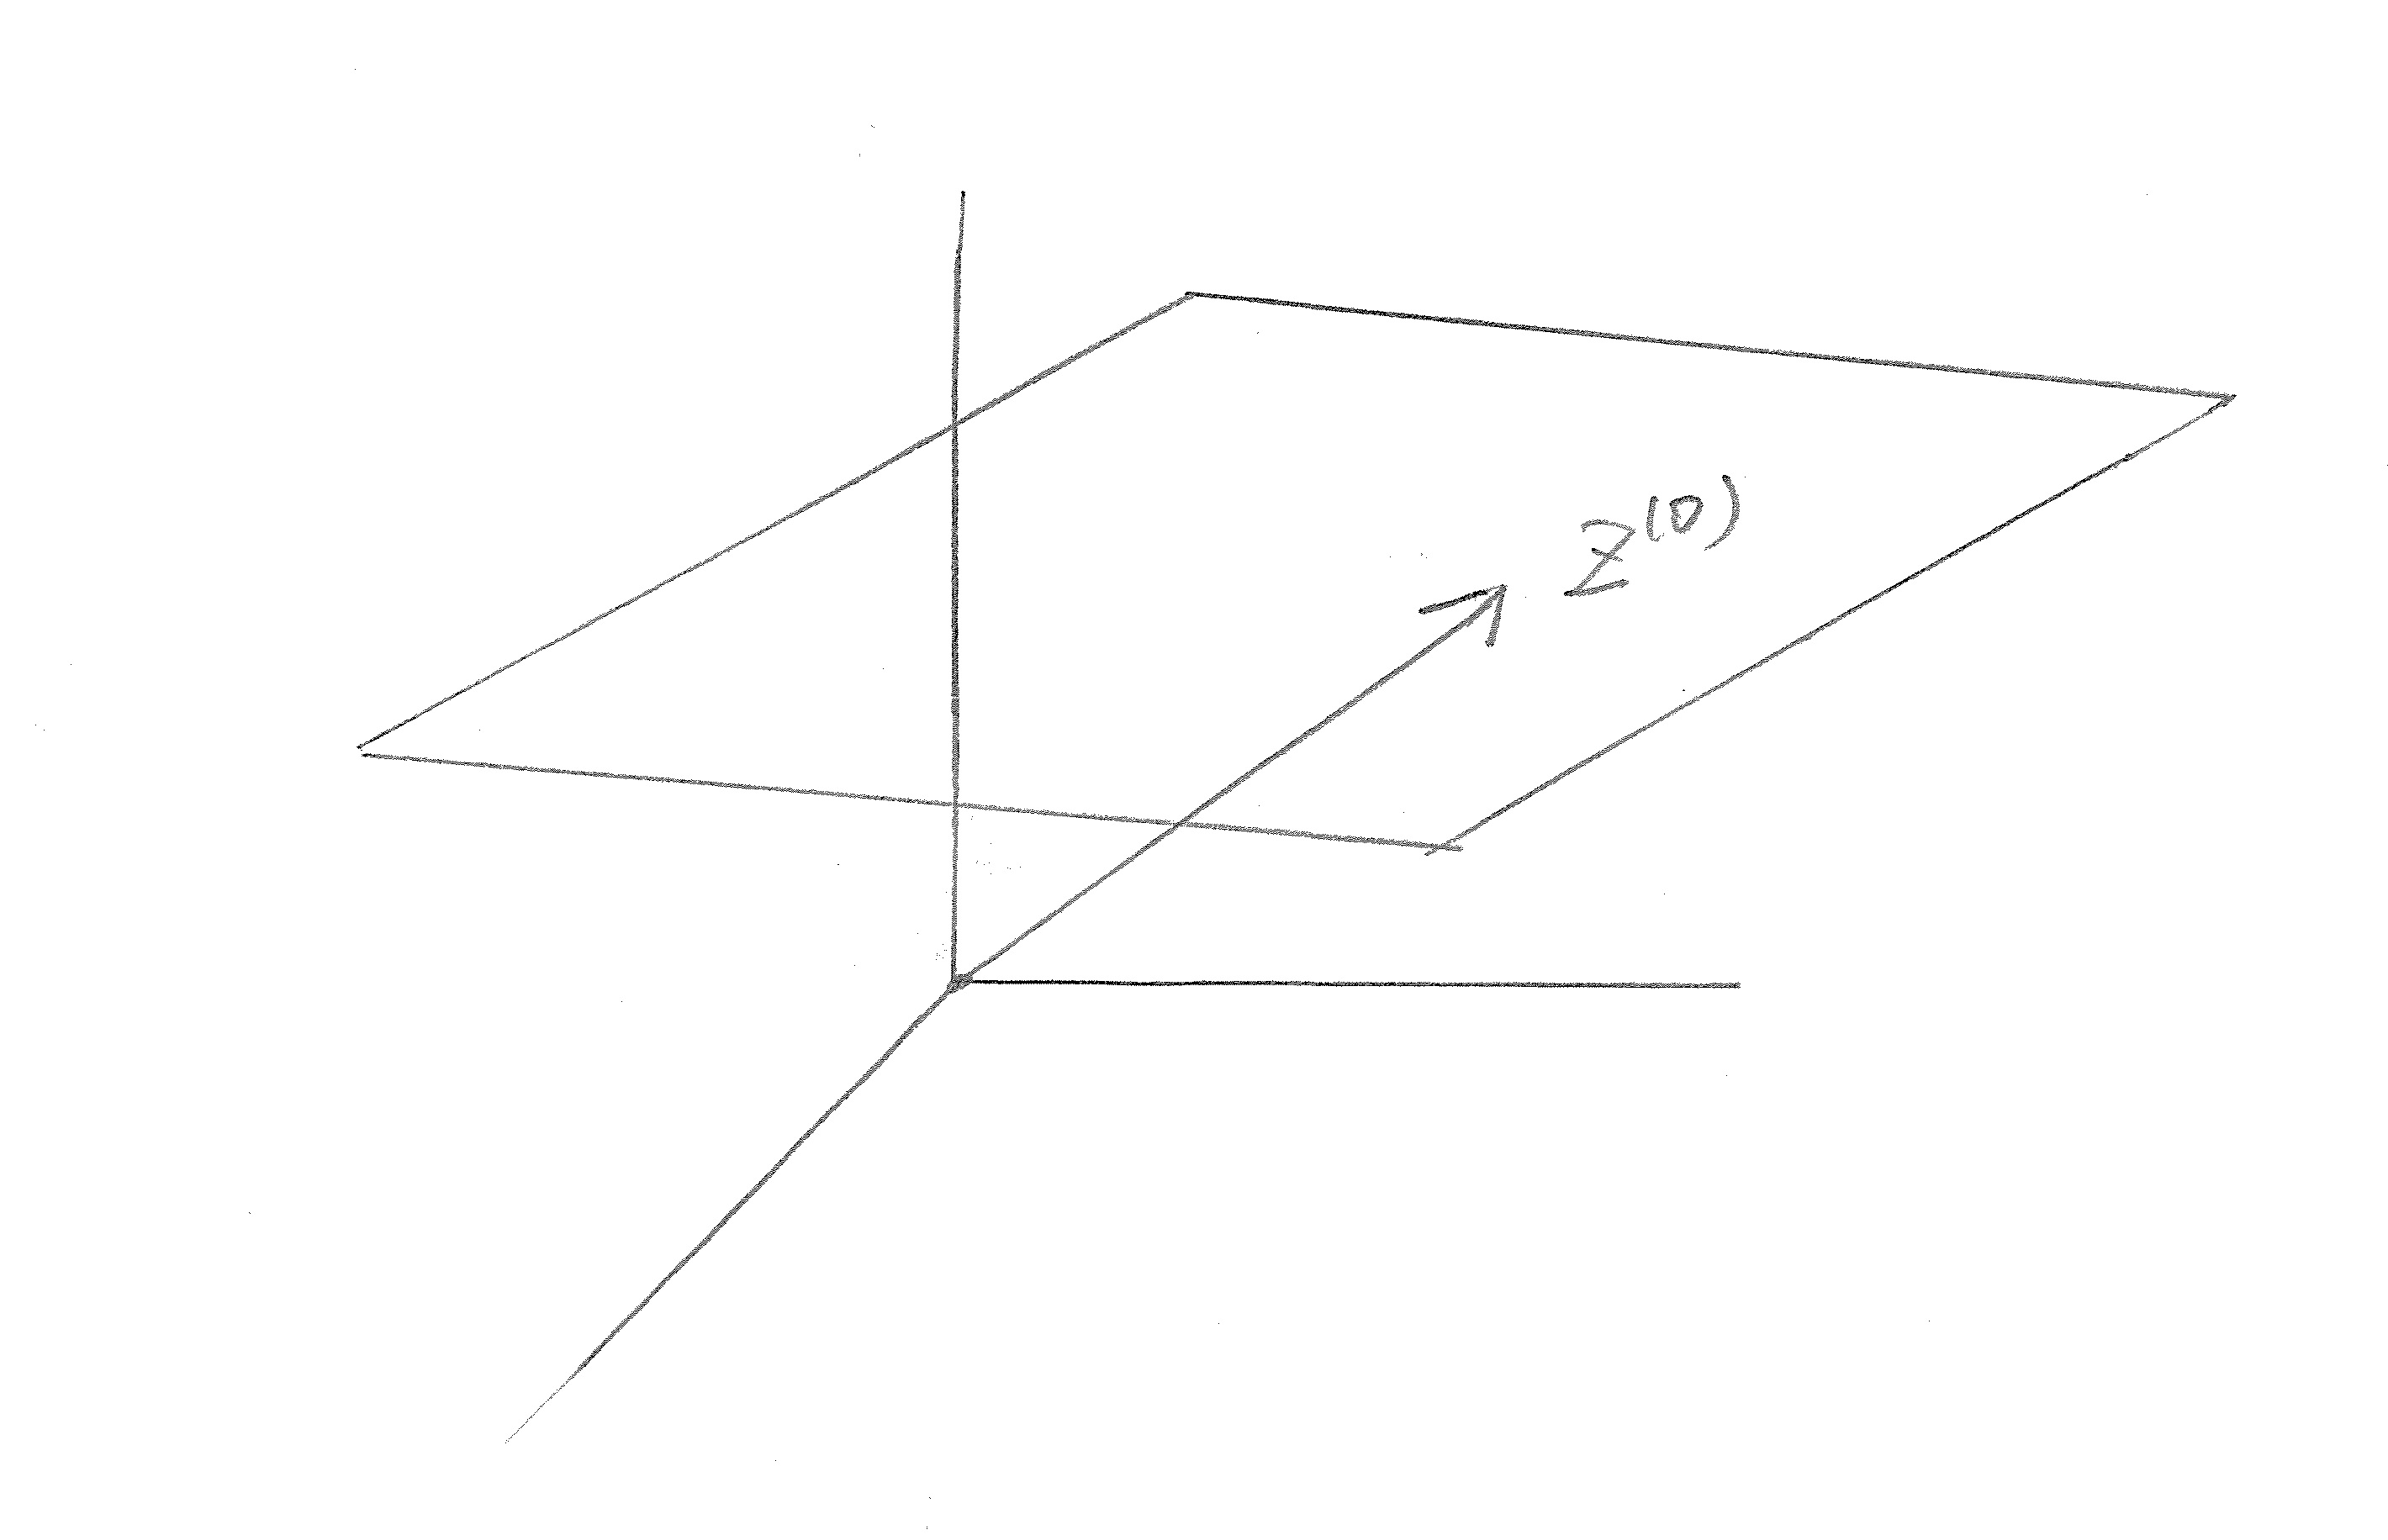
\includegraphics[width=2.1in,height=2.1in]{figures/ch02/p35.jpg}
	%\caption{This is an inserted JPG graphic} 
	%\label{fig:graph} 
\end{figure}

A hyperplane is a special type of affine set. The dimension of the hyperplane is $n-1$ given that the subspace $S$ has a dimension of $n$. For example,

(1) A (2-D) plane is a hyperplane in $\mathbb{R}^3$. 

(2) A line is a hyperplane in $\mathbb{R}^3$. 

(3) A line is not hyperplane in $\reals_{3}$.


\vspace{0.3cm}
Exercise: Prove equivalence of above 2 definition

Let's Start with $\mathcal{H} = \{z \in \mathbb{R}^2 | a^{T} z = b \}$, and let $z^{0} \in \mathcal{H}$(any element at $\mathcal{H}$ will do).

Then, since $a^{T} z^{0} = b$ and for any $z \in \mathcal{H}$, we have

$$a^{T} z - b = 0\Leftrightarrow a^{T} - a^{T}z^{(0)} = 0\Leftrightarrow a^{T} (z - z^{(0)}) = 0$$

Thus,
$$\mathcal{H} = \{z | a^{T} (z - z^{(0)}) = 0 \}     \qquad (*)$$

Now, since $(\text{span} \{ a \}) = \{ x | x= \lambda  a, \lambda \in \mathcal{R} \}$ is a subspace of dim $1$, the set $(\text{span} \{ a \})^{\perp} $ is a subspace of dim $n-1$. 

Let $\mathcal{S}$ be this subspace.

Observe that by (*), vectors in $\mathcal{H}$ when translate by $-z^{(0)}$ on $\mathcal{S}$. 

Therefore $\mathcal{H}$ is $\mathcal{S}$ translated by $+z^{(0)}$ yields $z^{(0)}$. 

Now, let's start with $\mathcal{H} = \{ z \in \mathbb{R}^n | z = u + z^{(0)}, u \in \mathcal{S}, z \in \mathcal{H} \}$. 

Let $\{ u^{(1)}, \dots, u^{(n-1)} \}$ be a basis for $u$, and we choose $a \perp u^{(i)}$, $i \in [n-1]$ and let $b = a^{T} z^{0}$. Then for any $z \in \mathcal{H}$, we have $a^{T} z = 0 + a^{T} z^{(0)} = b$. 


\vspace{0.3cm}
Example: 2-D case.
Let normal direction be $a = (1, \frac{1}{2})$, offset $b = 2$.
\begin{align*}
\mathcal{H} &= \{z \in \mathbb{R}^2 | a^{T} z = b \} \\
&= \{z \in \mathbb{R}^2 | z_1 + \frac{1}{2} z_2 - 2 = 0 \}
\end{align*}


\begin{figure}
	\centering
	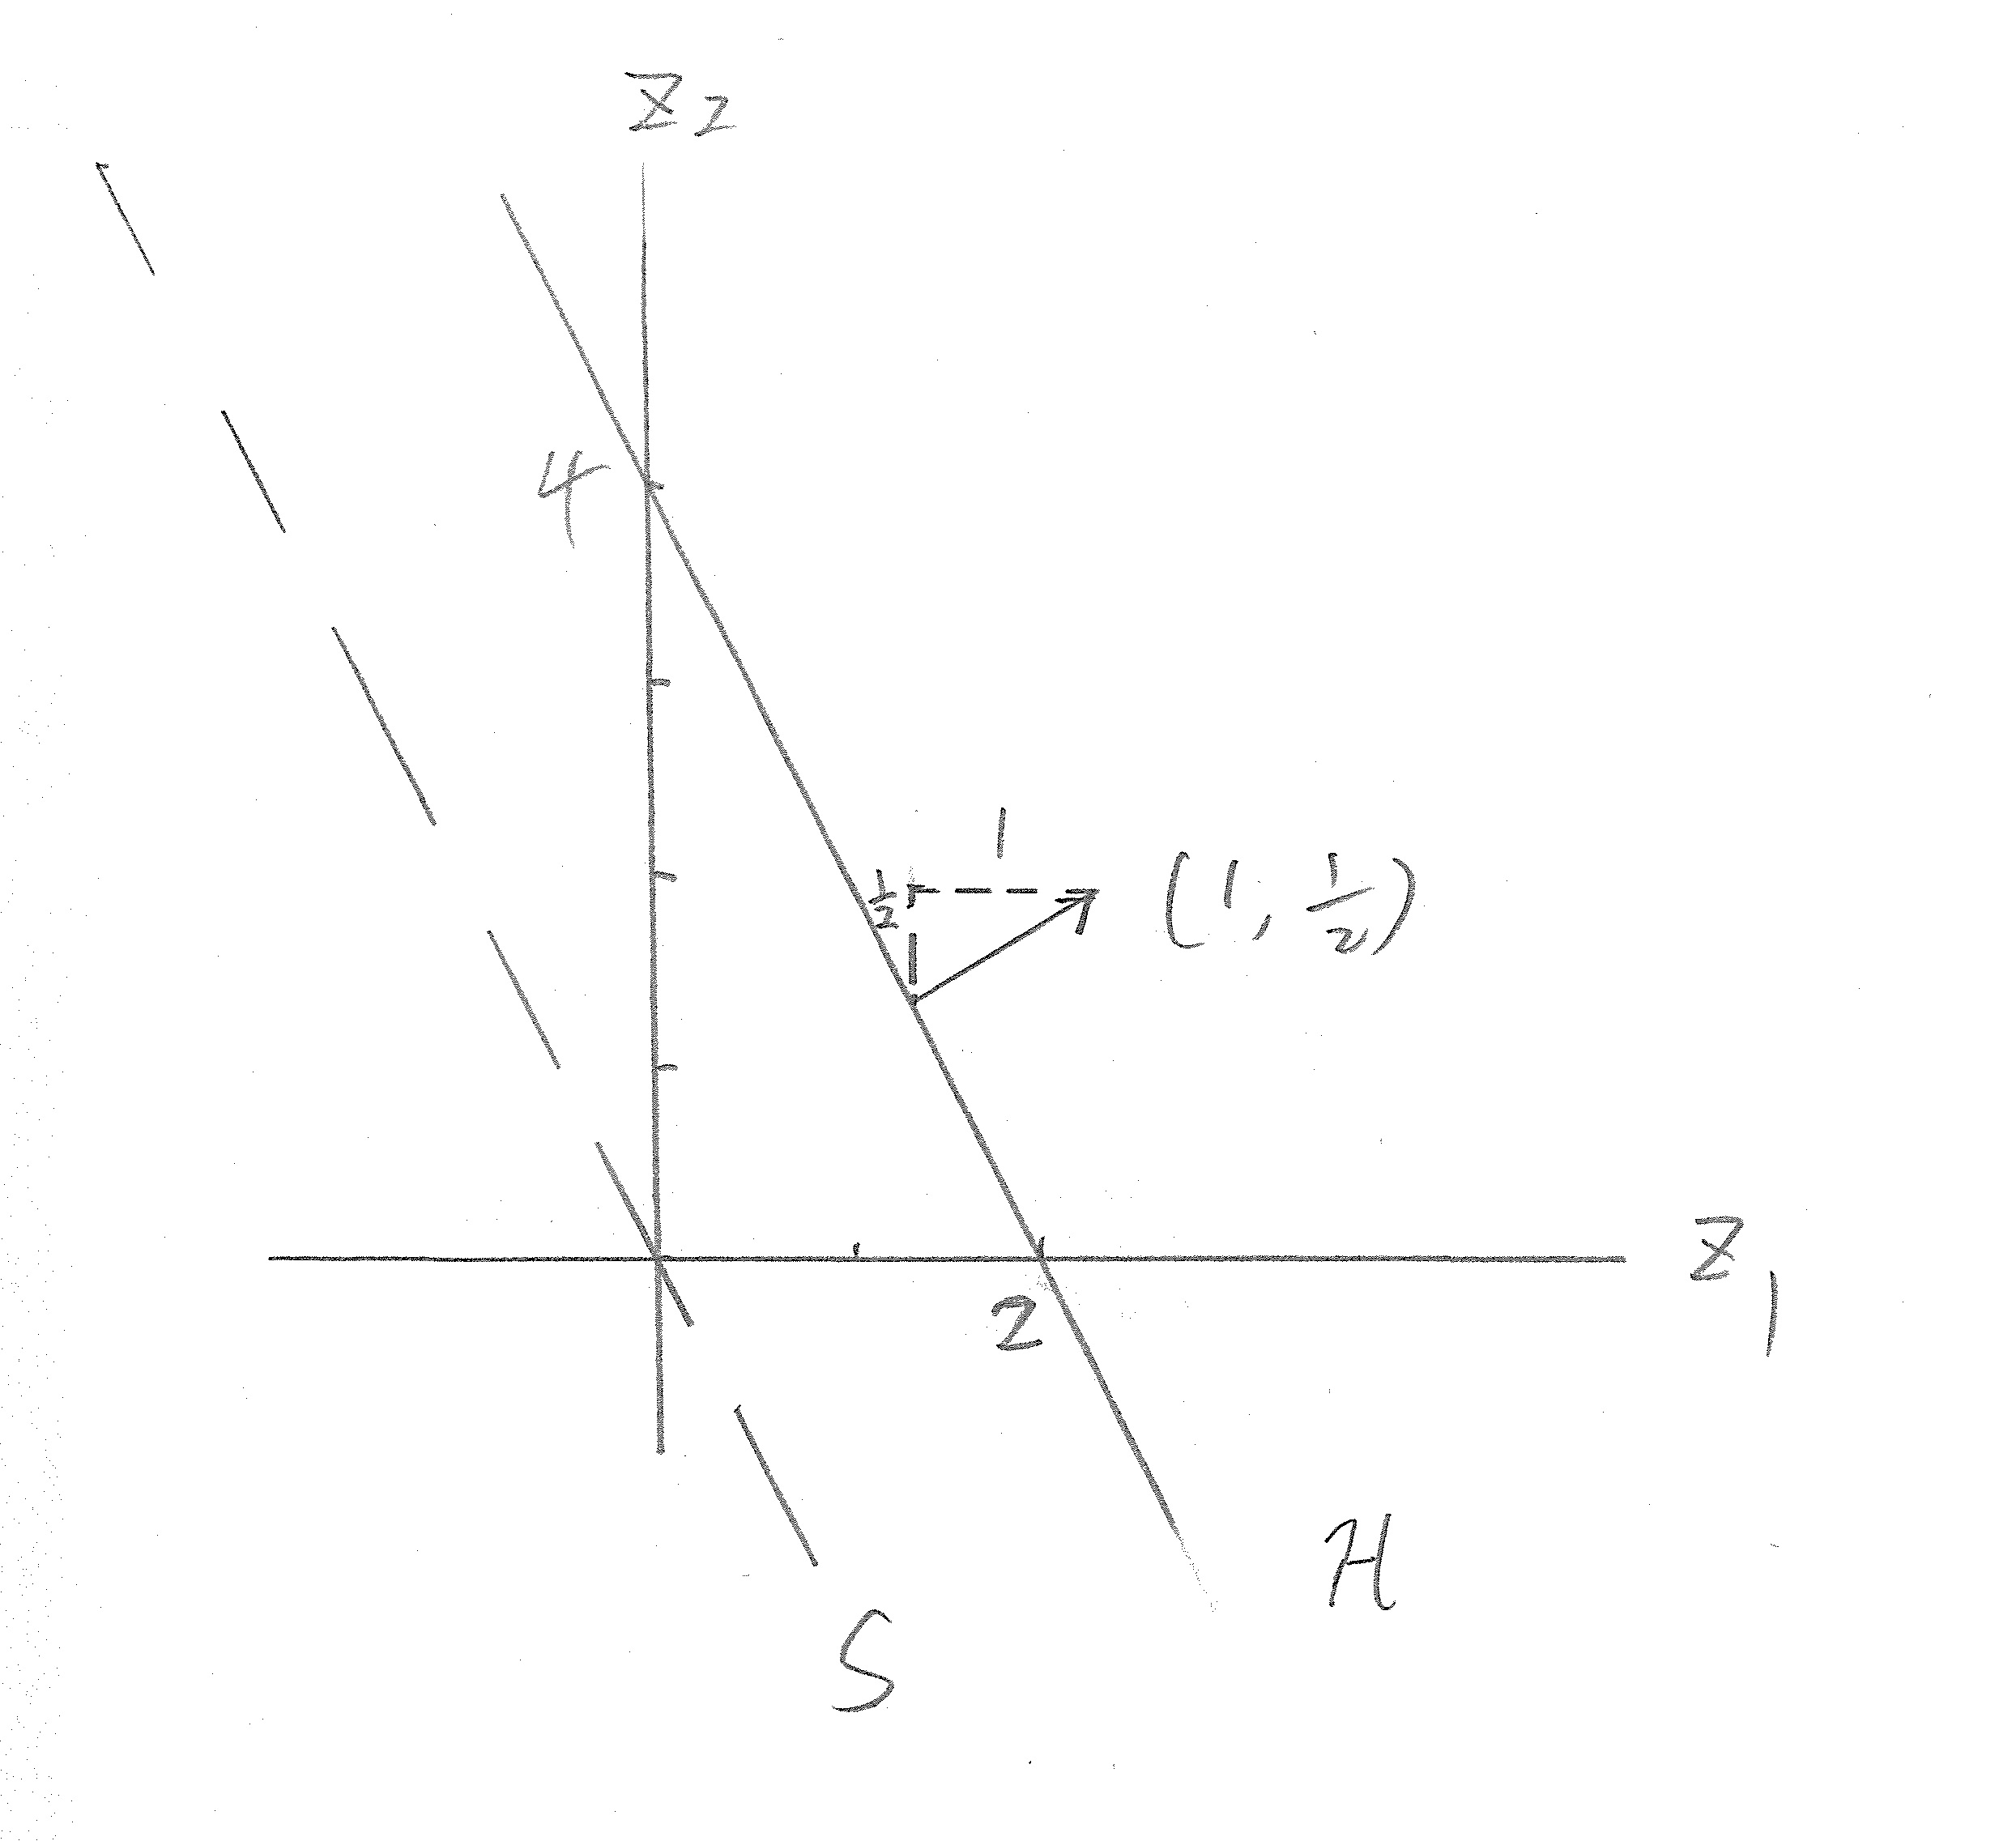
\includegraphics[width=2.1in,height=2.1in]{figures/ch02/p37.jpg}
	%\caption{This is an inserted JPG graphic} 
	%\label{fig:graph} 
\end{figure}


$\mathcal{H} = \{ z \in \mathbb{R}^n \vert z = u + z^{(0)}, u \in \mathcal{S}, z^{(0)} = \begin{bmatrix} 2\\ 0\\ \end{bmatrix} \}$

when 
\begin{align*}
\mathcal{S} &= \{z \in \mathbb{R}^2 | a^{T} z = 0 \} \\
&= \{z \in \mathbb{R}^2 | z_1 + \frac{1}{2} z_2 = 0 \}
\end{align*}

Note that recall any value at $z^{(0)} \in \mathcal{H}$ works so alternatively, e.g.,
$$\mathcal{H} = \{ z \in \mathbb{R}^n | z = u + z^{(0)}, u \in S, z^{(0)} = \begin{bmatrix} 0\\ 4\\ \end{bmatrix} \}$$
or 
$$\mathcal{H} = \{ z \in \mathbb{R}^n | z = u + z^{(0)}, u \in S, z^{(0)} = \begin{bmatrix} 1\\ 2\\ \end{bmatrix} \}\quad \text{, etc.} $$

\vspace{0.3cm}
Now let's back to the first example, projection onto hyperplane.
$$\mathcal{H}=\{z\in\reals^{n}\vert a^{\trans} z=b\}=\{z\in\reals^{n}|z=x_{s}+z^{(0)},x_{s}\in S, z^{(0)}\in \mathcal{H}\}$$

\begin{figure}
	\centering
	\resizebox{7.5cm}{3cm}{%% page 39

\def\RightAngle[size=#1](#2,#3,#4){%
 \draw ($(#3)!#1!(#2)$) -- 
       ($($(#3)!#1!(#2)$)!#1!90:(#2)$) --
       ($(#3)!#1!(#4)$);
 \path (#3) --
 ($($(#3)!#1!(#2)$)!#1!90:(#2)$);
}

\begin{tikzpicture}
\draw[thick,-stealth] (-3, 0) -- (3, 0);
\draw[thick,-stealth] (0, -2) -- (0, 4);

\coordinate (A) at (-3, -1.5);
\coordinate (B) at (3, 1.5);
\coordinate (C) at (-0.8, 1.1);
\draw (A) -- (B) node[right]{$\mathcal{S}$};

\coordinate (A1) at (-4, -0.5);
\coordinate (B1) at (3, 3);
\coordinate (C1) at (0.8, 3.4);
\draw (A1) -- (B1) node[right]{$\mathcal{A}$};

\coordinate (D1) at ($(A1)!(C1)!(B1)$);
\draw[dashed] (C1)node[above]{$p$} -- ($(A1)!(C1)!(B1)$)node[below right]{$p^{*}$};
%% right angle
\RightAngle[size=10pt](C1,D1,A1);

\end{tikzpicture}}
	\caption{}
	\label{}
\end{figure}

Recall that $\text{dim}(S)=n-1$, so $\text{dim}(S^{\perp})=1$, and we want to find the point $p^{*}=\arg \min_{p\in \mathcal{H}} \Vert p^{*}-p\Vert$.

Observe that $(p-p^{*}) \perp S$ (by optimal condition), So $(p-p^{*}) \in S^{\perp}=\{\lambda a|\lambda \in \reals \}$, and $\exists \lambda^{*}$ such that $p-p^{*}=\lambda^{*}a$.

Now, we want to solve for $\lambda^{*}$ but notice that there are 2 unknowns $(\lambda^{*},p^{*})$, and hence we get rid of $p^{*}$ dependency by using definition of $\mathcal{H}$.
\begin{align*}
&\qquad p-p^{*}=\lambda^{*}a\\
&\Leftrightarrow a^{\trans} (p-p^{*})=a^{\trans} (\lambda^{*}a)\\
&\Leftrightarrow a^{\trans} p-a^{\trans} p^{*}=\lambda^{*}a^{\trans} a\\
&\Leftrightarrow a^{\trans} p-b=\lambda^{*}a^{\trans} a\\
&\Leftrightarrow \lambda^{*}=\frac{a^{\trans} p-b}{a^{\trans} a}\\
&\Leftrightarrow \lambda^{*}=\frac{a^{\trans} p-b}{\Vert a\Vert^{2}}\\
\end{align*}

Thus, $p-p^{*}=\lambda^{*} a=(\frac{a^{\trans} p-b}{\Vert a\Vert^{2}})a$, or $p^{*}=p-(\frac{a^{\trans} p-b}{\Vert a\Vert^{2}})a$.

and 
$$\Vert p-p^{*}\Vert=\Vert \lambda^{*}a\Vert= \vert \lambda^{*}\vert \Vert a\Vert=\frac{\vert a^{\trans} p-b\vert}{\Vert a\Vert}$$.

Recall terminology $\Vert p-p^{*}\Vert=\min_{y\in \mathcal{H}} \Vert y-p\Vert$, we have
$$p^{*}=\arg\min_{y\in \mathcal{H}} \Vert y-p\Vert$$


\vspace{0.5cm}
\noindent\textbf{Projection w.r.t other norms}

Recall that inner product spaces have a notion of angle, have term "orthogonality principle", and the $L_{2}$ norm is one such example. In contrast, some norms such as $L_{1}$ and$ L_{\infty}$ norms don't come with a sense of angle. However the problem still make senses if $p\neq 2$, e.g., $p=1$, $p=\infty$, but we cannot apply $\perp$ principle since there is no sense of angle.

\vspace{0.3cm}
In following we will

(1). Discuss projection in normed vector spaces, particularly $L_{1}$ and $L_{\infty}$.

(2). Illustrate how the solution differs as you change the norm (change $p$).

(3). Give you a sense for character of difference such for $p=1$ and $p=\infty$.

(4). Get a sense of why might pick $p\neq 2$.

\newpage
Recall norm balls we draw before. Let's project $0\in\reals^{2}$ onto a line (affine set/hyperplane).

\begin{marginfigure}
	\centering
	\resizebox{7.5cm}{3cm}{%% page 42
%% fig 1
\begin{tikzpicture}
\draw[thick,-stealth] (-2, 0) -- (2, 0);
\draw[thick,-stealth] (0, -2) -- (0, 2);

\draw (0,0) circle [radius=1];
\node [below right] at (1, 0) { };

\end{tikzpicture}
}
	\caption{}
	\label{}
\end{marginfigure}

\begin{marginfigure}
	\centering
	\resizebox{7.5cm}{3cm}{%% page 42
%% fig 2
\begin{tikzpicture}
\draw[thick,-stealth] (-2, 0) -- (2, 0);
\draw[thick,-stealth] (0, -2) -- (0, 2);

\draw (-1, 0) -- (0, 1) -- (1, 0) -- (0, -1) -- (-1, 0);
\node [below right] at (1, 0) { };
\end{tikzpicture}
}
	\caption{}
	\label{}
\end{marginfigure}

\begin{marginfigure}
	\centering
	\resizebox{7.5cm}{3cm}{%% page 42
%% fig 3
\begin{tikzpicture}
\draw[thick,-stealth] (-2, 0) -- (2, 0);
\draw[thick,-stealth] (0, -2) -- (0, 2);

\draw (-1, -1) rectangle (1, 1);
\node [below right] at (1, 0) { };

\end{tikzpicture}

}
	\caption{}
	\label{}
\end{marginfigure}


\begin{figure}
	\centering
	\resizebox{7.5cm}{3cm}{%% page 42
%% fig 4
\begin{tikzpicture}
\draw[thick,-stealth] (-3, 0) -- (5, 0);
\draw[thick,-stealth] (0, -2) -- (0, 4);

\coordinate (O) at (0, 0) node[below right]{$O$};
\coordinate (A) at (-2, 2);
\coordinate (B) at (4.5, -1);
\draw (A) -- (B) node[right]{$\mathcal{A}$};
\end{tikzpicture}}
	\caption{}
	\label{}
\end{figure}

$$x^{*}=\arg\min_{x\in \mathcal{A}} \Vert x-0\Vert_{p}=\arg\min_{x\in \mathcal{A}} \Vert x\Vert_{p}$$


\begin{figure}
	\centering
	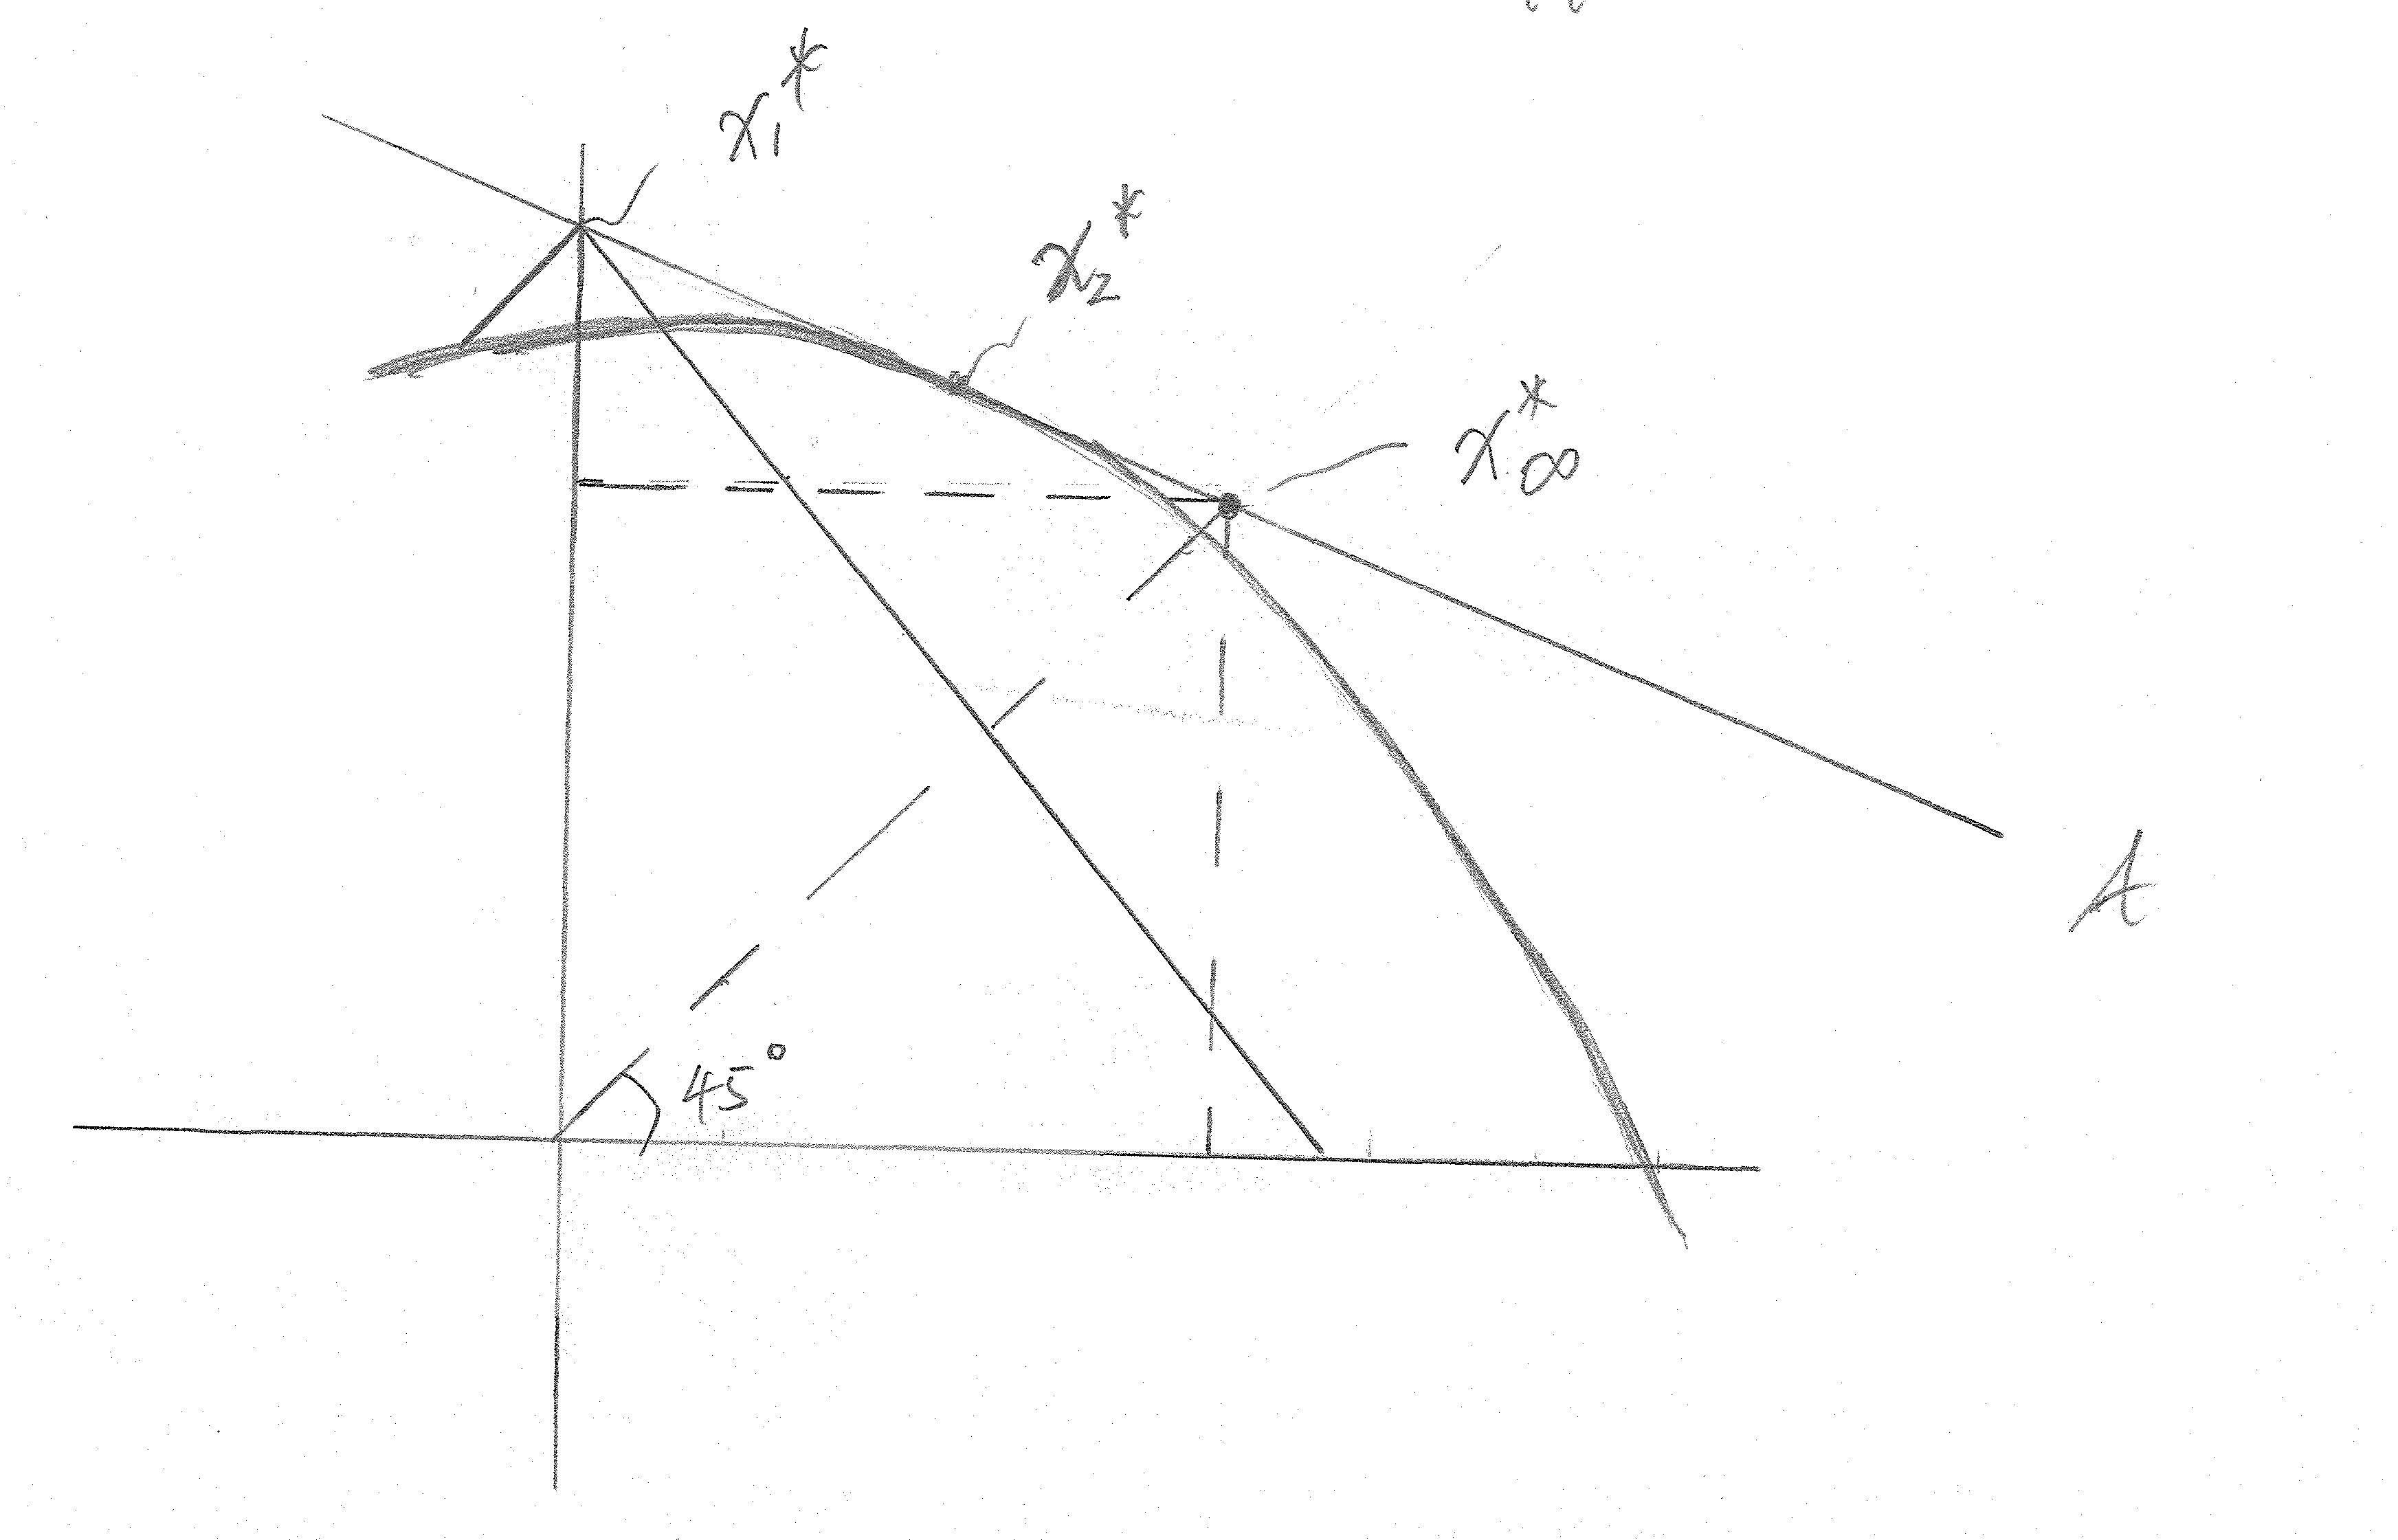
\includegraphics[width=2.1in,height=2.1in]{figures/ch02/p43.jpg}
	%\caption{This is an inserted JPG graphic} 
	%\label{fig:graph} 
\end{figure}


Observe that:

$x_{2}^{*}$: Familiar with solution via inner product and $\perp$ theorem, and has a closed form solution.

$x_{1}^{*}$: Solution is "sparse", generally will be the case for affine constraints since vertices of norm-ball are axis-aligned.

$x_{\infty}^{*}$: At optimum, $x_{\infty, 1}^{*}=x_{\infty, 2}^{*}$, equal-magnitude coordinate.


\vspace{0.5cm}
\noindent\textbf{Functions}

Some terminologies will be used in this material:

"Function":  $F:\reals^{n}\mapsto \reals$

"Map":  $F:\reals^{n}\mapsto \reals^{m}$


However, not all input values may be allowed, input may be a subset of $\Omega$ (cf, $\reals^{n}$), this is the "domain" of $F$.% that is
%$$\text{dom} F= \{x\in\reals^{n}|\vert F(x)\vert\leq\infty\}$$

\vspace{0.5cm}
Aside: Terminology when discussion a pair of vector space $(\cal{V},\cal{U})$ over a field $\mathbb{F}$

$F:\cal{U}\mapsto \cal{V}$, a "map", generally $\text{dim}(\cal{U})\neq \text{dim}(\cal{V})$.

$F:\cal{U}\mapsto \cal{U}$ , an "operator", input and output vectors spaces have the same dimension.

$F:\cal{U}\mapsto \mathbb{F}$ , a "functional", map vector space into a scalar.

In this course, $\cal{U}$=$\reals^{n}$, $\cal{V}$=$\reals^{m}$, $\mathbb{F}$=$\reals$ (or, occasionally $\complex$).


\vspace{0.3cm}
\textbf{Sets related to functions}

Various sets defined by a function tell us a lot(or sometimes everything) about a function $F:\reals^{n}\mapsto\reals$

(1) The "graph" (a.k.a, "plot") of $F$ is the set
$$F=\{(x,F(x))\in\reals^{n+1}:x\in\reals^{n}\}$$

(2) The "epigraph" of $F$ is the set 
$$F=\{(x,t)\in\reals^{n+1}:x\in\reals^{n}, t\geq F(x) \}$$

\begin{marginfigure}
	\centering
	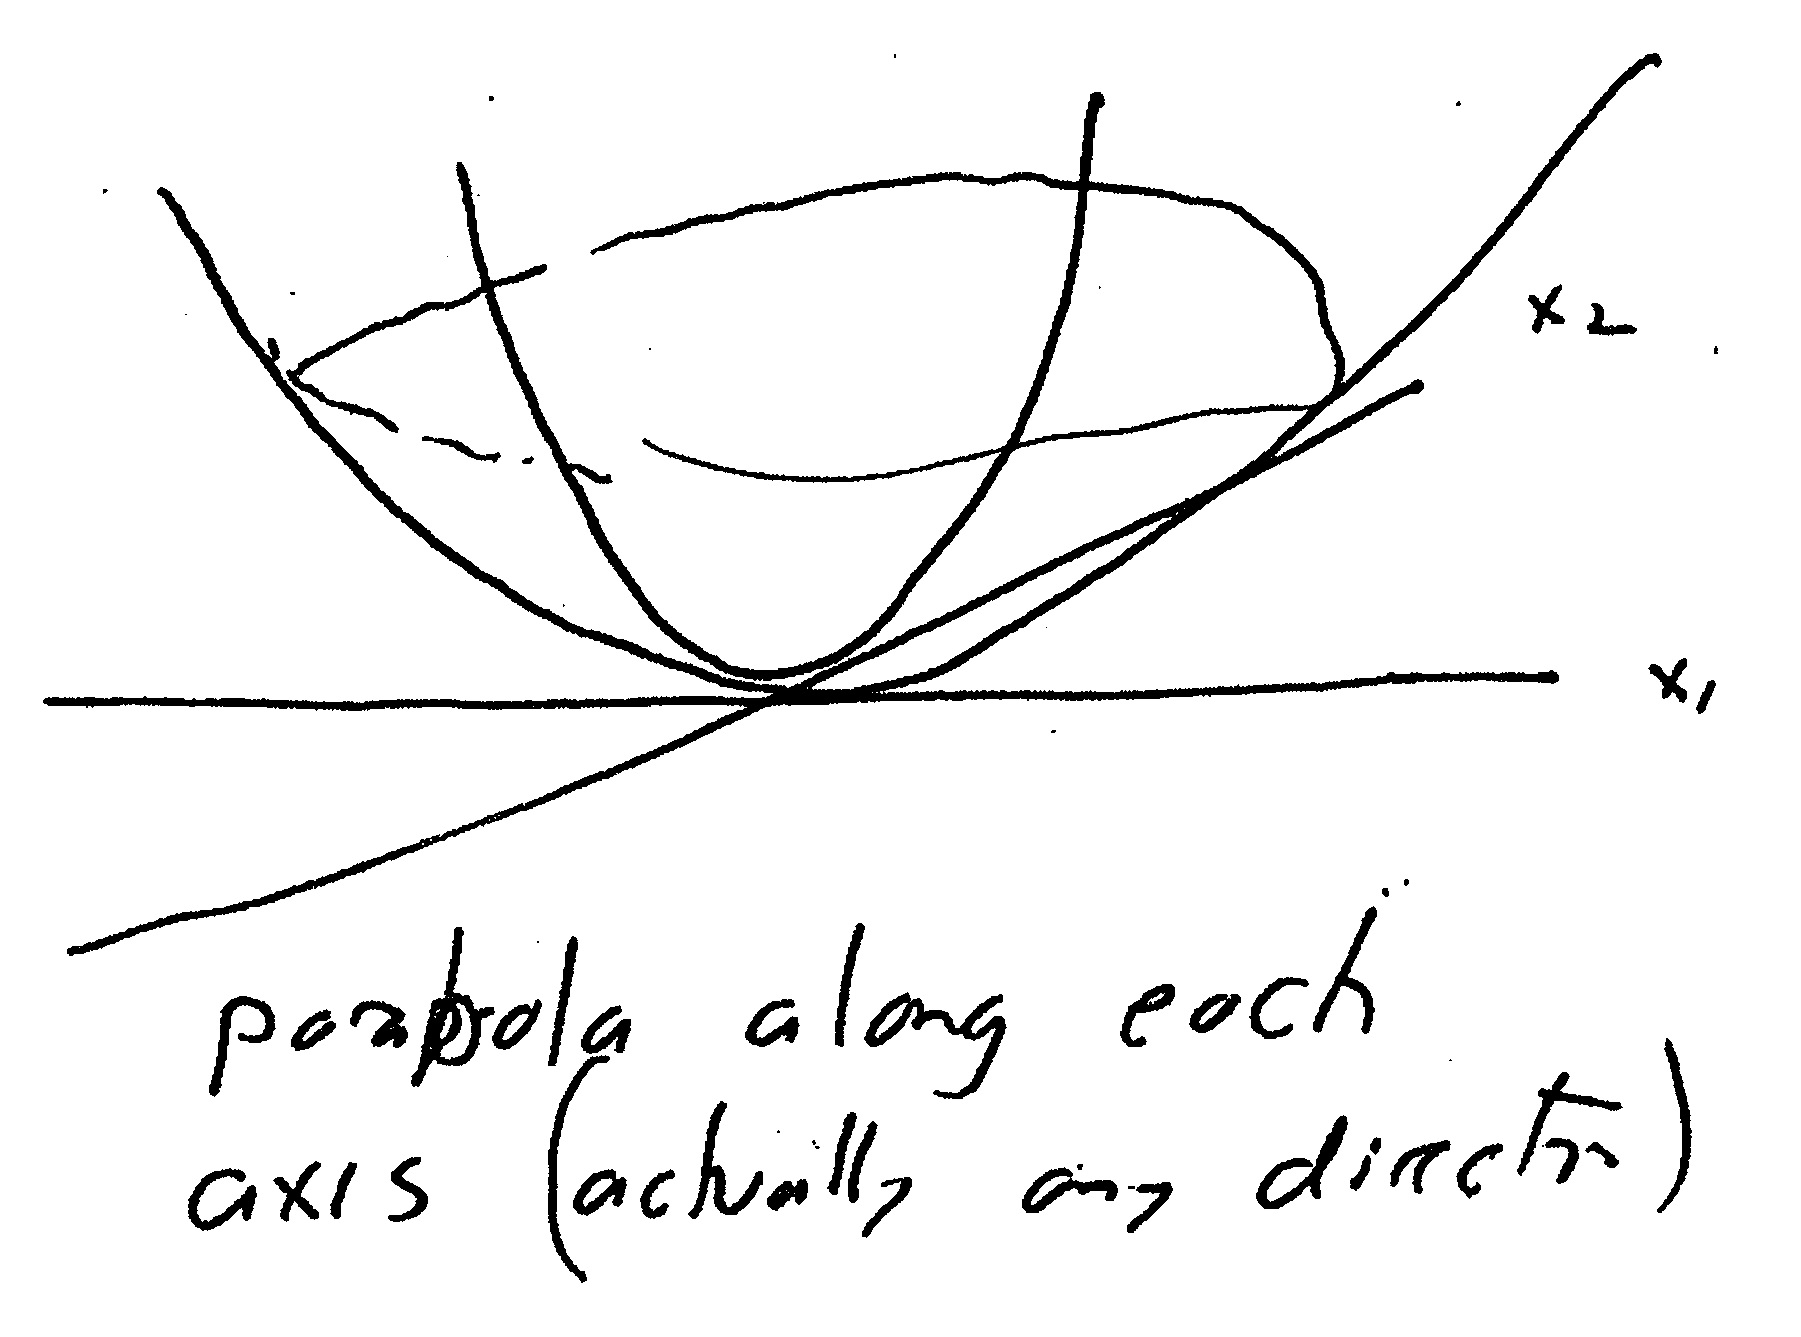
\includegraphics[width=2.1in,height=2.1in]{figures/ch02/p48-1.jpg}
	\caption{Graph 1} 
	%\label{fig:graph} 
\end{marginfigure}

\begin{marginfigure}
	\centering
	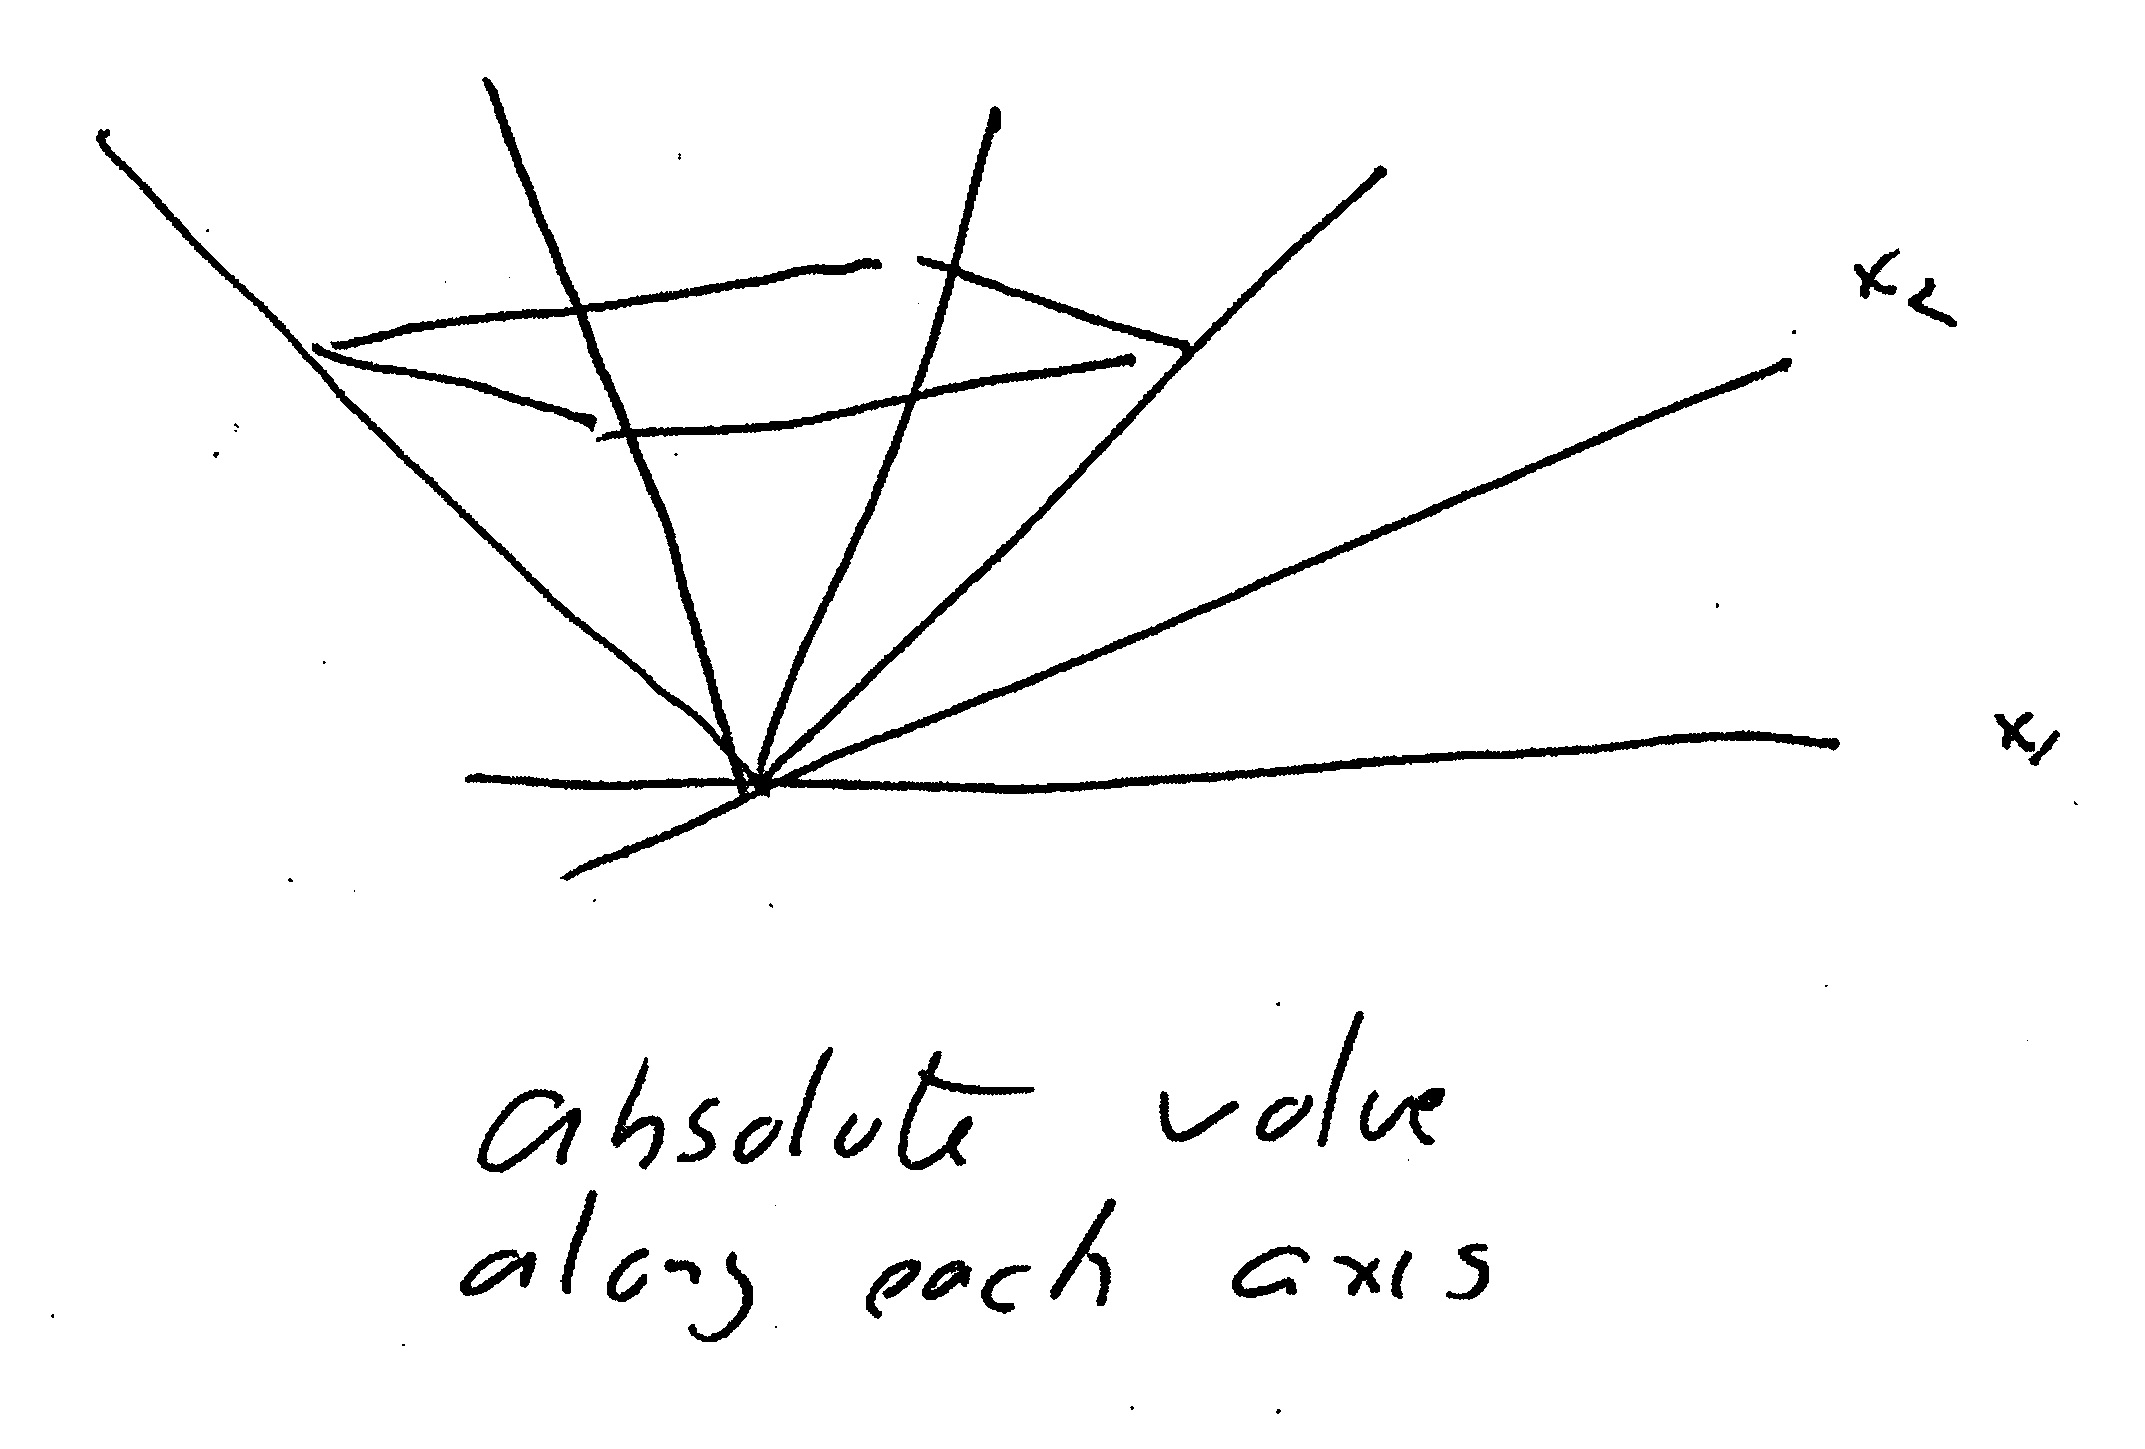
\includegraphics[width=2.1in,height=2.1in]{figures/ch02/p48-2.jpg}
	\caption{Graph 2} 
	%\label{fig:graph} 
\end{marginfigure}

\begin{marginfigure}
	\centering
	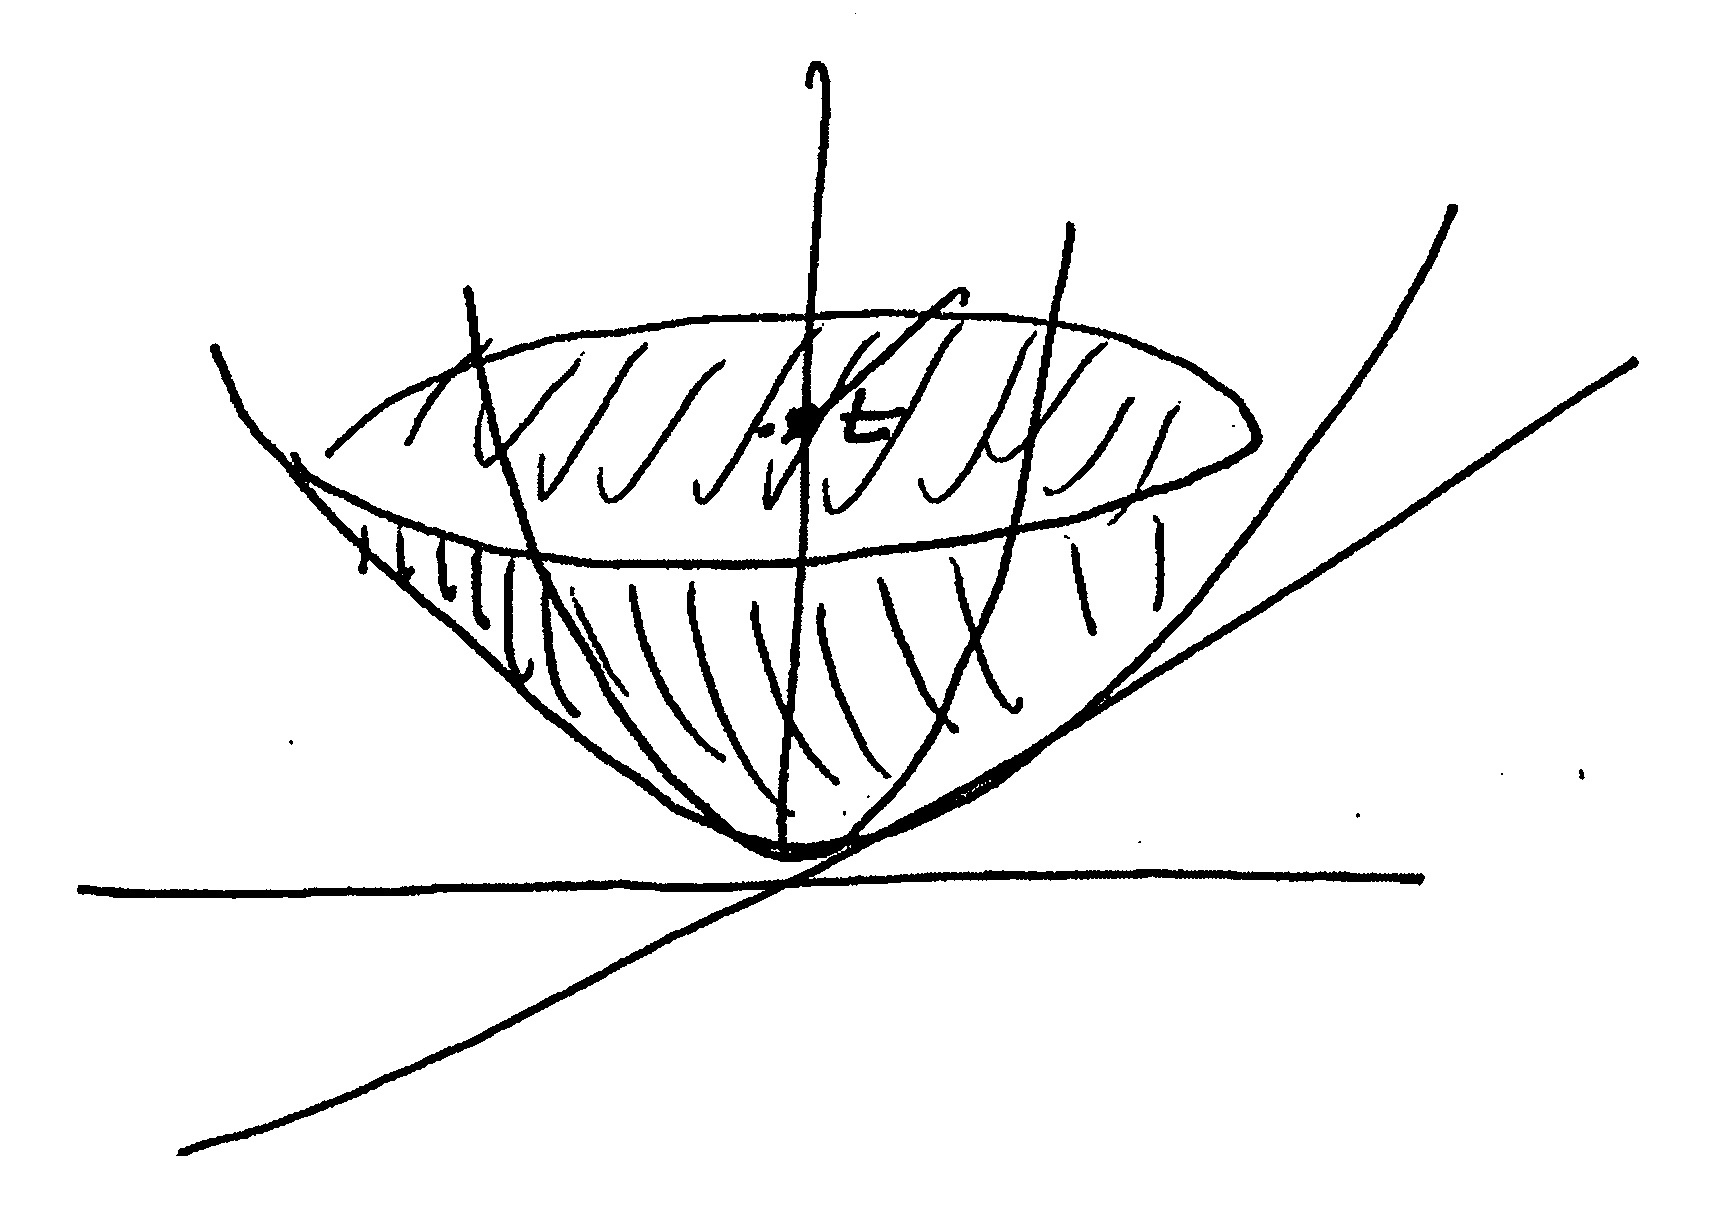
\includegraphics[width=2.1in,height=2.1in]{figures/ch02/p48-3.jpg}
	\caption{Epigraph 1} 
	%\label{fig:graph} 
\end{marginfigure}

\begin{marginfigure}
	\centering
	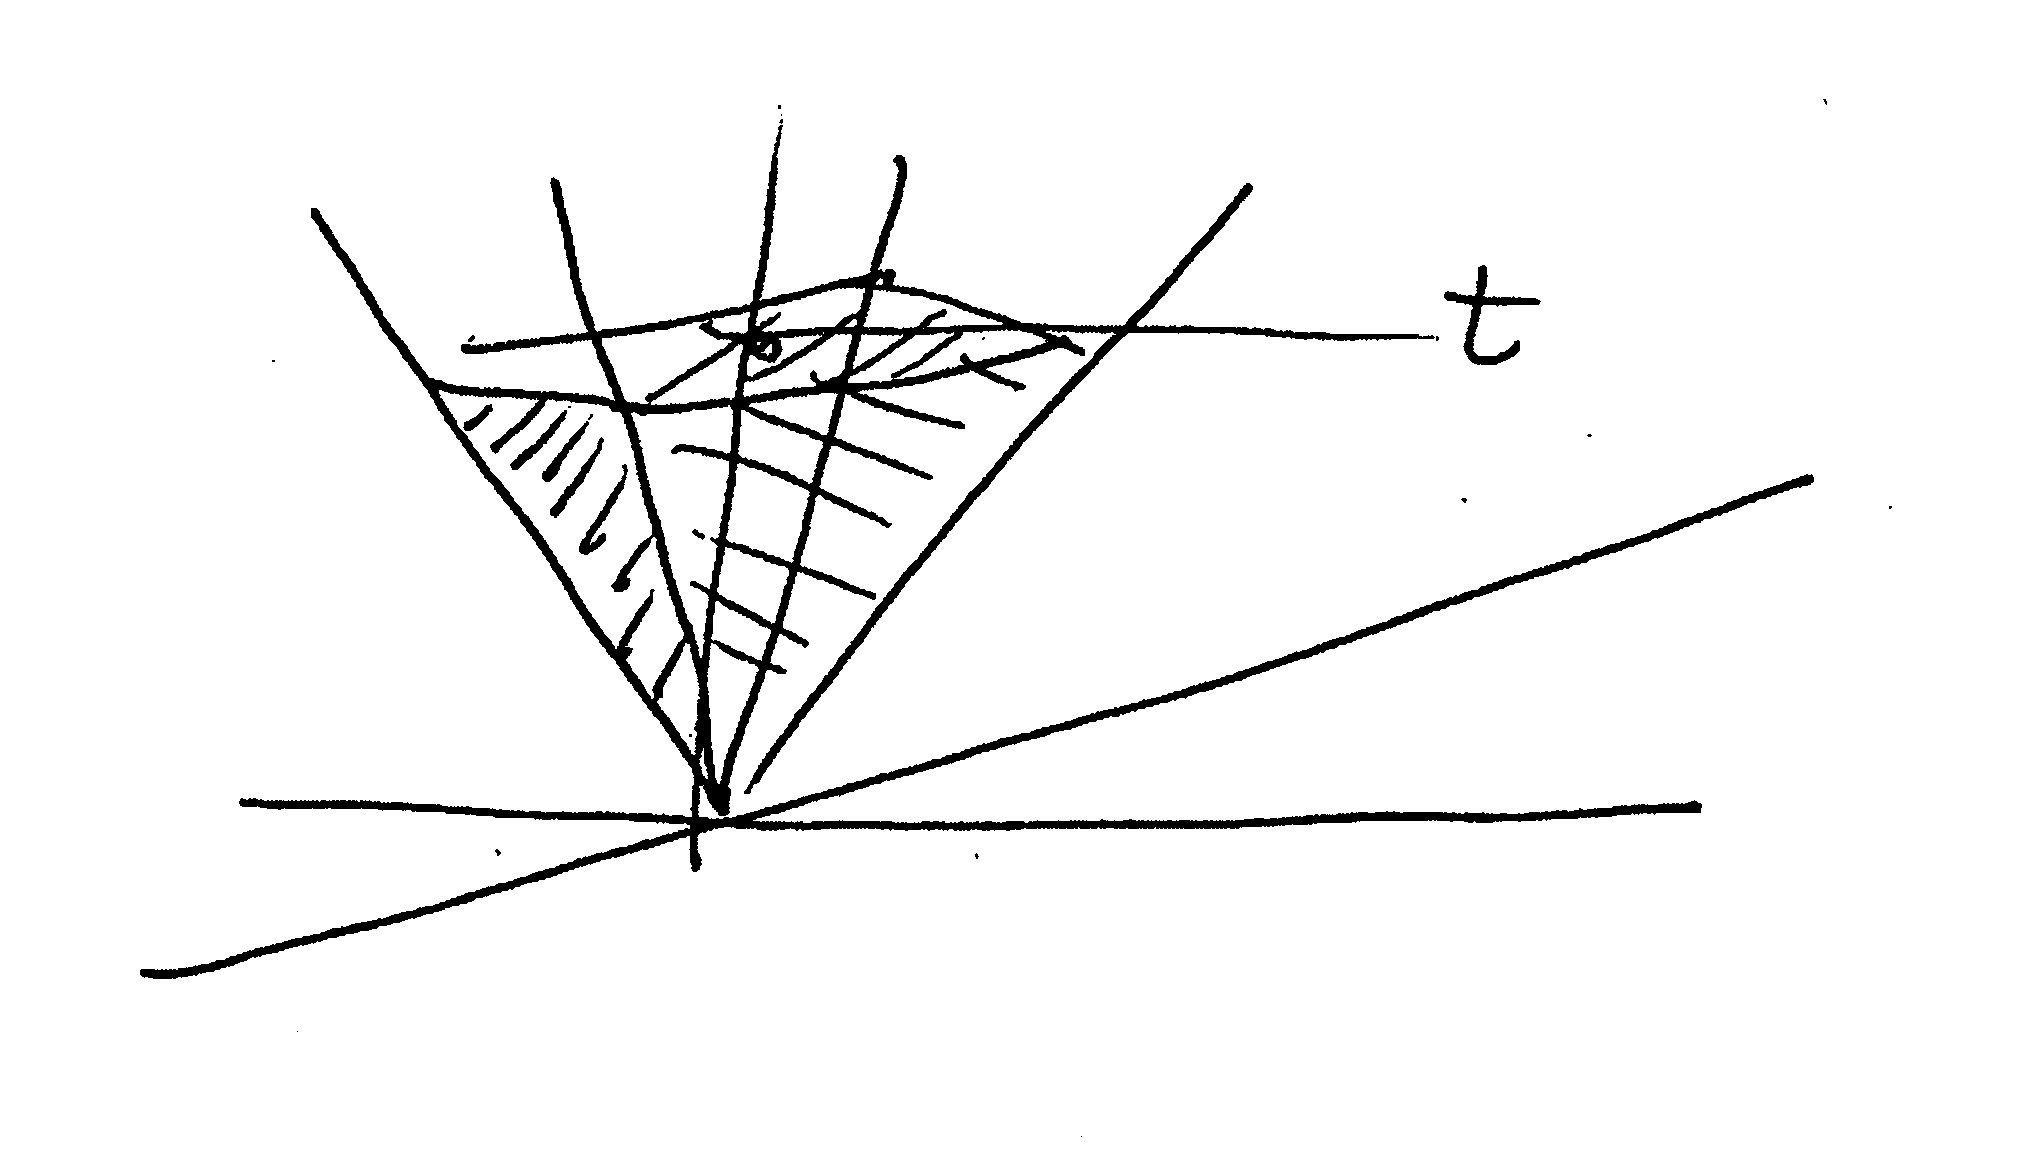
\includegraphics[width=2.1in,height=2.1in]{figures/ch02/p48-4.jpg}
	\caption{Epigraph 2} 
	%\label{fig:graph} 
\end{marginfigure}


Graph
\begin{figure}
	\centering
	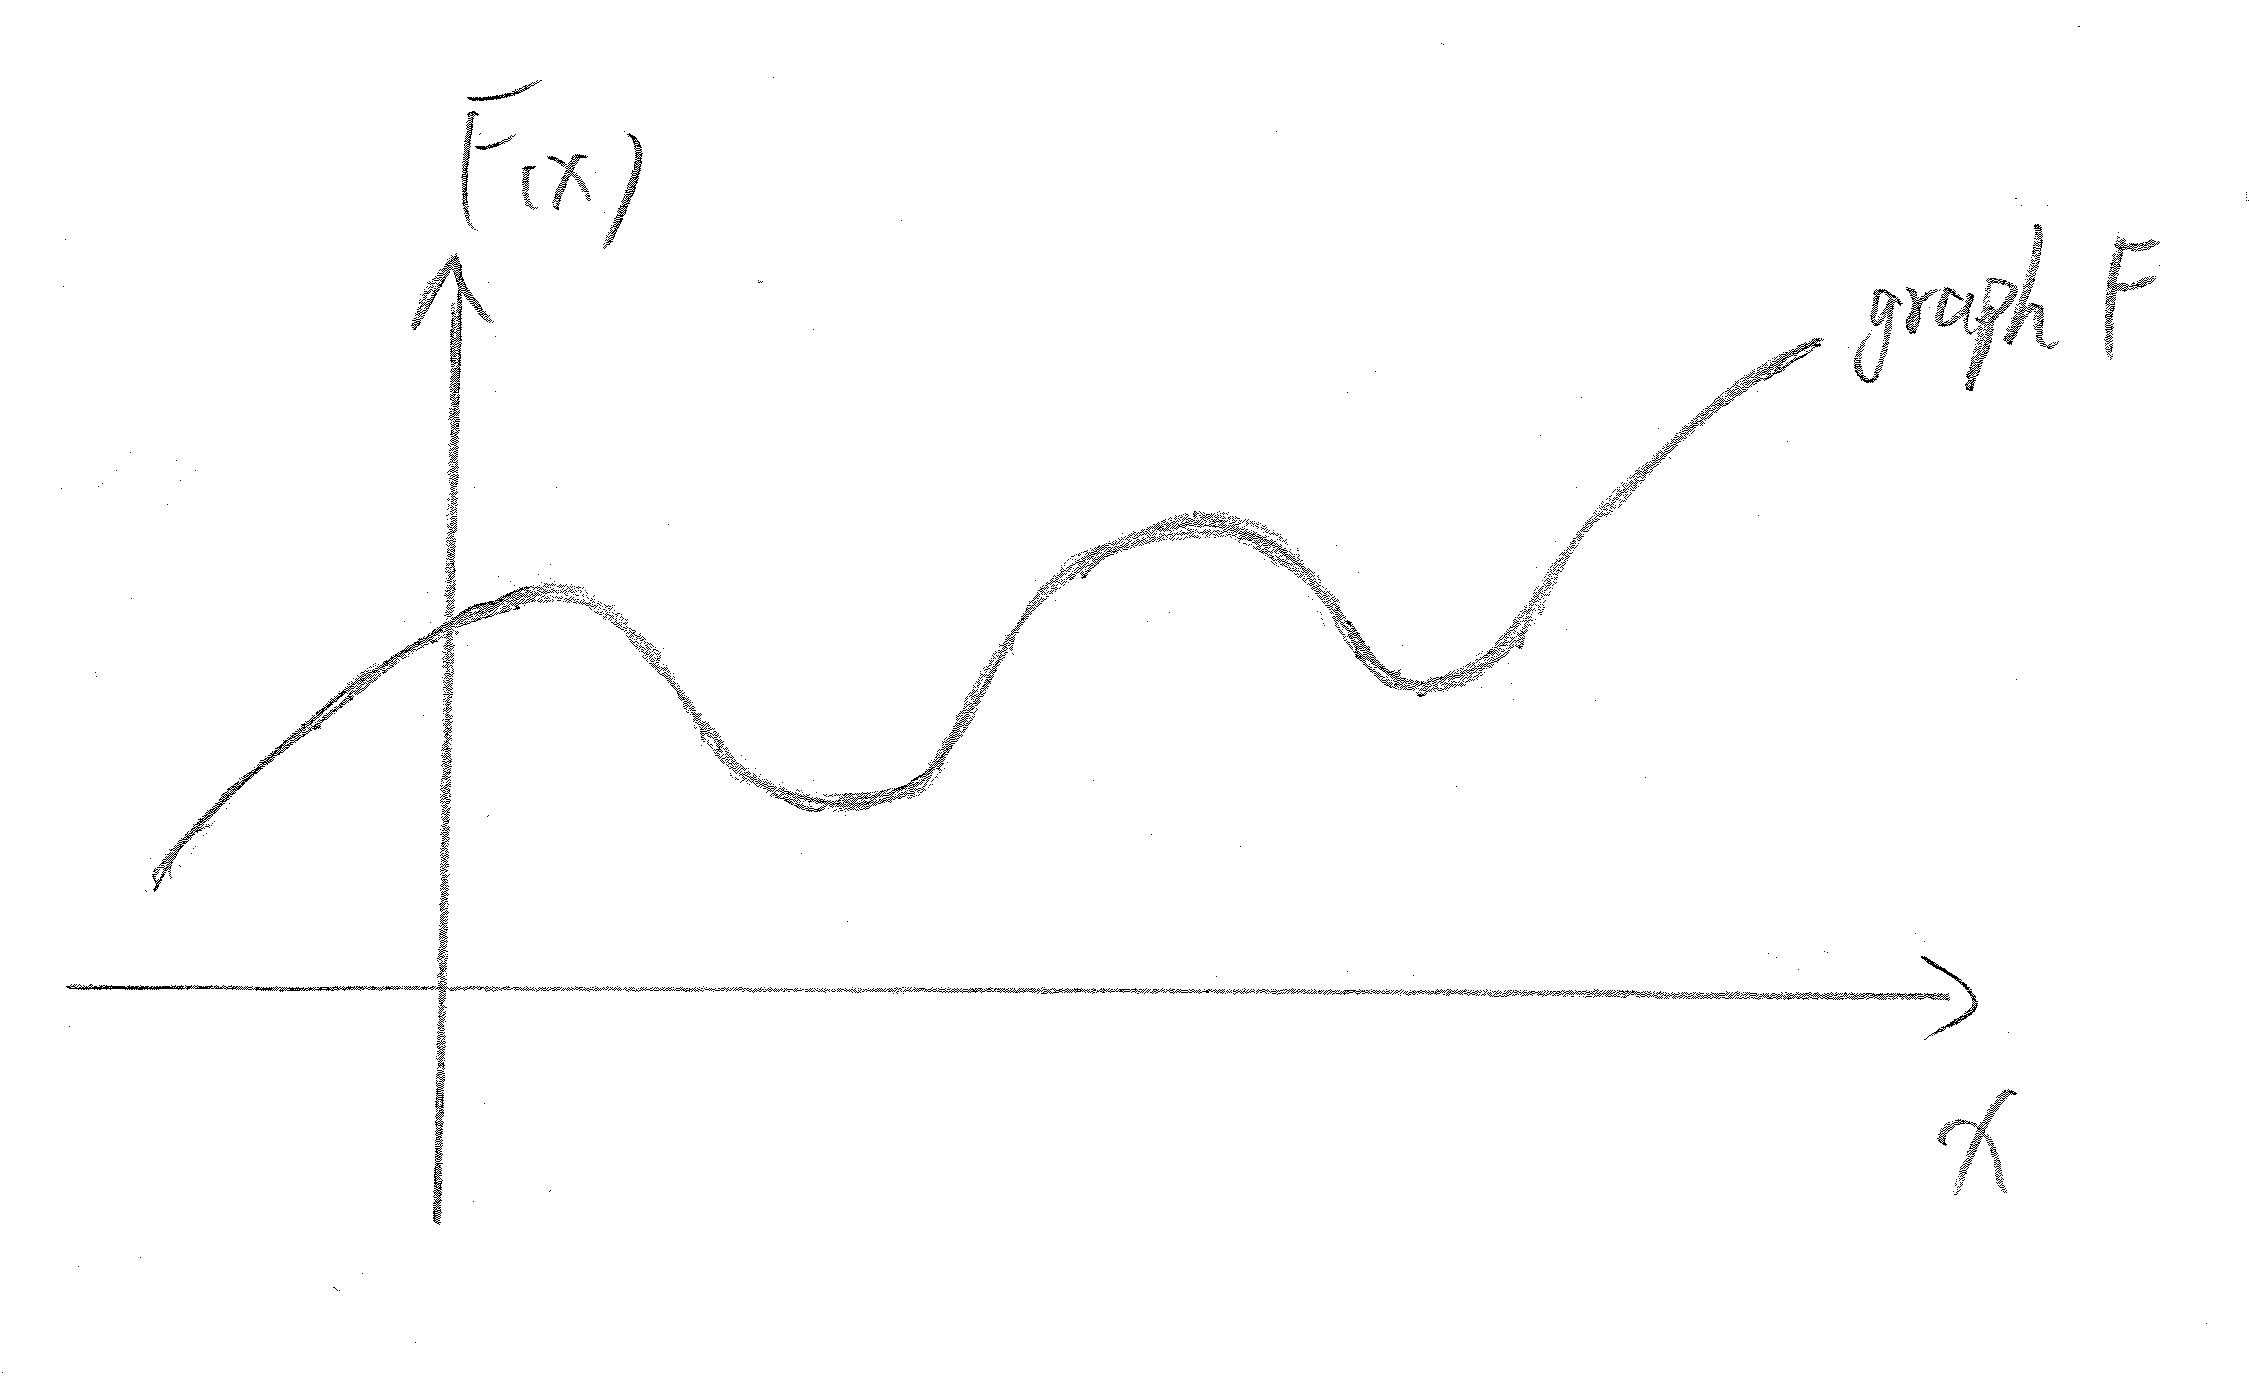
\includegraphics[width=2.1in,height=2.1in]{figures/ch02/p47-1.jpg}
	%\caption{This is an inserted JPG graphic} 
	\label{fig:graph} 
\end{figure}

Epigraph
\begin{figure}
	\centering
	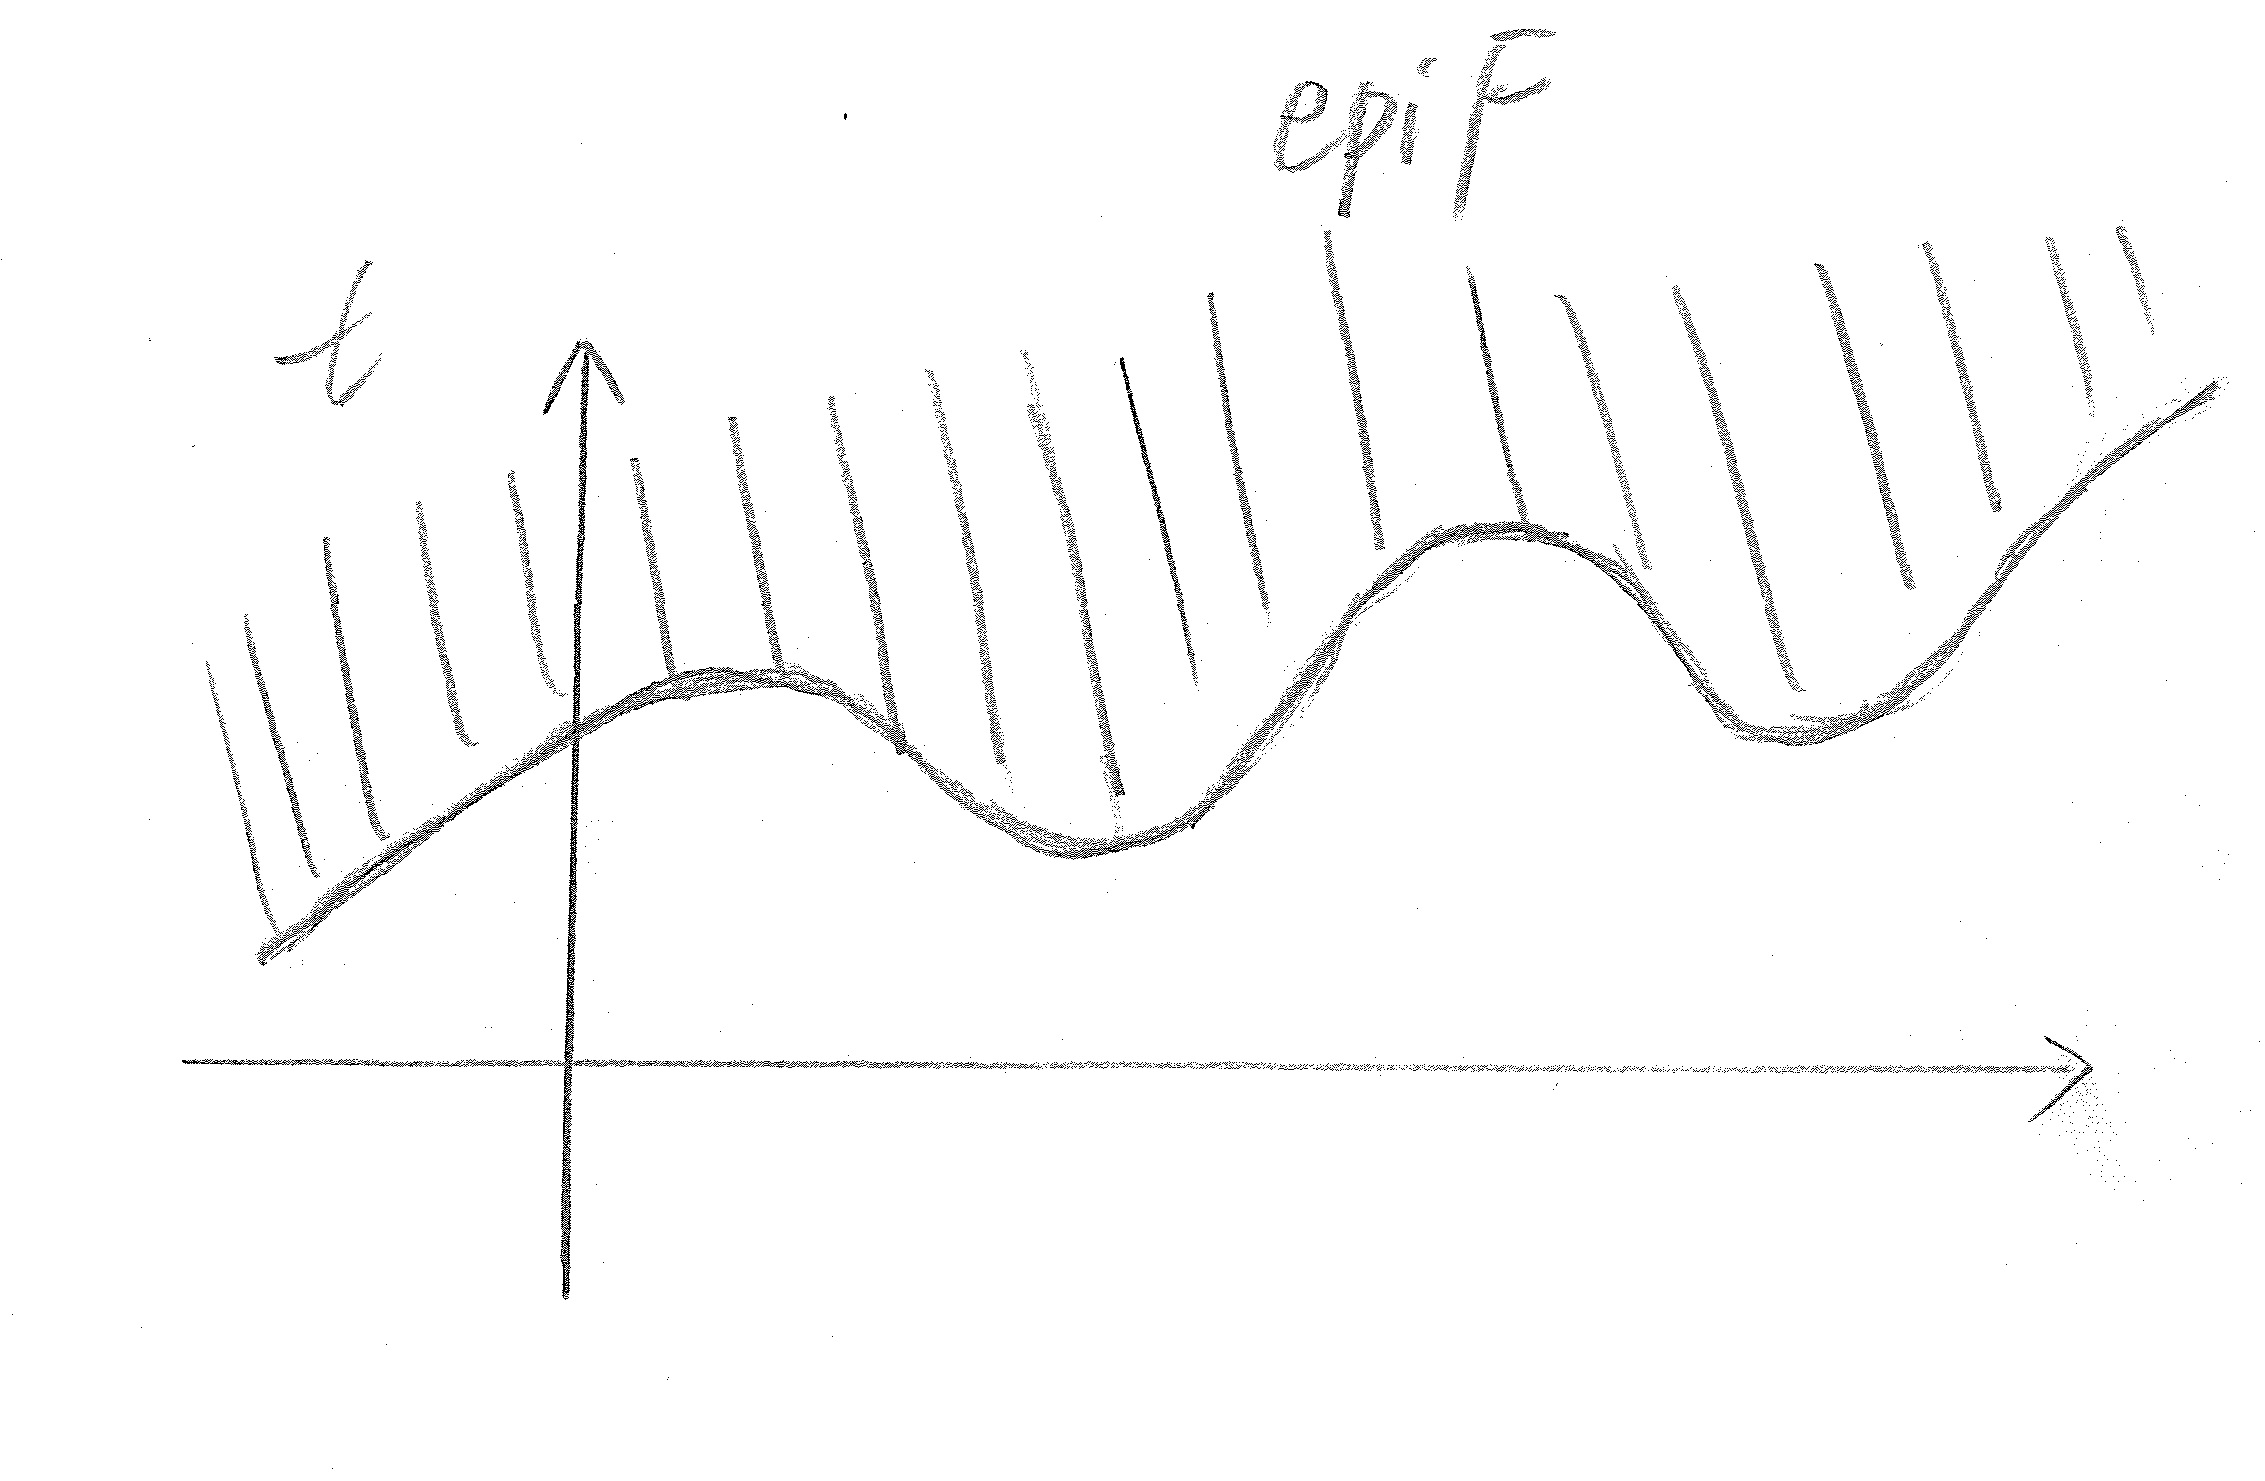
\includegraphics[width=2.1in,height=2.1in]{figures/ch02/p47-2.jpg}
	%\caption{This is an inserted JPG graphic} 
	%\label{fig:graph} 
\end{figure}



It is also useful to consider points at(or below) a height

(3) The "level" set
$$c_{F}(t)=\{x\in\reals^{n}:F(x)=t\}$$

(4) The "sub-level" set
$$L_{F}(t)=\{x\in\reals^{n}:F(x)\leq t\}$$

Note: graph and epigraph are in $\reals^{n+1}$, level and sublevel set are in $\reals^{n}$


\vspace{0.5cm}
Let's sketch these sets for $L_{2}$ and $L_{1}$ norms in $\reals^{2}$ on the r.h.s.

\newpage

\begin{marginfigure}
	\centering
	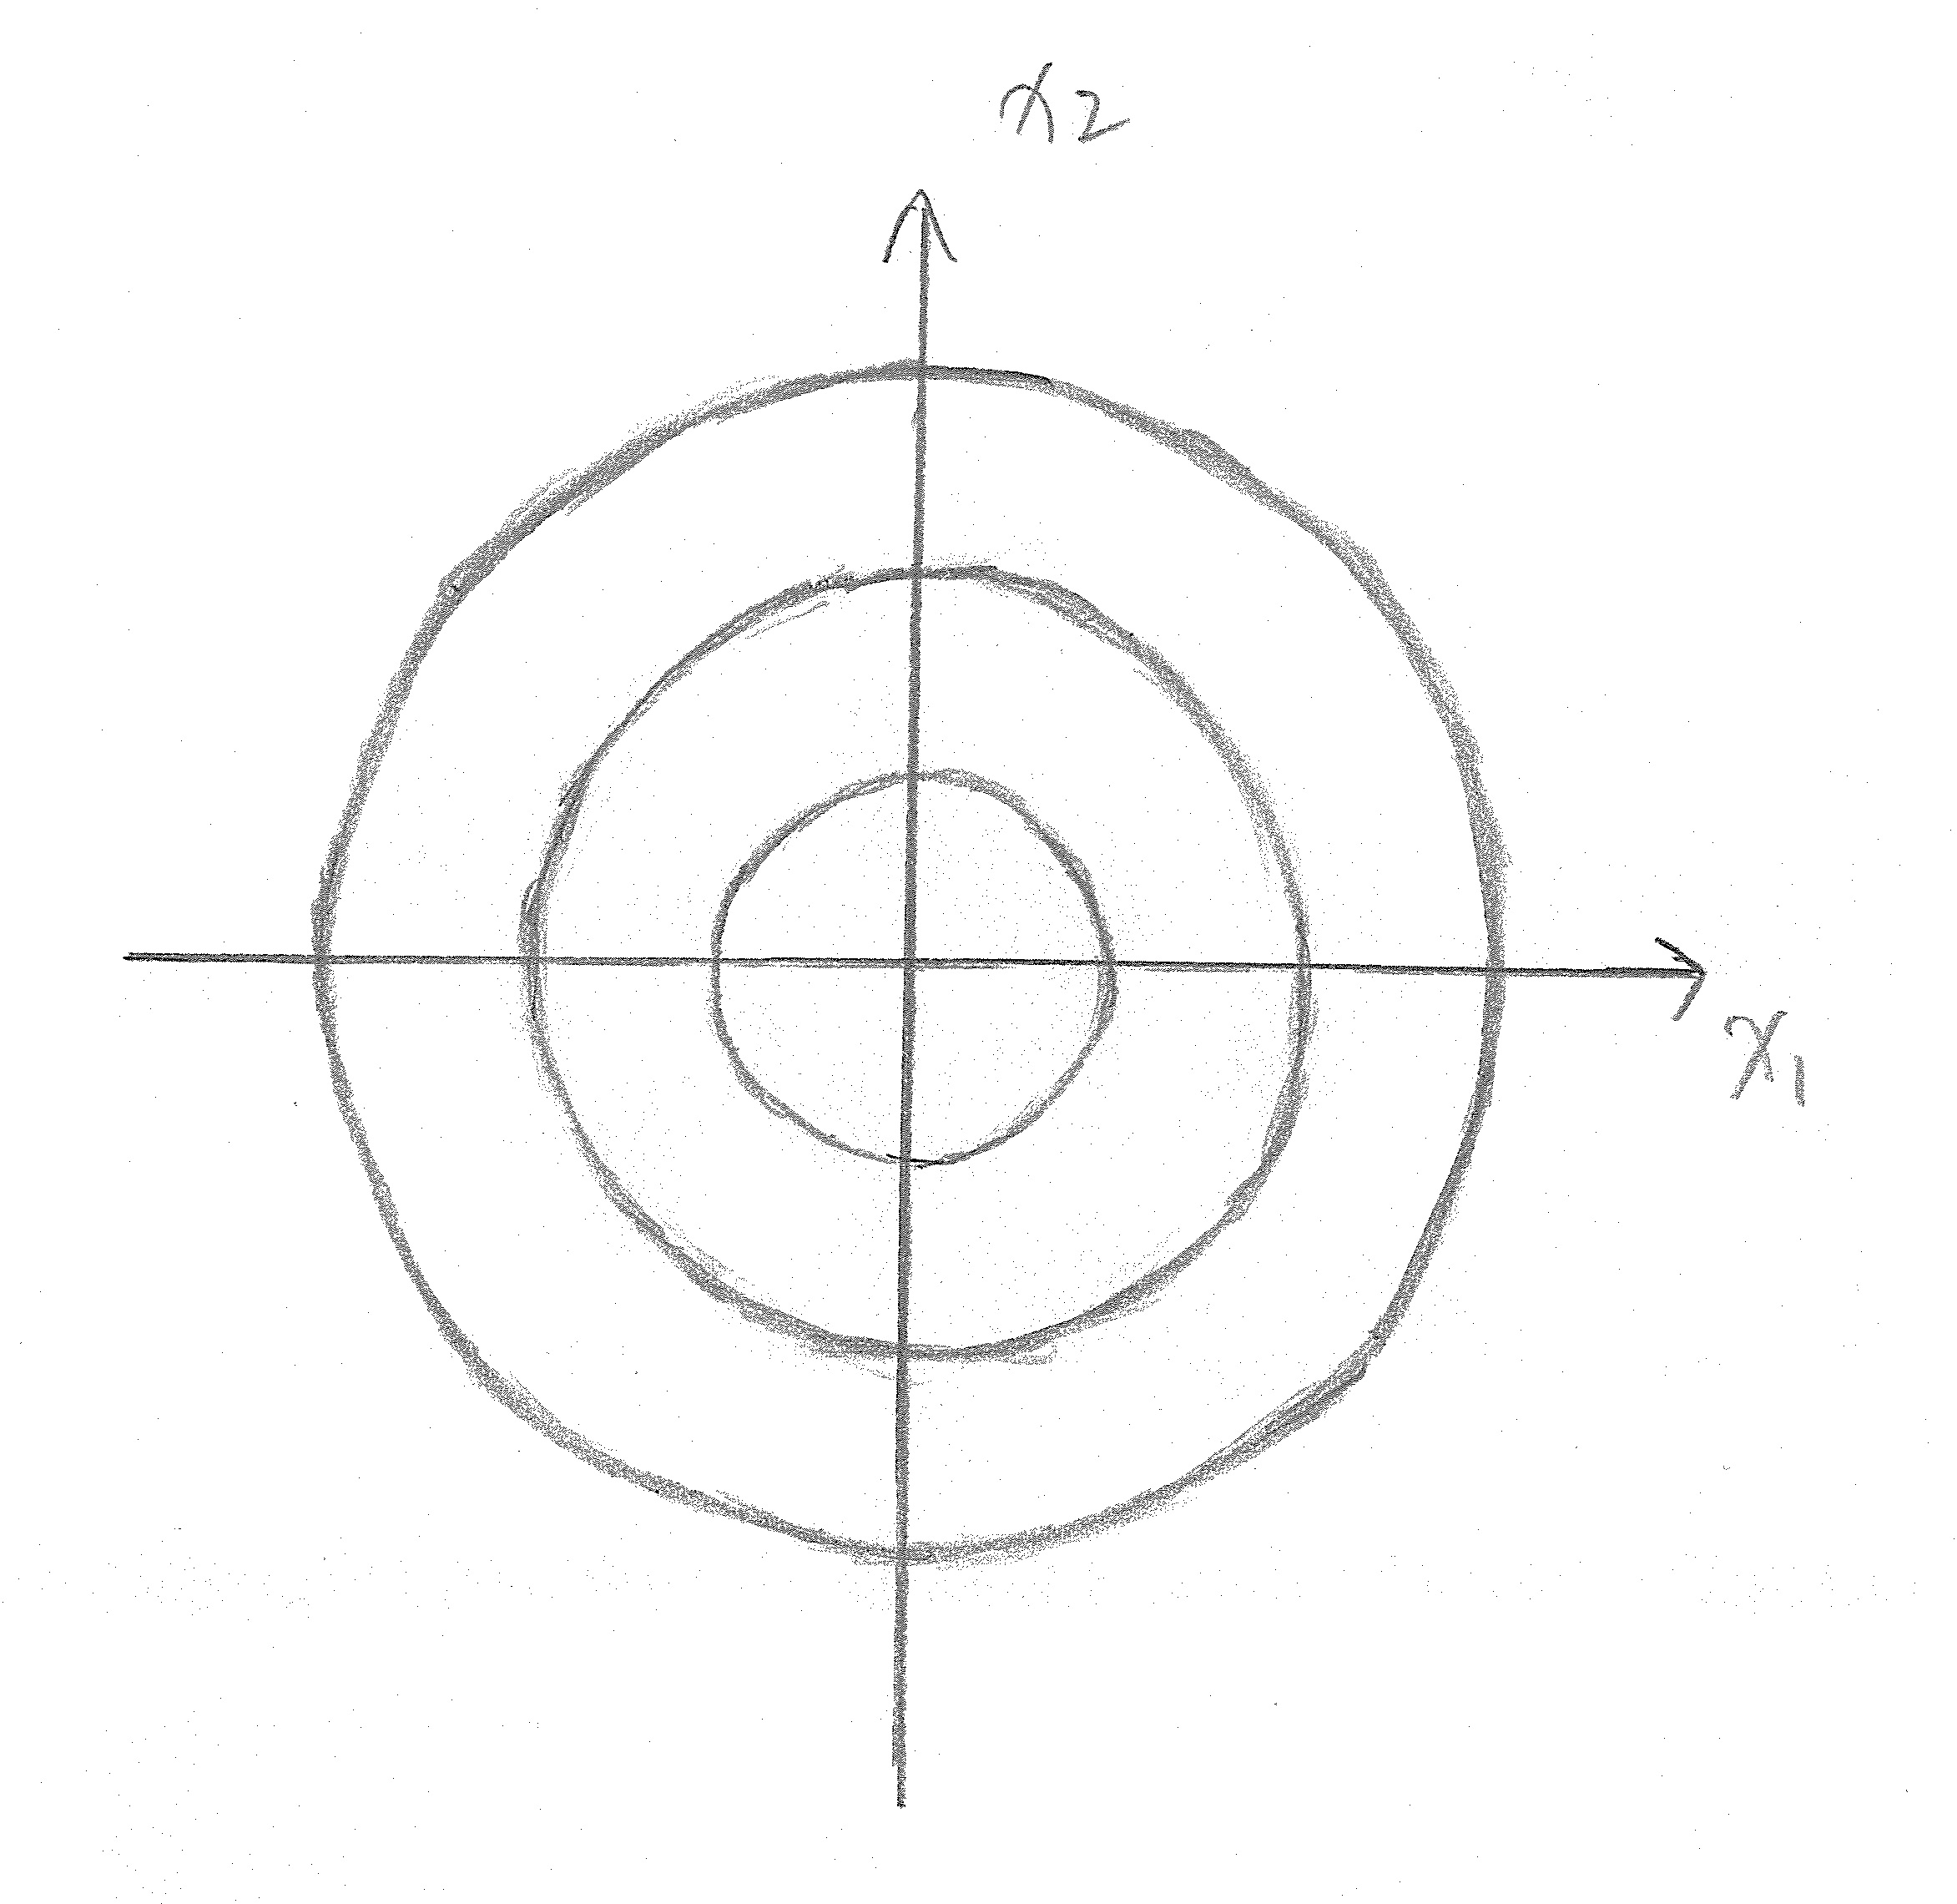
\includegraphics[width=2.1in,height=2.1in]{figures/ch02/p48-5.jpg}
		\caption{Level set 1} 
	%\label{fig:graph} 
\end{marginfigure}

\begin{marginfigure}
	\centering
	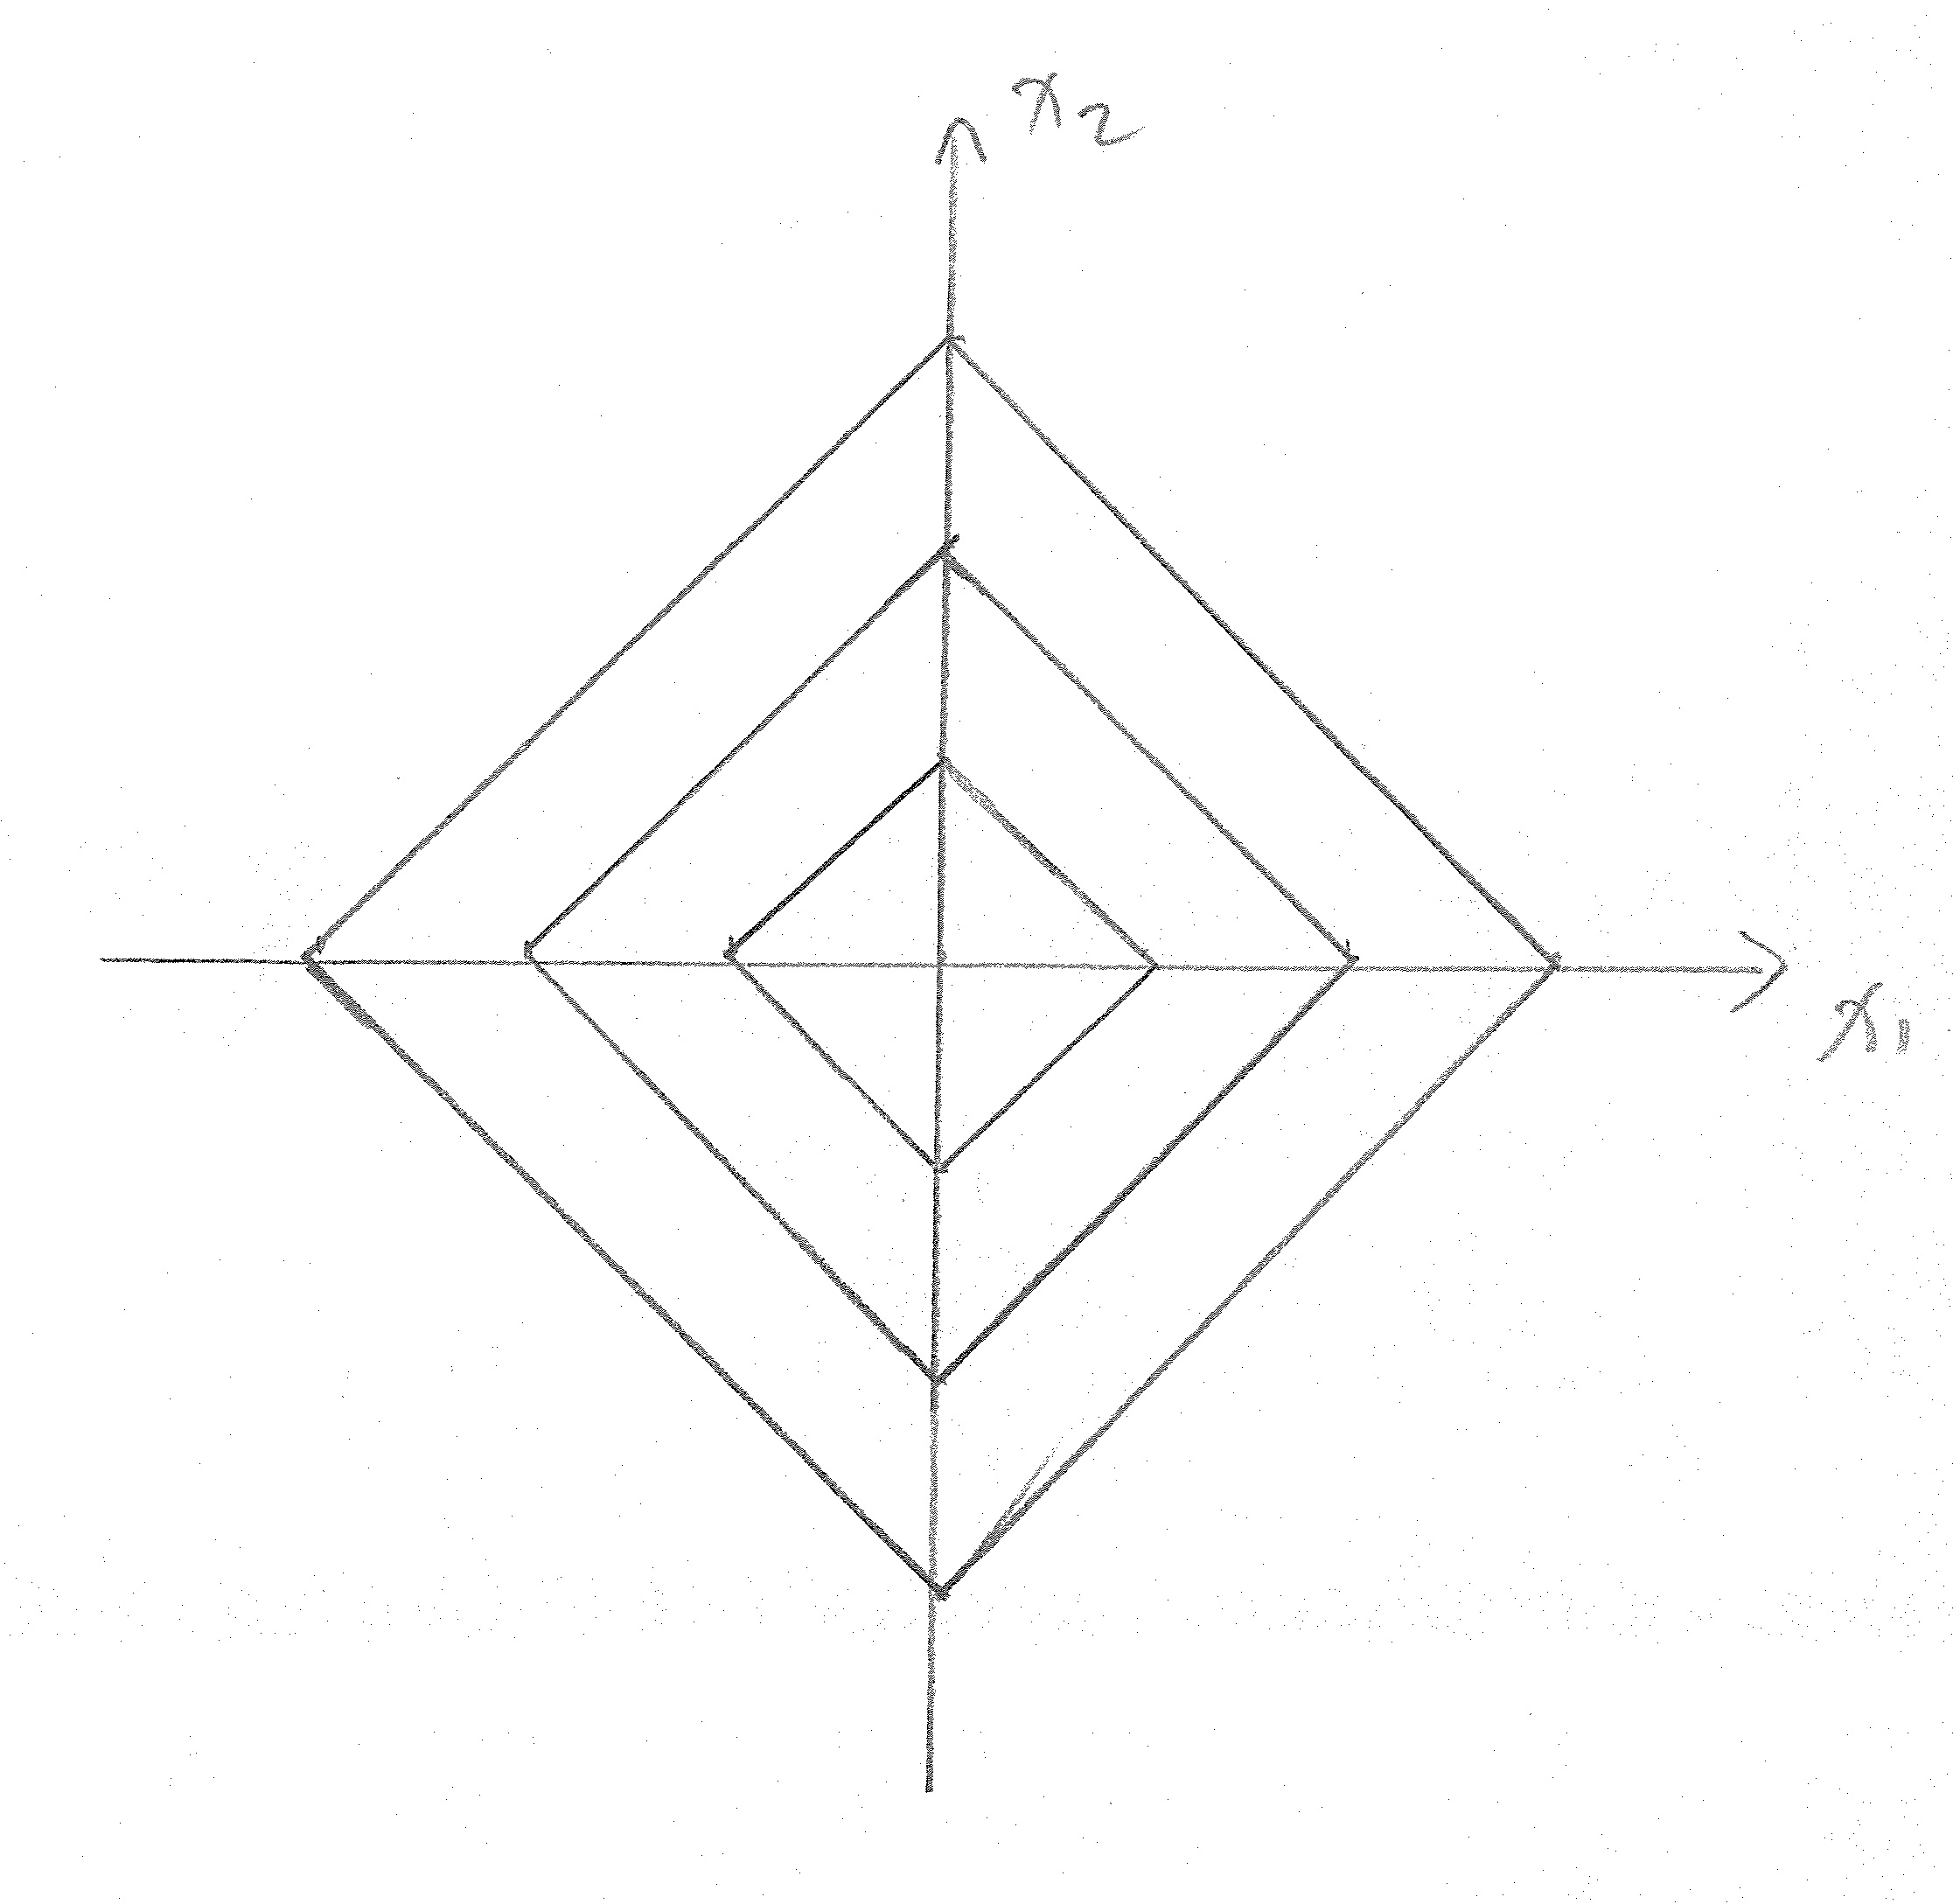
\includegraphics[width=2.1in,height=2.1in]{figures/ch02/p48-6.jpg}
	\caption{Level set 2} 
	%\label{fig:graph} 
\end{marginfigure}

\begin{marginfigure}
	\centering
	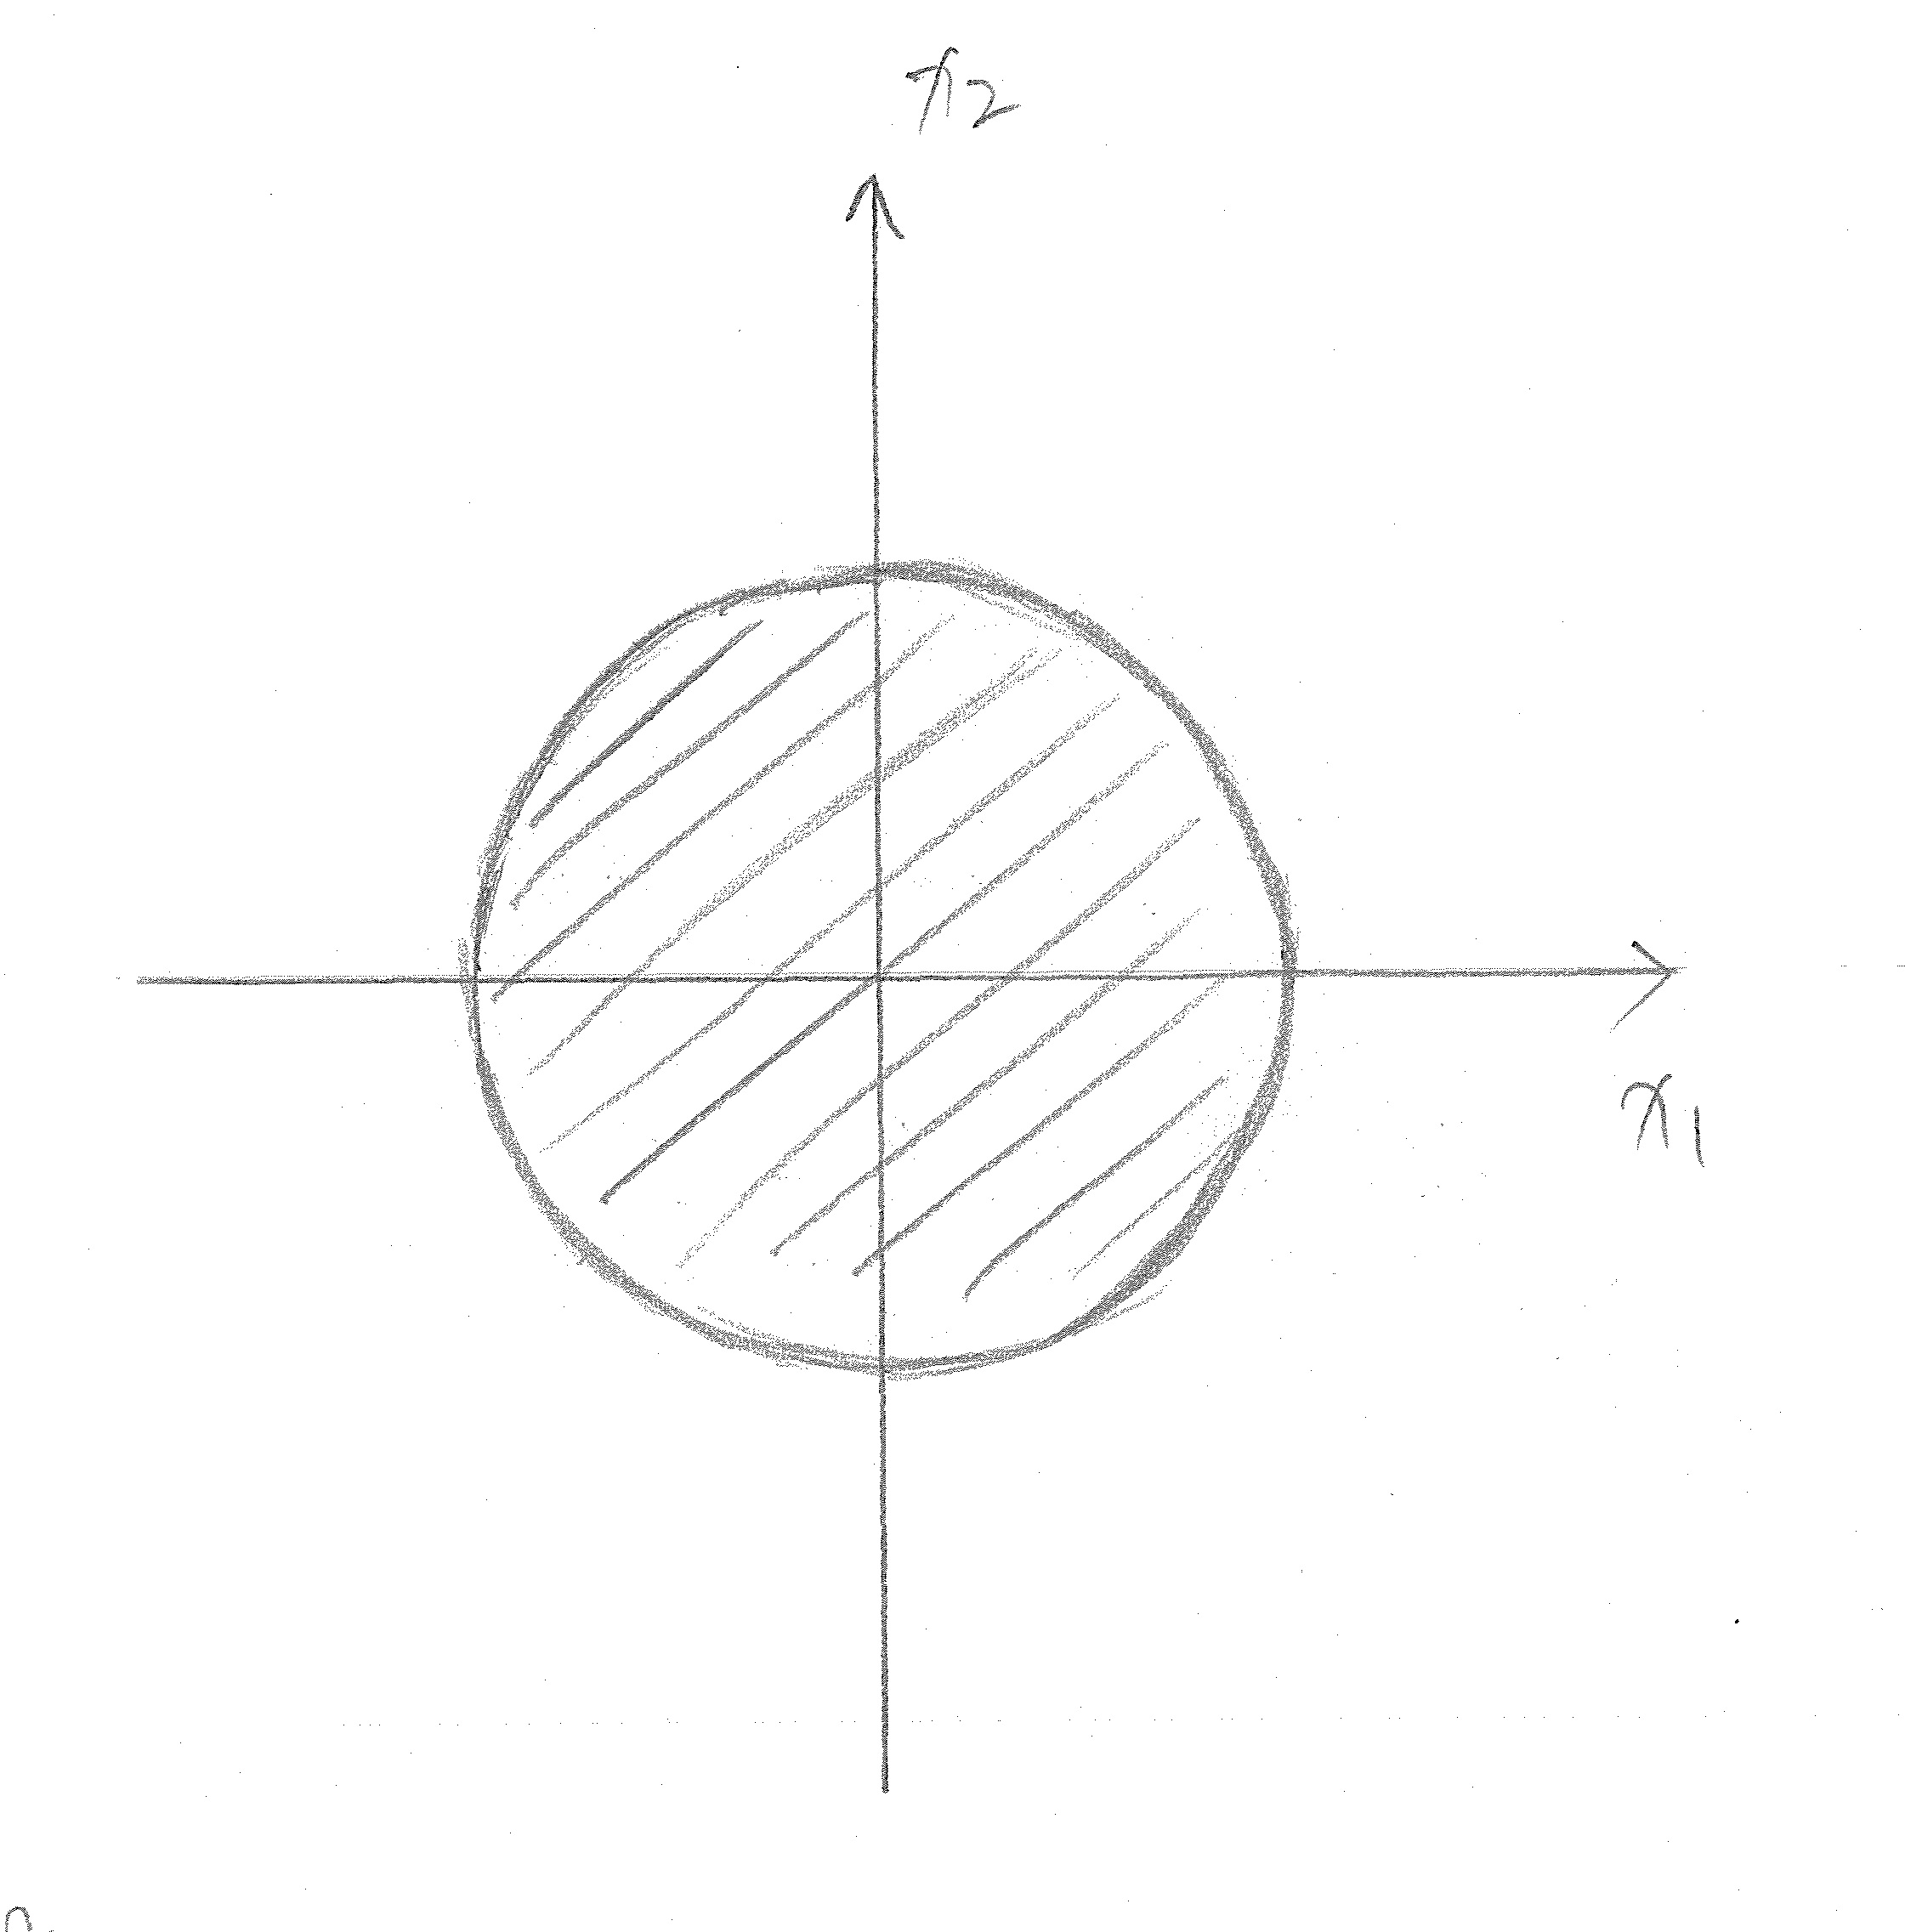
\includegraphics[width=2.1in,height=2.1in]{figures/ch02/p48-7.jpg}
	\caption{Sub-level set 1} 
	%\label{fig:graph} 
\end{marginfigure}

\begin{marginfigure}
	\centering
	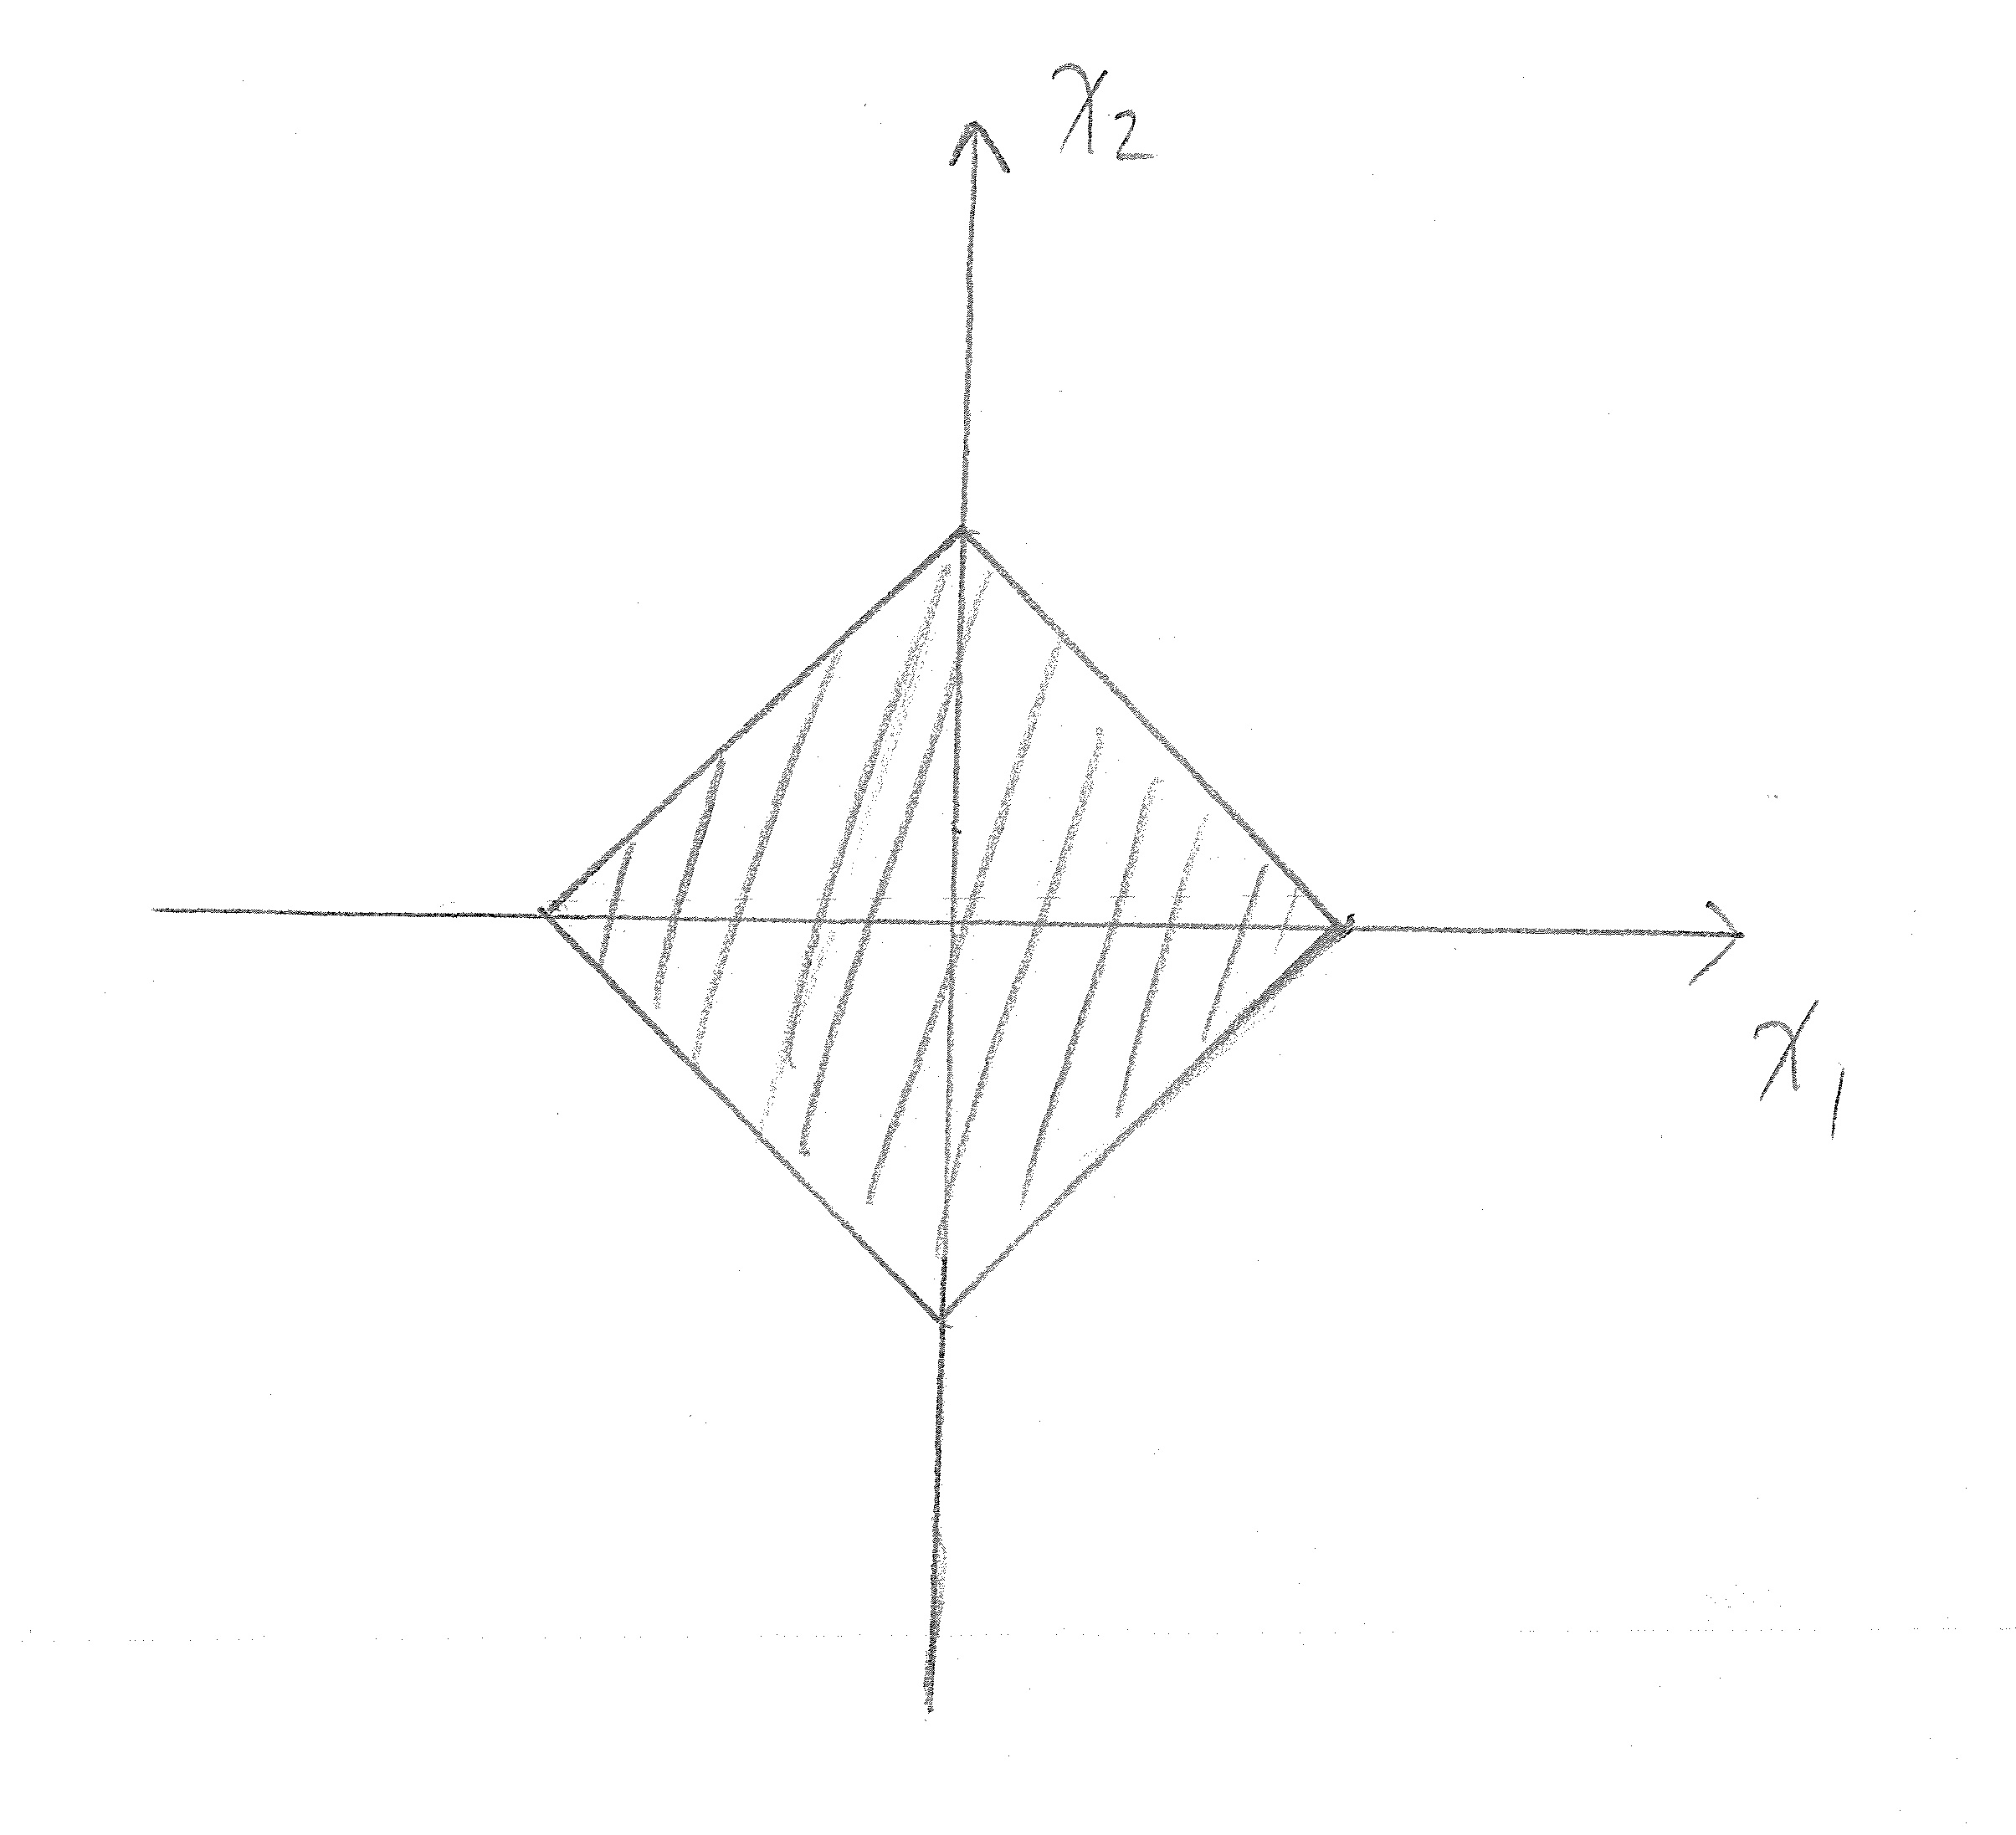
\includegraphics[width=2.1in,height=2.1in]{figures/ch02/p48-8.jpg}
	\caption{Sub-level set 2} 
	%\label{fig:graph} 
\end{marginfigure}

\vspace{0.5cm}
\textbf{Linear and affine functions}

1. A function $F:\reals^{n}\mapsto\reals$ is linear iff following two properties are satisfied

(1) "Homogeneous": $F(ax)=aF(x)$,$ \forall x\in\reals^{n}$ and $a\in\reals$

(2) "Additivity":  $F(x^{(1)}+x^{(2)})=F(x^{(1)})+F(x^{(2)})$

Put together to get 
$$F(\sum_{i\in [d]}^{}a_{i}x^{(i)})=\sum_{i\in [d]}^{}a_{i}F(x^{(i)})$$

\vspace{0.3cm}
2. A function $F:\reals^{n}\mapsto\reals$ is affine iff

Let $\overline{F}$ define pointwise as $\overline{F}=F(x)-F(0)$, $\forall x\in\reals^{n}$ is a linear function. The $F:\reals^{n}\mapsto\reals$ is affine iff there is a unique pair $(a,b)\in\reals^{n}\times\reals$ such that 
$$F(x)=a^{\trans} x+b,\  \forall x\in\reals^{n}$$

Since $F(0)=b$, this implies that any linear function can be expressed as $F(x)=a^{\trans} x=\langle a,x\rangle$ for some unique $a\in\reals^{n}$.

\vspace{0.5cm}
\textbf{Sets and linear/affine functions}

The graph of $F:\reals^{n}\mapsto\reals$ is a 

\quad- subspace of $\reals^{n+1}$ if $F$ is linear.

\quad- hyperplane of $\reals^{n+1}$ if $F$ is affine.

\vspace{0.2cm}
The epigraph of $F:\reals^{n}\mapsto\reals$ is a 

\quad- half-space of $\reals^{n+1}$ if $F$ is affine.

\quad- half-space the boarder at which includes $0\in\reals^{n+1}$ if $F$ is linear.


\begin{figure}
	\centering
	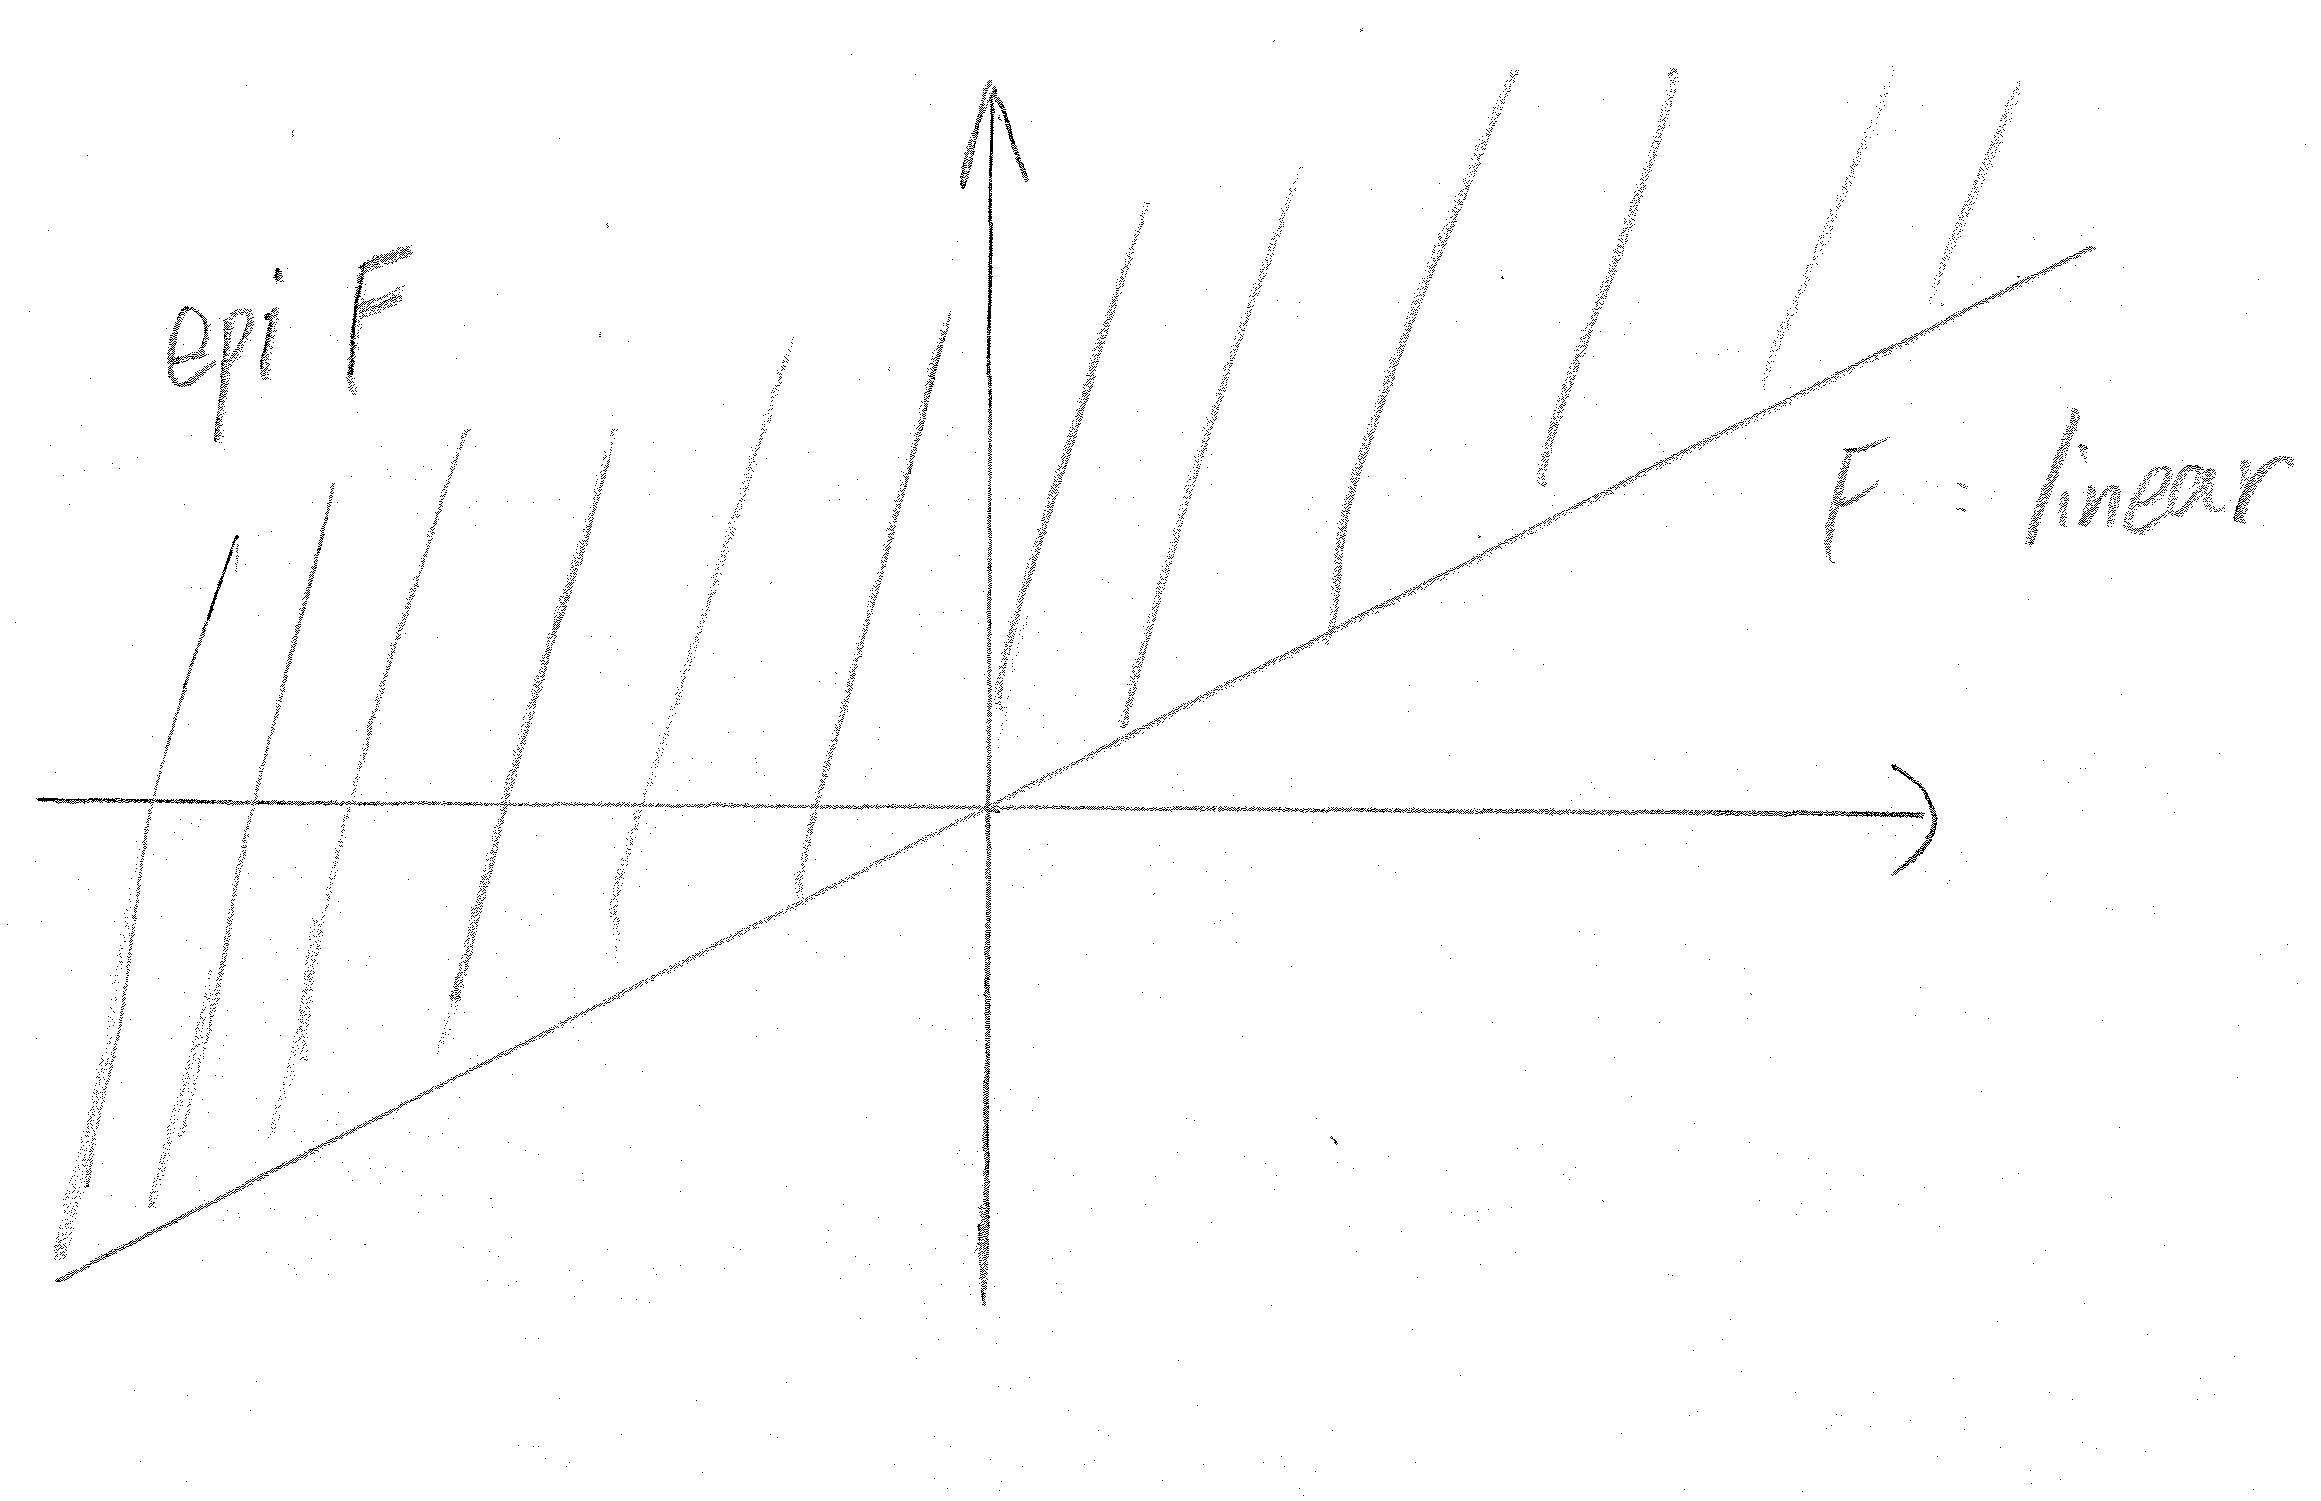
\includegraphics[width=2in,height=2in]{figures/ch02/p50-1.jpg}
	%\caption{This is an inserted JPG graphic} 
	%\label{fig:graph} 
\end{figure}

\begin{figure}
	\centering
	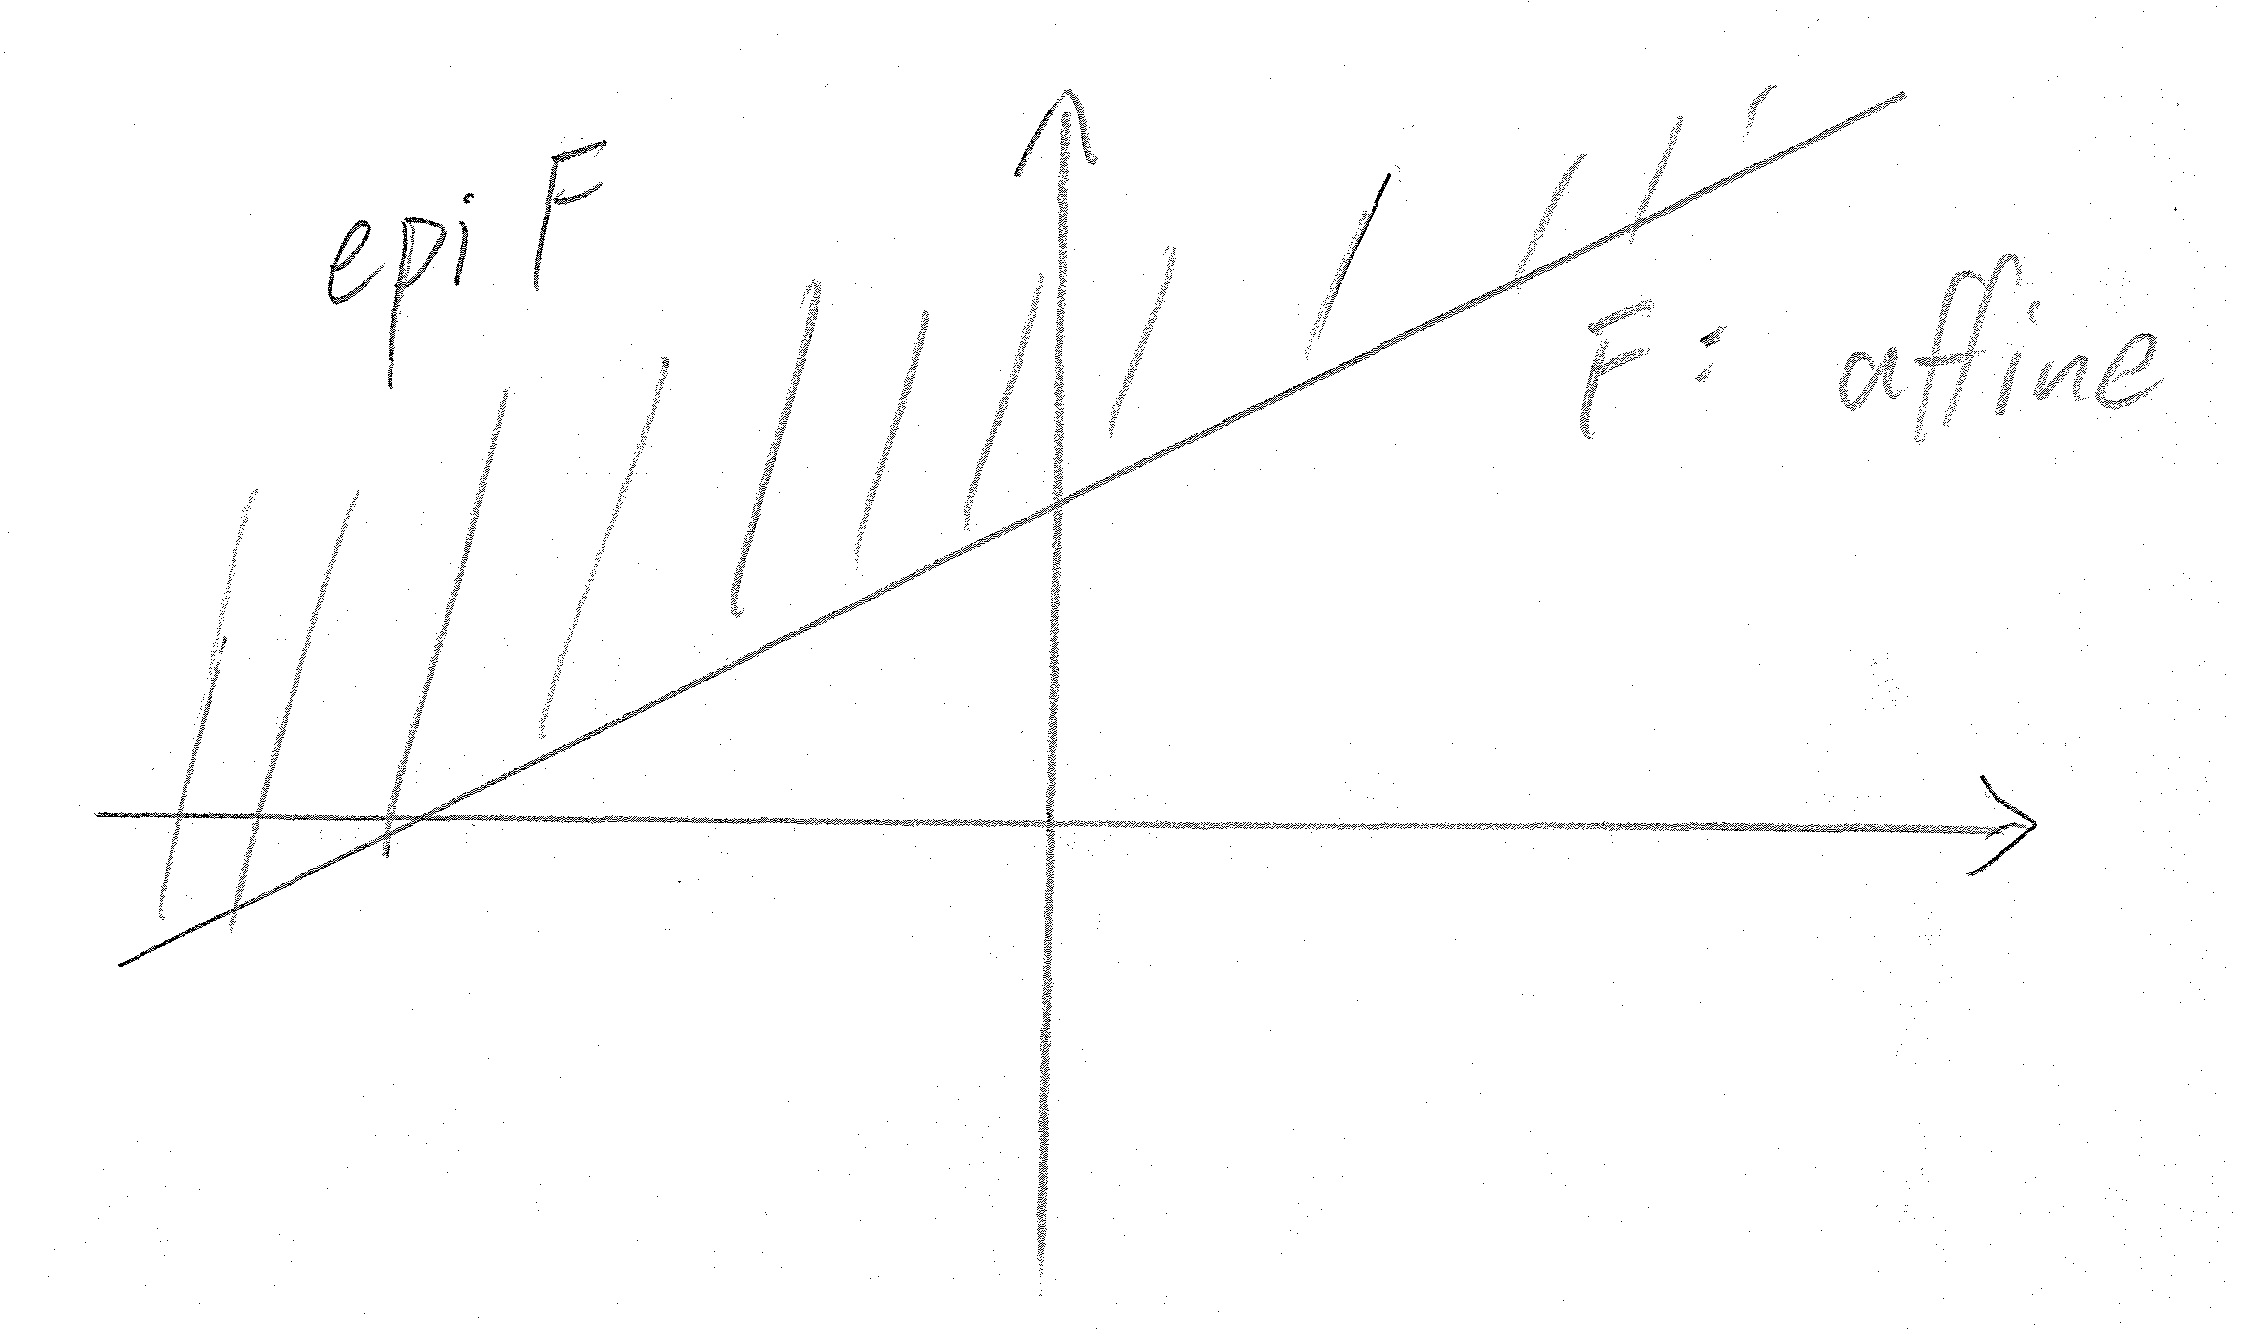
\includegraphics[width=2.1in,height=2.1in]{figures/ch02/p50-2.jpg}
	%\caption{This is an inserted JPG graphic} 
	%\label{fig:graph} 
\end{figure}


Similar statements hold for level sets and sub-level sets in $\reals^{n}$, e.g., level sets of a linear function $F:\reals^{2}\mapsto\reals$ are affine sets in $\reals^{2}$

\begin{figure}
	\centering
	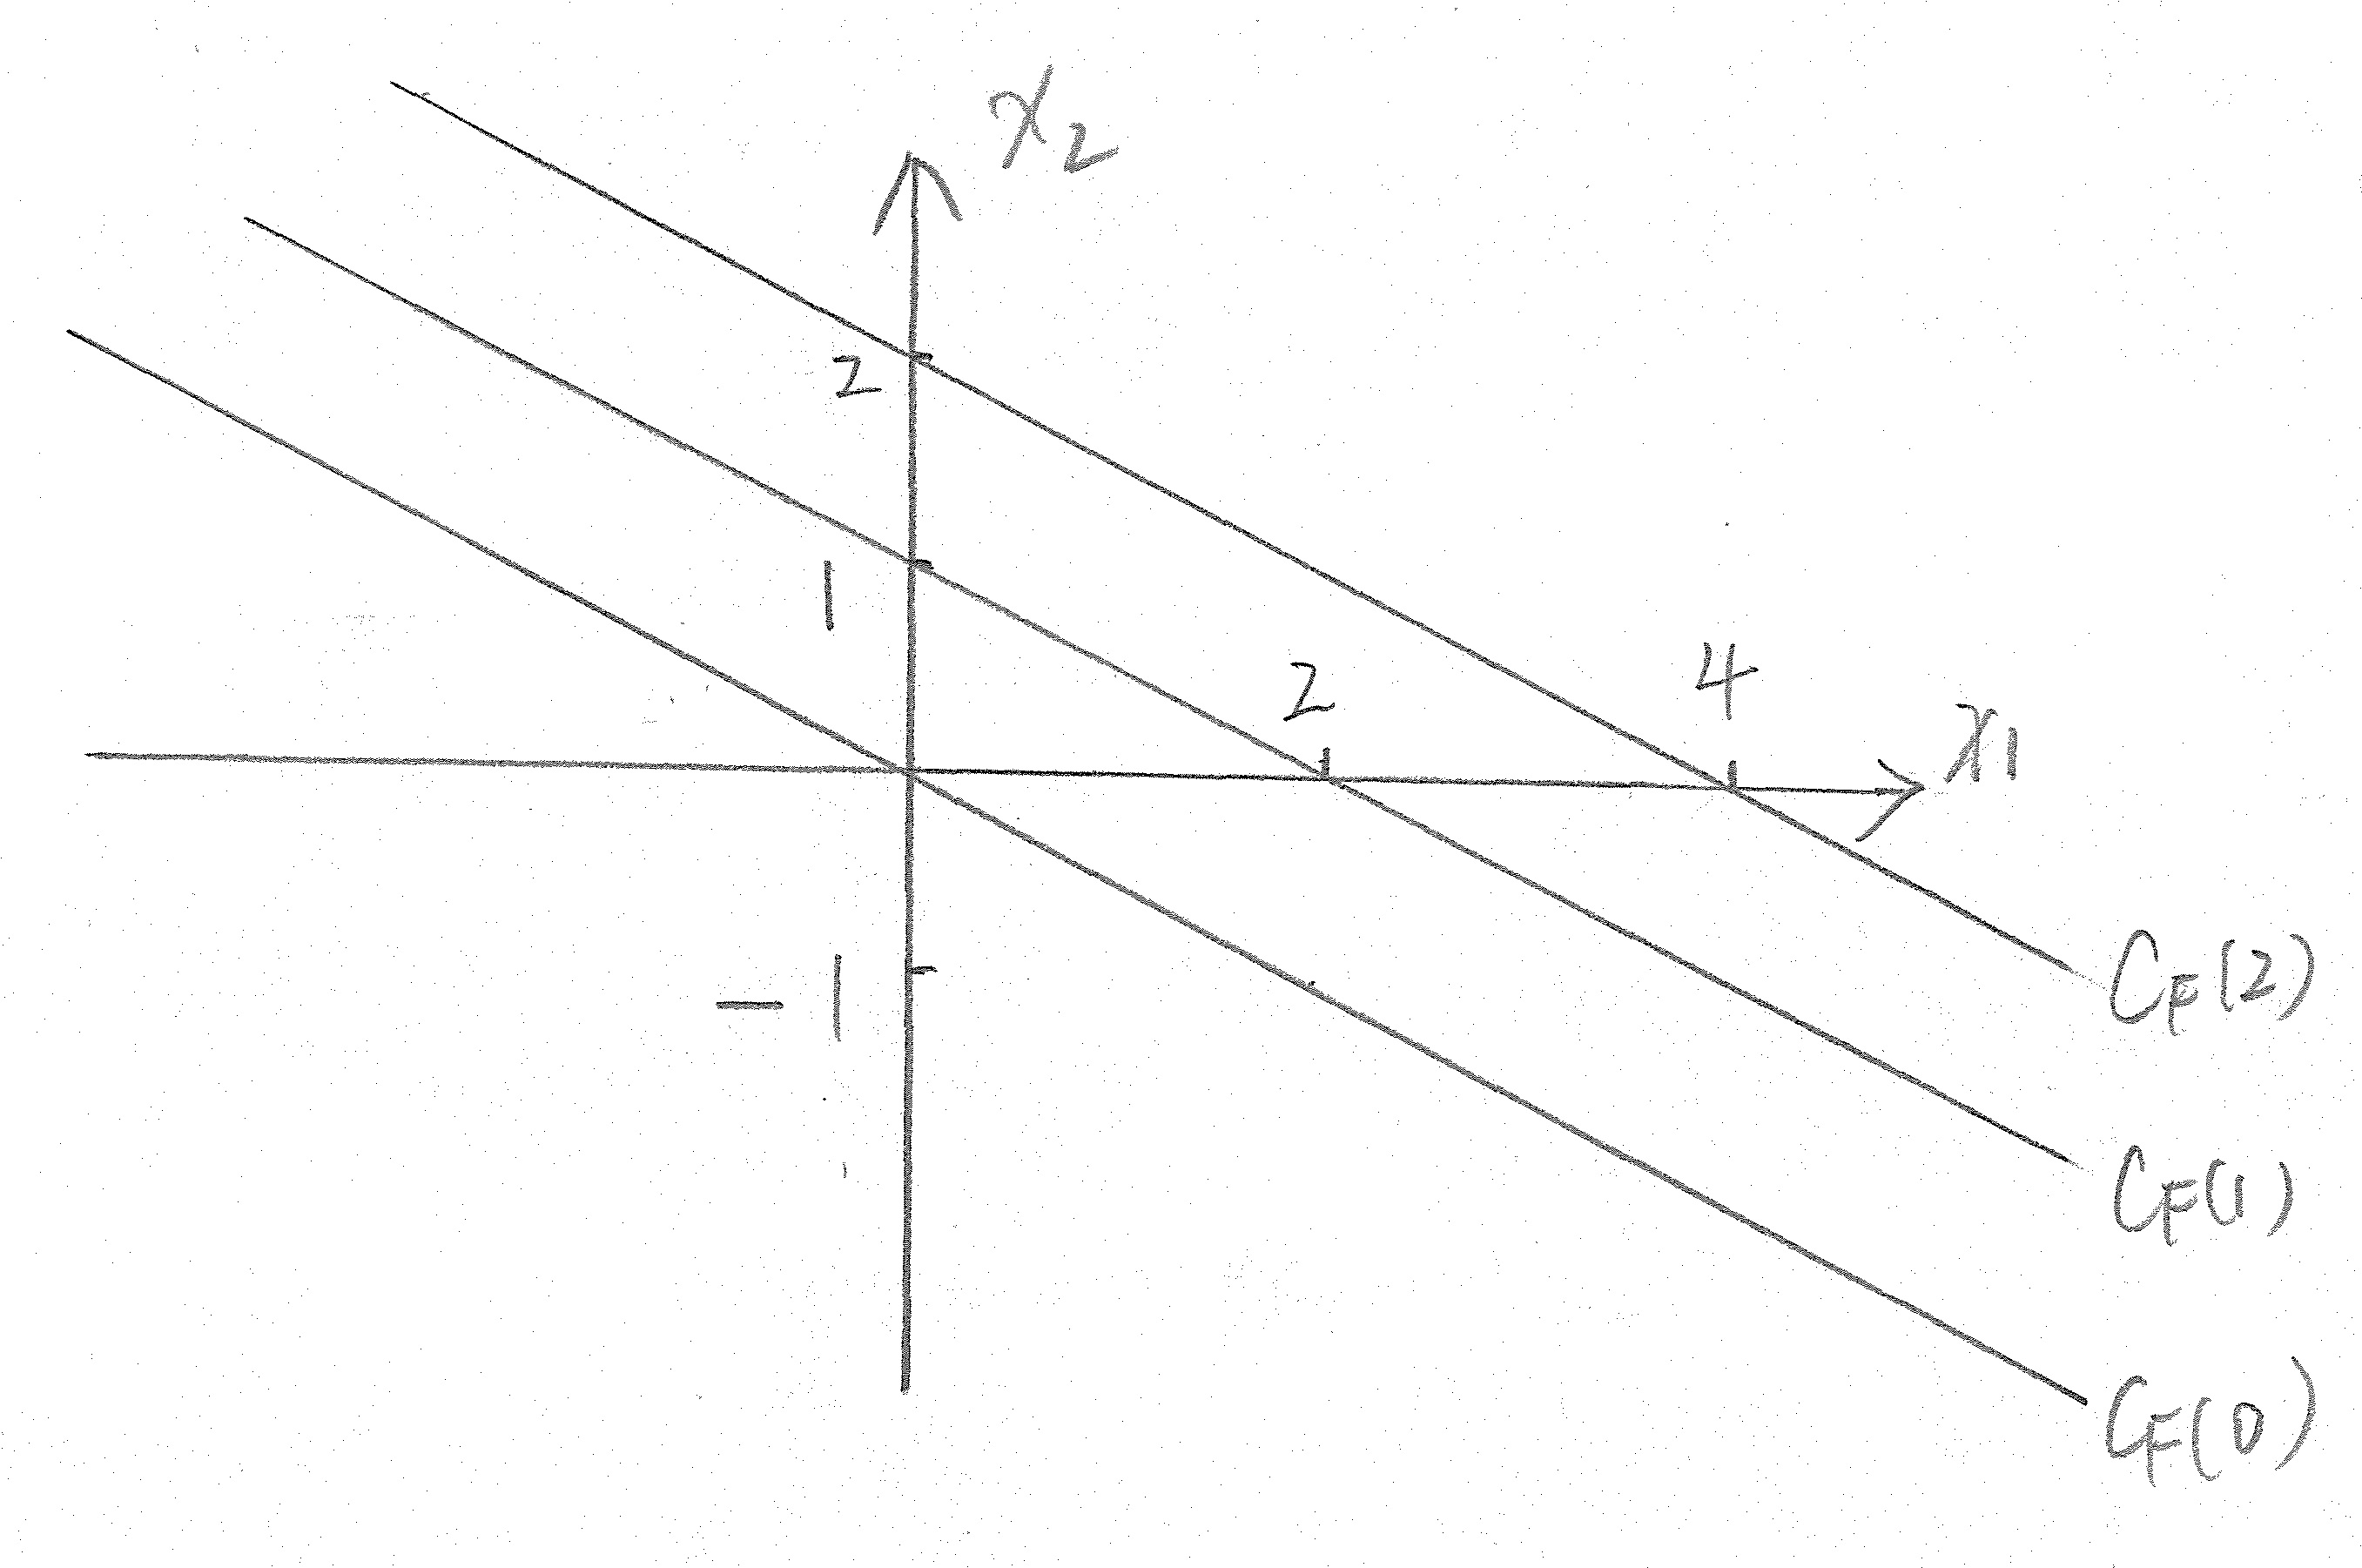
\includegraphics[width=2.1in,height=2.1in]{figures/ch02/p50-3.jpg}
	%\caption{This is an inserted JPG graphic} 
	%\label{fig:graph} 
\end{figure}

\vspace{0.3cm}
Definition of a hyperplane:
$$\mathcal{H}=\{z\in\reals^{n}|a^{\trans} z=b,a\in\reals^{n}, b\in\reals \}$$

\begin{marginfigure}
	\centering
	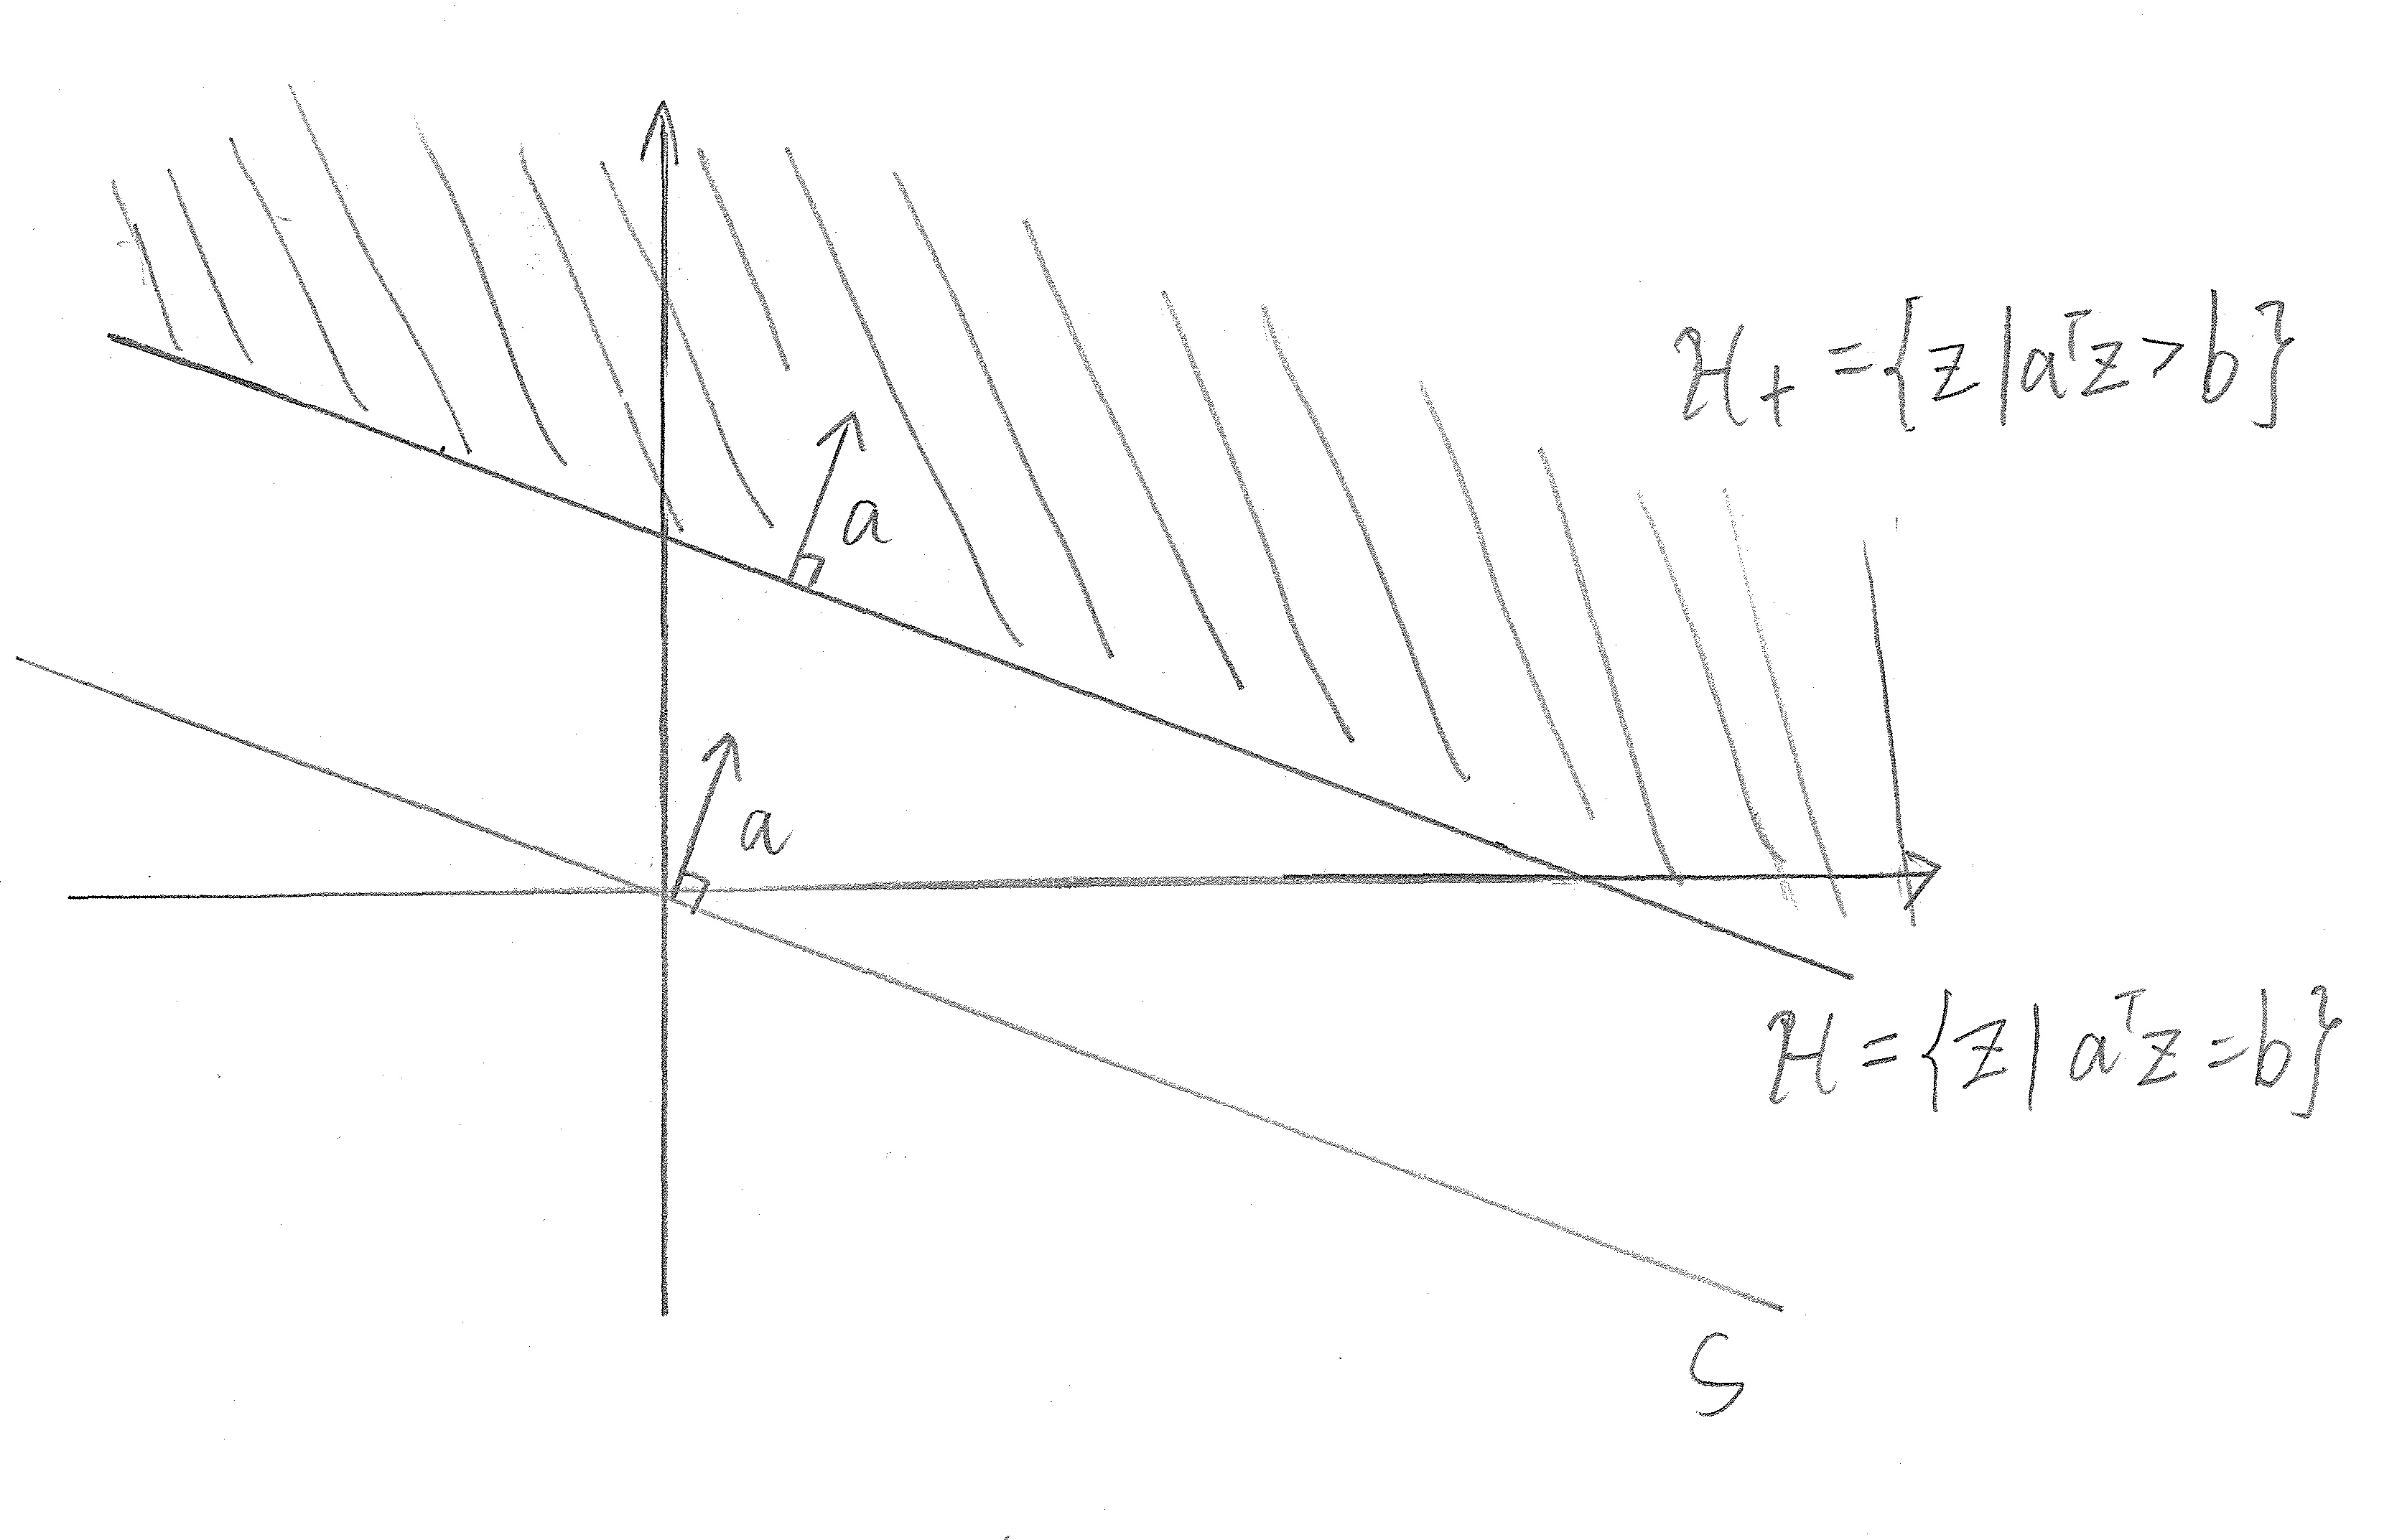
\includegraphics[width=2.1in,height=2.1in]{figures/ch02/p53.jpg}
	%\caption{This is an inserted JPG graphic} 
	\label{fig:graph} 
\end{marginfigure}

Definition of Half-spaces: are on one side or other of a hyperplane(see the r.h.s for a graph of $\mathcal{H}_{+}$),
$$\mathcal{H}_{+}=\{z\in\reals^{n}|a^{\trans} z>b\}$$
$$\mathcal{H}_{-}=\{z\in\reals^{n}|a^{\trans} z\leq b\}$$



\vspace{0.5cm}

\textbf{Gradient}

The gradient $\nabla F$ of $F:\reals^{n}\mapsto\reals$ is the vector of partial derivatives
$$\nabla F= 
\left[ 
\begin{array}{c} 
\frac{\partial F(x)}{\partial x_{1}} \\
\frac{\partial F(x)}{\partial x_{2}} \\
\vdots \\
\frac{\partial F(x)}{\partial x_{n}}
\end{array}
\right],
\ \text{where}\ x= 
\left[ 
\begin{array}{c} 
x_{1} \\
x_{2} \\
\vdots \\
x_{n}
\end{array}
\right]$$

Sometime  we need to consider compound function, and thus we need chain rule for gradients. Says, $g:\reals^{n}\mapsto\reals^{m}$ and $F:\reals^{m}\mapsto\reals$, both $F$ and $g$ are differentiable and we want $\nabla\Phi (x)$, where $\Phi (x)=F(g(x))$. In this case we have
$$
\nabla \phi (x)
=
\left[\begin{matrix}
	\frac{\partial \phi (x)}{\partial x_{1}}\\
	\vdots\\
	\vdots\\
	\frac{\partial \phi (x)}{\partial x_{n}}\\
\end{matrix}\right]
=
\left[\begin{matrix}
	\frac{\partial g_{1}(x)}{\partial x_{1}}&\frac{\partial g_{2}(x)}{\partial x_{1}}&\cdots&\frac{\partial g_{m}(x)}{\partial x_{1}}\\
	\frac{\partial g_{1}(x)}{\partial x_{2}}&\ddots & &\vdots\\
	\vdots& &\ddots &\vdots \\
	\frac{\partial g_{1}(x)}{\partial x_{n}}&\cdots&\cdots&\frac{\partial g_{m}(x)}{\partial x_{n}}
\end{matrix}\right]
\nabla F\left(g(x)\right)
$$

Example 

Let $g:\reals^{4}\mapsto\reals^{3}$ and $F:\reals^{3}\mapsto\reals$, both $F$ and $g$ are differentiable and we want to find $\nabla\Phi (x)$. To simplify, we let the function $g$ and $F$ takes the form,

$g(x)=Ax+b$, where $A$ is an $3$ by $4$ matrix, $x$ is a $4$ dimensions vector,  and $b$ is $3$ dimensions vector, so function $g$ maps $\reals^{4}$ to $\reals^{3}$.
 

$F(x)=Cx$, where $C$ is an $1$ by $3$ matrix and the input $x$ is a $3$ dimensions vector, so function $F$ maps $\reals^{3}$ to $\reals$.

Hence, the gradient of $\Phi (x)$ is
\begin{align*}
\nabla \phi (x) &=
\left[\begin{matrix}
\frac{\partial \phi (x)}{\partial x_{1}}\\
\frac{\partial \phi (x)}{\partial x_{2}}\\
\frac{\partial \phi (x)}{\partial x_{13}}\\
\frac{\partial \phi (x)}{\partial x_{4}}\\
\end{matrix}\right]\\
&=
\left[\begin{matrix}
\frac{\partial g_{1}(x)}{\partial x_{1}}&\frac{\partial g_{2}(x)}{\partial x_{1}}&\frac{\partial g_{3}(x)}{\partial x_{1}}\\
\frac{\partial g_{1}(x)}{\partial x_{2}}&\frac{\partial g_{2}(x)}{\partial x_{2}}&\frac{\partial g_{3}(x)}{\partial x_{2}}\\
\frac{\partial g_{1}(x)}{\partial x_{3}}&\frac{\partial g_{2}(x)}{\partial x_{3}}&\frac{\partial g_{3}(x)}{\partial x_{3}}\\
\frac{\partial g_{1}(x)}{\partial x_{4}}&\frac{\partial g_{2}(x)}{\partial x_{4}}&\frac{\partial g_{3}(x)}{\partial x_{4}}
\end{matrix}\right]
\left[\begin{matrix}
\frac{\partial \phi (x)}{\partial g_{1}}\\
\frac{\partial \phi (x)}{\partial g_{2}}\\
\frac{\partial \phi (x)}{\partial g_{3}}\\
\end{matrix}\right]\\
&=
\left[\begin{matrix}
a_{11}&a_{21}&a_{31}\\
a_{12}&a_{22}&a_{32}\\
a_{13}&a_{23}&a_{33}\\
a_{14}&a_{24}&a_{34}\\
\end{matrix}\right]
\left[\begin{matrix}
c_{11}\\
c_{12}\\
c_{13}\\
\end{matrix}\right]\\
&=
A^{\trans}C^{\trans}\\
\end{align*}

\textbf{Affine approximations}

Consider the Taylor series for $F\colon \mathbb{R}^n \to \mathbb{R}$.

$$F(x) = F(x_0) + \nabla F(x_0)^{T} (x - x_0) + \varepsilon (x) $$


Example 1. $F(x) = 2 x_1^2 + x_2^2$

$$F(x) \cong F(x^{(0)}) + \nabla F(x^{(0)})^{T} (x - x^{(0)})
\left. \nabla F(x) \right|_{x} \qquad (*)$$

$$\nabla F(x) = \begin{bmatrix} 4x_1\\ 2x_2\\ \end{bmatrix}$$

\begin{displaymath}
\nabla F \left( \begin{bmatrix} 0\\ 0\\ \end{bmatrix} \right)  =
\begin{bmatrix} 0\\ 0\\ \end{bmatrix}
\end{displaymath}

\begin{displaymath}
\nabla F \left( \begin{bmatrix} 1\\ 0\\ \end{bmatrix} \right)  =
\begin{bmatrix} 4\\ 0\\ \end{bmatrix}
\end{displaymath}

\begin{displaymath}
\nabla F \left( \begin{bmatrix} 0\\ 1\\ \end{bmatrix} \right)  =
\begin{bmatrix} 0\\ 2\\ \end{bmatrix}
\end{displaymath}


\begin{figure}
	\centering
	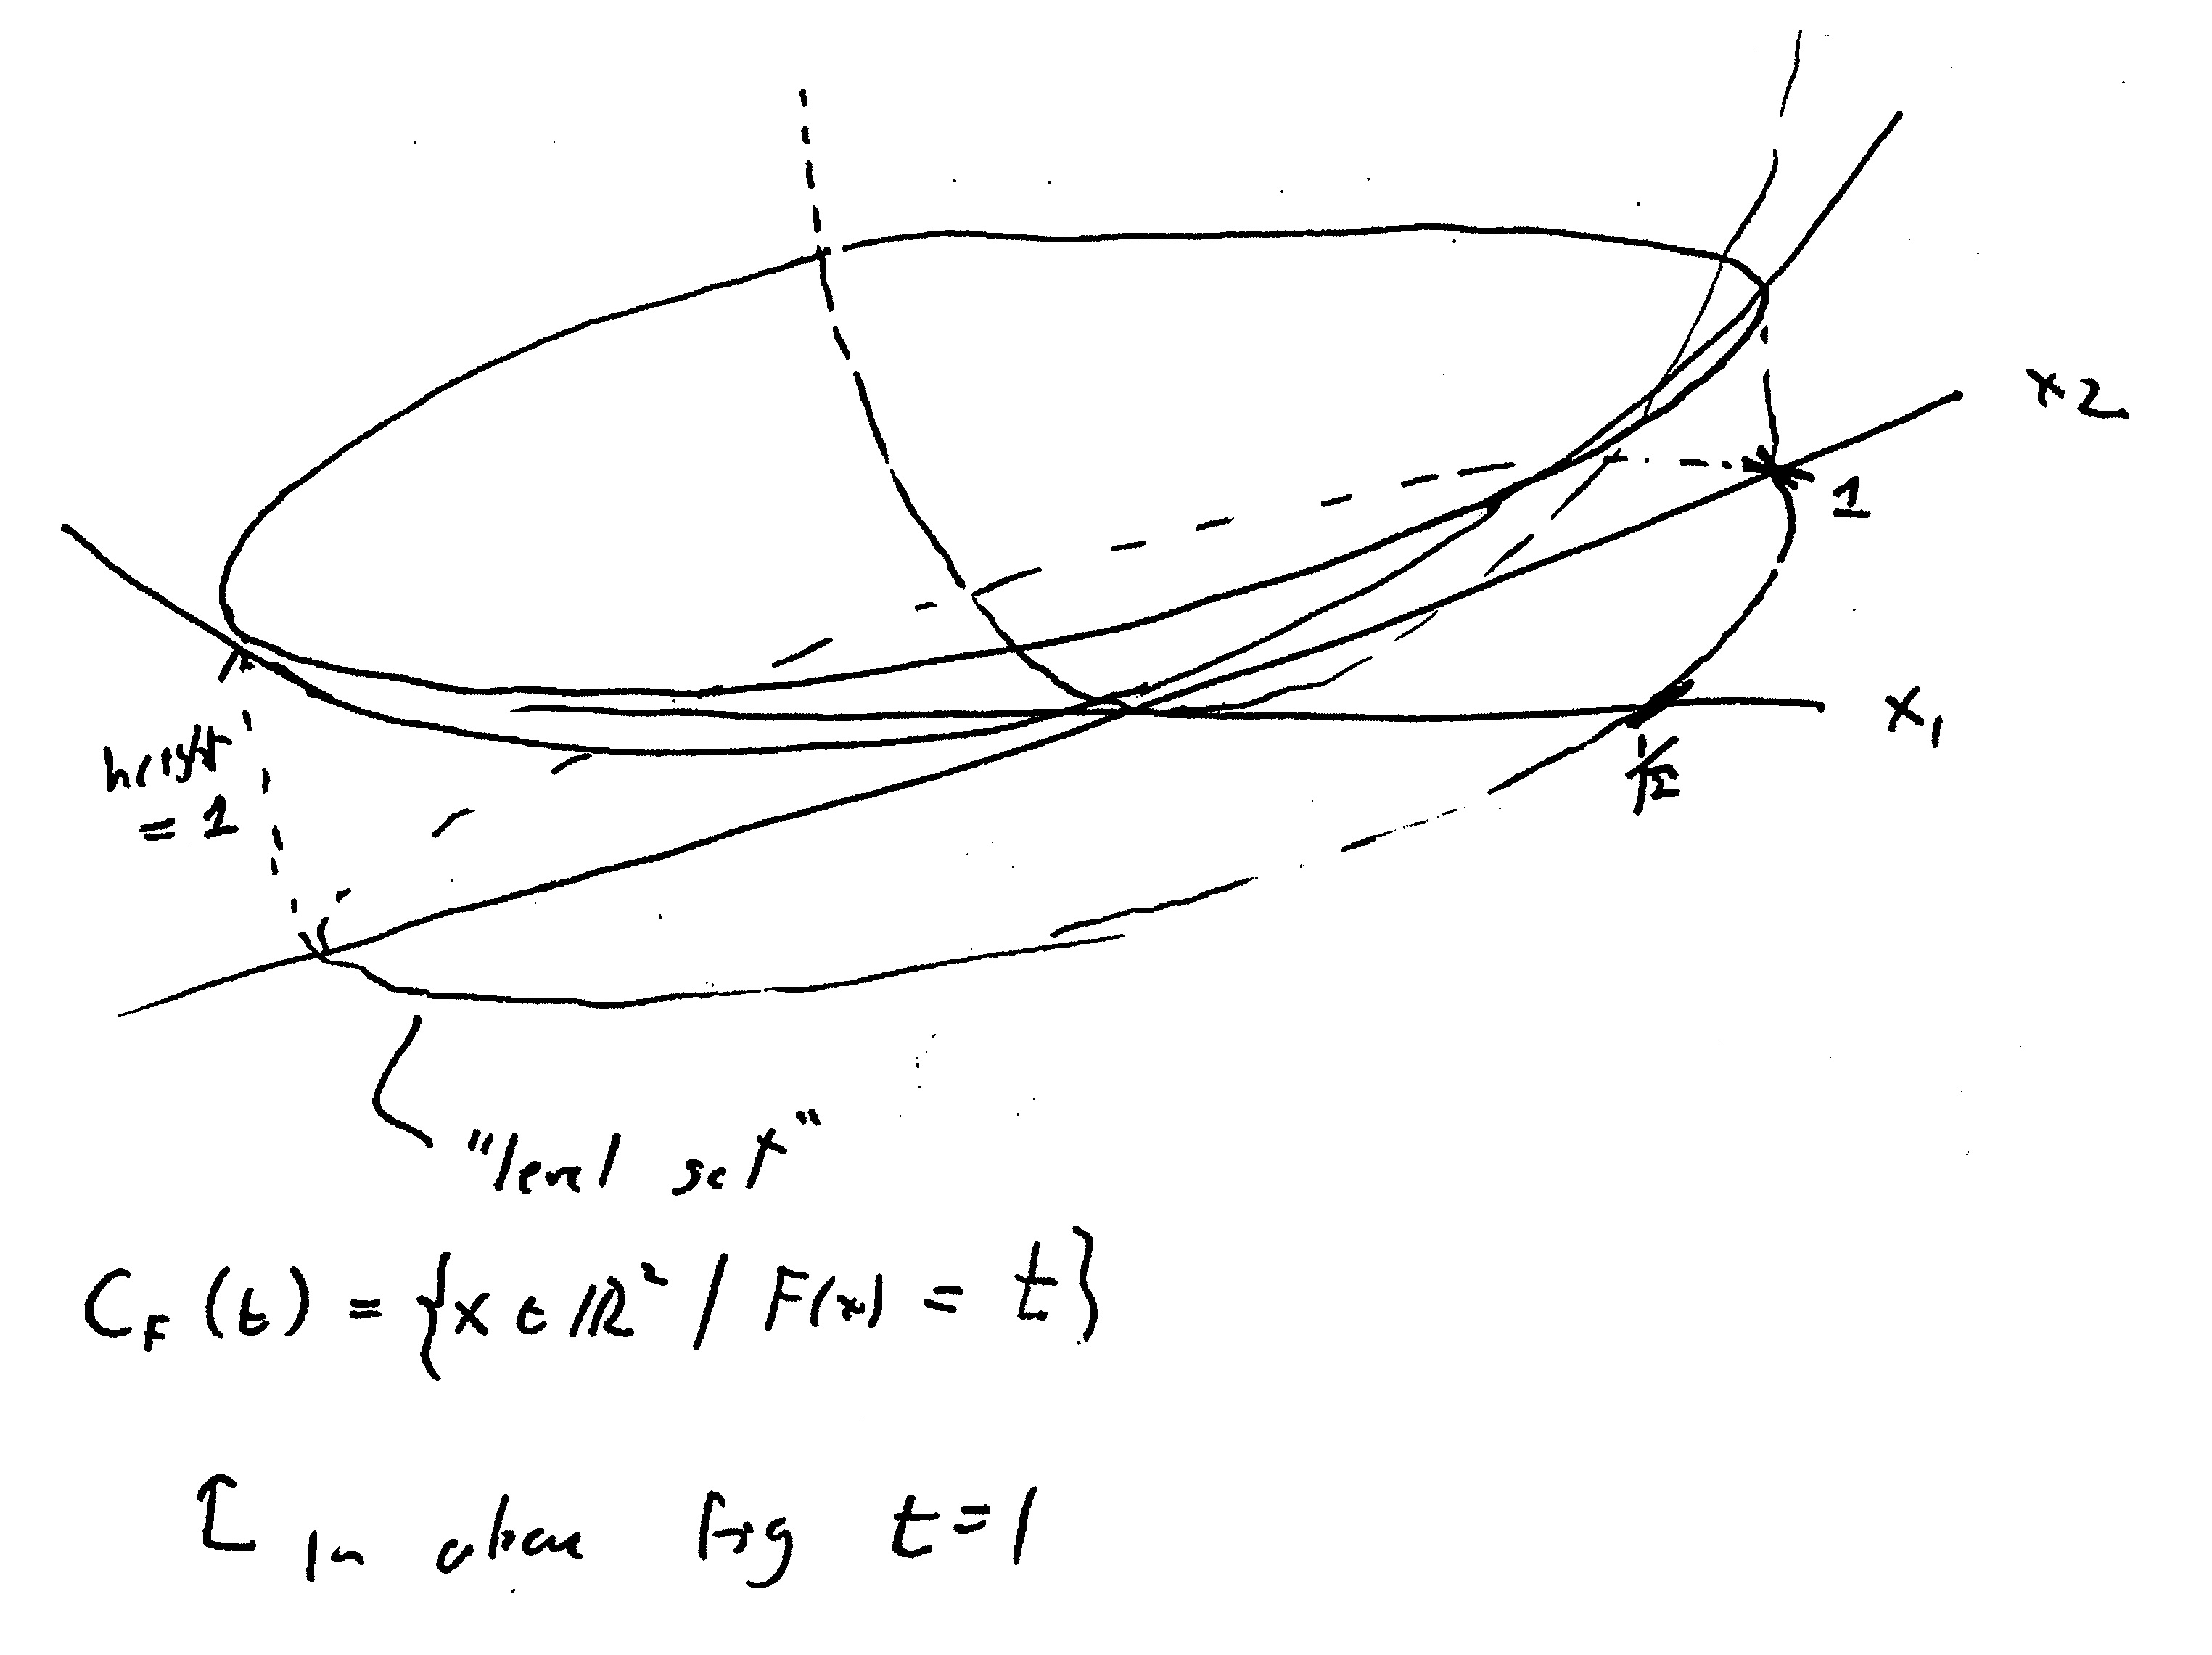
\includegraphics[width=3in,height=3in]{figures/ch02/p59.jpg}
	%\caption{This is an inserted JPG graphic} 
	%\label{fig:graph} 
\end{figure}

Let's sketch the "level set" in 2-D, 

\begin{figure}
	\centering
	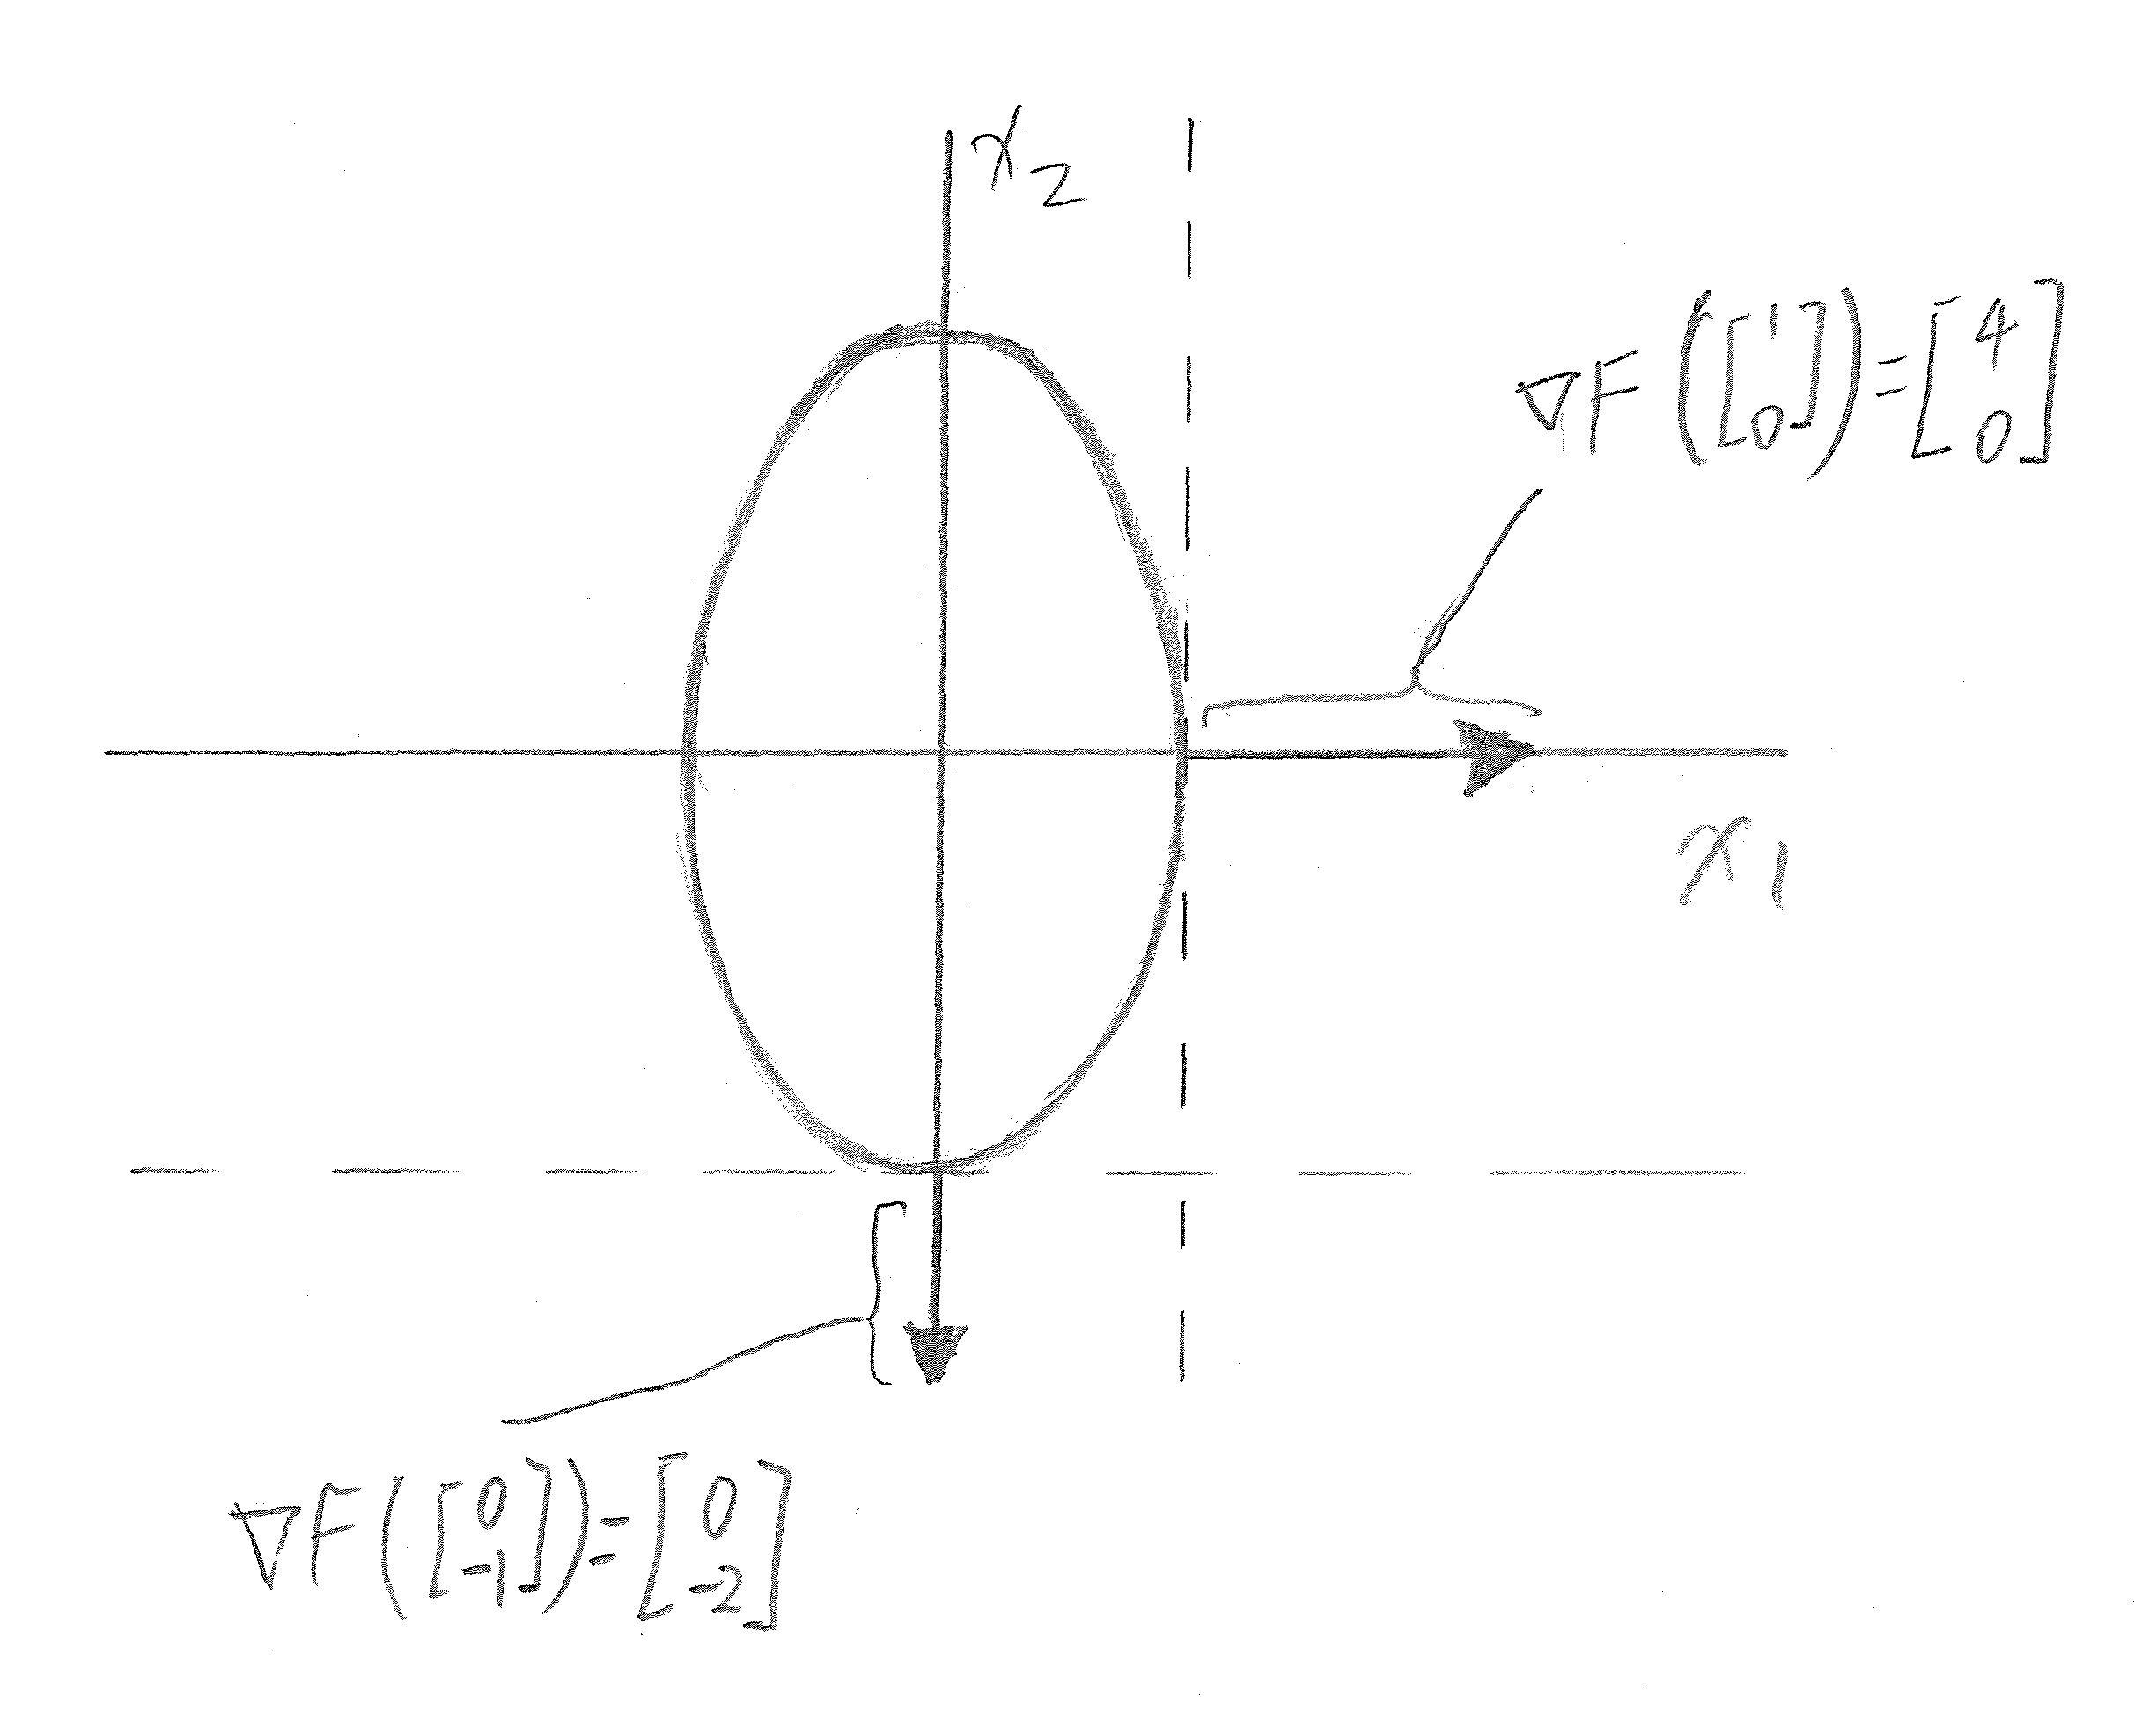
\includegraphics[width=2.1in,height=2.1in]{figures/ch02/p60-1.jpg}
	%\caption{This is an inserted JPG graphic} 
	%\label{fig:graph} 
\end{figure}

\begin{displaymath}
\nabla F \left( \begin{bmatrix} 1\\ 0\\ \end{bmatrix} \right)  =
\begin{bmatrix} 4\\ 0\\ \end{bmatrix}
\end{displaymath}

\begin{displaymath}
\nabla F \left( \begin{bmatrix} 0\\ -1\\ \end{bmatrix} \right)  =
\begin{bmatrix} 0\\ -2\\ \end{bmatrix}
\end{displaymath}

Let's visualize the set such that the increment in $(*)$ is, to first order, constant. That is, which $x \in \mathbb{R}^2$ satisfy the relation
$$\{x | \nabla F(x_0)^{T} (x-x_0) = c\}$$


(1) Consider case $c=0$

There are points s.t., to approximate $(*)$, has some level as $F(x_0)$ when $c=0$, we have the set $\{x | \nabla F(x_0)^{T} (x-x_0) = 0\}$

\begin{figure}
	\centering
	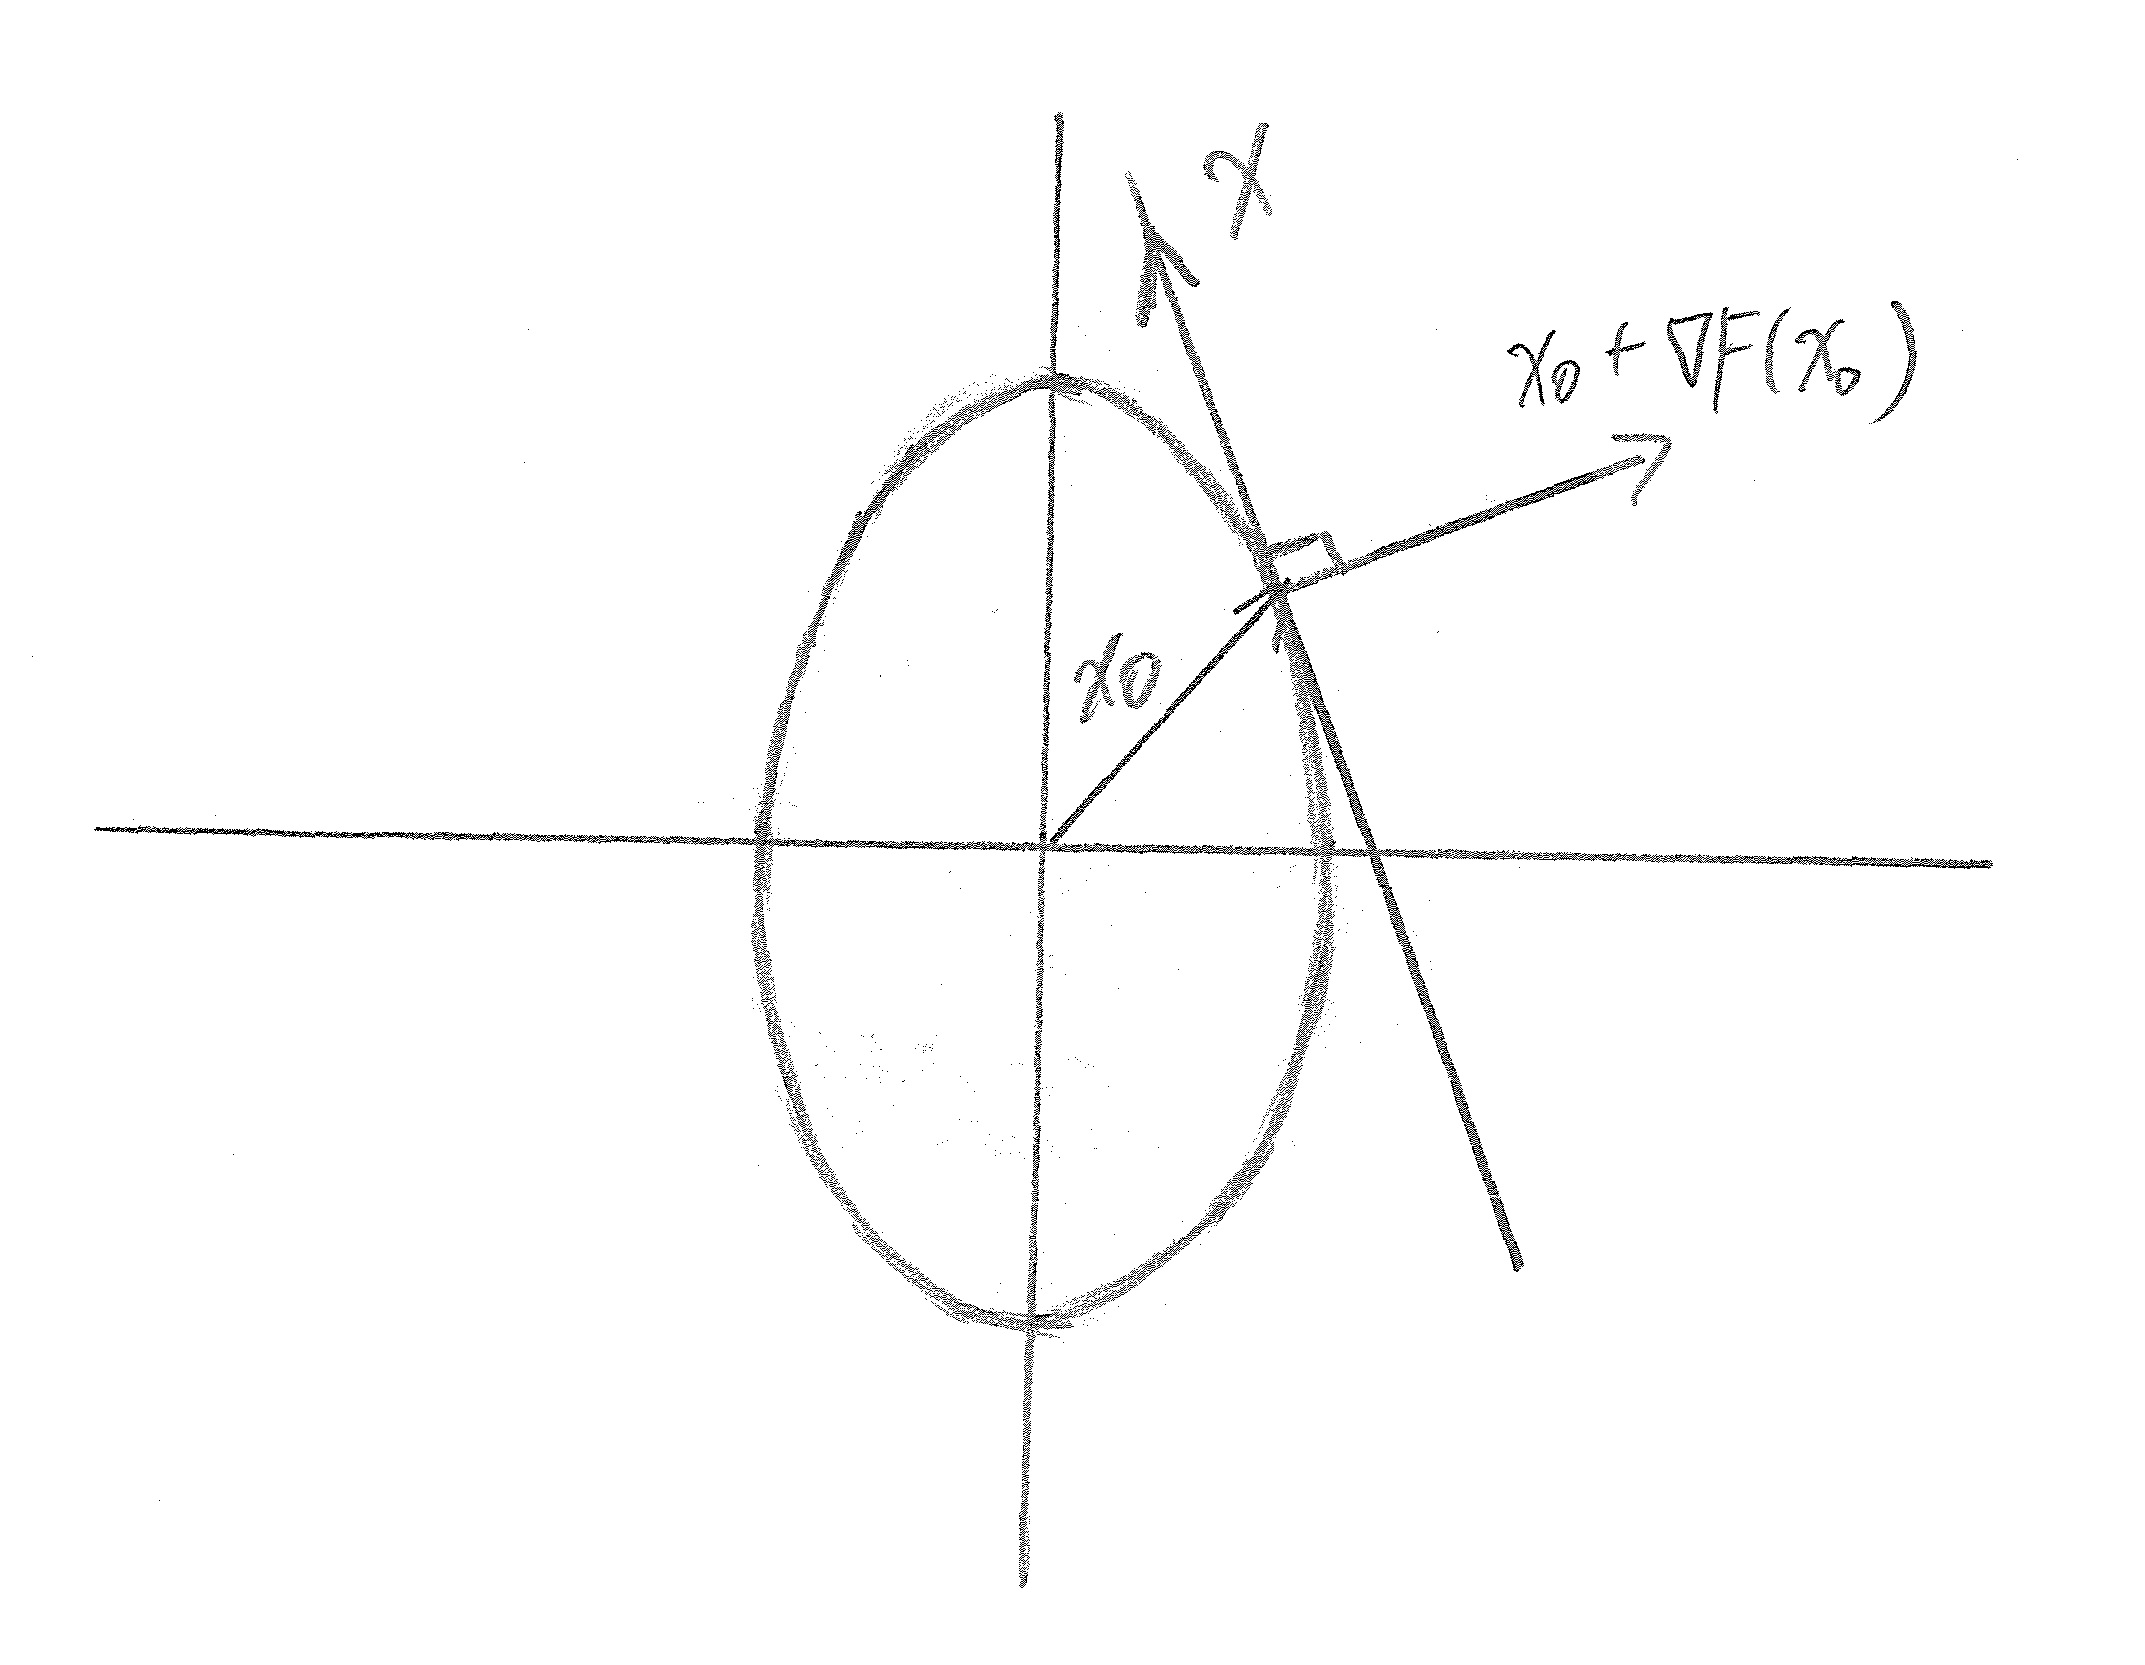
\includegraphics[width=2.1in,height=2.1in]{figures/ch02/p60-2.jpg}
	%\caption{This is an inserted JPG graphic} 
	%\label{fig:graph} 
\end{figure}


(2) Consider $c = \varepsilon > 0$, a small positive increment. Then, 
$$\{x | \nabla F(x_0)^{T} (x-x_0) = \varepsilon\}$$
is points that, to first order, have slightly higher cost (value, level). Then $F(x_0)$, the value at $x=x_0$.

\begin{figure}
	\centering
	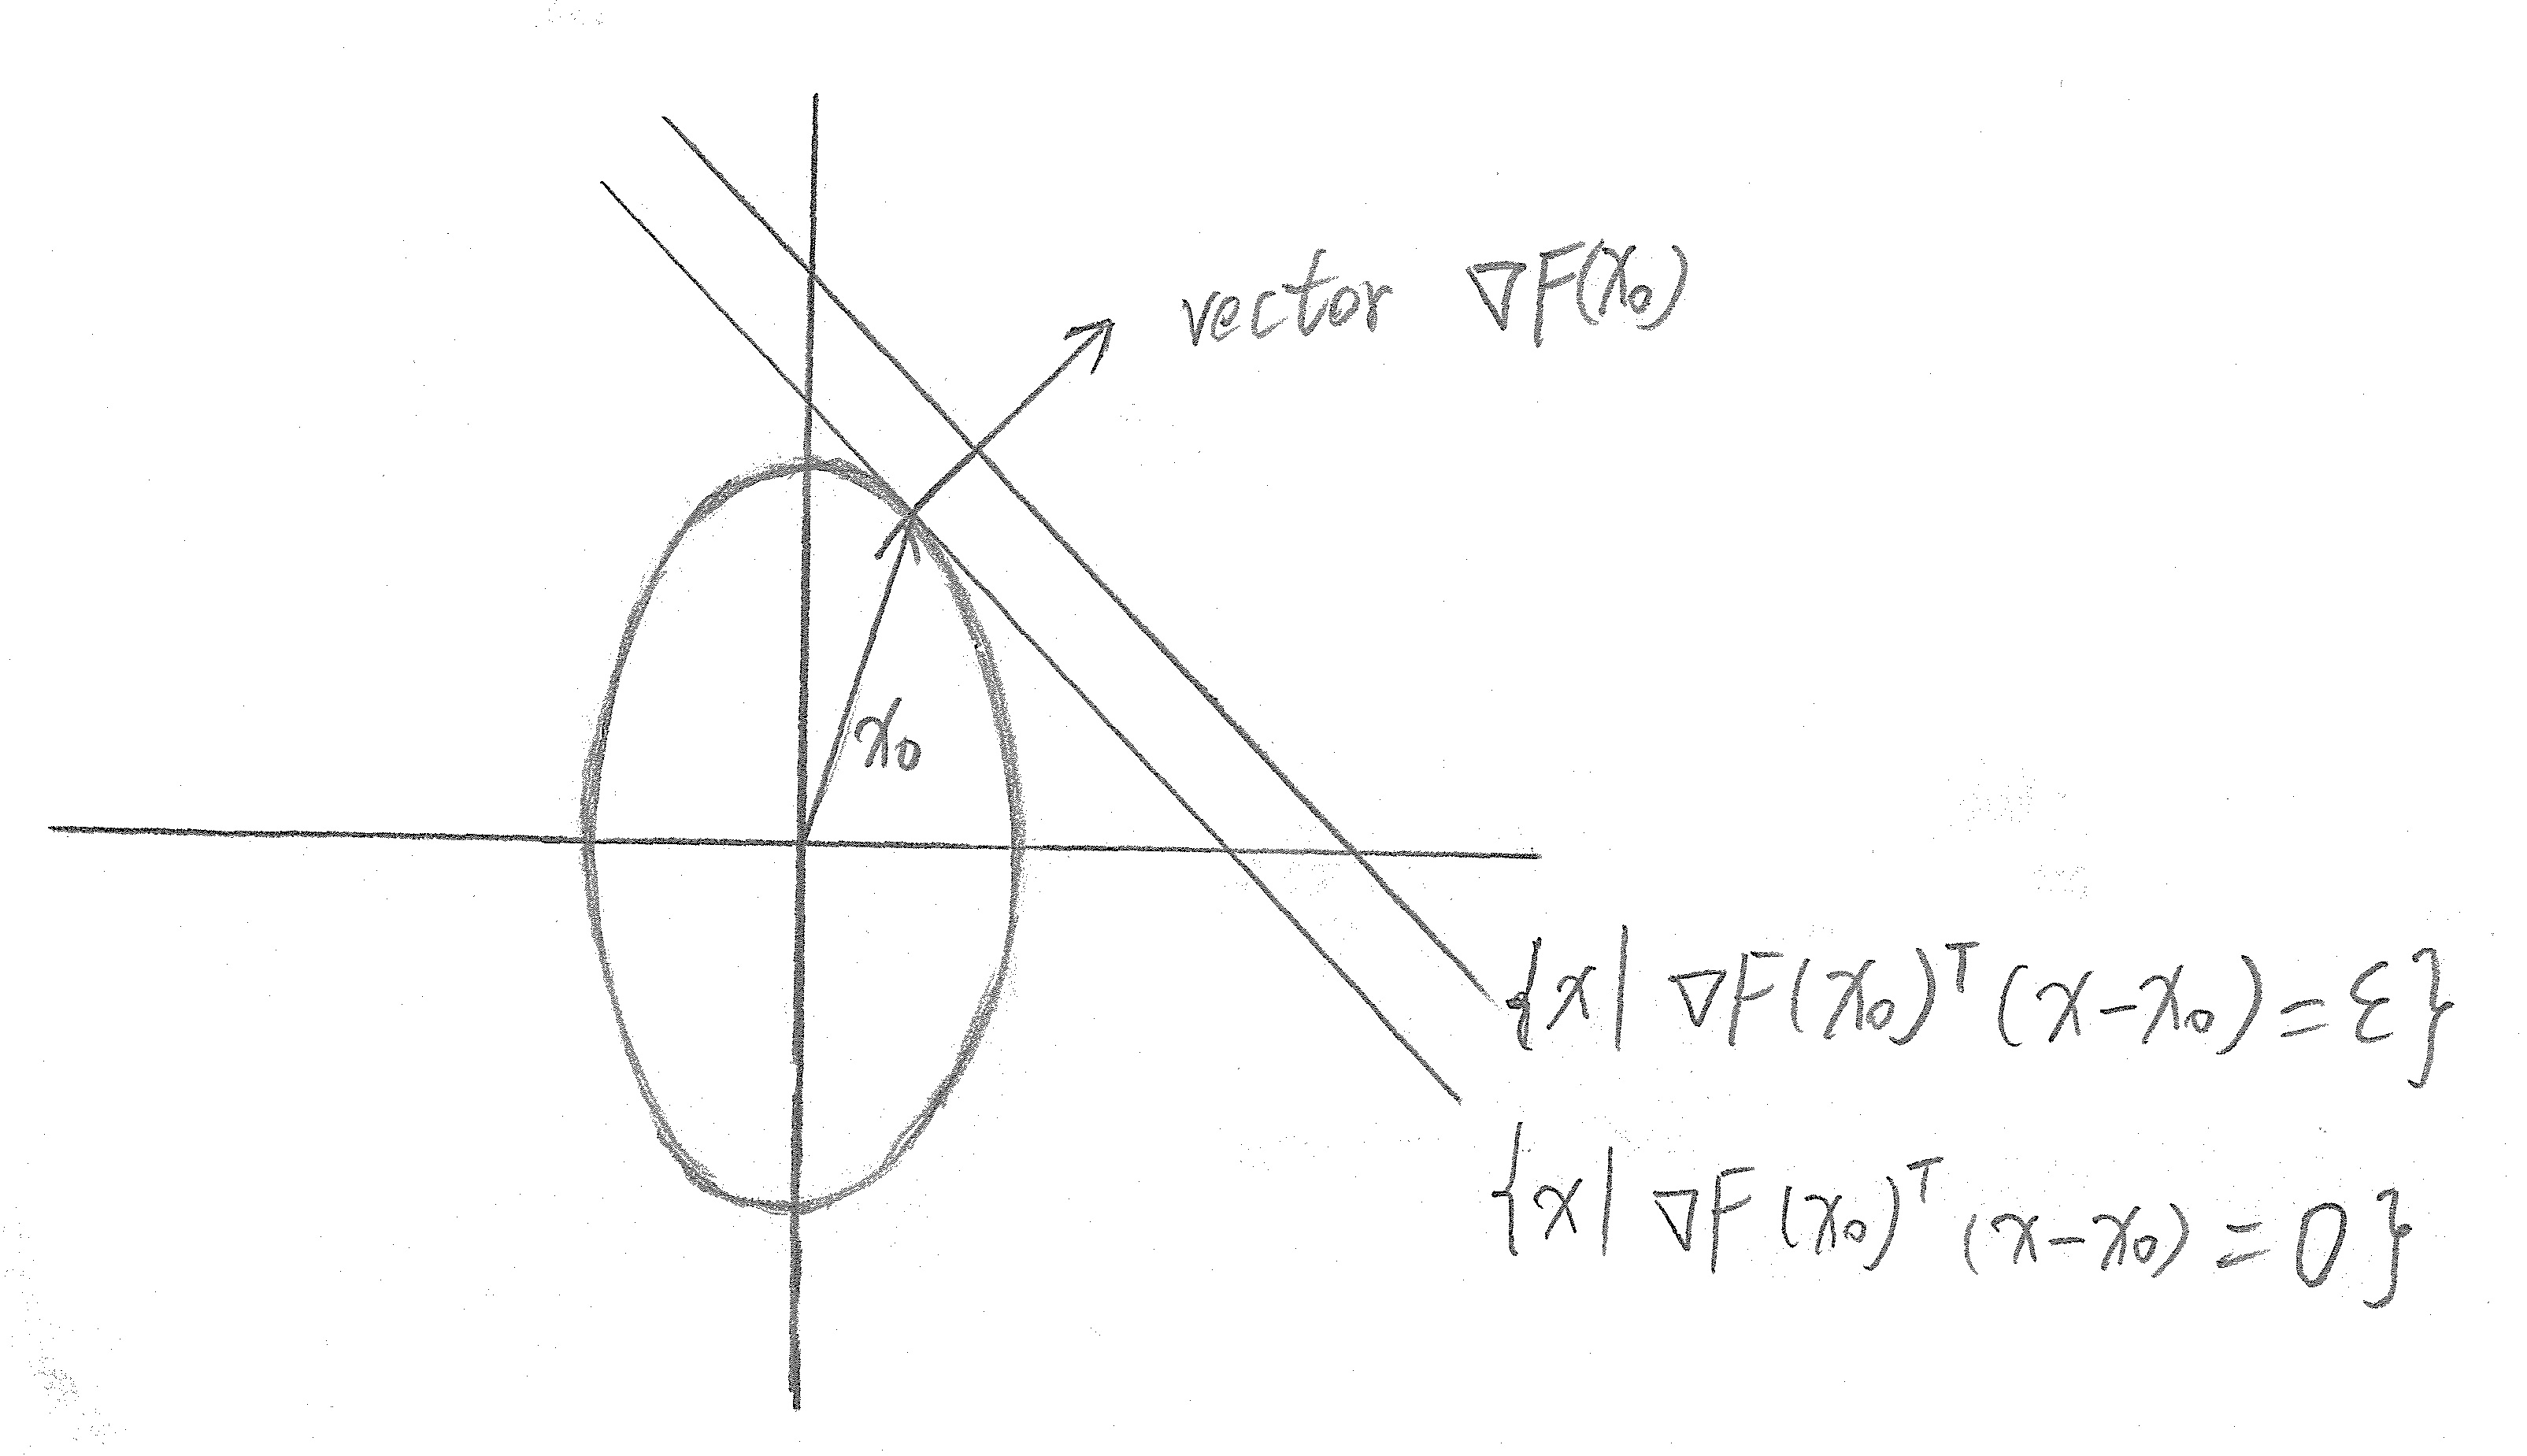
\includegraphics[width=2.1in,height=2.1in]{figures/ch02/p61.jpg}
	%\caption{This is an inserted JPG graphic} 
	%\label{fig:graph} 
\end{figure}

In general the set
\begin{align*}
&\{x | \nabla F(x_0)^{T} (x-x_0) = c\}\\
&= \{x | \nabla F(x_0)^{T} x = \nabla F(x_0)^{T} x_0 + c\} \\
&= \{x | a^{T}x = b\}
\end{align*}
which is a "hyperplane", a type of affine set. 

\vspace{0.5cm}
Observe that geometry of gradients connects to geometry of level sets. But you might think that is a bit funny. You know a Taylor sense approx is of the function $F$ not the level sets of $F$. You might also recall there is a tangent approximation involved somewhere, e.g. 

\begin{figure}
	\centering
	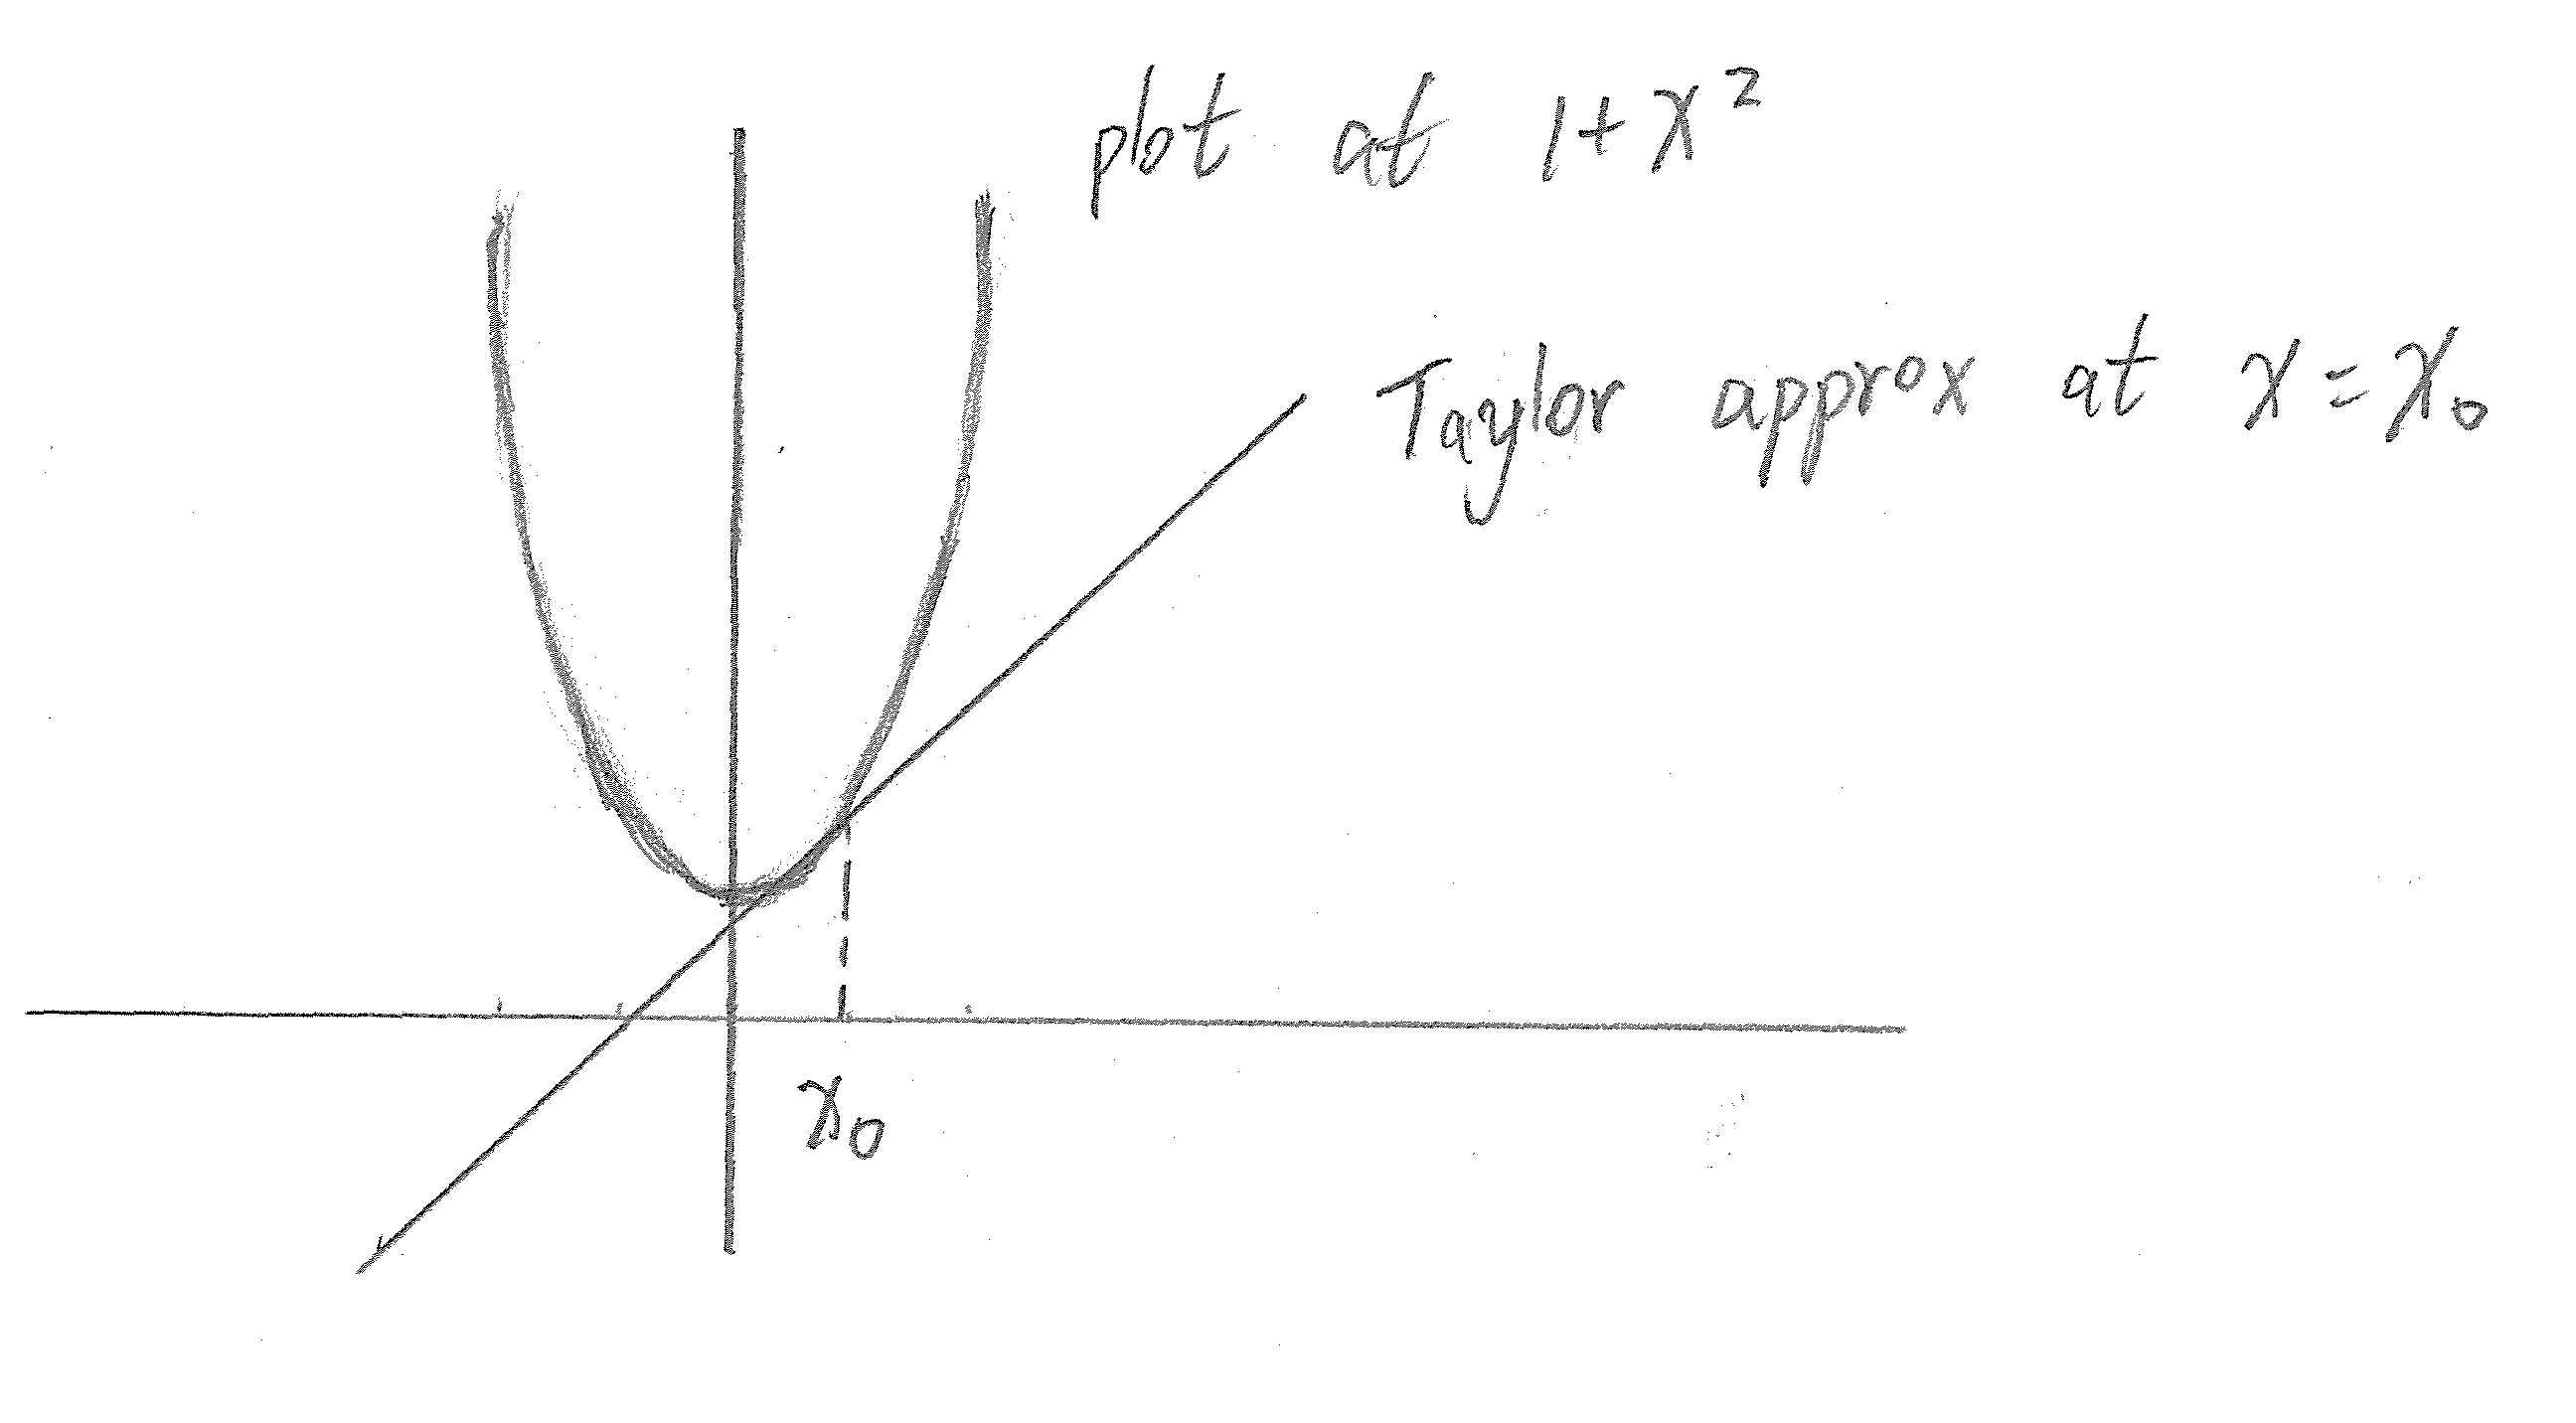
\includegraphics[width=2.1in,height=2.1in]{figures/ch02/p62.jpg}
	%\caption{This is an inserted JPG graphic} 
	%\label{fig:graph} 
\end{figure}


To develop the approximation we need to consider the plot or "graph" at the function $F$
$$\text{graph}\ F = \{(x, F(x) | x \in \mathbb{R}^n)\} \subseteq \mathbb{R}^{n+1}$$

e.g., in above example $F(x) = x^2+1$, $F \colon \mathbb{R} \to \mathbb{R}$, $s-n=1$ and plot (graph) is in $\mathbb{R}^2$.

To find the tangent approximation, we will pick a point $t$ "above". The graph, is pick some pair $(x, t)$ s.t. $t \geq F(x)$.

Use Taylor approximation above $x_0$ to approximate $F(x)$ 

\begin{figure}
	\centering
	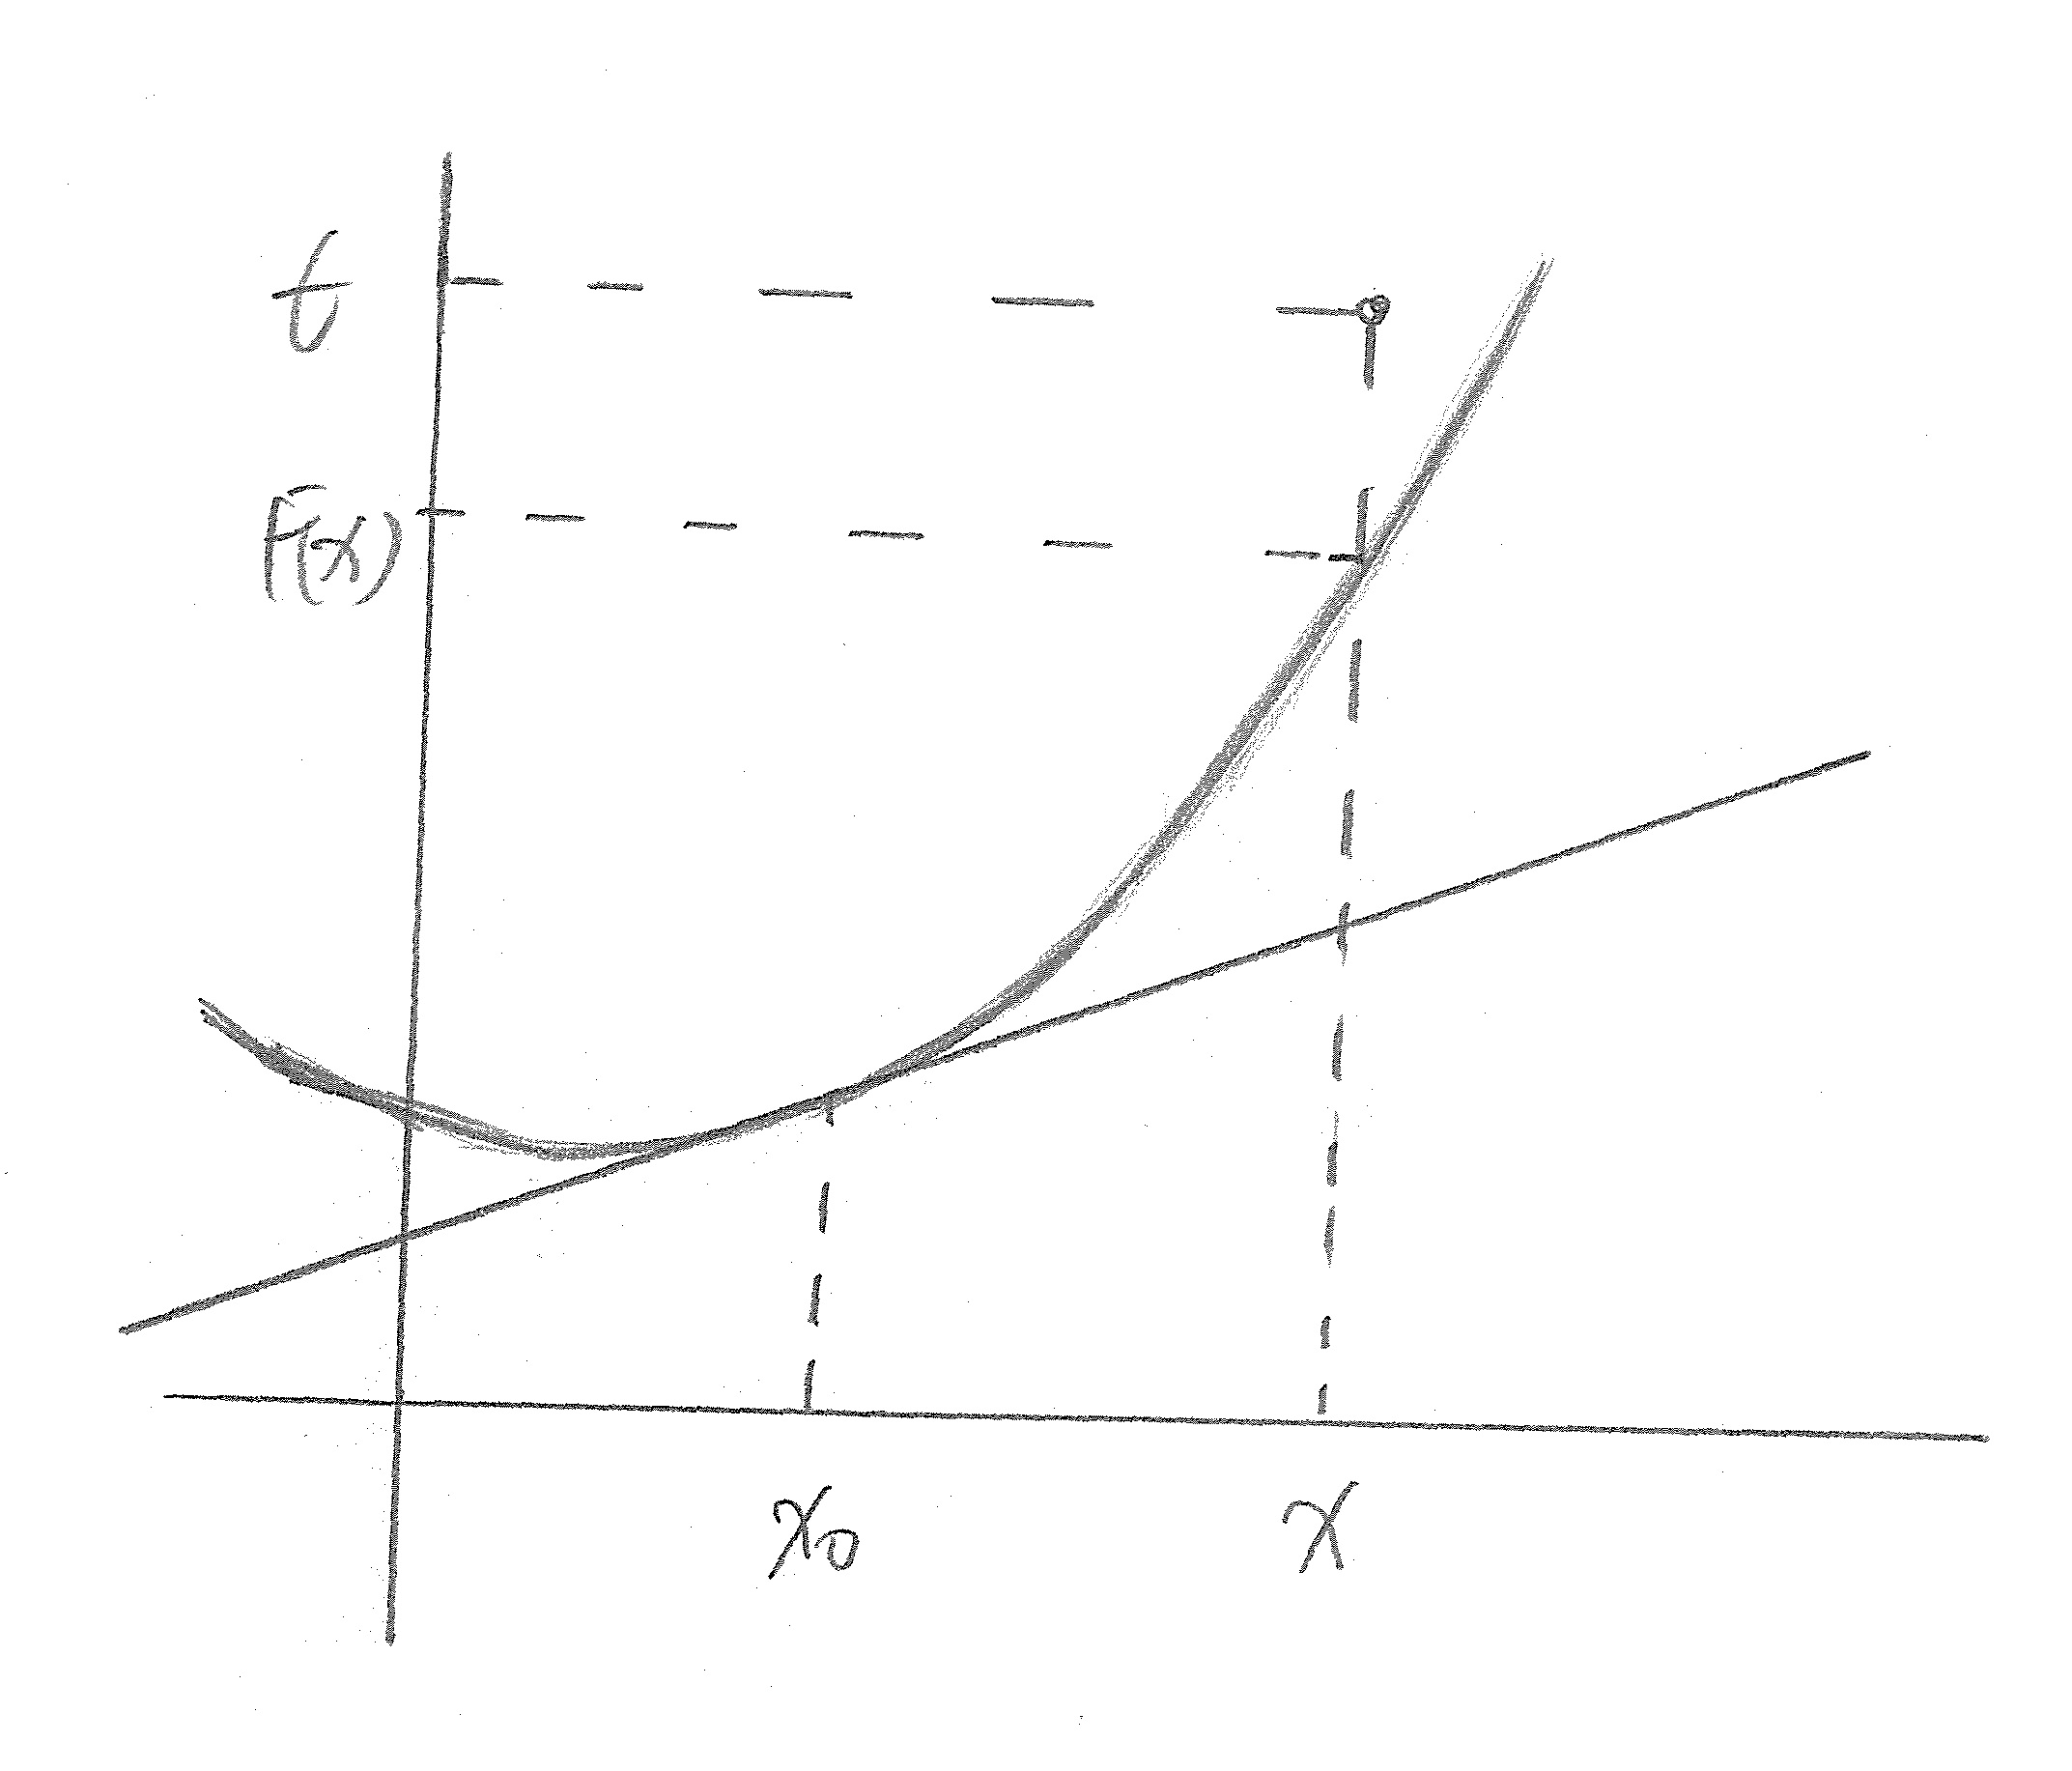
\includegraphics[width=2.1in,height=2.1in]{figures/ch02/p63.jpg}
	%\caption{This is an inserted JPG graphic} 
	%\label{fig:graph} 
\end{figure}

\vspace{0.5cm}
Recap:

(1) Pick $(x, t)$ s.t. $t \geq F(x)$
 
(2) Assume $x$ and $x_0$ are "close" so approximation is accurate.

(3) By Taylor
$F(x) = F(x_0) + \nabla F(x_0)^{T} (x-x_0) + \varepsilon(x)$

(4) By (1), $t \geq F(x) = F(x_0) + \nabla F(x_0)^{T} (x-x_0) + \varepsilon(x)$

(5) By (2) will drop the $\varepsilon(x)$ term and assume inequality doesn't flip (because $x$ and $x_0$ are sufficiently close that $\varepsilon(x)$ is sufficient small), and thus yields 
$$t \geq F(x_0) + \nabla F(x_0)^{T} (x-x_0)\qquad  (*)$$
Next, we re-arrange

(6)
\begin{align*}
0 &\geq -(t-F(x_0)) + \nabla F(x_0)^{T} (x - x_0) \\
&=\begin{bmatrix} \nabla F(x_0)^{T} -1\\ \end{bmatrix}  \begin{bmatrix} x-x_0\\ t-F(x_0)\\ \end{bmatrix} 
\end{align*}


Observe that:

(a) $(x-x_{0})\in \reals^{n}$ so vectors are in $\reals^{n+1}$.

(b) $t-F(x_{0})\in\reals$ i.e., in example plot when $n=1$ in $\reals^{2}$.

\begin{figure}
	\centering
	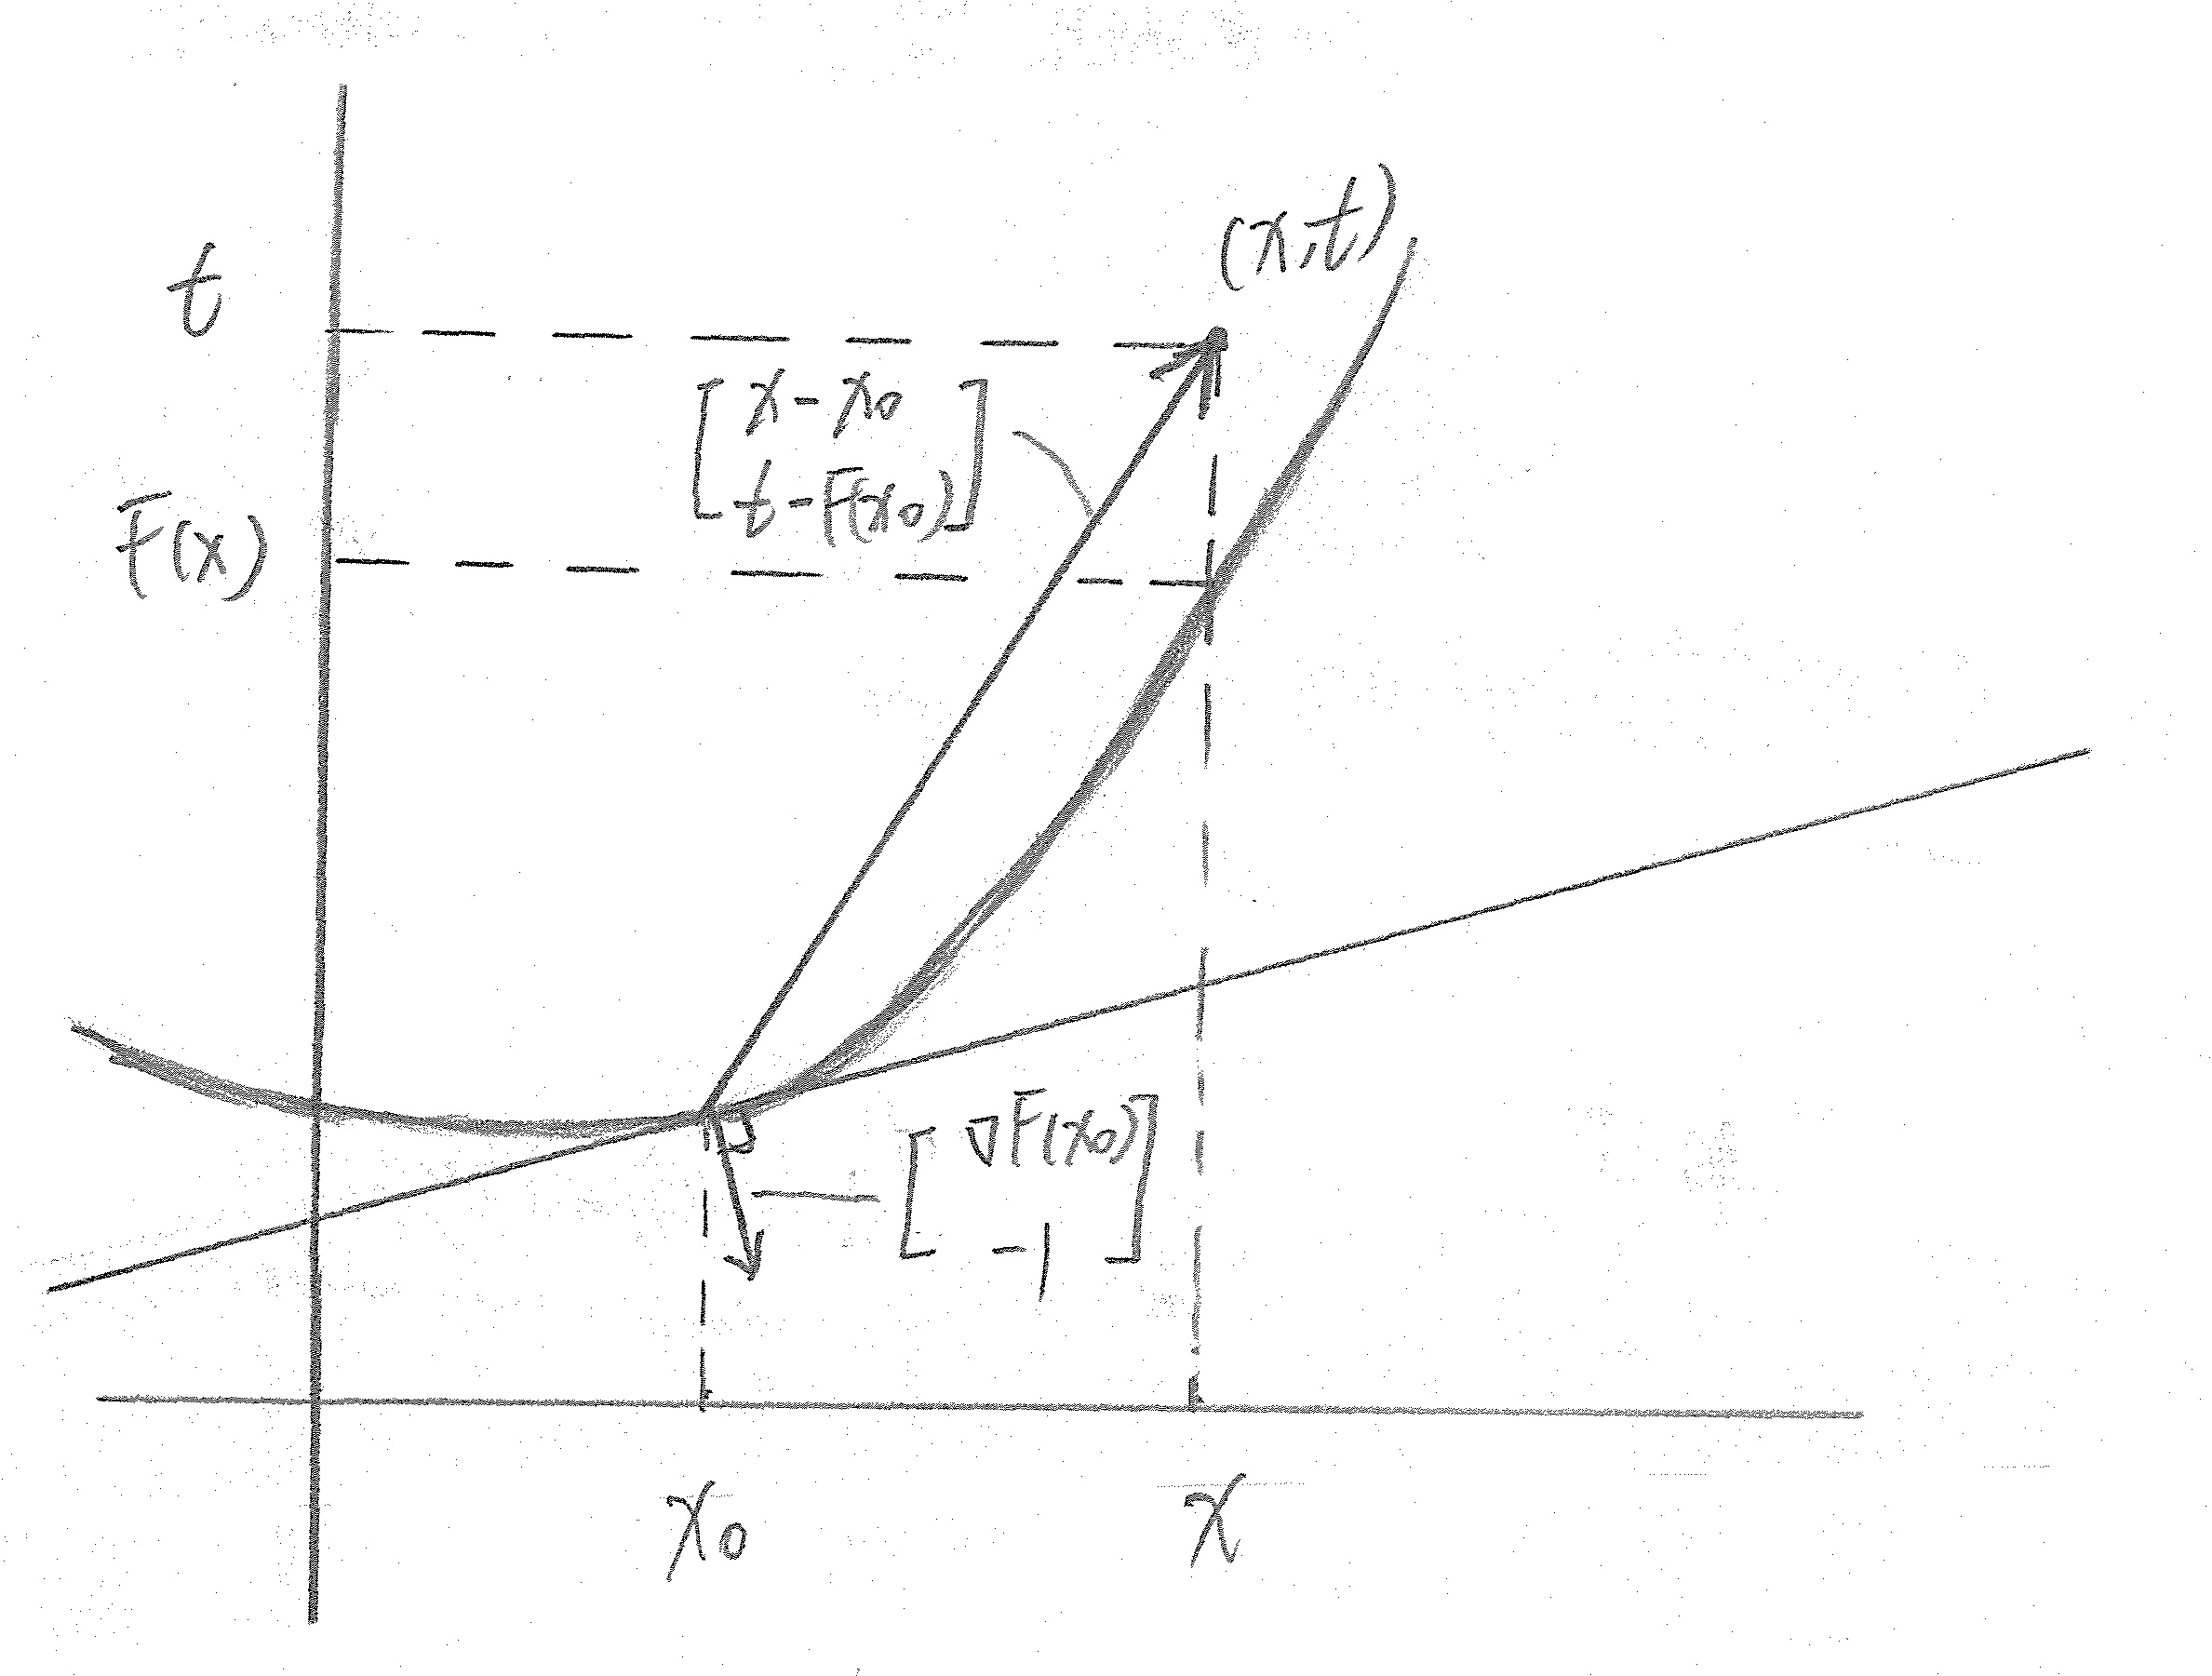
\includegraphics[width=2.1in,height=2.1in]{figures/ch02/p64.jpg}
	%\caption{This is an inserted JPG graphic} 
	%\label{fig:graph} 
\end{figure}

\vspace{0.5cm}
Now recall connection between angles and inner products.

(1). If inner product of 2 vectors is negative, then the angles is obtuse.

(2). Matches picture.

What about vectors when this inner product = 0 ? That is
$$\{u\in\reals^{n+1}|\langle u, [\nabla F(x_{0}) , -1]^{\trans}\rangle=0\}$$

writing $u=[x-x_{0}, t-F(x_{0}]^{\trans}$ and no longer require $t\geq F(x)$.

The condition becomes
$$
\left[
\begin{array}{c} 
	x-x_{0}\\
	t-F(x_{0})
\end{array}
\right]^{\trans}  
\left[
\begin{array}{c} 
\nabla F(x_{0})\\
-1
\end{array}
\right]
=
0
$$

So we recognize the set defines a hyperplane in $\reals^{n+1}$,
$$\mathcal{H}=\left\{\left[
\begin{array}{c} 
	x \\
    t
\end{array}
\right]  
\middle|      
\left[
\begin{array}{cc} 
x^{\trans}&t
\end{array}
\right]  
\left[
\begin{array}{c} 
\nabla F(x_{0}) \\
-1
\end{array}
\right]  
=
\left[
\begin{array}{cc} 
x_{0}^{\trans}&F(x_{0})
\end{array}
\right]  
\left[
\begin{array}{c} 
	\nabla F(x_{0}) \\
	-1
\end{array}
\right]  
\right\}$$
This is called a "supporting hyperplane" of the epigraph.

Finally, let's look at Taylor approximation one last time (1st order approximation), and recall the geometric interpretation of each of the pieces:
\begin{align*}
F(x)&\approx F(x_{0})+ \nabla F(x_{0})^{\trans}(x-x_{0})\\
&=F(x_{0})+\Vert\nabla F(x_{0})\Vert \Vert x-x_{0}\Vert \left< \frac{\nabla F(x_{0})}{\Vert\nabla F(x_{0})\Vert},\frac{x-x_{0}}{\Vert x-x_{0}\Vert}\right>\\
&=\text{bias + steepness $\times$ distance $\times$ angle }
\end{align*}
























 












\chapter{Matrices and eigen decomposition}
\label{ch.matEig}
\section{Matrices: array of numbers}

%Lecture 9.11




Matrices are rectangular arrays of numbers:

$$
A = 
\left[
\begin{matrix}
a_{11} & a_{12} & ... & a_{1n} \\
a_{21} & a_{22} & ... & a_{2n} \\
... & ... & ... & ...\\
a_{m1} & a_{m2} & ... & a_{mn}
\end{matrix}
\right] \in \Re^{m\times n}
$$


The element in the $i^{th}$ row \& $j^{th}$ column: $a_{ij} = [A]_{ij}$(equivalent notation)

The transposition operation works on matrices by exchanging rows and columns: 

$$
A^T = 
\left[
\begin{matrix}
a_{11} & a_{21} & ... & a_{1n} \\
a_{12} & a_{22} & ... & a_{m2} \\
... & ... & ... & ...\\
a_{1n} & a_{2n} & ... & a_{mn}
\end{matrix}
\right] \in \Re^{m\times n}
$$

So $[A]_{ij}  = [A^T]_{ji}$ if $A\in \Re^{m\times n}$ and $A^T\in \Re^{n\times m}$


1) $A + B = C$ where $[C] = [A]_{ij} + [B]_{ij}$

2) $\alpha A = B$ where $[B]l_{ij} = \alpha [A]_{ij}$

The origin is a all-zero matrix. 

\begin{definition}{Inner Product}
	$<A, B> = trace(A^TB) = trace(BA^T)$ where $A^TB\in \Re^{n\times n}$ and $B^TA\in \Re^{m\times m}$
\end{definition}

where trace(X) is defined as the sum of the diagonal elements of X. \\

Forbenius Norm: $||A||_F = \sqrt{<A, A>} = \sqrt{trace(A^TA)} = \sqrt{\sum^m_{i=1}\sum^m_{j=1}[A]^2_{ij}}$


$$\vec{(A)} = \text{vec}
\left(
\left[
\begin{matrix}
... & ... & ... & ... \\
a_{1} & a_{2} & ... & a_{n} \\
... & ... & ... & ...
\end{matrix}
\right]\right) = 
\left[
\begin{matrix}
a_{1} \\
a_{2} \\
... \\
a_{n}
\end{matrix}
\right]
\in \Re^{m\times n}
$$

Matrix inverse: if $A$ is "invertible", $\exists$ unique $A^{-1}$ s.t. $AA^{-1} = A^{-1}A = I$

\begin{itemize}
	\item $(AB)^{-1} = B^{-1}A^{-1}$
	
	\item $(A^{-1})^T = (A^T)^{-1}$
	
	\item $det(A^{-1}) = \frac{1}{det(A)}$
\end{itemize}

\subsection{Matrices as linear \& affine maps}


$x\in \Re^n \rightarrow A \rightarrow y = Ax \in \Re^m$\\

Affine maps are linear functions plus a constant term: $y = Ax + b$ where $A\in \Re^{m,n}$, $b\in \Re^m$

\subsection{Approximations}

A nonlinear map $f: \Re^n \rightarrow \Re^m$ can be approximated by an affine map:

\begin{equation*}
f(x) = f(x_0) + J_f(x_0)(x - x_0) + o(||x - x_0||)
\end{equation*}

where $o(||x - x_0||)$ are terms go to 0 faster than 1st order for $x\rightarrow x_0$ and $J_f(x_0)$ is the Jacobian of $f$ at $x_0$:




$$J_f(x_0) = 
\left[
\begin{matrix}
\frac{\sigma f_1}{\sigma x_1} &  ... & \frac{\sigma f_1}{\sigma x_n} \\
... &  ... & ...\\
\frac{\sigma f_m}{\sigma x_1} &  ... &\frac{\sigma f_m}{\sigma x_n}
\end{matrix}
\right]_{x = x_0}
$$

For $x$ 'near' $x_0$, the variation $\delta_f(x) =f(x) - f(x_0)$ can be approximated described by a linear map:

\begin{equation*}
\delta_f(x) = J_f(x_0)\delta_x, \,\, \delta_x = x - x_0
\end{equation*}
\subsection{Orthogonal Matrices}

\begin{definition}
	$U\in \Re^{n\times m}$ is \textbf{orthogonal} if $U = [U^{(1)} ... U^{(n)}]$
	and 
	
	$$ U^{(1)^T}U^{(1)}=\left\{
	\begin{aligned}
	0\,\, \forall i\neq j \\
	1\,\, if \,\, i = j
	\end{aligned}
	\right.
	$$
\end{definition}

Then $UU^T = U^TU = I$\\


$x\rightarrow U \rightarrow y = Ux$

\begin{equation*}
||y||^2 = (Ux)^T(Ux) = x^TU^TUx = x^Tx = ||x||^2
\end{equation*}

$<Ux, Uw> = x^TU^TUw = x^Tw = <x, w>$

\begin{itemize}
	\item Domain
\end{itemize}

$dom(A)$ = $\Re^n$, $A = [a^{(1)}...a^{(n)}]$

$dom(A^T)$ = $\Re^m$, $A^T = [a^{(1)}...a^{(m)}]$


\begin{itemize}
	\item Range
\end{itemize}

Range of A is the set of vectors $y$ obtained as a linear combination of the $a_i$s are of the form $y= Ax$ for some vector $x\in \Re^n$.

\begin{equation*}
R(A) = \{y\in \Re^m | y = Ax = \sum^n_{i=1}x_ia^{(i)}\}
\end{equation*}

\begin{equation*}
R(A^T) = \{w\in \Re^m | w = A^Tu = \sum^m_{i=1}u_ia^{(i)}\}
\end{equation*}

\begin{itemize}
	\item Rank
\end{itemize}

The dimension of $R(A)$ is called the rank of $A$:

\begin{equation*}
rank(A) = dim\{R(A)\} = dim\{R(A^T)\} = rank(A^T)
\end{equation*}

\begin{itemize}
	\item Nullspace
\end{itemize}

The nullspace of the matrix $A$ is he set of vectors in the input space that are mapped to zero:

\begin{equation*}
N(A) = \{x\in \Re^n | Ax = 0\}
\end{equation*}

\begin{itemize}
	\item Fundamental Theorem
\end{itemize}

We can find that for any $x\in \Re(A^T)$ and any $z\in \mathcal{N}(A)$, it holds that $x^Tz = 0$.\\

$\Re^n = \Re(A^T) \bigoplus N(A)$: $\forall x\in \Re^n$ there is a unique $x = x_{R(A^T)} = x_{N(A)}$.\\

\begin{theorem}{Fundamental theorem of linear algebra}
	For any given matrix $A\in \Re^{m,n}$, it holds that $\mathcal{N}(A) \perp \mathcal{R}(A^T)$ and $\mathcal{R}(A) \perp \mathcal{N}(A^T)$, hence
	
	\begin{align*}
	\mathcal{N}(A) \bigoplus \mathcal{R}(A^T) &= \Re^n\\
	\mathcal{R}(A) \bigoplus \mathcal{N}(A^T) &= \Re^m\\
	dim \mathcal{N}(A) + rank(A) &=n\\
	dim \mathcal{N}(A^T) + rank(A) &=m
	\end{align*}
\end{theorem}

Consequently we can decompose $\forall x\in \Re^n$ as the sum of 2 vectors orthogonal to each other, one in range of $A^T$ and another in nullspace of $A$:

\begin{equation*}
x = A^T\xi + z, z\in \mathcal{N}(A)
\end{equation*}




\subsection{PageRank}

%Lecture Sep 16

For the PageRank algorithm, more important webpages should be ranked higher:


Let us assume each node’s importance score is evenly spread across all the outgoing links, each node’s importance score can also be written as the sum of the importance scores received from all of the incoming neighbors: for node A, $\sum_{j \rightarrow A}\frac{\pi_j}{O_j}$


\begin{figure}
	\centering
	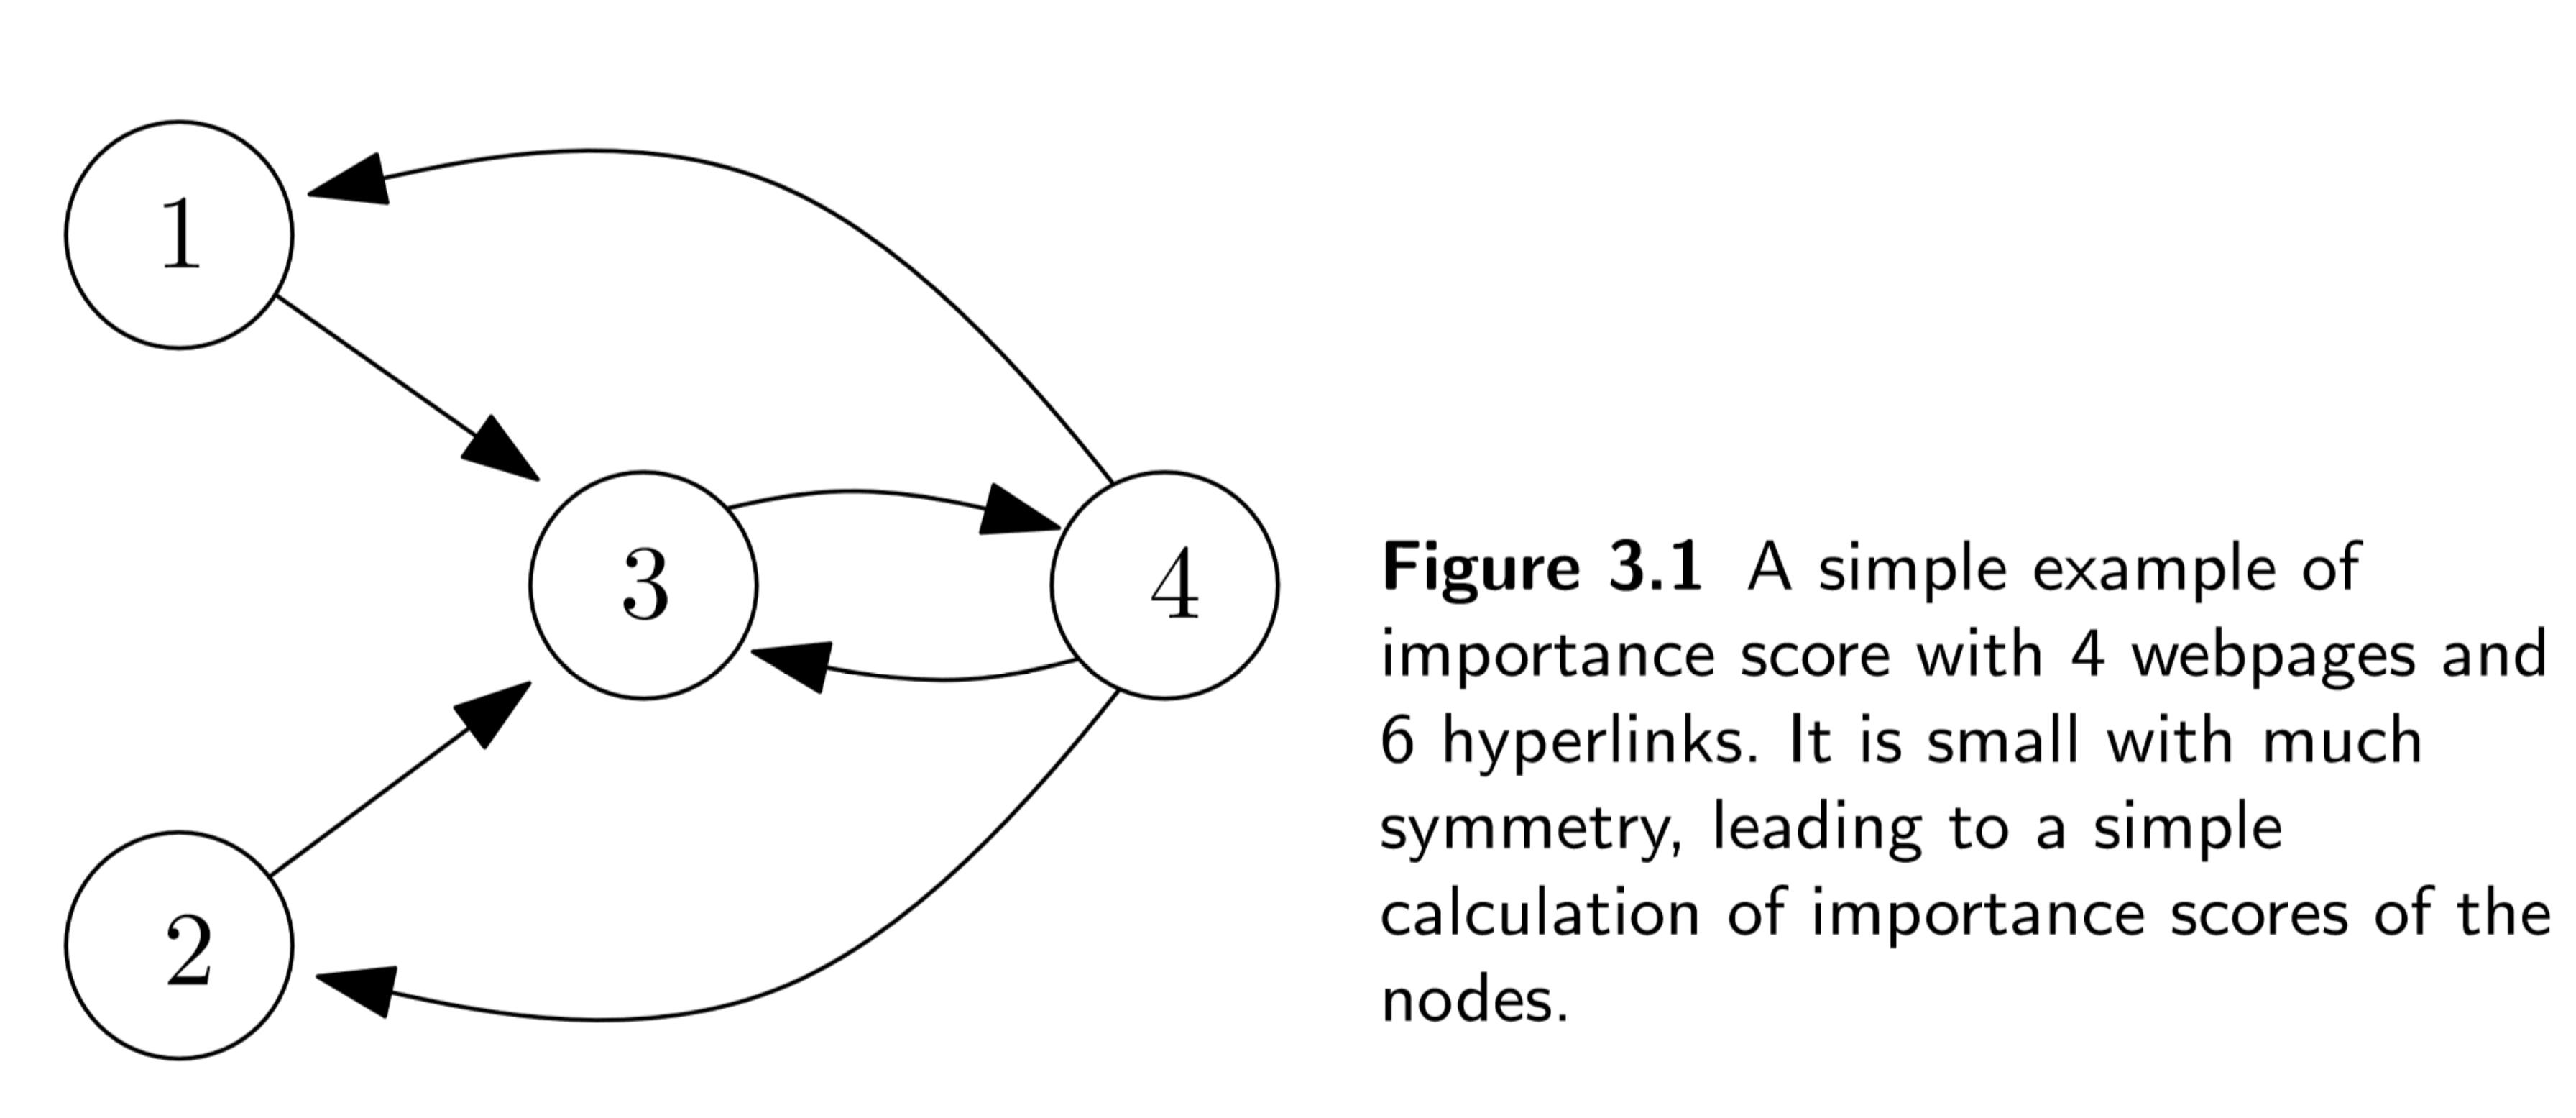
\includegraphics[width=2.1in,height=2.1in]{figures/ch03/figure0.jpg}
	%\caption{This is an inserted JPG graphic} 
	%\label{fig:graph} 
\end{figure}


Let the score of node 1 (and 2) be x, and that of node 3 (and 4) be y. Looking at node 1's incoming links, we see that there is only one such link, coming from node 4 that points to three nodes. So $x = \frac{y}{3}$ and $2x + 2y = 1$, so set of importance scores turns out to be [0.125, 0.125, 0.375, 0.375].

Matrix $H$: its $(i,j)$th entry is $\frac{1}{O_i}$ if there is a hyperlink from webpage i to webpage j, and 0 otherwise.

$\pi$: $N \times$1 column vector denoting the importance scores of the N webpages.

Multiply $\pi^T$ on the right by matrix $H$, this is spreading the importance score from the last iteration evenly among the outgoing links, and re-calculating the importance score of each webpage in this iteration by summing up the importance scores from the incoming links.

Note: $\pi^T[k] = \pi^T[k - 1]H$



Note: $\pi^T[k] = \pi^T[k - 1]G$

Obviously, $\pi^{T}$ is the left eigenvector of $G$ corresponding to the eigenvalue of 1: $\pi^{T} = \pi^{*T}G$.

For a graph like this:

\begin{figure}
	\centering
	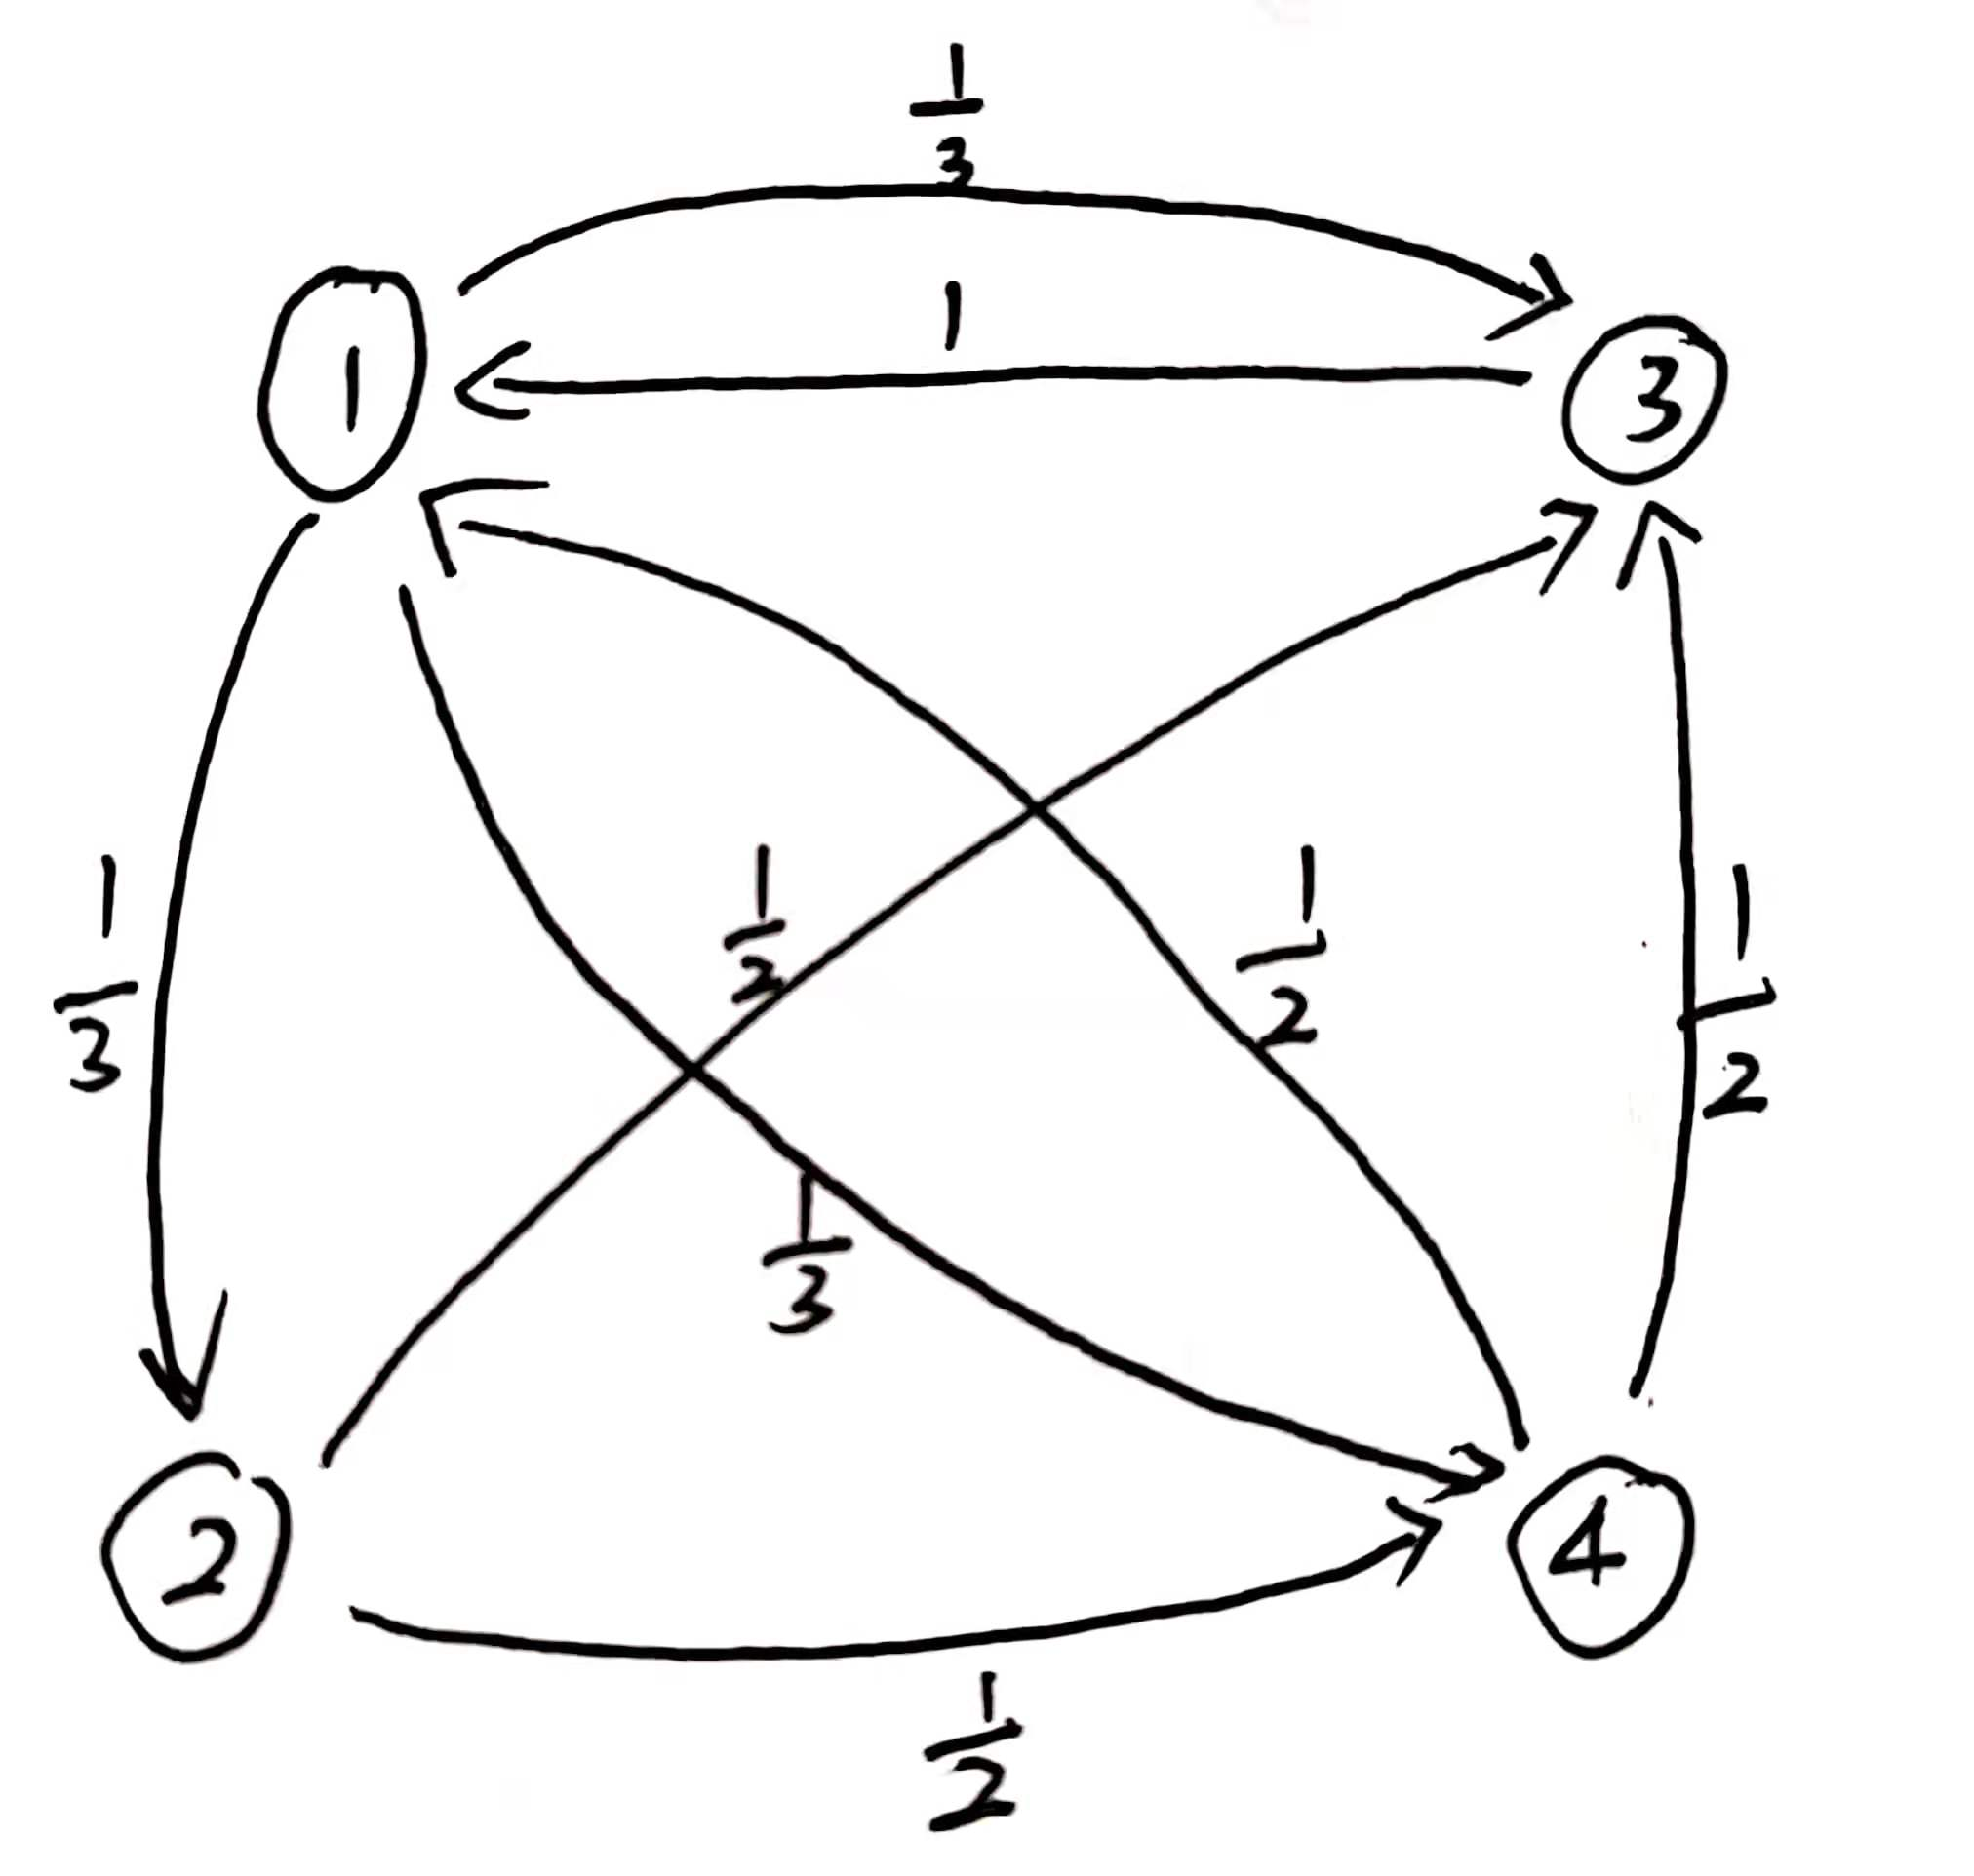
\includegraphics[width=2.1in,height=2.1in]{figures/ch03/figure3.jpg}
	%\caption{This is an inserted JPG graphic} 
	%\label{fig:graph} 
\end{figure}



$$
\left[
\begin{matrix}
x_1 \\
x_2 \\
x_3\\
x_4\\
\end{matrix}
\right] =
\left[
\begin{matrix}
0 & 0 & 1 & \frac{1}{2} \\
\frac{1}{3} & 0 & 0& 0 \\
\frac{1}{3}& \frac{1}{2} & 0 & \frac{1}{2} \\
\frac{1}{3} & \frac{1}{2} & 0 & 0 
\end{matrix}
\right]
\left[
\begin{matrix}
x_1 \\
x_2 \\
x_3\\
x_4\\
\end{matrix}
\right]
$$

\begin{align*}
x &= Ax \\
Ax - x &= 0\\
(A - I)x &= 0\\
x&\in N(A-I)
\end{align*}


$$
x = \frac{1}{s_1}
\left[
\begin{matrix}
12 \\
4 \\
9\\
6\\
\end{matrix}
\right]
$$
Note: 

\begin{itemize}
	\item $x^{(0)}$ is the initial distribution.
	
	\item $x^{(0)}_i = $Pr[start on page $i$]
	
	\item $u^{(i)}, \lambda_i$ is eigen-vector/value pair if $Au^{(i)} = \lambda_iu^{(i)}$
\end{itemize}


If $Au^{(i)} = \lambda_iu^{(i)}$, $A$ is "diagonalizable" if it has a full set of linear independent eigenvectors. In this case $x^{(0)} = \sum^n_{i=1}\alpha_iu^{(i)}$

\begin{align*}
x^{(1)} &= Ax^{(0)} = A[\sum^n_{i=1}\alpha_iu^{(1)} = \sum_i\alpha_i(Au^{(i)})]\\
x^{(2)} &= A(Ax^{(0)}) = \sum^n_{i=1}\alpha_i(A^2u^{(i)}) = \sum^n_{i=1}\alpha_i(\lambda_i^2u^{(i)})\\
...\\
x^{(k)} &= A^kx{(0)} = \sum^n_{i=1}\alpha_i(\lambda_i)^ku^{(i)}\\
&= \alpha_1(\lambda_1)^ku^{(1)} + \sum^n_{i=2}\alpha_i(\lambda_i)^ku^{(i)} \\
&= \alpha_1u^{(1)} + \sum^n_{i=2}\alpha_i(\lambda_i)^ku^{(i)}\\
&when \,k \rightarrow \infty\\
&= \alpha_1u^{(1)}
\end{align*}

\begin{equation*}
lim_{k\rightarrow \infty}\frac{A^kx^{(0)}}{||A^kx^{(0)}||} =u^{(i)}
\end{equation*}

%What is an Internet Structure s.t. $dim[N(A-I)] = 2$?

If have repeated eigenvalues:

\begin{align*}
Au^{(1)} =\lambda_1u^{(1)}\\
Au^{(2)} =\lambda_2u^{(2)}
\end{align*}

clearly:

\begin{equation*}
A(\alpha_1u^{(1)} + \alpha_2u^{(2)}) = \alpha_1\lambda_1u^{(1)} + \alpha_2\lambda_2u^{(2)}
\end{equation*}

where $\alpha_1u^{(1)} + \alpha_2u^{(2)}$ is this linear combination and $\alpha_1\lambda_1u^{(1)} + \alpha_2\lambda_2u^{(2)}$ are the maps to a different of same eigenvalues.

1) The "algebraic" multiplicity of an eignevalue $\lambda$ of a square matrix $A$ is \# of eigenvalues $\lambda_i, \lambda_2,...,\lambda_m$ equal to $\lambda$. $\rightarrow$ AM($\lambda$)

2) The geometric multiplicity of an eigenvalue $\lambda$ of a square matrix $A$ is the dimension of $N(A - \lambda I)$. $\rightarrow$ GM($\lambda$)

In general, $0 < GM(\lambda) \leq AM(\lambda)$ \& If $GM(\lambda_i) = AM(\lambda_i)$, $\forall i$, then $A$ is diagonalizable. 


If diagonalizable, we can write $Au^{(i)} = \lambda_iu^{(i)} \rightarrow$ assume all $\lambda_i$ distinct $GM(\lambda_i) = AM(\lambda_i) = 1, \forall i$

$$
\left[
\begin{matrix}
Au^{(1)} & Au^{(2)} &... &Au^{(n)} 
\end{matrix}
\right] =
\left[
\begin{matrix}
\lambda_1u^{(1)} & \lambda_2u^{(2)}&... &\lambda_iu^{(i)}
\end{matrix}
\right]
$$

$$A
\left[
\begin{matrix}
u^{(1)} & u^{(2)} &... &u^{(n)} 
\end{matrix}
\right] =
\left[
\begin{matrix}
u^{(1)} & u^{(2)} &... &u^{(n)}
\end{matrix}
\right]
\left[
\begin{matrix}
\lambda_1 & 0 & ... & 0\\
0& \lambda_2  &  ... & 0\\
...  & ...  &   ...& \\
0    &  ... &  0 & \lambda_n
\end{matrix}
\right]
$$



\begin{align*}
AU &= U\Lambda\\
A &= U\Lambda U^{-1}\\
\Lambda &= U^{-1}AU
\end{align*}

Recall pagerank:

\begin{align*}
A^kx^{(0)} &= (U\Lambda U^{-1})^kx^{(0)}\\
&=U\Lambda^kU^{-1}x^{(0)} \\
&= U
\begin{bmatrix}
\lambda_1^k & 0 & ... & 0\\
0& \lambda_2^k  &  ... & 0\\
...  & ...  &   ...& \\
0    &  ... &  0 & \lambda_n^k
\end{bmatrix} U^{-1}x^{(0)}
\end{align*}

\subsection{Determinant}

In eigen-decomposition, we need to solve for $\lambda$ from $det(A - \lambda I) = 0$. 
If $det(A) = 0$ then $A$ is non-invertible. 

Example:

$$A = 
\left[
\begin{matrix}
a_{11} & a_{12}\\
a_{21} & a_{22}
\end{matrix}
\right] =
\left[
\begin{matrix}
a_{(1)} & a_{(2)}
\end{matrix}
\right]
$$

\begin{align*}
U &= \{x\in \Re^2 | 0\leq x_1 \leq 1, 0\leq x_1 \leq 1 \}\\
P &= \{Ax, \ x\in \mathcal{U}\} 
\end{align*}

\begin{figure}
	\centering
	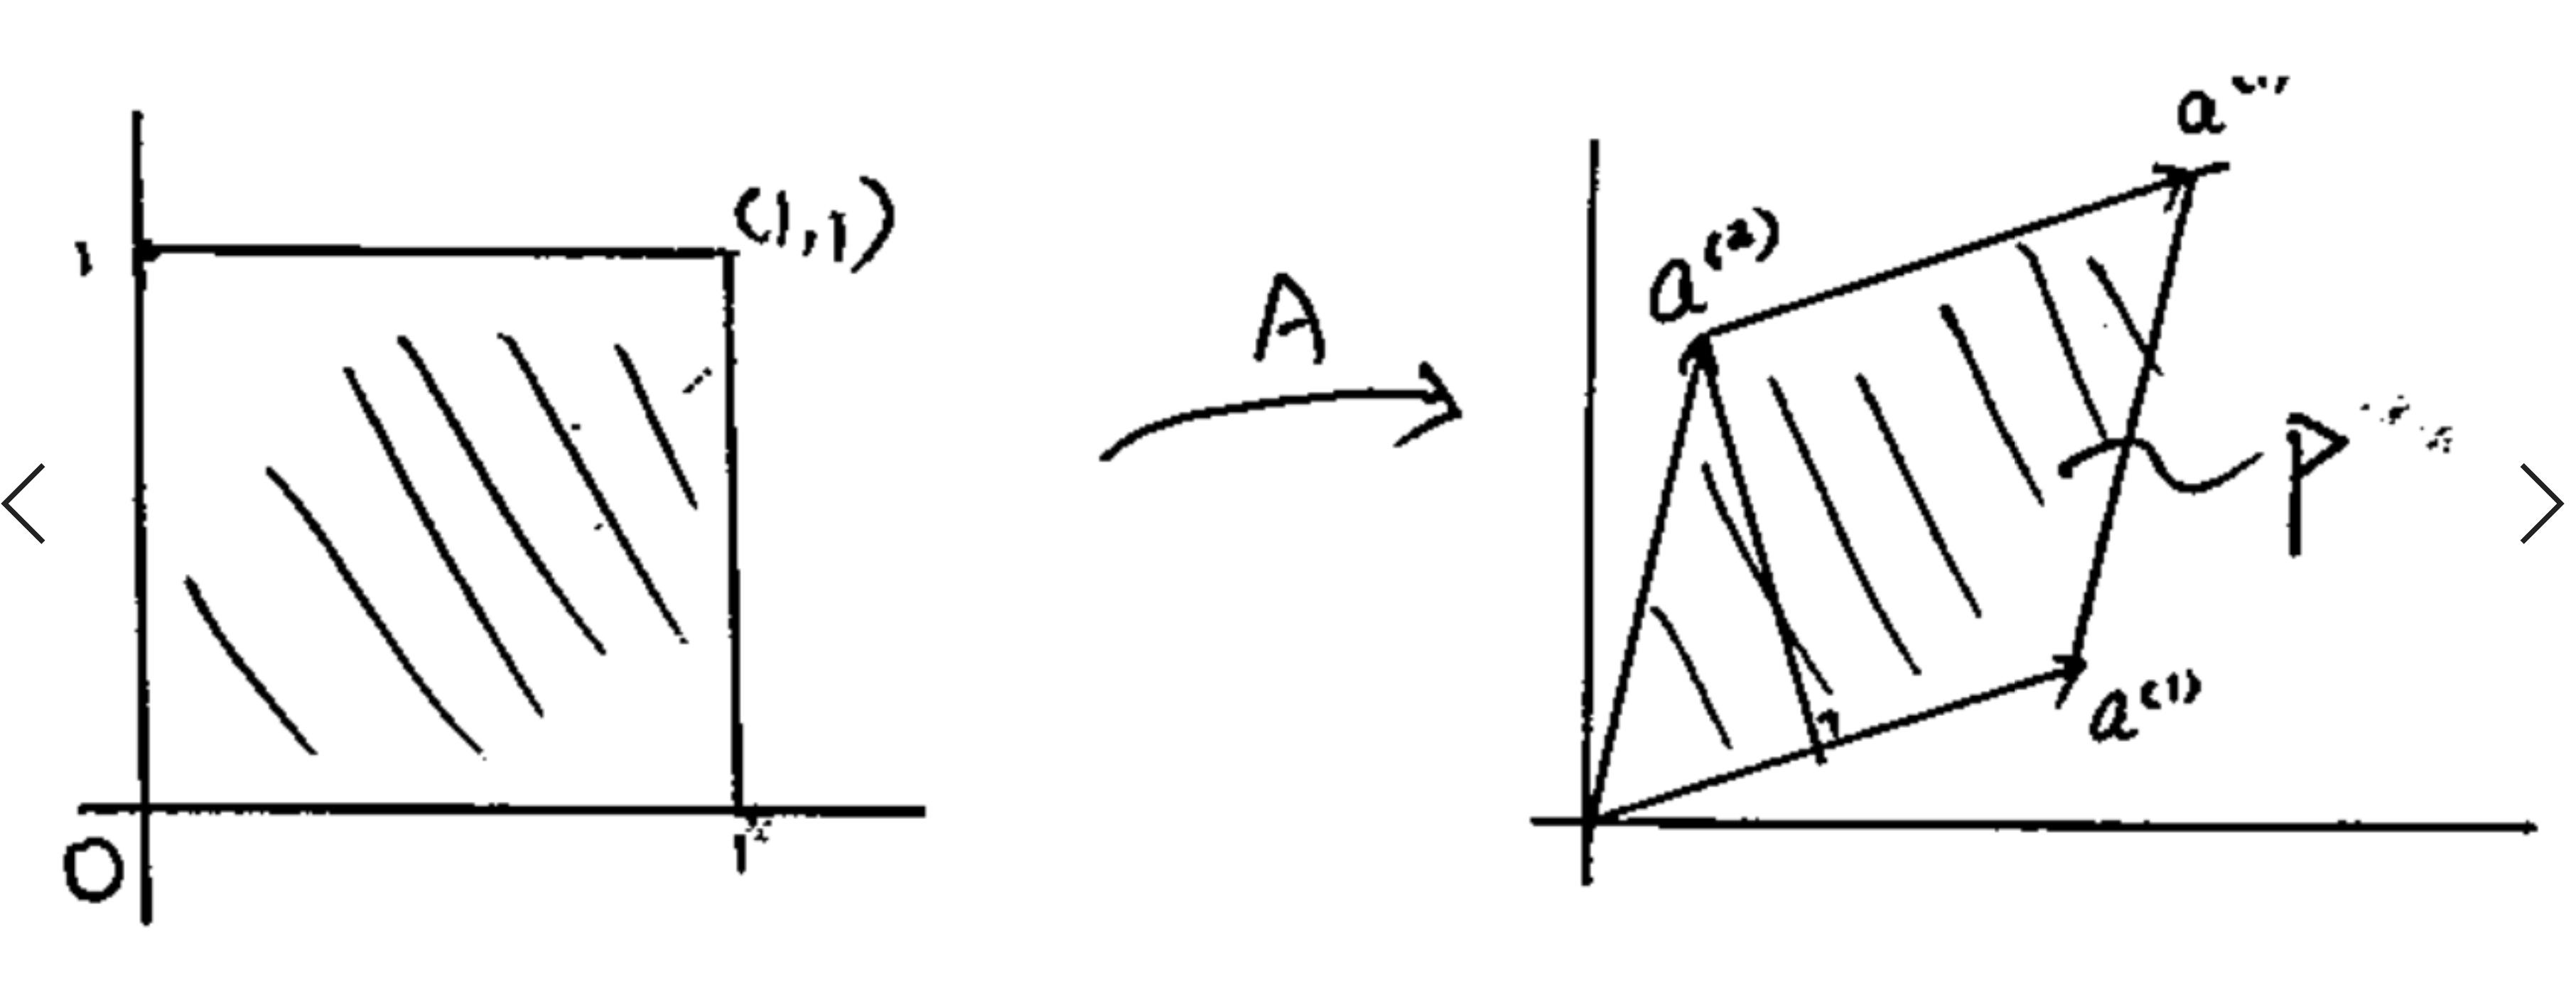
\includegraphics[width=2.1in,height=2.1in]{figures/ch03/figure1.jpg}
	%\caption{This is an inserted JPG graphic} 
	%\label{fig:graph} 
\end{figure}


Two matrices $A, B \in \Re^{n, n}$ are said to be \textbf{similar} if there exists a nonsingular matrix $P\in \Re^{n,n}$ s.t.:

\begin{equation*}
B = P^{-1}AP
\end{equation*}

Because there exists vectors $\tilde{x}, \tilde{y}$ s.t.:
\begin{align}
x &= P\tilde{x}\\
y &= P\tilde{y}\\
P\tilde{y} &= A P\tilde{x}\\
\tilde{y} &= P^{-1}AP P\tilde{x} = B \tilde{x}
\end{align}

Assume $A$ is \textbf{diagonalizable}(similar to a diagonal matrix):

\begin{align*}
A &= U\Lambda U^{-1}\\
|det(A)| &= |det(U\Lambda U^{-1})| \\
&= |det(U)det(\Lambda)det(U^{-1})|\\
&= det(U)det(\Lambda)\frac{1}{det(U)}\\
&= |det(\Lambda)|\\
&= |\prod^n_{i=1}\lambda_i|
\end{align*}

\begin{align*}
X: N(\mu, \Sigma)\,\,where\,\,(\mu \in \Re^n, \Sigma \in \Re^{n\times n})\\
P_x(x) = \frac{1}{(2\pi)^{\frac{2}{n}}}\frac{1}{|det\Sigma|^{\frac{1}{2}}}exp[-\frac{1}{2}(x - \mu)^T\Sigma^{-1}(x - \mu)]
\end{align*}



\chapter{Symmetric matrices and spectral decomposition}
\label{ch.symmMat}
%% Placeholder for chapter on symmetric matrices and spectral decomposition


\chapter{Singlar value decomposition}
\label{ch.SVD}
%% Placeholder for chapter on SVD
%% Placeholder for chapter on SVD
\section{The Singular Value Decomposition(SVD)}

\subsection{Eigen-decomposition}

For any $A\in \Re^{n\times n}$ that is diagonalizable, can express $A$ as 
\begin{equation*}
A = U\Lambda U^{-1}
\end{equation*}

$U$: Matrix of linear independent eigenvectors $\in \mathbb{C}^n$

$\Lambda$: Diagonal matrix of eigenvalues $\lambda_i\in \mathbb{C}$.

\subsection{Spectral}

For any $A\in S^n$ can express A as
\begin{equation*}
A = U\Lambda U^T
\end{equation*}

$U$: Orthogonal matrix ($\perp$ \& normalized) $U^{(i)}\in \Re^n$;

$\Lambda$: Diagonal matrix of $\lambda_i \in \Re$.

\subsection{SVD}

Any matrix $A\in \Re^{m\times n}$ can be expressed as 
\begin{equation*}
A =U\tilde{\Sigma} V^T
\end{equation*}



$U\in \Re^{m\times m}$: orthogonal so $UU^T =U^TU = I_m$

$V\in \Re^{n\times n}$: orthogonal so $VV^T = V^TV =I_n$

$$\tilde{\Sigma} = 
\left[
\begin{matrix}
\Sigma & \textbf{0}\\
\textbf{0}&\textbf{0}
\end{matrix}
\right]\in \Re^{m\times n}
$$

where $\Sigma = diag(\sigma_1,...,\sigma_r)\geq 0$

Comments:

SVD: 

\begin{itemize}
	\item inherits $\perp$ matrices of spectral decomp and purely real $\lambda_i$
	
	\item Generalizes to non-square matrices
	
	\item Loose property of direction invariance of eigen-decomposition
	
	\item Consider $Ax = U\Sigma V^Tx$. 
\end{itemize}

\begin{example}
	$y = Ax = U\tilde{\Sigma} V^Tx$
	
	$$U = 
	\left[
	\begin{matrix}
	\frac{1}{\sqrt{3}}&\frac{1}{\sqrt{2}} & \frac{1}{\sqrt{6}}\\
	\frac{1}{\sqrt{3}}&-\frac{1}{\sqrt{2}} & \frac{1}{\sqrt{6}}\\
	\frac{1}{\sqrt{3}}&0 & -\frac{2}{\sqrt{6}}
	\end{matrix}
	\right] \Sigma = 
	\left[
	\begin{matrix}
	2&0\\
	0&0\\
	0&0
	\end{matrix}
	\right] V = 
	\left[
	\begin{matrix}
	-\frac{1}{\sqrt{2}}&\frac{1}{\sqrt{2}}\\
	\frac{1}{\sqrt{2}}&\frac{1}{\sqrt{2}}
	\end{matrix}
	\right] A = 
	\left[
	\begin{matrix}
	-\frac{2}{\sqrt{6}}&\frac{2}{\sqrt{6}}\\
	-\frac{2}{\sqrt{6}}&\frac{2}{\sqrt{6}}\\
	-\frac{2}{\sqrt{6}}&\frac{2}{\sqrt{6}}
	\end{matrix}
	\right]
	$$
	$$ a) x = 
	\left[
	\begin{matrix}
	1\\
	0
	\end{matrix}
	\right]
	$$
	\begin{figure}
		\centering
		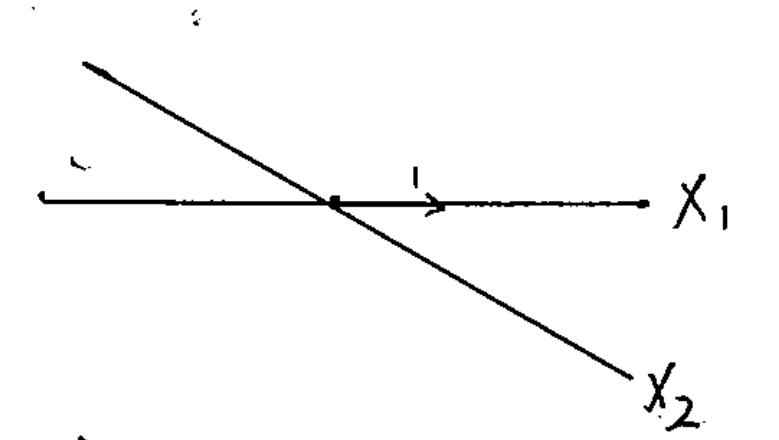
\includegraphics[width=2.1in,height=2.1in]{figures/ch05/figure1_a.jpg}
		%\caption{This is an inserted JPG graphic} 
		%\label{fig:graph} 
	\end{figure}
	$$ b) w = V^Tx = 
	\left[
	\begin{matrix}
	-\frac{1}{\sqrt{2}}\\
	\frac{1}{\sqrt{2}}
	\end{matrix}
	\right]
	$$
	\begin{figure}
		\centering
		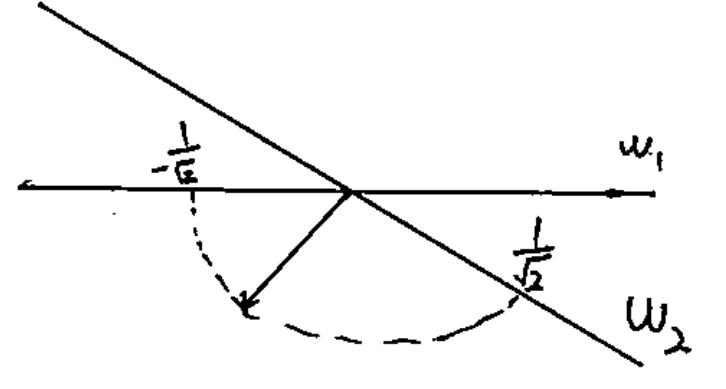
\includegraphics[width=2.1in,height=2.1in]{figures/ch05/figure1_b.jpg}
		%\caption{This is an inserted JPG graphic} 
		%\label{fig:graph} 
	\end{figure}
	$$ c) z = \Sigma w = 
	\left[
	\begin{matrix}
	-\frac{1}{\sqrt{2}}\\
	0\\
	0
	\end{matrix}
	\right]
	$$
	\begin{figure}
		\centering
		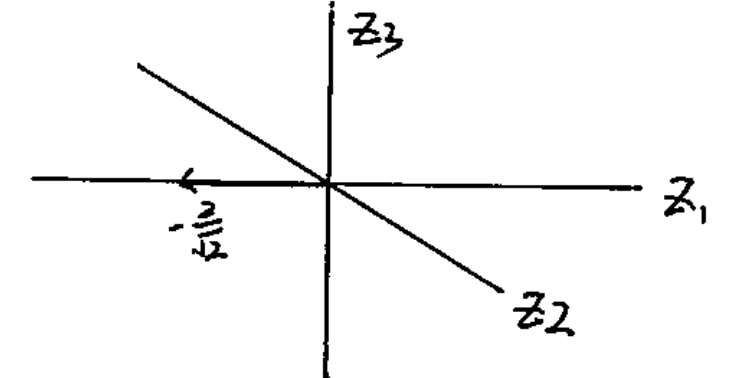
\includegraphics[width=2.1in,height=2.1in]{figures/ch05/figure1_c.png}
		%\caption{This is an inserted JPG graphic} 
		%\label{fig:graph} 
	\end{figure}
	$$ d) y = Uz =  
	\left[
	\begin{matrix}
	-\frac{2}{\sqrt{6}}\\
	-\frac{2}{\sqrt{6}}\\
	-\frac{2}{\sqrt{6}}
	\end{matrix}
	\right]
	$$
	\begin{figure}
		\centering
		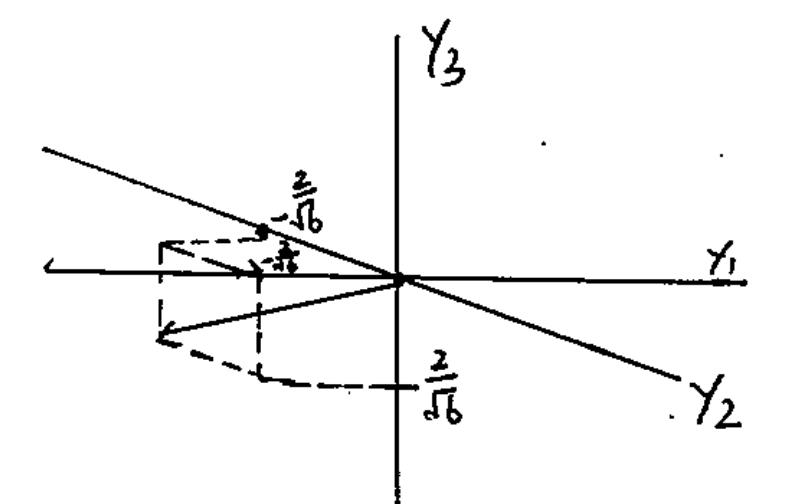
\includegraphics[width=2.1in,height=2.1in]{figures/ch05/figure1_d.jpg}
		%\caption{This is an inserted JPG graphic} 
		%\label{fig:graph} 
	\end{figure}
	
	
\end{example}


SVD follows from eigen-decomp of $A^TA$ and $AA^T$ $\rightarrow$ both symmetric, so spectral theorem applies. 

Write out $U\& V$ as: (r: rank($A$))



$$ U =   
\left[
\begin{matrix}
U^{(1)} & ... & U^{(r)} & U^{(r+1)} & ... & U^{(m)}
\end{matrix}
\right] =
\left[
\begin{matrix}
U_r & U_{mr}
\end{matrix}
\right]
$$


$$ V =   
\left[
\begin{matrix}
V^{(1)} & ... & V^{(r)} & V^{(r+1)} & ... & V^{(n)}
\end{matrix}
\right] =
\left[
\begin{matrix}
V_r & V_{nr}
\end{matrix}
\right]
$$




\begin{align*}
AA^T &= U\tilde{\Sigma} V^TV\tilde{\Sigma}^TU^T
&=
\begin{bmatrix}
\mathcal{U}_r & \mathcal{U}_{mr}
\end{bmatrix}
\begin{bmatrix}
\Sigma & \textbf{0}\\
\textbf{0}&\textbf{0}
\end{bmatrix}
\begin{bmatrix}
\Sigma^r & \textbf{0}\\
\textbf{0}&\textbf{0}
\end{bmatrix}
\begin{bmatrix}
\mathcal{U}_r^T\\
\mathcal{U}_{mr}^T
\end{bmatrix}
&=
\begin{bmatrix}
\mathcal{U}_r & \mathcal{U}_{mr}
\end{bmatrix}
\begin{bmatrix}
\Sigma^2 & \textbf{0}\\
\textbf{0}&\textbf{0}
\end{bmatrix}
\begin{bmatrix}
\mathcal{U}_r^T\\
\mathcal{U}_{mr}^T
\end{bmatrix}
&= \sum^r_{i=1}(\sigma_i)^2u^{(i)}(u&{(i)})^T\\
&= \sum^m_{i=1}(\sigma_1)^2u^{(i)}u^{(i)^T}
\end{align*}



$(AA^T)u^{(k)}$, $\rightarrow$ WTS $u^{(k)}$ is $k^{th}$ eigenvector of $AA^T$. 

$(AA^T)u^{(k)} = \sum^m_{i=1}\sigma_i^2u^{(1)}(u^{(1)})^Tu^{(k)} = \sum^n_{i=1}\sigma_i^2\prod(i=k)u^{(1)} =\sigma^2_ku^{(k)}$

$\lambda_k(AA^T) = \sigma^2_k$

same logic applied to $A^TA$ shows $V^{(k)}$ is $k^{th}$ eigenvector of $(A^TA)$


\subsection{Computing SVD}

1) Singular values: Compute eigenvalues of $AA^T$ or $A^TA$ to find $\lambda_i(A^TA) =\sigma_i^2$ $\rightarrow$ $\sigma_i = \sqrt{\lambda_i(A^TA)}$

$x^TA^TAx = w^Tw =||w||^2$

2) Right-Singular vectors: eigenvectors of $A^TA$;

3) Left-Singular vectors: eigenvectors of $AA^T$;

4) Because $AA^T \& A^TA$ both symmetric, both have full set of eigenvectors.\\

2. Consider arbitrary $x\in \Re^n$, 

\begin{align*}
Ax &= U\tilde{\Sigma} V^Tx\\
&= 
\begin{bmatrix}%
U_r & U_{mr}
\end{bmatrix}
\begin{bmatrix}%
\Sigma & \textbf{0}\\
\textbf{0}& \textbf{0}
\end{bmatrix}
\begin{bmatrix}%
V_r^T\\
V_{mr}^T
\end{bmatrix}x\\
&= 
\begin{bmatrix}%
U_r & U_{mr}
\end{bmatrix}
\begin{bmatrix}%
\Sigma\\
\textbf{0}
\end{bmatrix}
\begin{bmatrix}%
V_r^T
\end{bmatrix}x\\
&= \Sigma^r_{i=1}\sigma_iu^{(i)}(V^{(1)})^Tx (***)
\end{align*}
\\

Eq(*) looses all components of $x$ along $V^{(i)}$ directions when $r+1 \leq i \leq n$:

$\rightarrow$ i.e. columns of $V_{nr}$

$\rightarrow$ columns of $V_{nr}$ provide basis for $N(A)$.\\


All direction in output are in span $\{u^{(1)} ,..., u^{(n)}\}$

$\rightarrow$ columns of $U_r$ provide basis for $R(A)$.\\

Columns of $U_{mr}$ provide basis for $N(A^T)$\\

Columns of $V_{r}$ provide basis for $R(A^T)$


2) Consider arbitrary $x\in \Re^n$

\begin{align*}
A &= \mathcal{U}\tilde{\Sigma}V^r\\
&= 
\begin{bmatrix}
\mathcal{U}_r & \mathcal{U}_{mr}
\end{bmatrix}
\begin{bmatrix}
\Sigma & \mathbf{0}\\
\mathbf{0} & \mathbf{0}
\end{bmatrix}
\begin{bmatrix}
V_r^T\\
V_{nr}^T
\end{bmatrix}\\
&= 
\begin{bmatrix}
\mathcal{U}_r & \mathcal{U}_{mr}
\end{bmatrix}
\begin{bmatrix}
\Sigma \\
\mathbf{0} & 
\end{bmatrix}
\begin{bmatrix}
V_r^T
\end{bmatrix}\\
&= \mathcal{U}_r\Sigma V_r^T\\
\mathcal{U}_r^TAV_r &= \mathcal{U}_r^T(\mathcal{U}_r\Sigma V_r^T)V_r = \Sigma = \mathcal{U}_r^TAV_r
\end{align*}


\begin{align}
A &= \mathcal{U}_r\Sigma V_r^T \\
&= \sum^r_{i=1}\mathcal{U}^{(i)}(V^{(i)})^T\sigma_i\\
&= \sigma_1\mathcal{U}^{(1)}V^{(1)^T}+ \sigma_2\mathcal{U}^{(2)}V^{(2)^T}
\end{align}

\begin{equation*}
\sigma_1\mathcal{U}V^{(1)^T} = 
\begin{bmatrix}
\sigma_1V_1^{(1)}\mathcal{U}^{(1)} & \sigma_1V_2^{(1)}\mathcal{U}^{(1)} & ... & \sigma_1V_n^{(1)}\mathcal{U}^{(1)}
\end{bmatrix}
\end{equation*}

Condition \#

Consider $Ax = b$ when $A$ is invertible, solve for $x$ as $x = A^{-1}b$. What if $b = b_r + e$? how much does solution change? 

Solution is $\hat{x} = A^{-1}b_T + A^{-1}e$

\begin{equation*}
\frac{||\frac{A^{-1}e||}{||A^{-1}b_T||}}{\frac{||e||}{||b||}} = \frac{||A^{-1}e||_2}{||e||_2} \frac{||b||_2}{||A^{-1}b||_2}
\end{equation*}

\begin{align*}
max_{e,b\neq 0} \, \frac{||A^{-1}e||}{||e||} \frac{||b||}{||A^{-1}b||} &= \left[max_{e\neq 0}\, \frac{||A^{-1}e}{||e||}\right]\left[max_{b\neq 0}\, \frac{||b||}{||A^{-1}b||}\right]\\
&= \frac{\sigma_{max}(A^{-1})}{\sigma_{min}(A^{-1}}\\
&= \frac{\frac{1}{\sigma_n}}{\frac{1}{\sigma_1}}\\
&= \frac{\sigma_1}{\sigma_n}\\
&= \frac{\sigma_{max}(A)}{\sigma_{min}(A)}
&= K(A)
\end{align*}

\begin{figure}
	\centering
	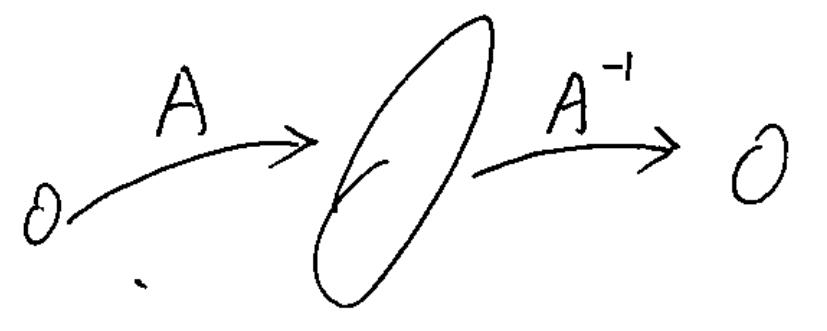
\includegraphics[width=2.1in,height=2.1in]{figures/ch05/figure2.jpg}
	%\caption{This is an inserted JPG graphic} 
	%\label{fig:graph} 
\end{figure}

\begin{align}
A^{-1} &= (\mathbb{U}\Sigma V^T)^{-1} \\
&= V\Sigma^{-1}\mathcal{T}\\
&= V
\begin{bmatrix}
\frac{1}{\sigma_1} & &\\
& ... & \\
& & \frac{1}{\sigma_n}
\end{bmatrix}
\mathcal{U}^T\\
\sigma_{max}(A^{-1}) = \frac{1}{\sigma_n}\\
\sigma_{min}(A^{-1}) = \frac{1}{\sigma_1}
\end{align}


\chapter{Linear equations and least squares}
\label{ch.linEqLS}
%% Placeholder for chapter on linear equations and least squares
%%%zhipeng add the following part
%% Placeholder for chapter on linear equations and least squares




\section{Least Squares}
Consider the linear system
\begin{equation*}
Ax = y \qquad (*)
\end{equation*}
where $A\in \reals^{m\times n}$ is the coefficient data matrix (known), $y\in \reals^m$ are constraints(known) and $x\in \reals^n$ are unknown parameters that we need to figure out.

There are three possibilities for the solution of this system:

a) No $x\in \reals^n$ satisfies ($*$) 
	
b) An unique $x\in \reals^n$ satisfies ($*$) 
	
c) Many $x\in \reals^n$ satisfies ($*$) 

\vspace{0.3cm}
Since $Ax\in R(A)$, a solution $x$ will exist if $y\in R(A)$.

There is a simple test based on the ranks of augmented matrix and coefficient matrix:

1) $\rank(A) = \rank\left([A\ y] \right)$: solution to ($*$) exists

2) $\rank(A) < \rank\left([A\ y] \right)$: no solution to ($*$) exists

\vspace{0.4cm}
Suppose there exist a solution, the next question is, is it unique?

Assume a solution $\bar{x}$ exists such that $A\bar{x} = y$ (i.e., a particular solution), and there may have other solution $x$ also satisfy $Ax = y$. Therefore, we can write
\begin{align*}
Ax - A\bar{x} &= A(x -\bar{x}) = 0\\
x - \bar{x} &\in N(A)
\end{align*}

That is, any solution to ($*$) can be expressed as a sum of a particular solution plus a trival solution of, i.e.,
\begin{equation*}
x = \bar{x} + (x - \bar{x}) = \bar{x} + e
\end{equation*}
where $e\in N(A)$ (i.e., a solution to the homogeneous case $Ax = 0$).

So if there are many solutions to ($*$), we will have a affine sets given by
\begin{equation*}
\mathcal{A} = \{x|x = \bar{x} + N(A), A\bar{x} = y \}
\end{equation*}

Now, from this point of view, we could say that the solution $\bar{x}$ is unique if the elements of $N(A)$ are all zero(there is only a trival solution $e$ satisfy $Ax=0$, that is, $e$ is a zero vector), and $\bar{x}$ is any particular solution for $A\bar{x} =y$.

\vspace{0.5cm}
The three case regarding the solution of a linear system typically bread down into a question about dimensions of $A\in \reals^{m\times n}$. The results are summarized as follows
\begin{itemize}
	\item 1) Overdetermined linear system: $m>n$, more constraints than unknown parameters. Typically a solution does not exist (holds when $m$ equations are linearly independent).
	
	\item 2) Square: $m=n$, equal number of constraints and parameters, and typically there exists a unique solution.
	
	\item 3) Underdetermined linear system: $m<n$, fewer constraints than parameters, and typically many solutions exists.
\end{itemize}

\vspace{0.3cm}
\subsection{Overdetermined linear system : $m > n$ }


Assume $A$ is full column rank(i.e., full rank), $\rank(A) =n$. Therefore, $A$ is a tall and thin matrix, and $\dim(R(A)) = n < m$.

Suppose we have $m$ independent equations with $m>n$, and in this case there is no exact solution to $(*)$ (in fact this conclusion holds if there are at least $n+1$ equations are independent). This case is very commonly meet in reality, and thus we want to find a $x^*$ such that $Ax^*$ is the 'closest' to $y$, that is, to solve the following optimization problem
$$x^* = \arg \min_{x\in \reals^n}\Vert Ax - y\Vert_2$$

Note that $Ax \in R(A)$, and from the perspective of projection, we could rewrite the problem as
$$\min_{x\in \reals^{n}}||Ax - y\Vert_2 = \min_{\hat{y}\in R(A)}\Vert \hat{y} - y\Vert_2 =\prod_{R(A)}(y)$$
and this problem becomes find a projection of $y$ in the column space of $A$.

\begin{marginfigure}
	\centering
	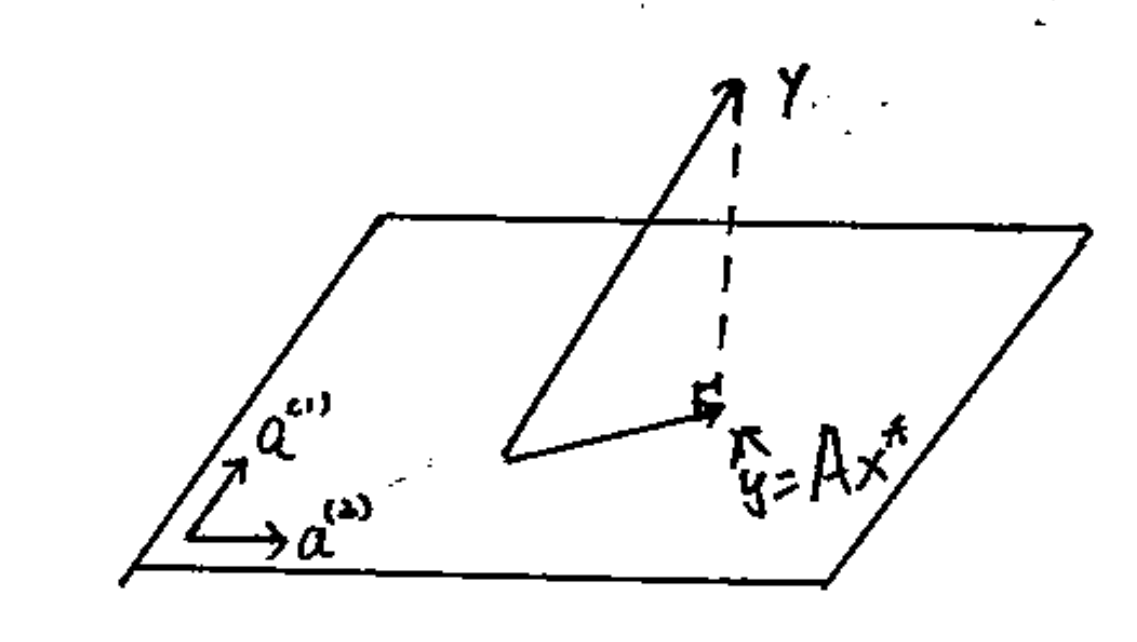
\includegraphics[width=2.1in,height=2.1in]{figures/ch06/figure1.png}
	%\caption{This is an inserted JPG graphic} 
	%\label{fig:graph} 
\end{marginfigure}

From chapter2, we know that the projection of $y$, $\hat{y}^*$, can be expressed as
\begin{equation*}
\hat{y}^* = Ax^*= \sum^n_{i=1}x_i^*a^{(i)}
\end{equation*}
where 
$A =   
\left[
\begin{matrix}
a^{(1)} & \cdots & a^{(n)}
\end{matrix}
\right]
$.

Recall what we have done before, we could solve for $x^*$ via a bunch of equations(i.e., solve for each $x_i^*$),
\begin{equation*}
\sum^n_{i=1}x_i^*\langle a^{(k)}, a^{(i)}\rangle = \langle a^{(k)}, y\rangle, \quad \forall k= 1,2,\cdots,m
\end{equation*}

For convenience, we could stack up to get what we called the normal equation:
\begin{equation*}
A^{\trans}Ax^* = A^{\trans}y
\end{equation*}

There are 2 possibilities: 

(a) $A^{\trans}A$ is invertible (this holds when $A$ has full column rank, which we have assumed in the beginning):
\begin{align*}
x^* &= (A^{\trans}A)^{-1}A^{\trans}y\\
\hat{y}^* &= A(A^{\trans}A)^{-1}A^{\trans}y
\end{align*}


(b) $A^{\trans}A$ is not invertible (if we do not assume that $A$ has full column rank):

We apply SVD to $A^{\trans}$ and  $A$:
\begin{align*}
\hat{y}^* &= A(A^{\trans}A)^{-1}A^{\trans}y\\
&= A(V
\begin{bmatrix}
\Sigma & \textbf{0}
\end{bmatrix}
\mathcal{U}^{\trans}\mathcal{U}
\begin{bmatrix}
\Sigma \\
\textbf{0}
\end{bmatrix}
V^{\trans})^{-1}A^{\trans}y\\
&= A(V\Sigma^2V^{\trans})^{-1}A^{\trans}y\\
&= AV(\Sigma^{-1})^2V^{\trans}A^{\trans}y\\
&= \mathcal{U}
\begin{bmatrix}
\Sigma \\
\textbf{0}
\end{bmatrix}
V^{\trans}V\Sigma^{-2}V^{\trans}V
\begin{bmatrix}
\Sigma & \textbf{0}
\end{bmatrix}
\mathcal{U}^{\trans}y\\
&= \mathcal{U}
\begin{bmatrix}
\Sigma \\
\textbf{0}
\end{bmatrix}
\Sigma^{-1}\Sigma^{-1}
\begin{bmatrix}
\Sigma & \textbf{0}
\end{bmatrix}
\mathcal{U}^{\trans}y\\
&= \mathcal{U}
\begin{bmatrix}
I_r\\
\textbf{0}
\end{bmatrix}
\begin{bmatrix}
I_r & \textbf{0}
\end{bmatrix}
\mathcal{U}^{\trans}y\\
&= \mathcal{U}
\begin{bmatrix}
I_r& \textbf{0}\\
\textbf{0} & \textbf{0}
\end{bmatrix}
\mathcal{U}^{\trans}y\\
&= \mathcal{U}
\begin{bmatrix}
I_r& \textbf{0}\\
\textbf{0} &  \textbf{0}
\end{bmatrix}
\begin{bmatrix}
\langle u^{(1)}, y\rangle\\
\langle u^{(2)}, y\rangle \\
\vdots\\
\langle u^{(m)}, y\rangle
\end{bmatrix}\\
&= \sum^r_{i=1}\langle u^{(i)}, y\rangle u^{(i)}
\end{align*}


\subsection{Uniquely determined: $m =n$}
Given the linear system with $m=n$
$$Ax = y$$

The solution is given by
$$x^* = A^{-1}y$$

Note that:

(a) There are equal number of constraints and parameters in this case.

(b) We assume that $A$ has full rank (both columns and rows).
	
(c) Since $A$ is a square matrix with full rank, $A^{-1}$ exists.



\subsection{Underdetermined linear system: $m<n$ }

Note that

	(a) Since $m<n$, $A$ is a wide and short matrix.
	
	(b) In this case, there are more parameters than constraints.
	
	(c) We assume that $A$ has full row rank, so $\rank(A) = m$
	
	(d) Hence, there are many solutions.

\vspace{0.3cm}

Since in this case, there are many solutions satisfy the linear equation $Ax=y$, then the idea to pick the optimal one is, we choose a solution $x$  with the shortest length in the sense of $L_2$ norm, that is, solve the following optimization problem
$$x^* = \arg  \min_{Ax = y, x\in \reals^n}\Vert x\Vert _2$$

Alternatively, we can rephrase the problem from the perspective of projection
\begin{equation*}
\min_{Ax = y, x\in \reals^n}\Vert x\Vert  = \min_{x\in \reals^n, x\in \mathcal{A}}\Vert x - 0\Vert  = \prod_{\mathcal{A}}(0)
\end{equation*}
since the set $\{x | Ax= y \}$ is an affine space. Therefore, the problem becomes finding the projection of origin from the affine space $\mathcal{A}$.



\begin{figure}
	\centering
	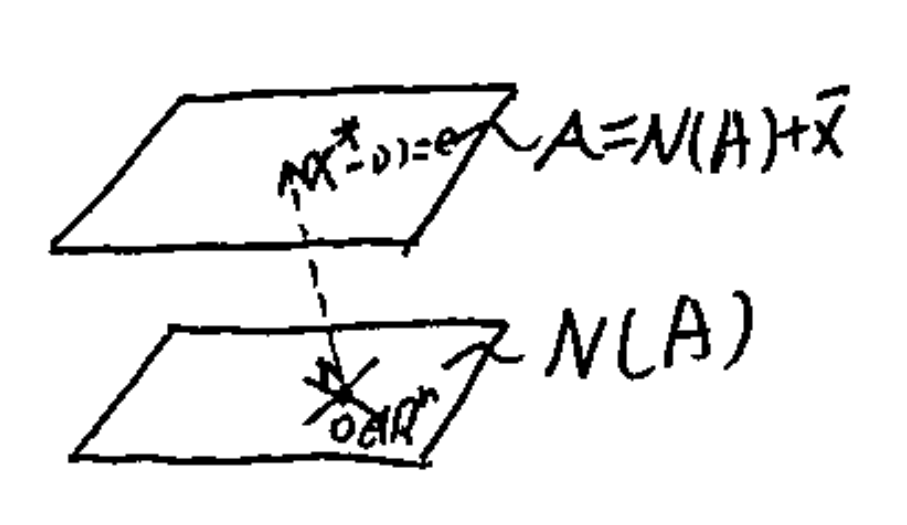
\includegraphics[width=1.6in,height=1.6in]{figures/ch06/figure3.png}
	%\caption{This is an inserted JPG graphic} 
	%\label{fig:graph} 
\end{figure}

To solve for $x^*$, note (from before) error vector 
\begin{align*}
e &= x^* - 0 = x^* \perp N(A)\\
x^* &\in N(A)^{\perp} = R(A^{\trans})
\end{align*}

So we can write $x^* = A^{\trans}\alpha$ for some $\alpha \in \reals^m$. For $x^*$ to be in $\mathcal{A}$ it must satisfy that $Ax^* = y$, substituting in we get 
\begin{equation*}
Ax^* = y= AA^{\trans}\alpha
\end{equation*}

By assumption, $A$ is full row rank so $AA^{\trans}$ is invertible, so 
$$\alpha = (AA^{\trans})^{-1}y$$

and the optimal solution is given by
$$x^* = A^{\trans} \alpha = A^{\trans}(AA^{\trans})^{-1}y$$

In addition, $A^{+} =A^{\trans}(AA^{\trans})^{-1}$ is  what we called the Moore–Penrose pseudo inverse of $A$ (and it is also the right inverse of $A$ provided $A$ has full row rank).

Furthermore, we apply SVD to $A$ and $A^{\trans}$,
\begin{align*}
x^* &= A^{\trans}(AA^{\trans})^{-1}y\\
&= A^{\trans}\left[\mathcal{U}
\begin{bmatrix}
\Sigma & \mathbf{0}
\end{bmatrix}
V^{\trans}V
\begin{bmatrix}
\Sigma\\
\mathbf{0}
\end{bmatrix}
\mathcal{U}^{\trans}\right]^{-1}y\\
&= A^{\trans}(\mathcal{U}\Sigma^2\mathcal{U}^{\trans})^{-1}y\\
&= A^{\trans}\mathcal{U}\Sigma^{-2}\mathcal{U}^{\trans}y\\
&= V
\begin{bmatrix}
\Sigma\\
\mathbf{0}
\end{bmatrix}
\mathcal{U}^{\trans}\mathcal{U}\Sigma^{-2}\mathcal{U}^{\trans}y\\
&=V
\begin{bmatrix}
\Sigma^{-1} \\
\mathbf{0}
\end{bmatrix}
\mathcal{U}^{\trans}y\\
&= V
\begin{bmatrix}
\Sigma^{-1}\\
\mathbf{0}
\end{bmatrix}
\begin{bmatrix}
\langle u^{(1)}, y\rangle\\
\vdots\\
\langle u^{(n)}, y\rangle
\end{bmatrix}\\
&= \sum^r_{i=1}\frac{1}{\sigma_i}\langle u^{(i)}, y\rangle v^{(i)}
\end{align*}





\vspace{0.3cm}
\subsection{Interpretation of $x^*= \arg \min_x \Vert y-Ax\Vert_2$}


\quad\ (1). Approximated solution to $y=Ax$

$y^*=Ax^*$ is the 'best' approximated solution in the sense of $L_2$ norm, which means, $y^*$ is the closest point in $R(A)$ to $y$.

(2). Minimum perturbation of $y$ to 'feasibility'

\begin{figure}
	\centering
	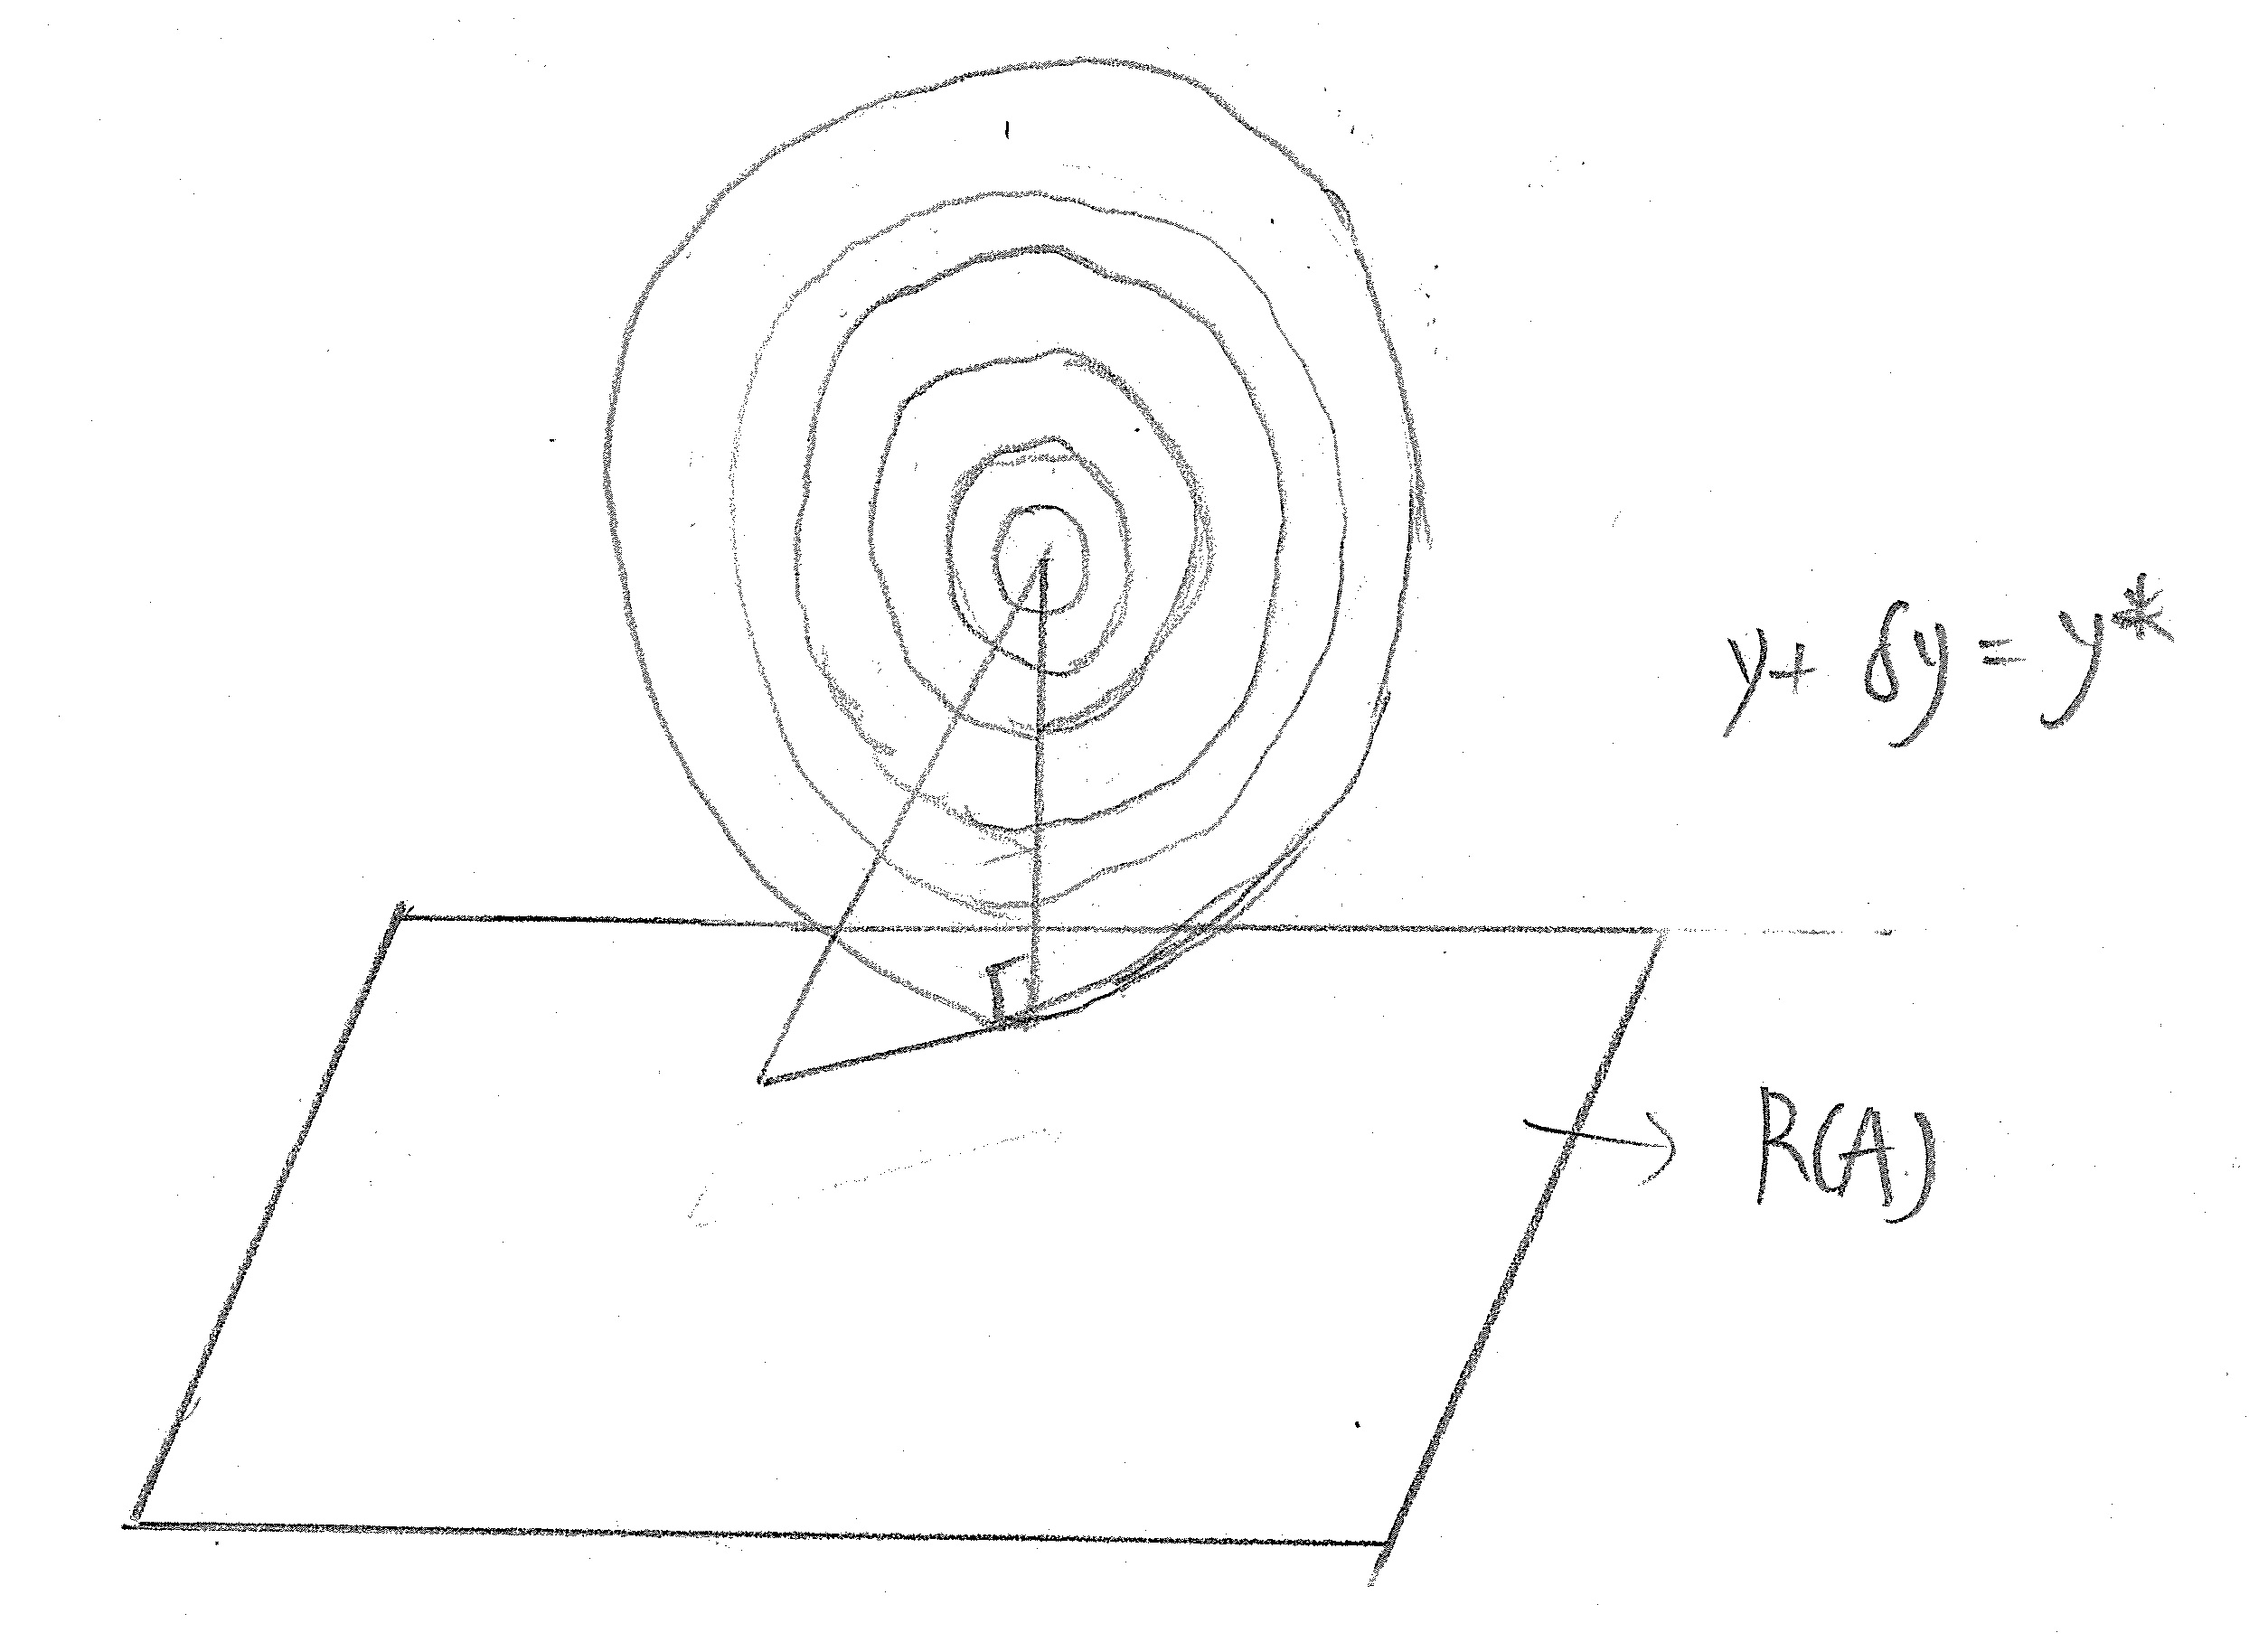
\includegraphics[width=2in,height=2in]{figures/ch06/ch06-01.jpg}
	%\caption{This is an inserted JPG graphic} 
	%\label{fig:graph} 
\end{figure}

(3). Perturb both $y$ and $A$ to get 'feasibility'

"Total least square"

Suppose there are only pertubation for $y$ but also pertubation of $A$, formally we want to solve the following optimization problem
\begin{align*}
\min_{\delta y,  \delta A} & \left\Vert [\delta A\ \delta y] \right\Vert_F \\
s.t.\quad& y +\delta y = (A + \delta A) x
\end{align*}
where $\delta A\in \reals^{m\times n}$, $\delta y \in\reals^m$,  and also $[\delta A\ \delta y]$ is a $m$ by $n+1$ matrix, $y+\delta y\in R(A+\delta A)$. To solve this problem, we may utilize SVD.


(4). Linear regression
$$\Vert y-Ax\Vert ^2_2 = \sum_{i=1}^{m} ( y_i - \langle a^{(i)} , x\rangle )^2 = \sum_{i=1}^{m} r_i^2$$
where $r_i$ defined as the residual, and thus the standard least square problem can also be interpreted as a problem of minimizing the sum of square of residuals.

\begin{figure}
	\centering
	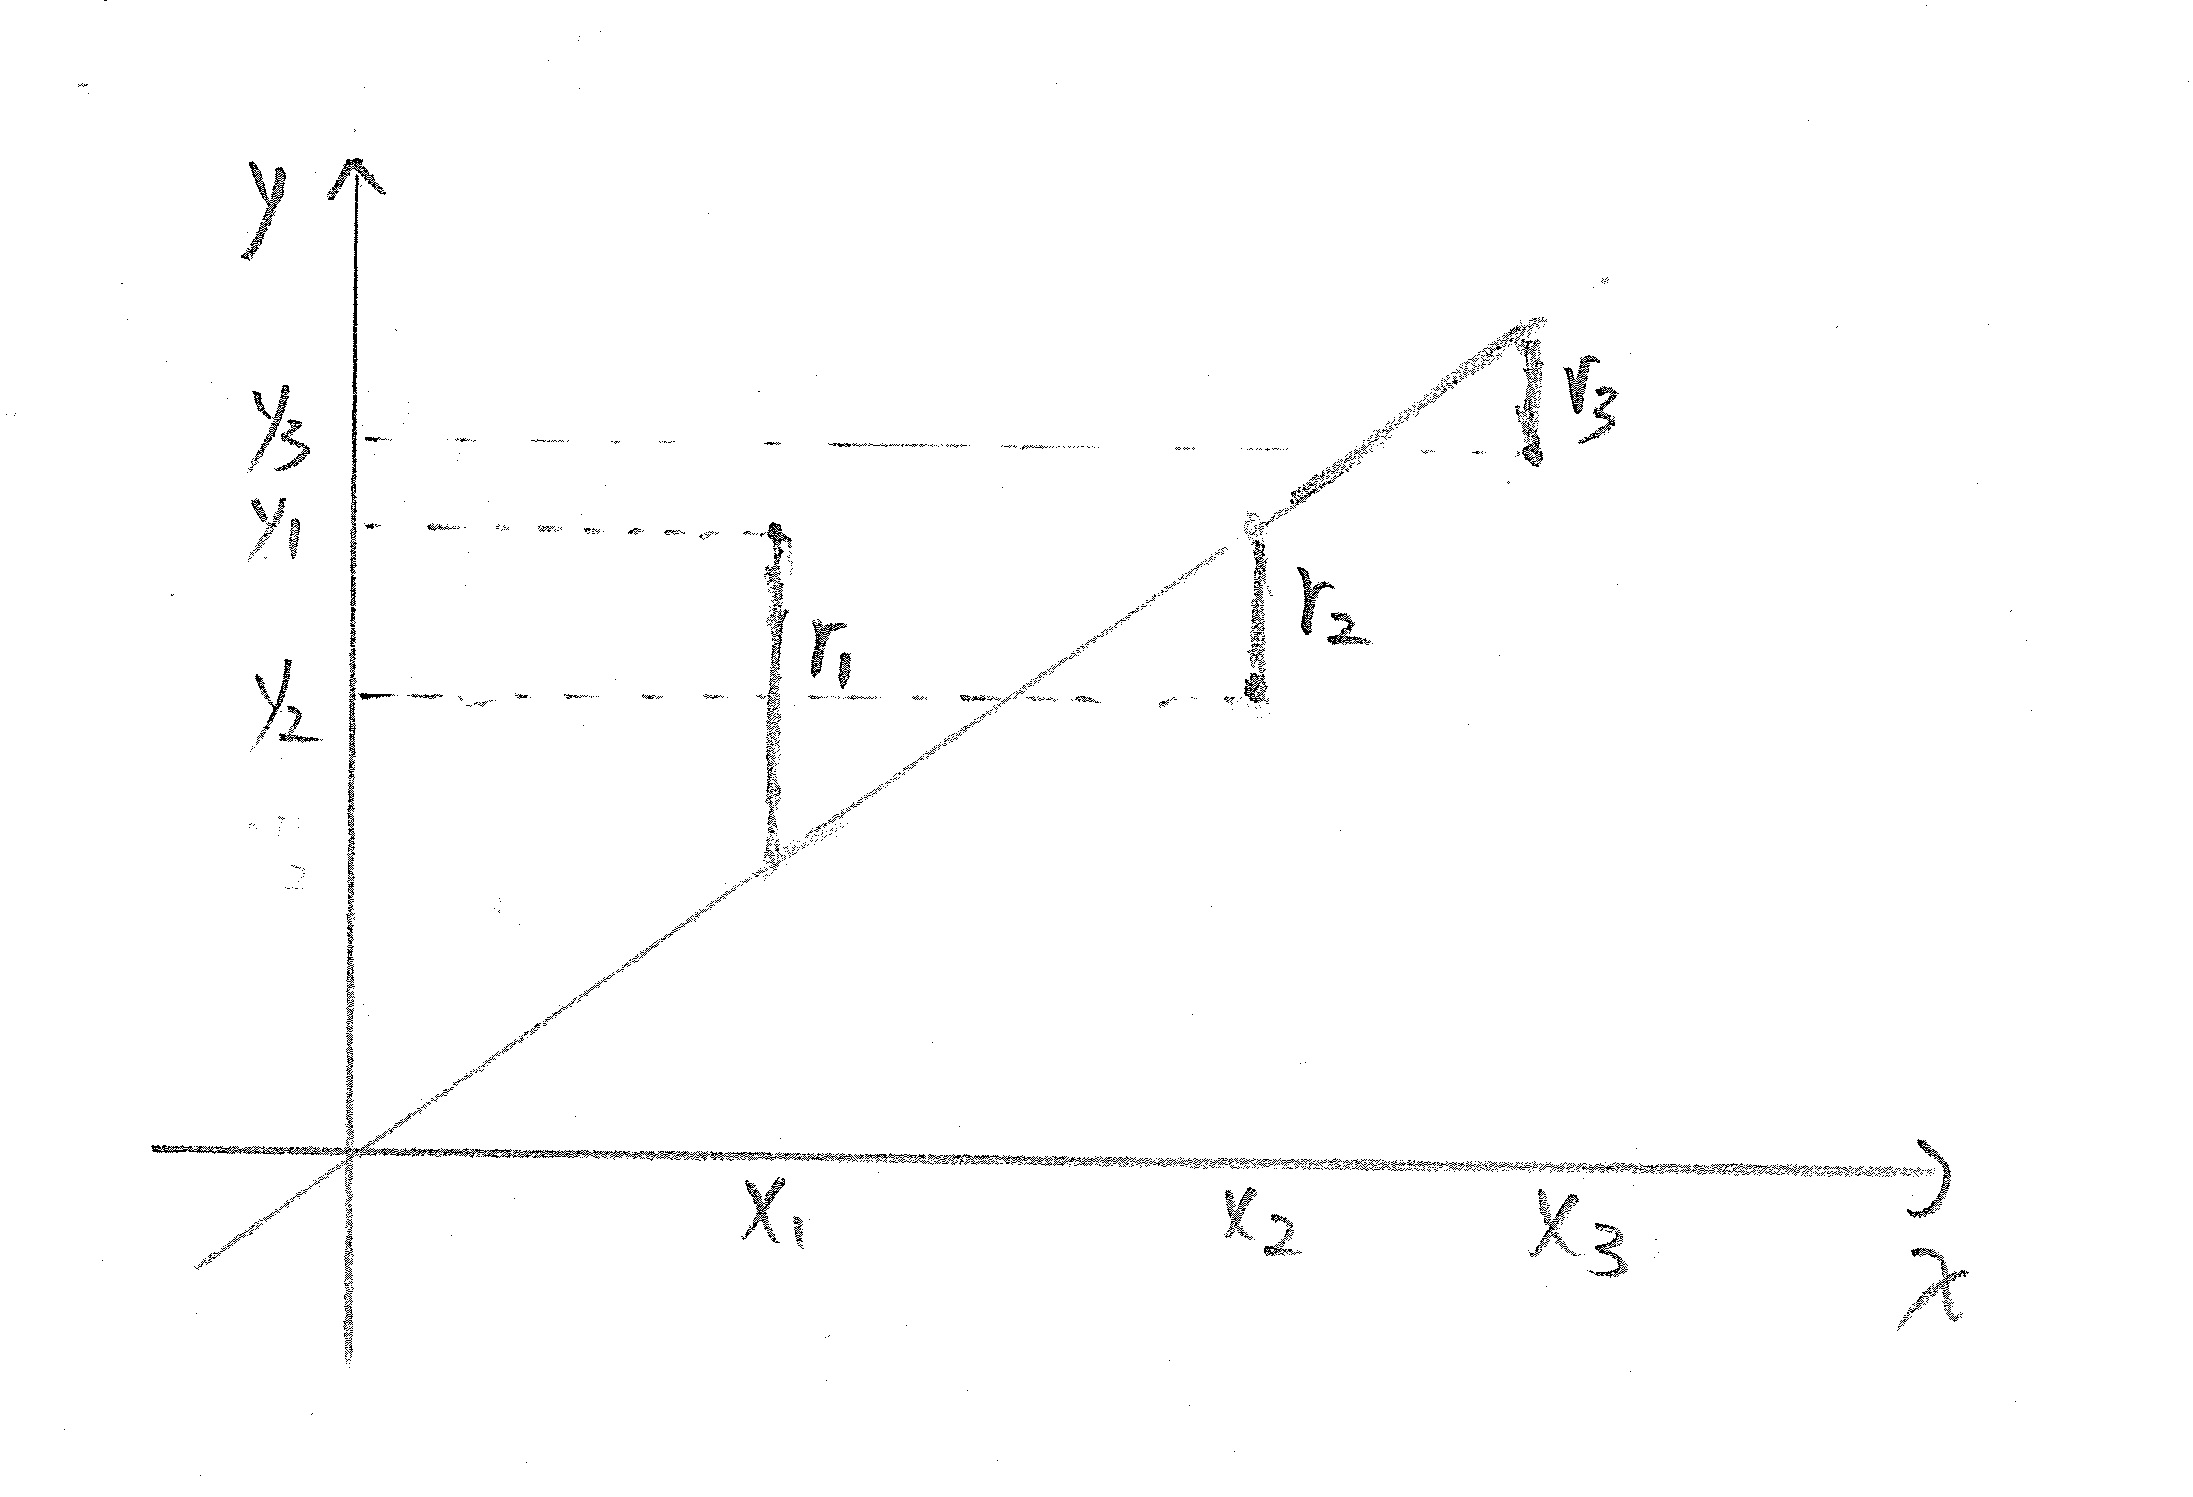
\includegraphics[width=2in,height=2in]{figures/ch06/ch06-02.jpg}
	%\caption{This is an inserted JPG graphic} 
	%\label{fig:graph} 
\end{figure}


\begin{example}

Let's consider fitting a line to $\{(0,6),(1,0),(2,0) \}={(a_i,y_i)}.$

The approximation takes the form of $y=x_1+ax_2$, and we want to choose a vector $x$ to minimize $\sum_{i=1}[y_i-(x_1+a_ix_2)]^2 = \sum_{i=1} r_i^2$, that is, we want to minimize the following
\begin{align*}
\Vert y- Ax\Vert_2^2 
&=
\left\Vert
\begin{bmatrix}
6\\
0\\
0
\end{bmatrix}
-
\begin{bmatrix}
1&0\\
1&1\\
1&2
\end{bmatrix}
\begin{bmatrix}
x_1\\
x_2
\end{bmatrix}
\right\Vert_2^2\\
&=\Vert y-Ax^*\Vert^2_2\\
&=6
\end{align*}

To solve for $x^*$, we have
$x^*=(A^{\trans}A)^{-1}A^{\trans}y=[5 , -3]^{\trans}$

Thus, the equation for this line is
$$\hat{y}^*=x_1^*+ax_2^*=5-3a$$            %so x1 and x2 are parameters

This example also illustrates that, if we would like to add an intercept term in the linear model, we could just let the first column of $A$ be an vector will all entries are $1$.
\end{example}


\section{Variants of least square}

\subsection{Weighted least square}
In the previous classical least square method, we do not consider the weights for each square of the residual(i.e., all of them are equally weighted), however, some residuals might be more important than the others. A very natural approach is to assign different weights to different $r_i^2$.

Formally, we formulate the optimization problem as
\begin{align*}
\min \sum_{i=1}^{n} w_i^2 r_i^2
&=\Vert W (y-Ax)\Vert ^2_2\\
&=\Vert Wy-WAx)\Vert ^2_2\\
&=\Vert \bar{y}-\bar{A}x \Vert ^2_2
\end{align*}
where $W=\diag(w_1, w_2, \cdots, w_m)$ and each $w_i\geq 0$, $\bar{y} \triangleq Wy$ and $\bar{A} \triangleq WA$. 

From the last two equities, we may find that this is very similar with the classic one but now we need to solve for $x$ in a transformed coordinate system.

To solve for $x^*$, we analogy to the solution of standard least square, and we have the normal equation
$$\bar{A}^{\trans} \bar{A} x=\bar{A}^{\trans} \bar{y}$$
so the solution is given by
$$x^*=(A^{\trans} W^{\trans} W A)^{-1} A^{\trans} W^{\trans} W y$$


In fact, if $W$ is positive definite(and thus $W^T W$ is positive definite), we can use a more general transform with PD, 
$$\Vert W (y-Ax)\Vert ^2_2 = (y-Ax)^{\trans}W^{\trans}W(y-Ax)=r^{\trans}W^{\trans}Wr$$
where $r$ is the residual in the original coordinate system, and we recognize that this objective is indeed an ellipsoid.

\newpage
\vspace{0.3cm}
Standard LS
\begin{figure}
	\centering
	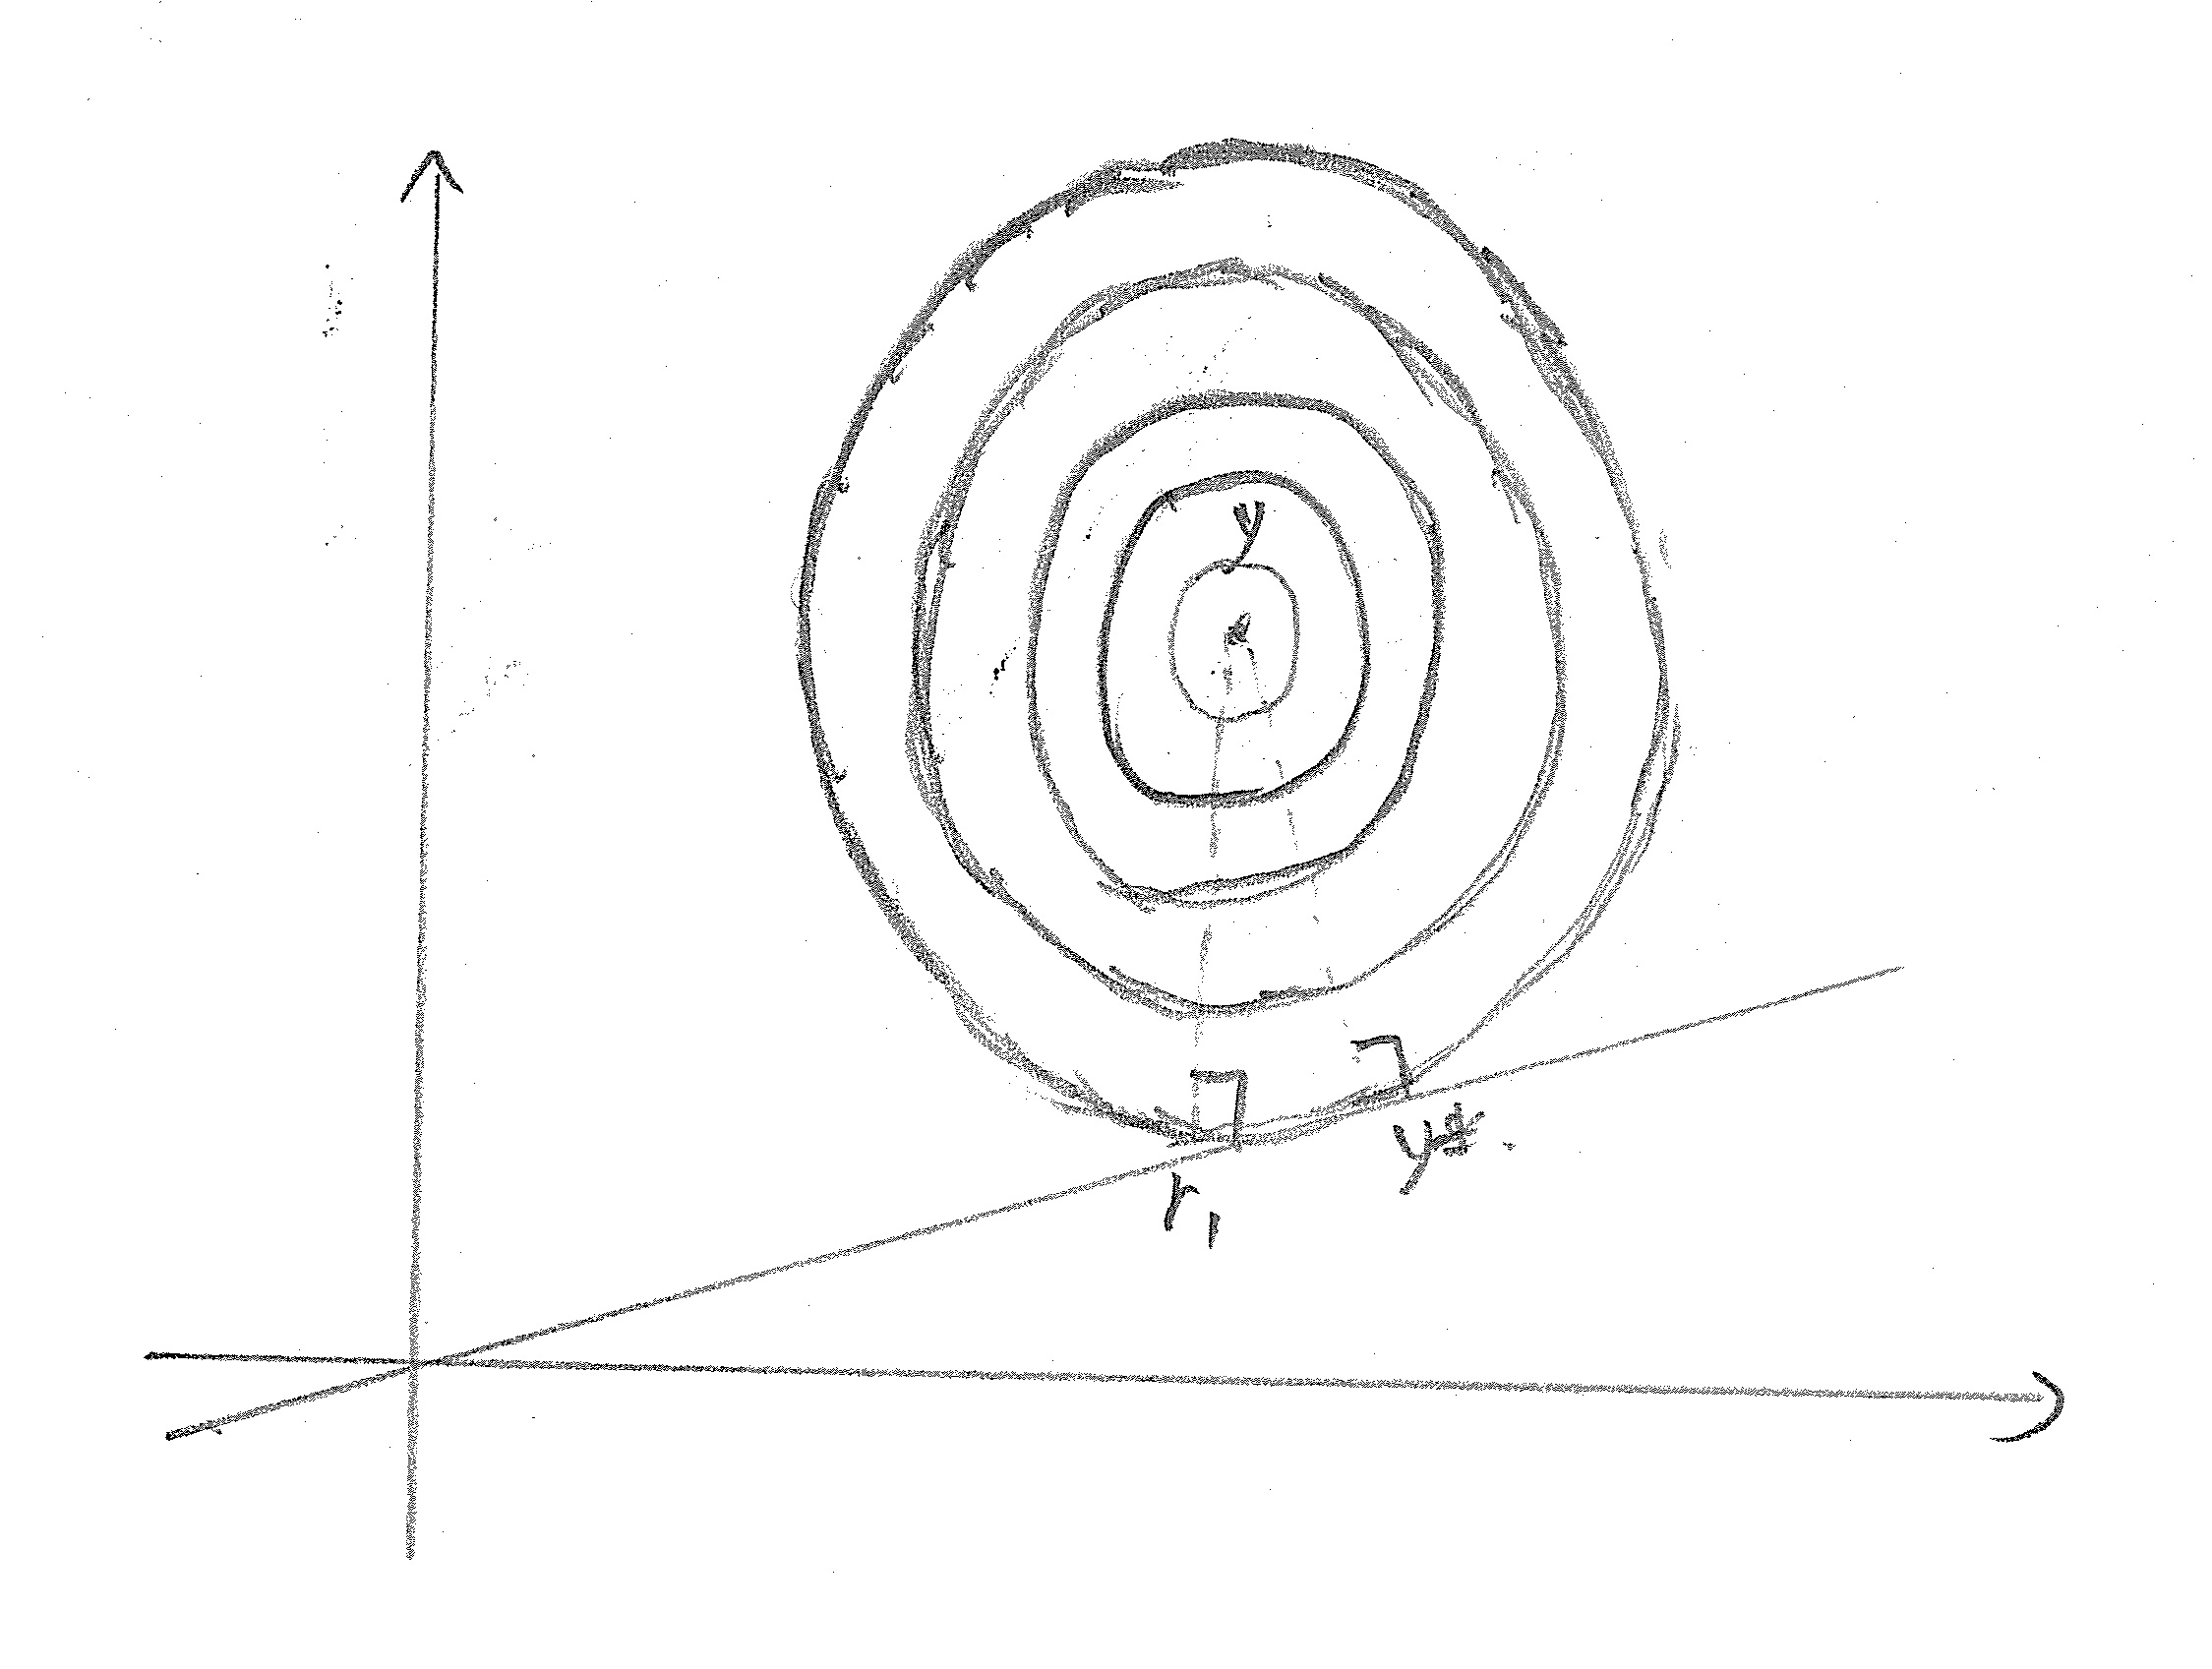
\includegraphics[width=2in,height=2in]{figures/ch06/ch06-03.jpg}
	%\caption{This is an inserted JPG graphic} 
	%\label{fig:graph} 
\end{figure}

Weighted LS with $W$ is diagonal 

\begin{figure}
	\centering
	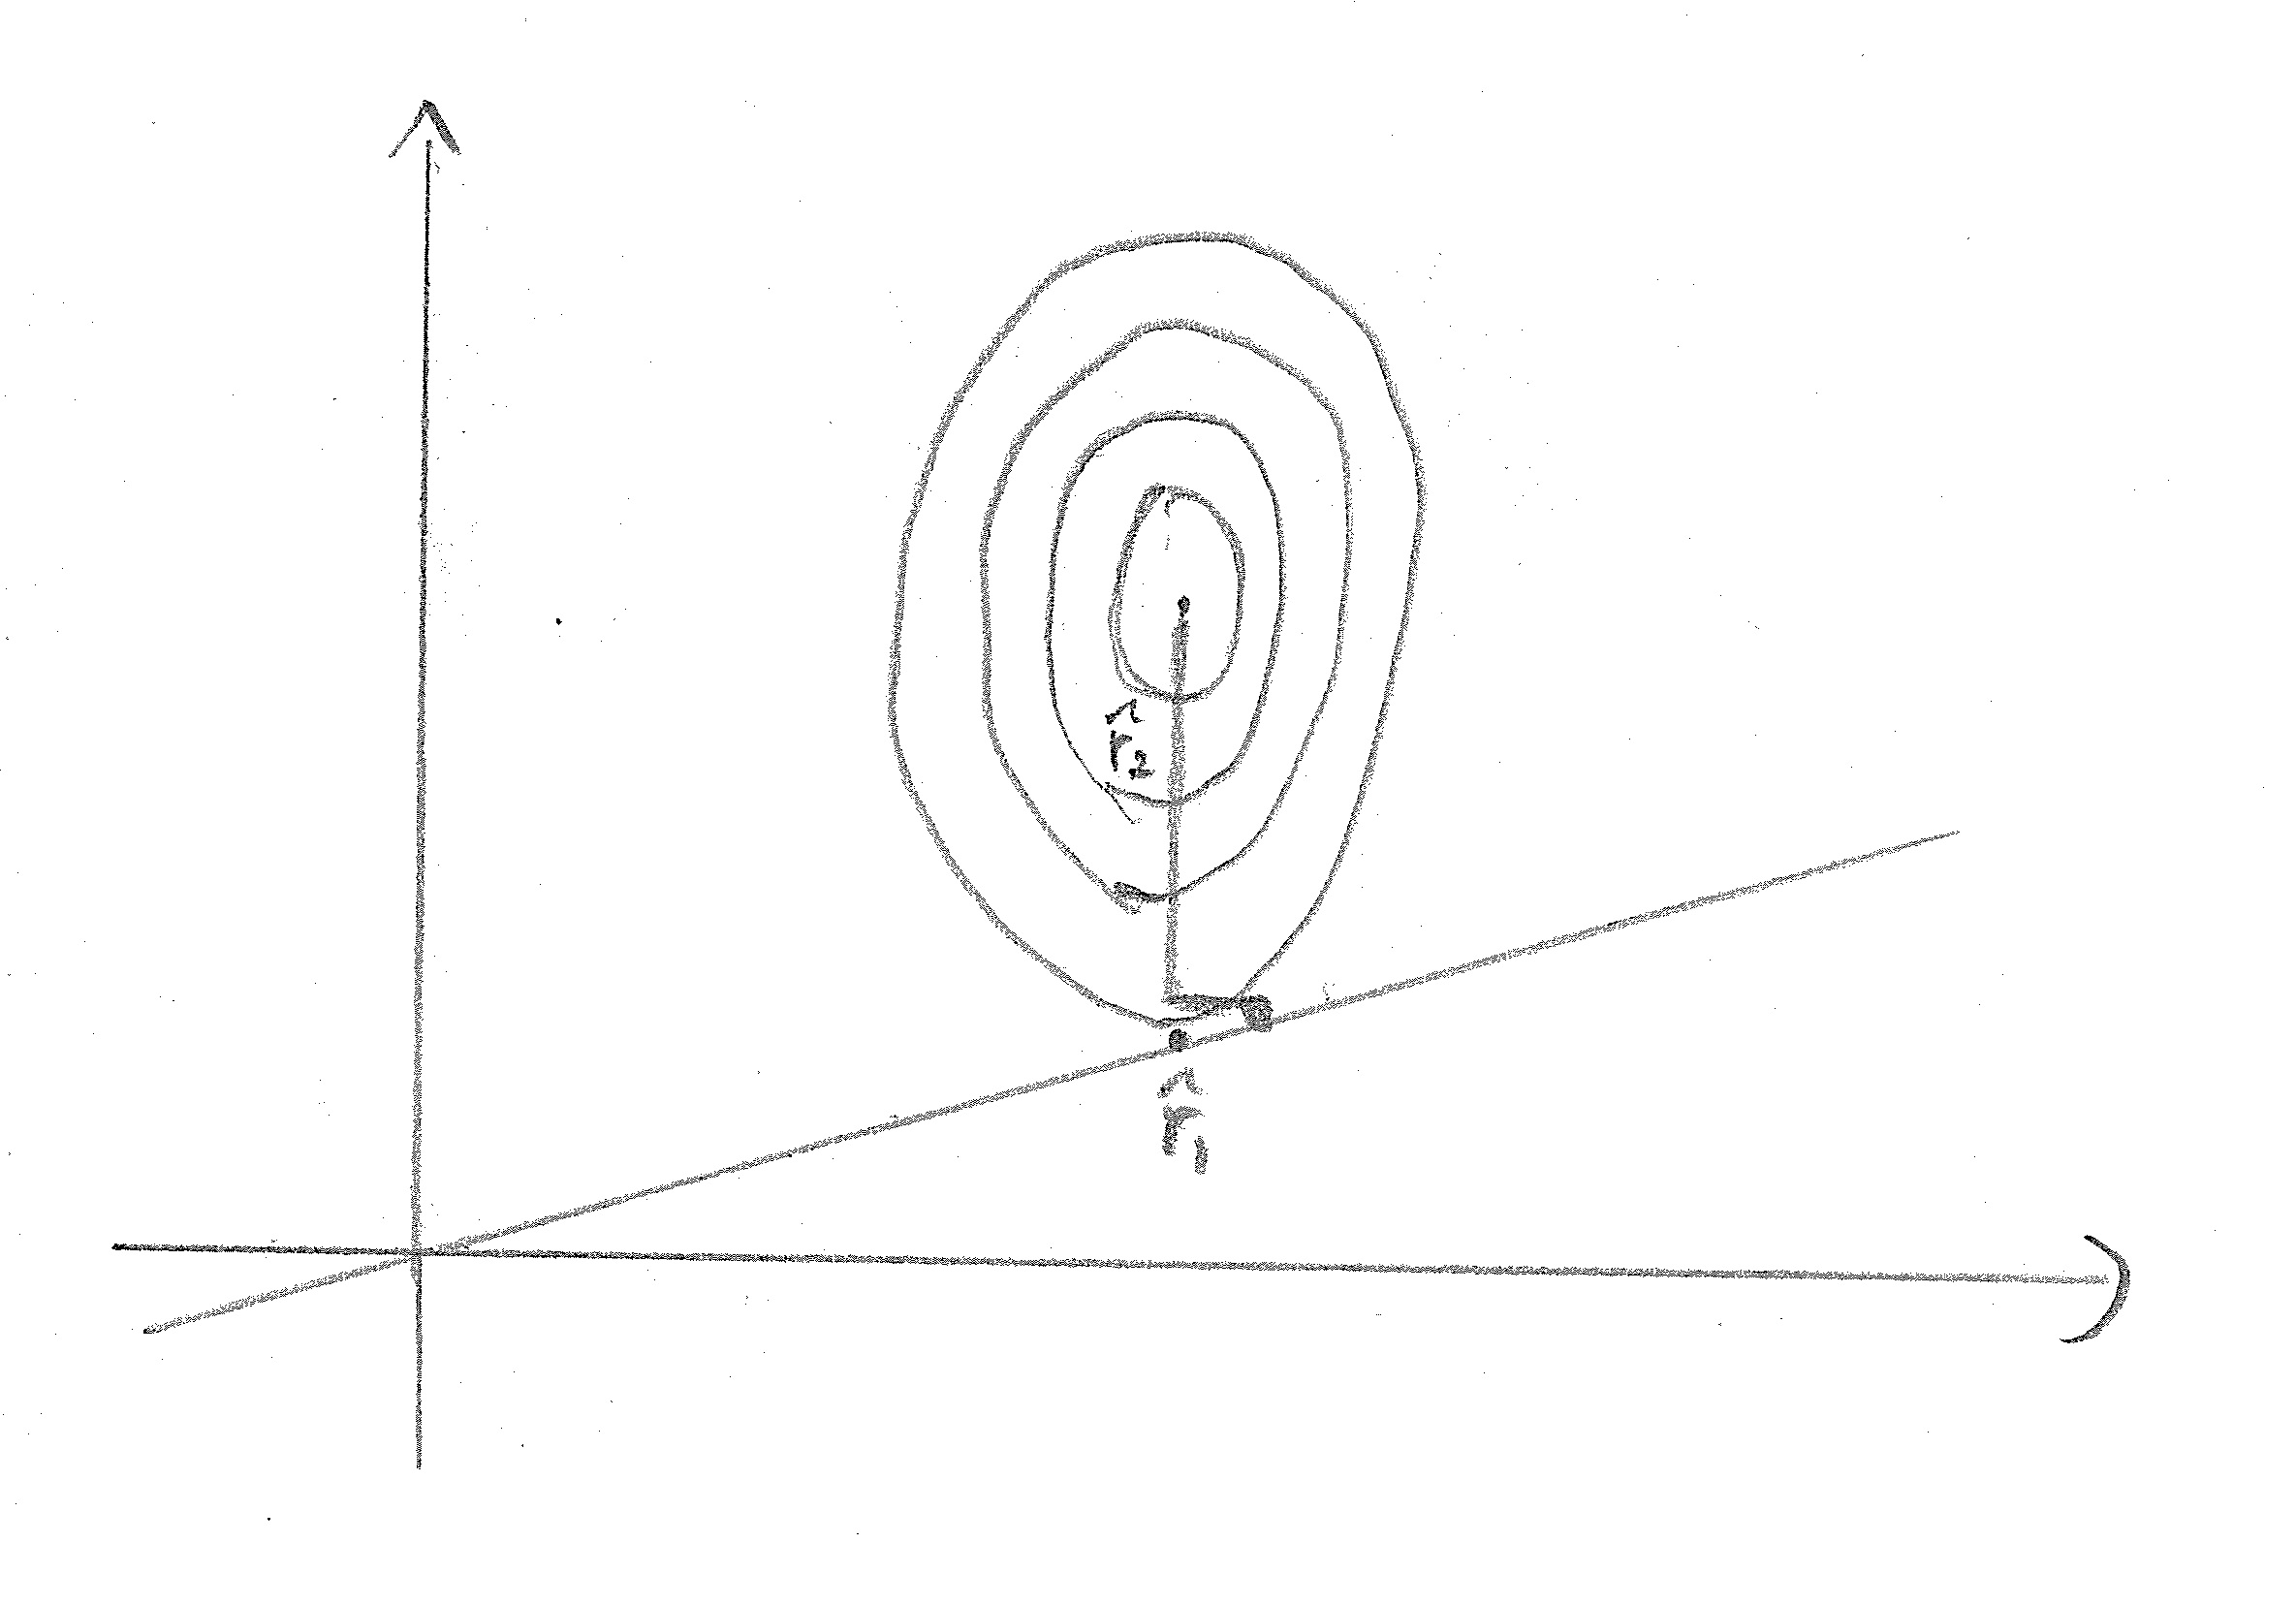
\includegraphics[width=2in,height=2in]{figures/ch06/ch06-04.jpg}
	%\caption{This is an inserted JPG graphic} 
	%\label{fig:graph} 
\end{figure}

Weighted LS with $W$ is PSD (rotation)

\begin{figure}
	\centering
	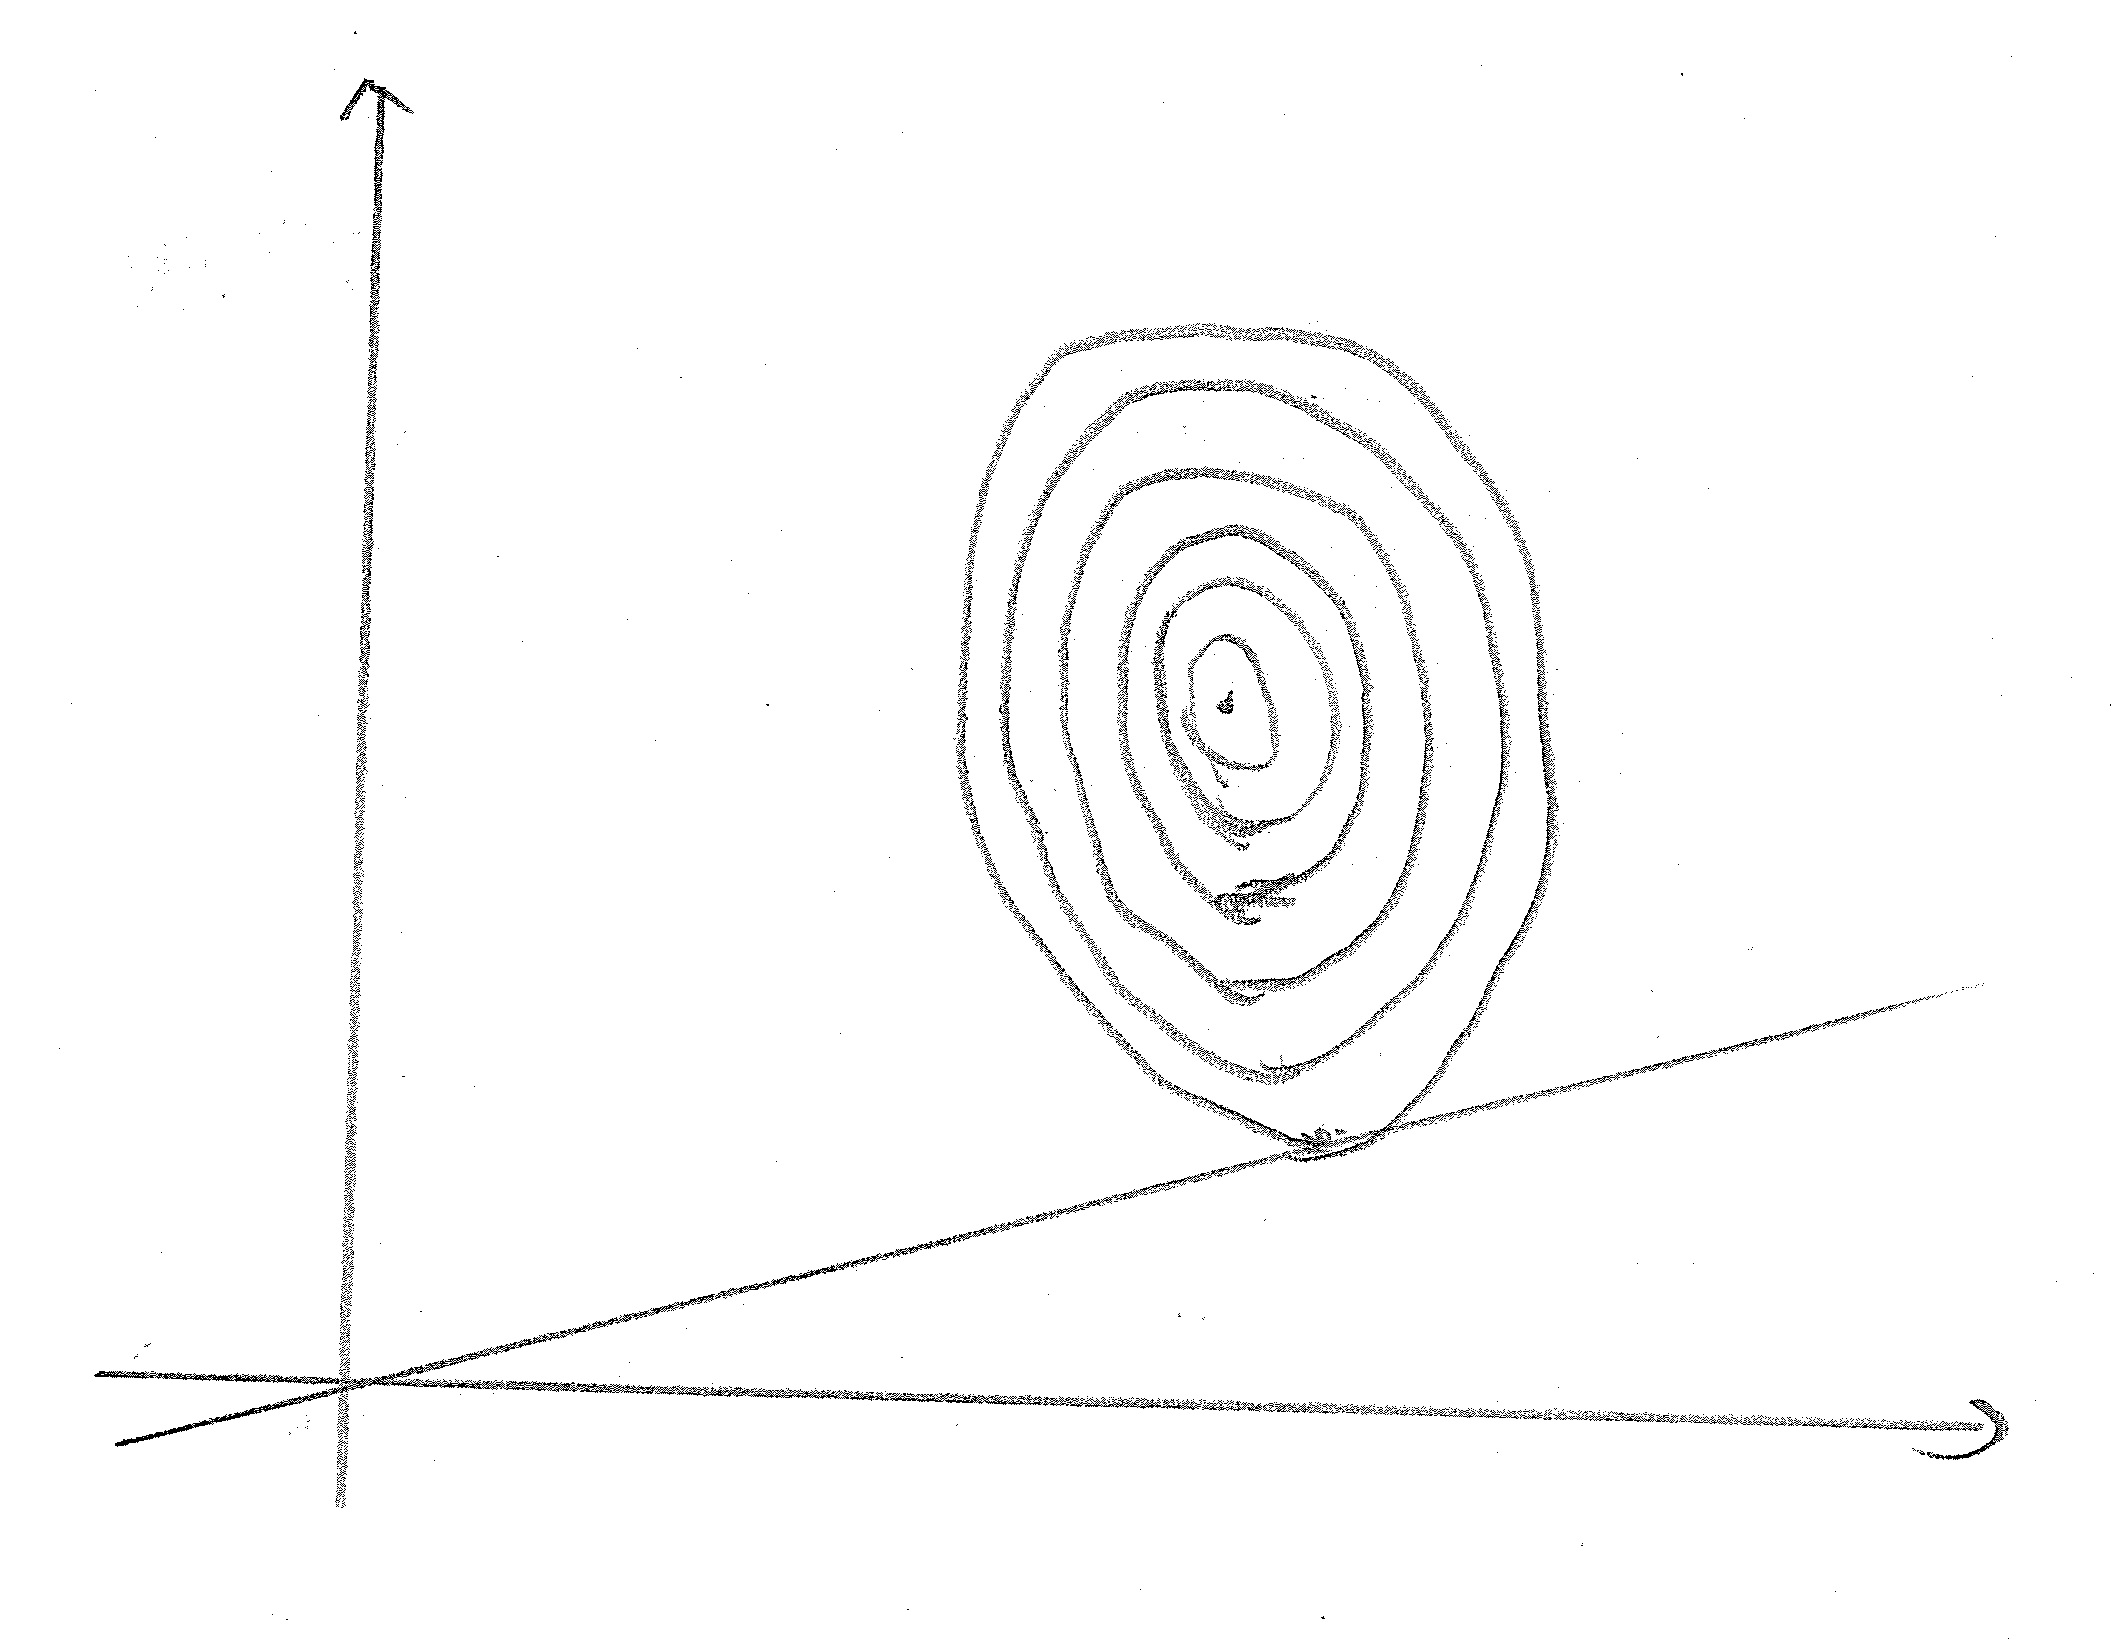
\includegraphics[width=2in,height=2in]{figures/ch06/ch06-05.jpg}
	%\caption{This is an inserted JPG graphic} 
	%\label{fig:graph} 
\end{figure}



\subsection{$L_2$- regularization least square}

In the standard least square, we do not have preference for any specific $x$ over any other, and often $x$ is a vector of resources consumed.


The $L_2$ regularized least square problem is formulated as
$$x^*=\arg_{x\in\reals_{n}} \min \Vert y-Ax\Vert ^2_2 + \gamma \Vert x\Vert ^2_2$$
where $\gamma\geq 0$ is a scalar (so if $\gamma = 0$ we retrieve the standard LS), and the term $\gamma \Vert x\Vert ^2_2$ is called the regularization or penalty term.


To solve regularized least square, we first recall a basic result regarding the $L_2$ norm, for any vectors $a$ and $b$, we have
$$\left\Vert 
\begin{bmatrix}
a\\
b
\end{bmatrix}
\right\Vert_2^2
=\Vert a \Vert_2^2 + \Vert b \Vert_2^2$$

With this useful result(can be proved easily by utilizing the definition of $L_2$ norm), we could rewrite the objective function by first define
$$
\bar{A}=
\begin{bmatrix}
A\\
\sqrt{\gamma} I_n
\end{bmatrix}
,
\bar{y}=
\begin{bmatrix}
y\\
0_n
\end{bmatrix}
$$
and therefore the objective can be written as
$$\Vert Ax - y\Vert ^2_2 + \gamma \Vert x\Vert ^2_2=\Vert \bar{A}x-\bar{y}\Vert^2_2$$

Similar with the standard least square, we can solve for $x^*$ by the following
$$x^*=(\bar{A}^{\trans} \bar{A})^{-1} \bar{A}^{\trans} \bar{y}=(A^{\trans} A+\gamma I)^{-1} A^{\trans} y$$

\subsection{Tikhonov regularization(ridge regression)}
A more general format for regularized LS allows for the introduction of weighting matrices on the
output matching residuals and on the deviation of the input term from a nominal value, resulting in the following generalize regularized problem,
$$\min_x \Vert W_1 (Ax - y)\Vert^2_2 + \Vert W_2 (x - x^{(0)})\Vert^2_2 = \min_x \Vert \bar{A}x-\bar{y}\Vert^2_2 $$
where $\bar{A} := 
\begin{bmatrix}
W_1 A\\
W_2
\end{bmatrix}
,
\bar{y} := 
\begin{bmatrix}
	W_1 y\\
	W_2 x^{(0)}
\end{bmatrix}
$
, and $W_1$ and $W_2$ are PD.

Clearly, this is a special case of our previous $L_2$ regularization, with $W_1 = I_m$, $W_2 = \sqrt{\gamma} I_n$, $x^{(0)}= 0_n$.

\subsection{Visulaize regularized least square}
Consider the regularized least square problem: 
$$\min \Vert Ax-y\Vert_2^2 +\gamma \Vert x\Vert^2_2$$

and recall our previous example, 
$$x^*= \arg_{x\in \reals^n} \min =
\left\Vert
\begin{bmatrix}
6\\
0\\
0
\end{bmatrix}
-
\begin{bmatrix}
1&0\\
1&1\\
1&2
\end{bmatrix}
\begin{bmatrix}
x_1\\
x_2
\end{bmatrix}
\right\Vert^2_2
=
\begin{bmatrix}
5\\
-3
\end{bmatrix}
$$
and we have obtained that $\Vert Ax^*-y\Vert_2^2 = 6$.


\begin{figure}
	\centering
	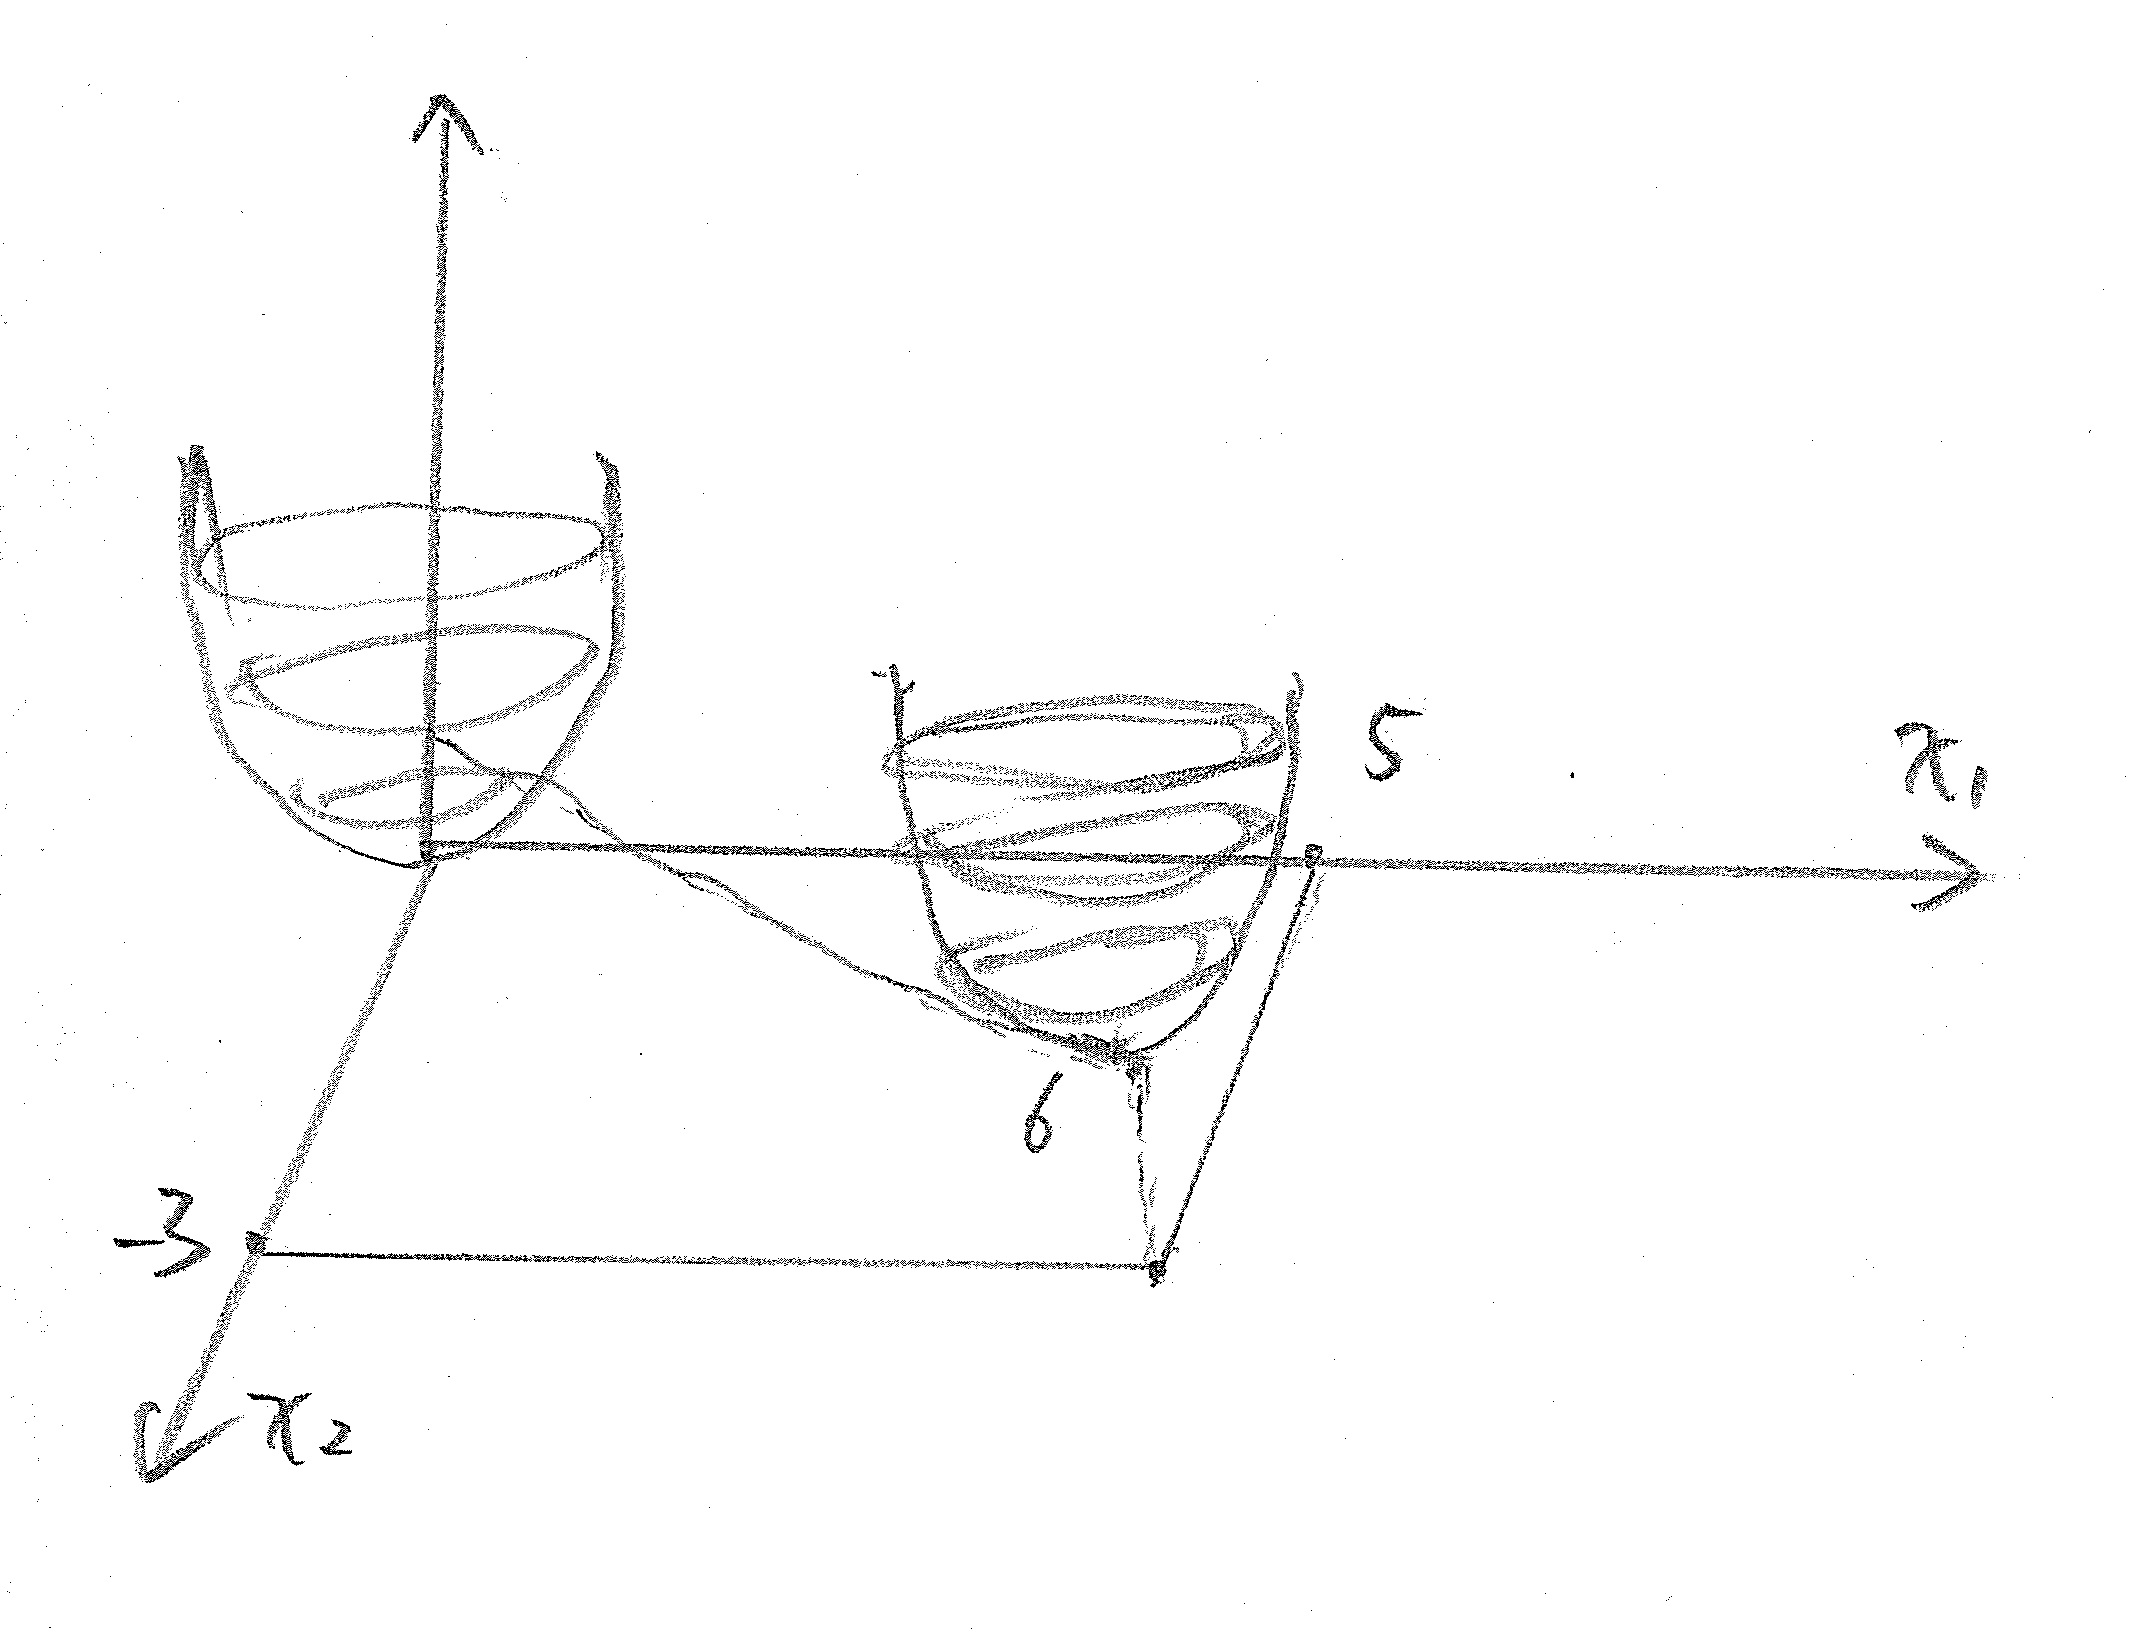
\includegraphics[width=1.8in,height=1.8in]{figures/ch06/ch06-06.jpg}
	%\caption{This is an inserted JPG graphic} 
	%\label{fig:graph} 
\end{figure}

\newpage
Draw level set for same picture
\begin{figure}
	\centering
	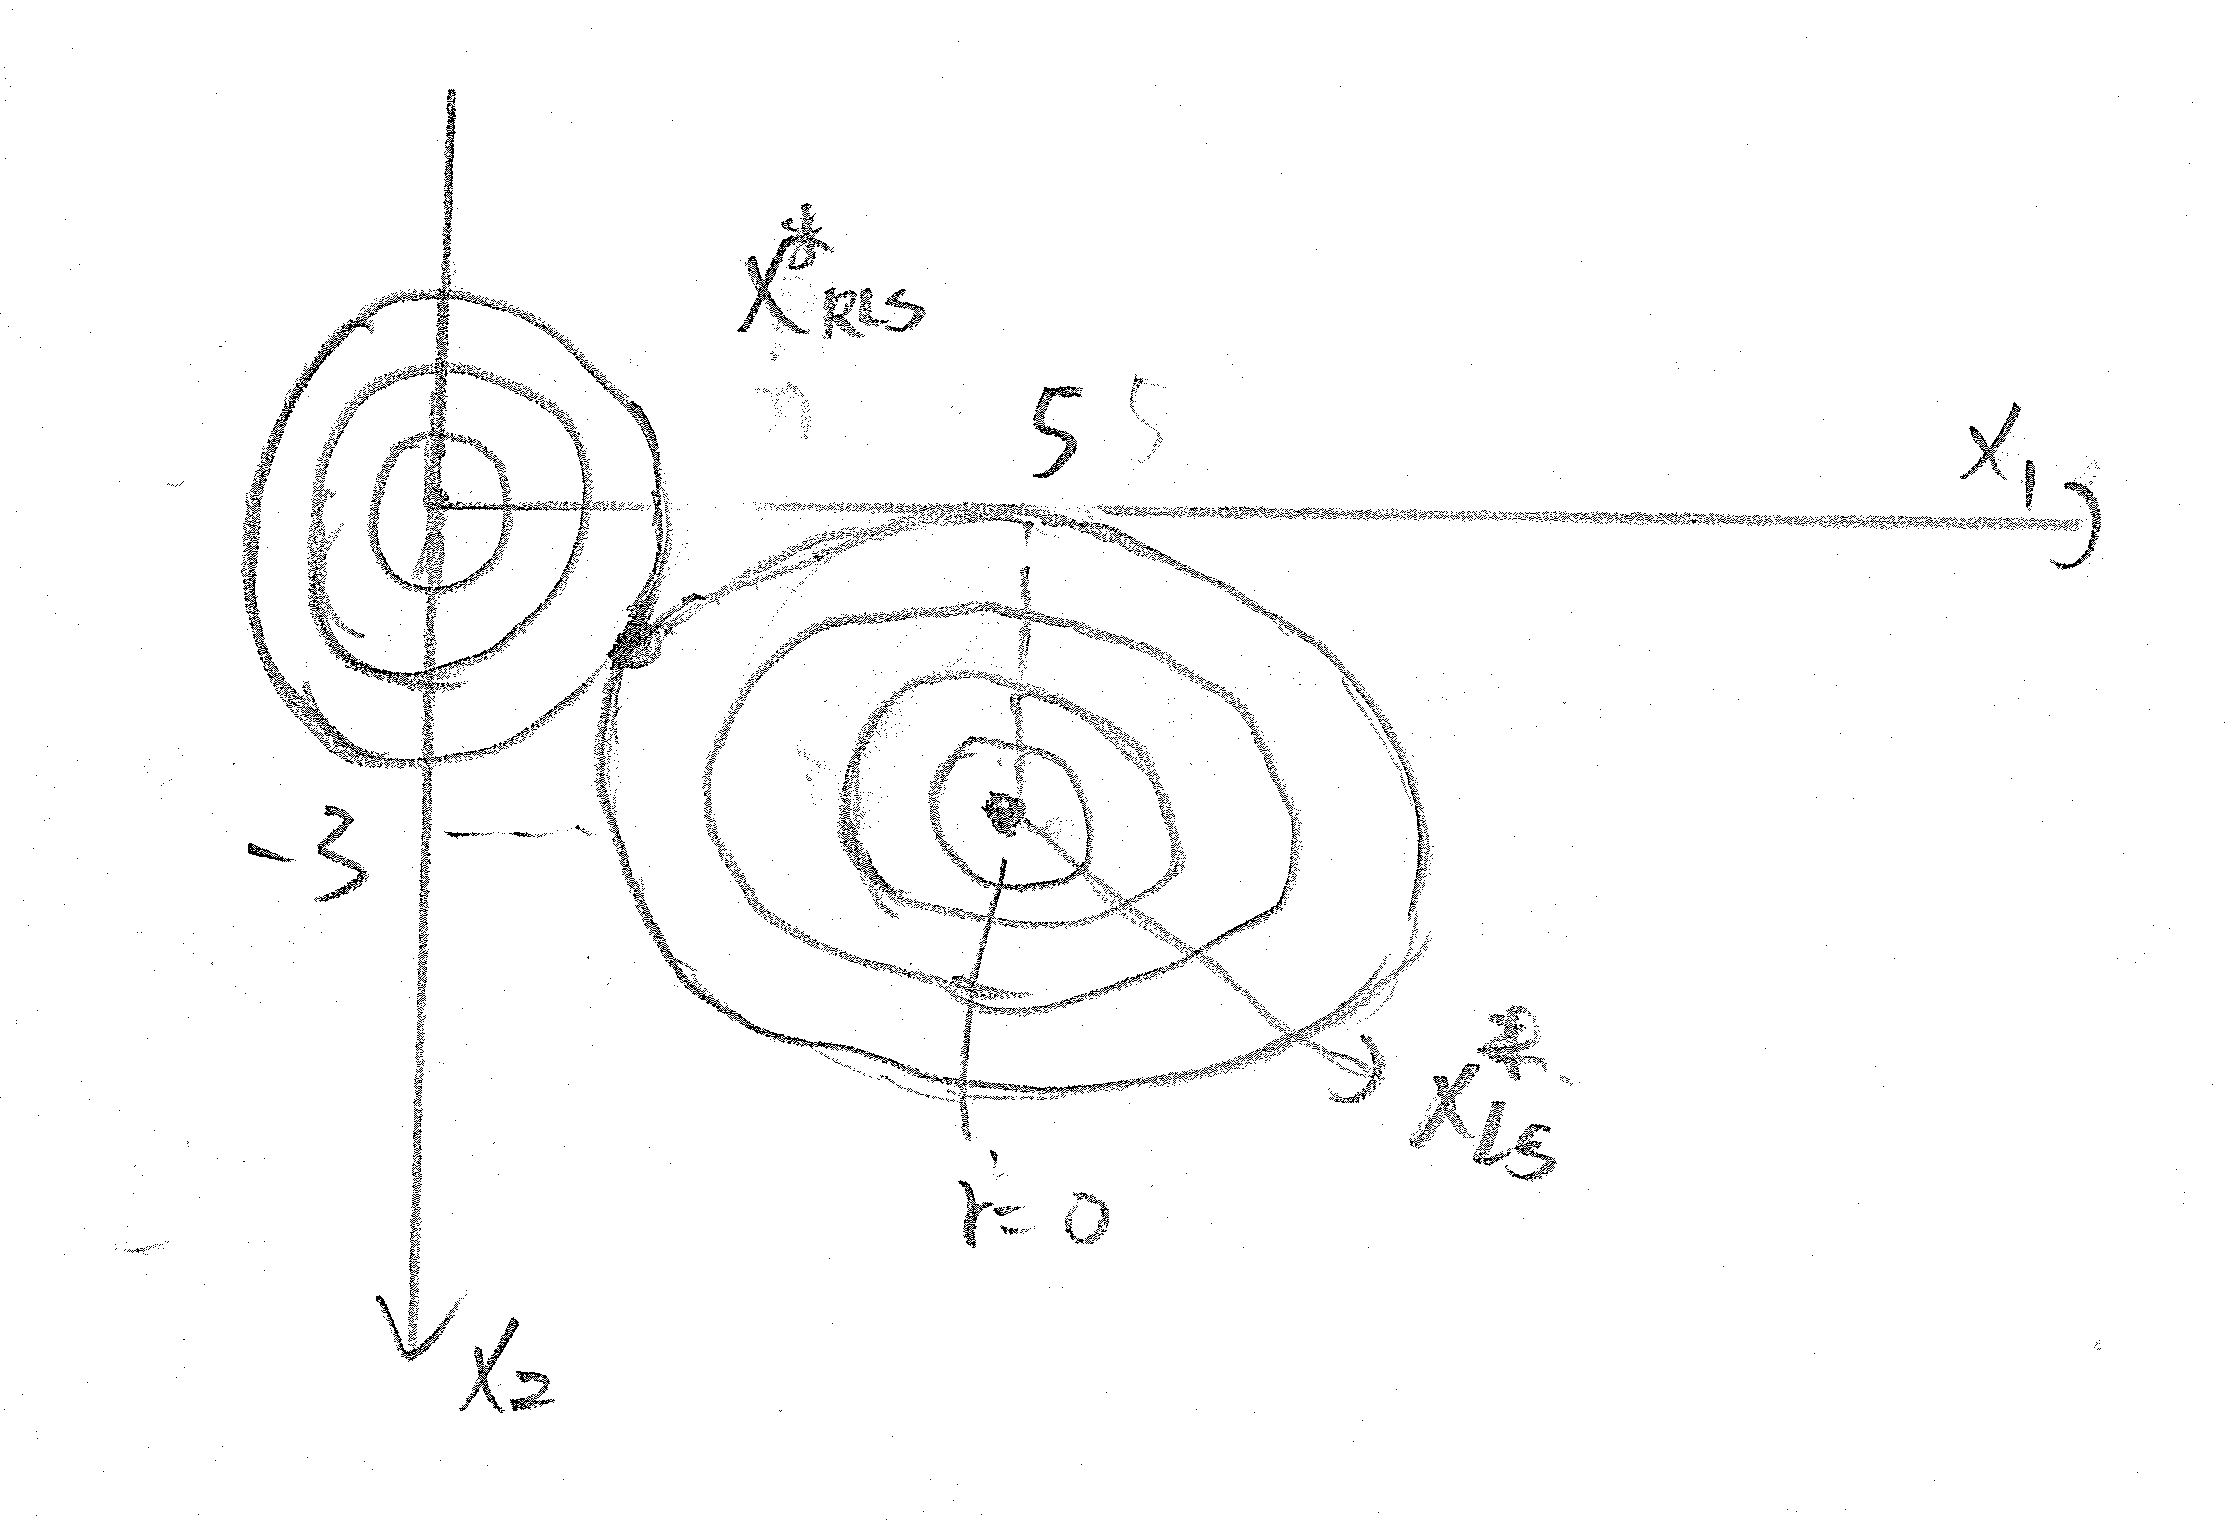
\includegraphics[width=1.8in,height=1.8in]{figures/ch06/ch06-07.jpg}
	%\caption{This is an inserted JPG graphic} 
	%\label{fig:graph} 
\end{figure}

\begin{align*}
c_1
&=\Vert Ax-y\Vert^2_2\\
&=\Vert A(x-x_{ls}^*+x_{ls}^*)-y\Vert^2_2\\
&=\Vert (Ax_{ls}^*-y)-A(x-x_{ls}^*)\Vert^2_2\\
&=\Vert (Ax_{ls}^*-y)\Vert^2_2 - \Vert A(x-x_{ls}^*)\Vert^2_2
\end{align*}

The first term on the last equality is a scalar 6(from previous example), and so we focus on the geometry of second term.
$$\Vert A(x-x_{ls}^*)\Vert^2_2= (x-x_{ls}^*)^{\trans} A^{\trans}A (x-x_{ls}^*)$$. 
Note that $A^{\trans}A$ is a PSD matrix. Understand geometry of level set of $\Vert A(x-x_{ls})\Vert^2_2$ via eigenvector of the PSD matrix $A^{\trans} A$

$$A^{\trans}A=
\begin{bmatrix}
3&3\\
3&5
\end{bmatrix}
=
\begin{bmatrix}
-0.81&0.58\\
058&0.81
\end{bmatrix}
\begin{bmatrix}
0.84&0\\
0&7.14
\end{bmatrix}
\begin{bmatrix}
-0.81&0.58\\
058&0.81
\end{bmatrix}
$$
\begin{marginfigure}
	\centering
	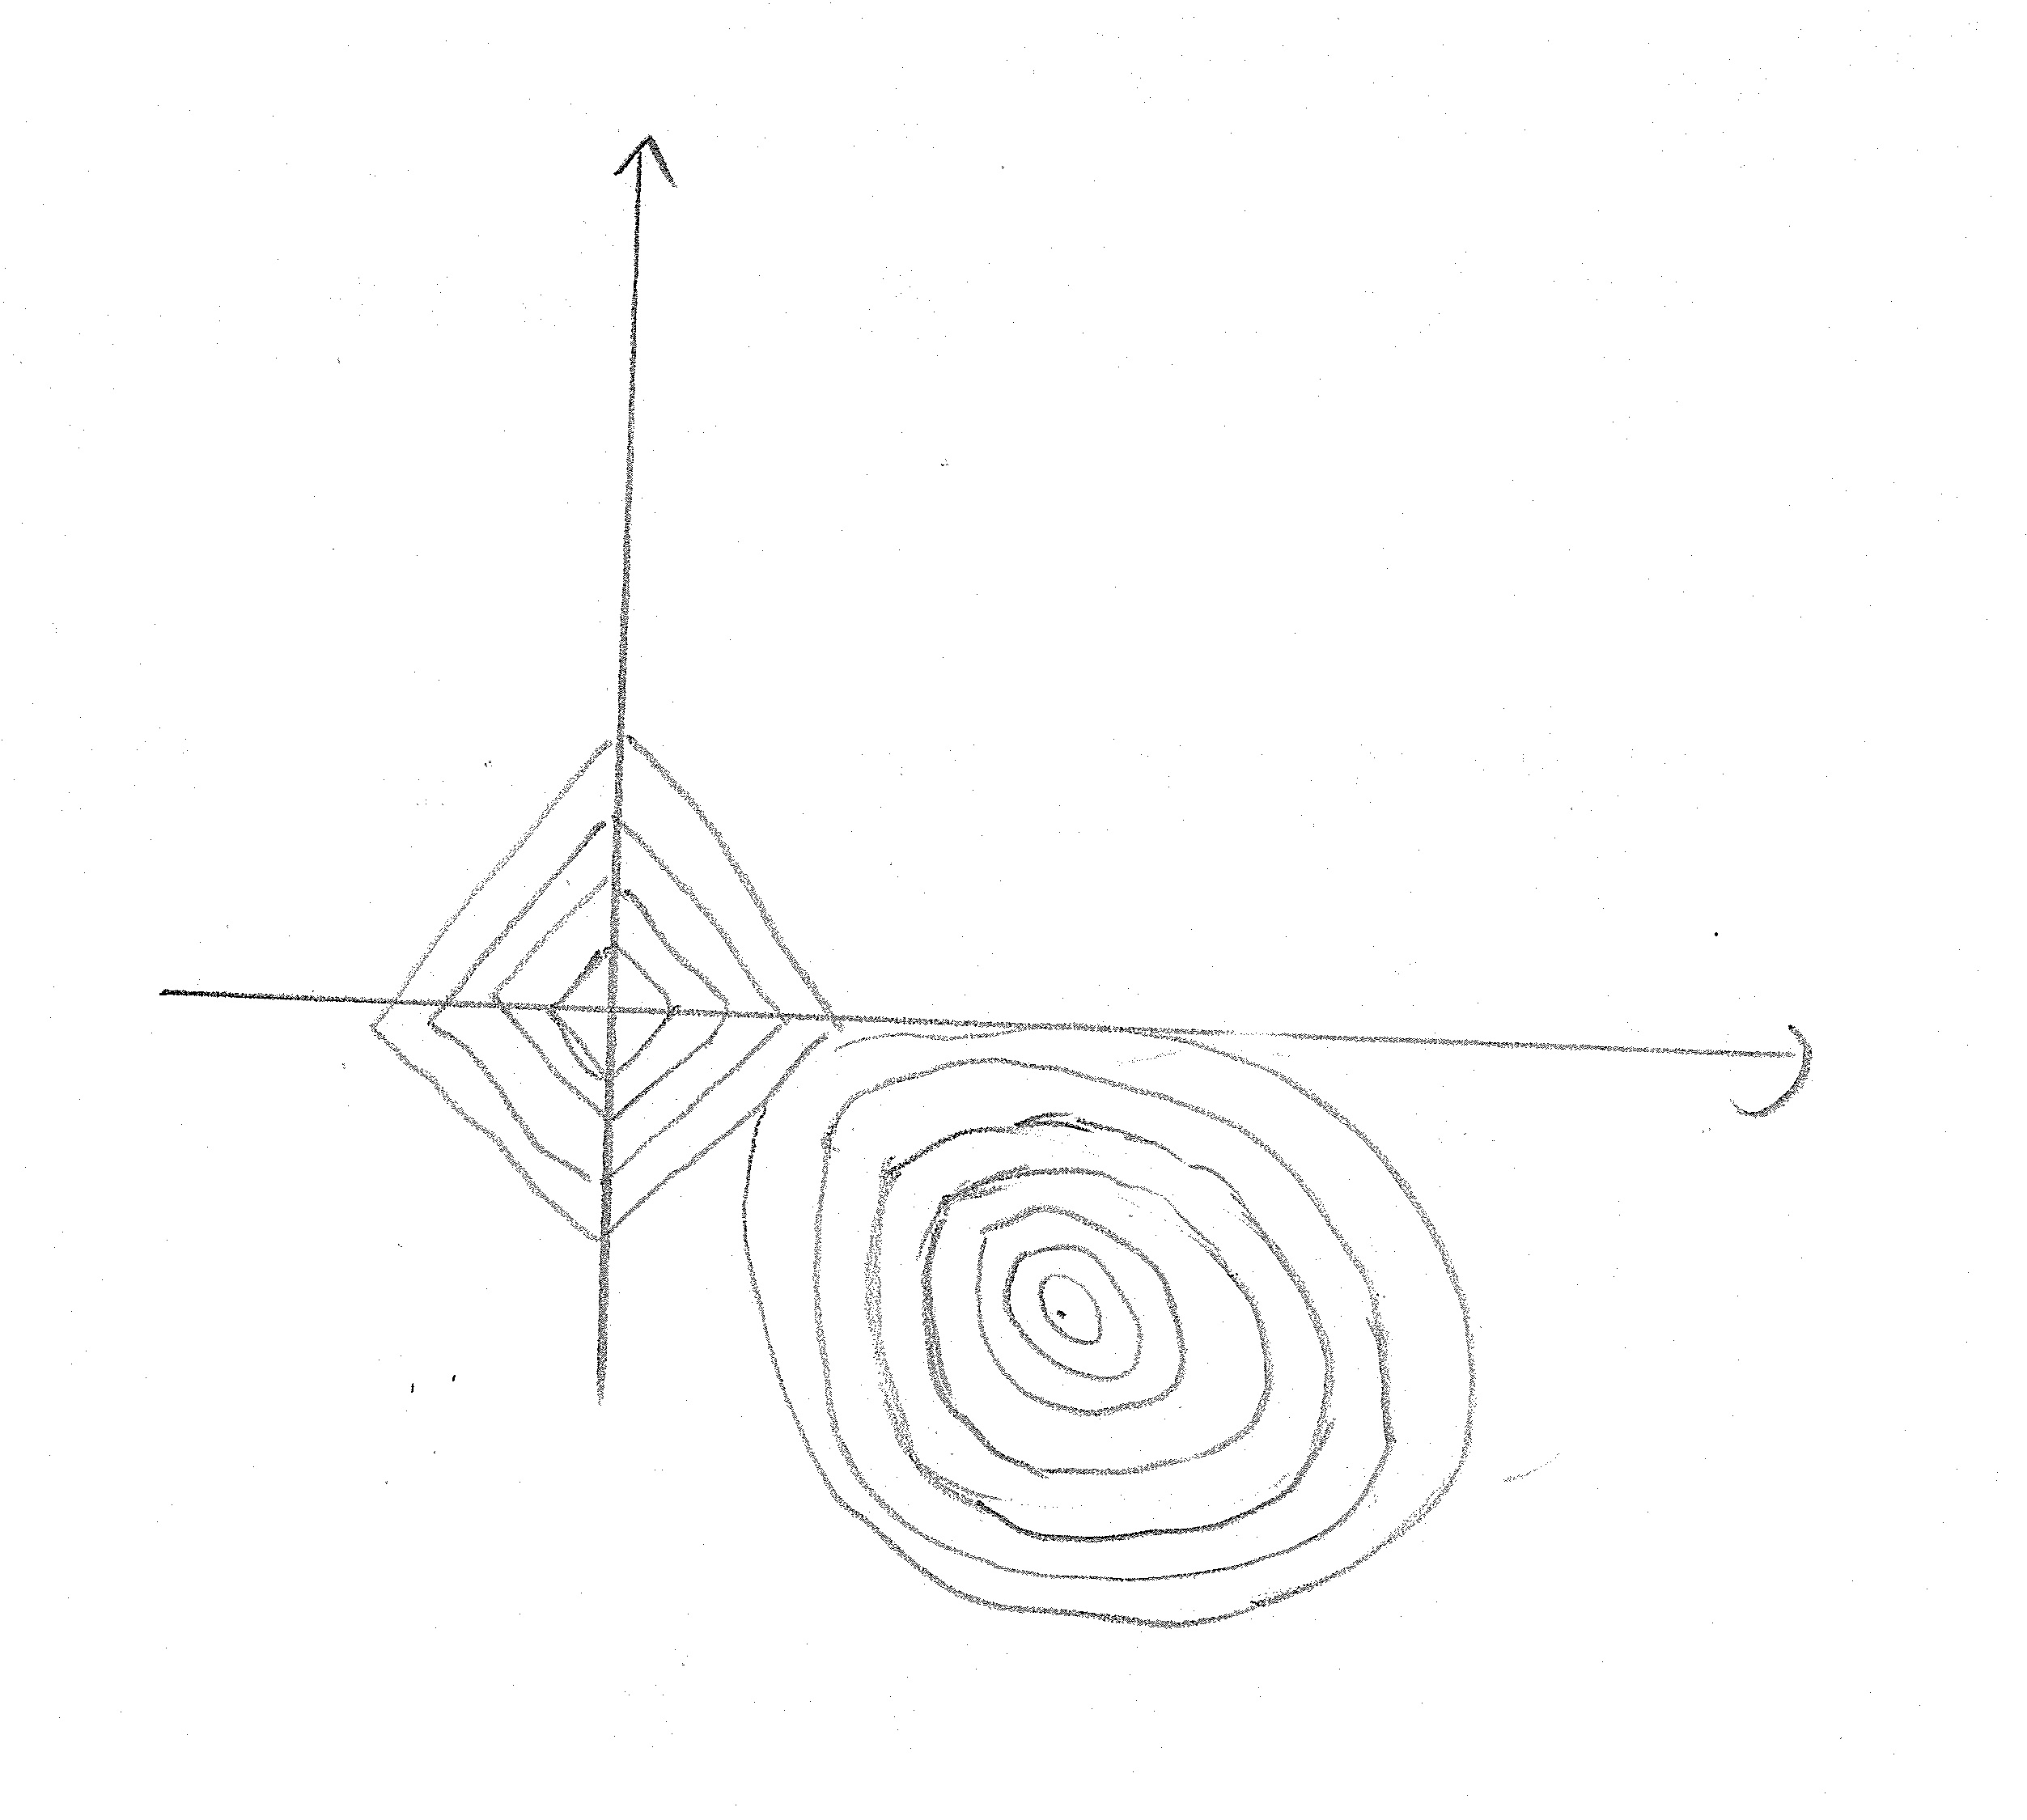
\includegraphics[width=1.8in,height=1.8in]{figures/ch06/ch06-08.jpg}
	%\caption{This is an inserted JPG graphic} 
	%\label{fig:graph} 
\end{marginfigure}


\subsection{Brief summary of Least Squares}
\begin{equation*}
x^* = \arg \min_{x\in \reals^n}\Vert y-Ax\Vert_2^2 \qquad (*)
\end{equation*}

	(1) Standard LS variant in ($*$) weights all elements of error vector equally (variant: weighted LS).
	
	(2) Standard LS measures error along standard coordinate system (change coordinate system).
	
	(3) Standard LS ignores that certain elements of $x$ may "cost" more than others (variant: regularization).

\subsection{More on "Tikhanov regularization"}
We do a simple example here, as a special case of "Tikhanov regularization, 
\begin{equation*}
x^* = \arg\min_{x\in \reals^n}\Vert y-Ax\Vert_2^2 + \gamma\Vert x\Vert_2^2
\end{equation*}

\begin{marginfigure}
	\centering
	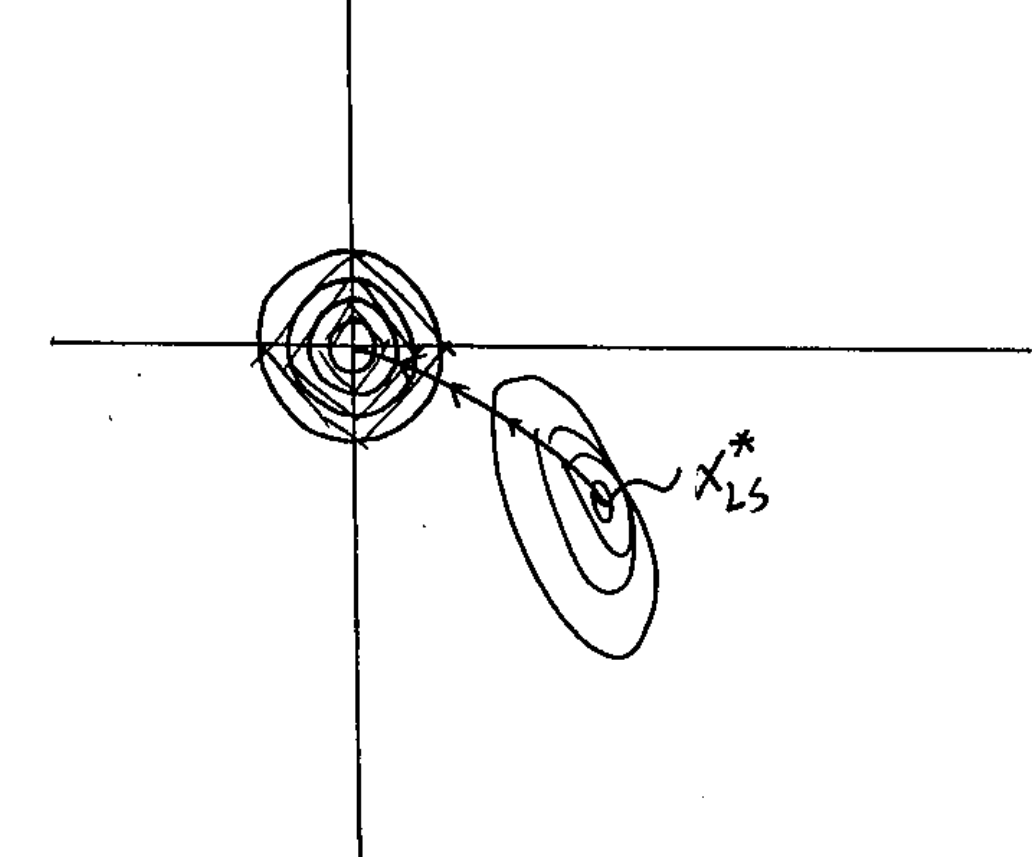
\includegraphics[width=1.8in,height=1.8in]{figures/ch06/figure4.png}
	%\caption{This is an inserted JPG graphic} 
	%\label{fig:graph} 
\end{marginfigure}

Look at the form of optimal solution 
\begin{align*}
x^* 
&= \arg\min_{x\in \reals^n}\Vert y-Ax\Vert_2^2 + \gamma\Vert x\Vert^2_2\\
&= (A^{\trans}A + \gamma I)^{-1}A^{\trans}y\\
\hat{y}^*&= Ax^* = A(A^{\trans}A + \gamma I)^{-1}A^{\trans}y\\
\end{align*}

We apply SVD to $A$,
$$A = \mathcal{U}\tilde{\Sigma}V^{\trans}$$

And utilize this to analyze $(A^{\trans}A + \gamma I)^{-1}$:
\begin{align*}
(A^{\trans}A + \gamma I)^{-1} 
&= (V\tilde{\Sigma}^{\trans}\mathcal{U}^{\trans}\mathcal{U}\tilde{\Sigma}V^{\trans} + \gamma I)^{-1}\\
&= (V
\begin{bmatrix}
\Sigma^{\trans} & 0\\
0 & 0\\
\end{bmatrix}
\begin{bmatrix}
\Sigma & 0\\
0 & 0\\
\end{bmatrix}
V^{\trans} + \gamma I)^{-1}\\
&=(V
\begin{bmatrix}
\Sigma^2 & 0\\
0  & 0
\end{bmatrix}
V^{\trans} + \gamma VV^{\trans}
)^{-1}\\
&= (V(
\begin{bmatrix}
\Sigma^2 & 0\\
0 & 0
\end{bmatrix}
+\gamma I)V^{\trans})^{-1}\\
&= V
\left[
\begin{array}{c|c}
\Sigma^2+\gamma I_r&  \\ \hline 
& \gamma I_{n-r}
\end{array}
\right]
V^{\trans}\\
&=
V
\left[
\begin{array}{c|c}
(\Sigma^2+\gamma I_r)^{-1}&  \\ \hline 
& ( \gamma I_{n-r})^{-1}
\end{array}
\right]
V^{\trans}\\
&=
V
\left[
\begin{array}{c|c}
\begin{matrix}
\frac{1}{\sigma_1^2+\gamma} & &\\
&\ddots&\\
&&\frac{1}{\sigma_r^2+\gamma}
\end{matrix}&  \\ \hline 
& \begin{matrix}
\frac{1}{\gamma} & &\\
&\ddots&\\
&&\frac{1}{\gamma}
\end{matrix}
\end{array}
\right]
V^{\trans}
\end{align*}

%\begin{matrix}
%	\frac{1}{\sigma_1^2+\gamma} & &\\
%	&...&\\
%	&&\frac{1}{\sigma_r^2+\gamma}
%\end{matrix}


%\left[
%\begin{array}{c|c}
%	\begin{matrix}
%		\frac{1}{\sigma_1^2+\gamma} & &\\
%		&...&\\
%		&&\frac{1}{\sigma_r^2+\gamma}
%	\end{matrix}&  \\ \hline 
%	& \begin{matrix}
%		\frac{1}{\gamma} & &\\
%		&...&\\
%		&&\frac{1}{\gamma}
%	\end{matrix}
%\end{array}
%\right]

\begin{align*}
y^* &= Ax^* = A(A^{\trans}A + \gamma I)^{-1}A^{\trans}y\\
&= \mathcal{U}\tilde{\Sigma}V^{\trans}\left(V
\left[
\begin{array}{c|c}
\begin{matrix}
\frac{1}{\sigma_1^2+\gamma} & &\\
&\ddots&\\
&&\frac{1}{\sigma_r^2+\gamma}
\end{matrix}&  \\ \hline 
& \begin{matrix}
\frac{1}{\gamma} & &\\
&\ddots&\\
&&\frac{1}{\gamma}
\end{matrix}
\end{array}
\right]
V^{\trans}\right)V\tilde{\Sigma}^{\trans}\mathcal{U}^{\trans}y\\
&= \mathcal{U}
\begin{bmatrix}
\Sigma & 0\\
0 & 0
\end{bmatrix}
\left[
\begin{array}{c|c}
\begin{matrix}
\frac{1}{\sigma_1^2+\gamma} & &\\
&\ddots&\\
&&\frac{1}{\sigma_r^2+\gamma}
\end{matrix}&  \\ \hline 
& \begin{matrix}
\frac{1}{\gamma} & &\\
&\ddots&\\
&&\frac{1}{\gamma}
\end{matrix}
\end{array}
\right]
\begin{bmatrix}
\Sigma^{\trans} & 0\\
0 & 0
\end{bmatrix}
\mathcal{U}^{\trans}y\\
&= \mathcal{U}
\left[
\begin{array}{c|c}
\begin{matrix}
\frac{\sigma_1^2}{\sigma_1^2+\gamma} & &\\
&\ddots&\\
&&\frac{\sigma_r^2}{\sigma_r^2+\gamma}
\end{matrix}&  \\ \hline 
& 0
\end{array}
\right]
\mathcal{U}^{\trans}y
\\
&= \mathcal{U}
\left[
\begin{array}{c|c}
\begin{matrix}
\frac{\sigma_1^2}{\sigma_1^2+\gamma} & &\\
&\ddots&\\
&&\frac{\sigma_r^2}{\sigma_r^2+\gamma}
\end{matrix}&  \\ \hline 
& 0
\end{array}
\right]
\begin{bmatrix}
\langle u^{(1)}, y\rangle\\
\langle u^{(2)}, y\rangle\\
\vdots\\
\langle u^{(m)}, y\rangle
\end{bmatrix}\\
&=\mathcal{U}
\begin{bmatrix}
\frac{\sigma_1^2}{\sigma_1^2+\gamma}\langle u^{(1)}, y\rangle\\
\vdots\\
\frac{\sigma_r^2}{\sigma_r^2+\gamma}\langle u^{(r)}, y\rangle\\
0\\
\vdots\\
0
\end{bmatrix}\\
&= \sum^r_{i=1}\frac{\sigma_i^2}{\sigma_i^2 + \gamma}\langle u^{(i)}, y\rangle u^{(i)}
\end{align*}

From the last equality,
\begin{equation*}
\sum^r_{i=1}\frac{\sigma_i^2}{\sigma_i^2 + \gamma}\langle u^{(i)}, y\rangle u^{(i)}
\end{equation*}

We should note that:
\begin{itemize}
	\item $\frac{\sigma_i^2}{\sigma_i^2 + \gamma}$: scaling is changed by regularization. If $\gamma = 0$, then  $\frac{\sigma_i^2}{\sigma_i^2 + \gamma} = 1$ and get back standard LS. If $\gamma > 0$, it's shrinkage. 
	
	\item $\langle u^{(i)}, y\rangle $: projection of data vector $y$ along that $i^{th}$ direction. 
	
	\item $u^{(i)}$: component of approximation along $i^{th}$ direction or $i^{th}$ basis element. 
\end{itemize}





%\chapter{Linear, quadratic, and geometric models}
%\label{ch.linQuadGeom}
%%% Placeholder for chapter on linear, quadratic, and geometric models

\section{Linear Programs: An Optimization Problem}
\subsection{Terminology and concepts regarding LP problem}
Consider following problem, i.e., Liner programming with equality and inequity constraints:
\begin{align*}
	\min_{x\in \reals^n}& c^{\trans}x + d\\
	s.t. \quad &Ax = b\\
	&Gx \leq h
\end{align*}

where $x\in \reals^n, c\in \reals^n, d\in \reals, A\in \reals^{q\times n}, b\in \reals^q, G\in \reals^{m\times n}, h\in \reals^m$.

Note that, the function $p(x)=c^{\trans}x + d$ is called the objective function and $x$ is called the decision variable. The goal of this problem is to find $x^*$ such that the optimal value $p^*$ of the objective function is achieved.

This formulation is the general form, and let's write it in matrix form(list of vectors), that is,

$$
A = 
\begin{bmatrix}
\alpha^{(1)^{\trans}}\\
...\\
\alpha^{(q)^{\trans}}
\end{bmatrix}
\qquad	
G = 
\begin{bmatrix}
g^{(1)^{\trans}}\\
...\\
g^{(q)^{\trans}}
\end{bmatrix}
$$

$$<\alpha^{(i)}, x> =b_i,\ i\in \left[q\right]$$
$$<G^{(i)}, x>\leq h_i,\ i\in \left[m\right]$$

Note that, there are also two other forms which are commonly used.

1. Inequality form (only contains inequity constraints)
\begin{align*}
	min \quad &c^{\trans}x+d\\
	s.t. \quad &Gx\leq h\\
\end{align*}
Given the general form, to get the inequality form, we simply break the equality
\begin{equation*}
	Ax = b \Leftrightarrow Ax\geq b, Ax\leq b
\end{equation*}
So we can get inequality form as follows:
\begin{align*}
	\min c^{\trans}x&+d\\
	\qquad s.t. \quad Gx &\leq h\\
	Ax &\leq b\\
	-Ax &\leq -b
\end{align*}

2. Standard form (only contains equality and all variables are non negative)
\begin{align*}
	\min \quad&c^{\trans}x+d\\
	s.t. \quad&Ax = b\\
	&x\geq 0
\end{align*}

Given the general form, we can also convert it into a standard form in 2 steps.

Step 1: Introducing the slack variables $s$

Given the general form,
\begin{align*}
	\min \quad&c^{\trans}x+d\\
	s.t. \quad&Gx\leq h\\
	&Ax = b
\end{align*}
We add the slack variables $s$ so that the formulation become:
\begin{align*}
	\min \quad&c^{\trans}x+d\\
	s.t. \quad&Gx + s = h\\
	&Ax = b\\
	&s\geq 0
\end{align*}
Note that the slack variables $s$ must be non negative here.


Step 2: We break the decision variable $x$ by $x= x^+ - x^-$
\begin{align*}
	\min \quad &c^{\trans}(x^{+} - x^{-})+d\\
	s.t. \quad&G(x^{+} - x^{-}) + s = h\\
	&A(x^{+} - x^{-}) = b\\
	&s\geq 0\\
	&x^{+}\geq 0\\
	&x^{-}\geq 0
\end{align*}


Concepts that are frequently used in LP (and also optimization theory):

(1) Feasible set(or feasible region): The set of points $S$ that are satisfying all the constraints, i.e.,
$$S = \{x\in\reals^{n}|Ax = b, Gx \leq h \}$$

(2) Feasible solution: The points in the feasible set $S$.

(3) Polyhedron: intersection of finite number of half-spaces, i.e.,
$$\{x\in\reals^{n}|Gx\leq h\}$$

(4) Polytope: bounded intersection of finitely many half-spaces.





\vspace{0.5cm}
Let $p^*$ be the optimal value of the given objective function under the constraints, i.e.,
\begin{align*}
	p^* = \min \quad &c^{\trans}x + d\\
	s.t.\quad &Ax = b\\
	&Gx\leq h
\end{align*}

Remarks on "optimal" value $p^*$ of program:
\begin{itemize}
	\item Lowest cost choice amongst all feasible $x$.
	
	\item Possible here is no minimal choice
	
	\item possible no feasible choice
	
	\item $p^*\in \reals$
\end{itemize}

\vspace{0.5cm}
Let $x^*$ be the optimal choice of the decision variable $x$, i.e.,
\begin{align*}
	x^* = \arg \min \quad&c^{\trans}x + d\\
	s.t.\quad &Ax = b\\
	&Gx\leq h
\end{align*}

Remarks on "optimal" solution $x^*$ of program:
\begin{itemize}
	\item Sometimes $x^*$ does not exist
	
	\item If exists, may not be unique
	
	\item $x^*\in \reals^n$
\end{itemize}




\vspace{0.5cm}
Let's consider an example:\\

During the The Second World War, the US army is considering how to make their soldiers have enough nutrients...\\

Different nutrients in different foods and daily requirement:
\begin{center}
	\begin{tabular}{|c|c|c|c|}
		\hline 
		Nutrients&Meat&Potatoes&Daily Requirement\\
		\hline  
		Carbohydrates&40&200&400\\
		\hline  
		Protein&100&20&200\\
		\hline  
		Fiber&5&40&40\\
		\hline 
	\end{tabular}
\end{center}


\vspace{0.3cm}
The price of meat and potatoes:
\begin{center}
	\begin{tabular}{|c|c|}
		\hline 
		Resources&cost/kg\\
		\hline  
		Meat &\$ 1\\
		\hline 
		Potatoes &\$ 0.25\\
		\hline 
	\end{tabular}
\end{center}

Let $x_1$ denotes meat(kg) and $x_2$ denotes potatoes(kg), and we formulate this LP as follows:

Objective function:
\begin{equation*}
	\min_{x_1, x_2} x_1 + \frac{1}{4}x_2 = 
	\min_{x_1, x_2}
	\begin{bmatrix}
		1 & \frac{1}{4}
	\end{bmatrix}
	\begin{bmatrix}
		x_1\\
		x_2
	\end{bmatrix}
\end{equation*}

Constrains:
\begin{align*}
	40x_1 + 200x_2 &\geq 400\\
	100x_1 + 20x_2 &\geq 200\\
	5x_1 + 40x_2 &\geq 40\\
	x_1 \geq 0\\
	x_2 \geq 0
\end{align*}


Rewrite it as $Gx\leq h$, that is,
\begin{equation*}
	\begin{bmatrix}
		-\frac{1}{5} & -1\\
		-\frac{1}{8} & -1\\
		-5 & -1\\
		-1 & 0\\
		0 & -1
	\end{bmatrix}
	\begin{bmatrix}
		x_1\\
		x_2
	\end{bmatrix}\leq
	\begin{bmatrix}
		-2\\
		-1\\
		-10\\
		0\\
		0
	\end{bmatrix}
\end{equation*}

\begin{figure}
	\centering
	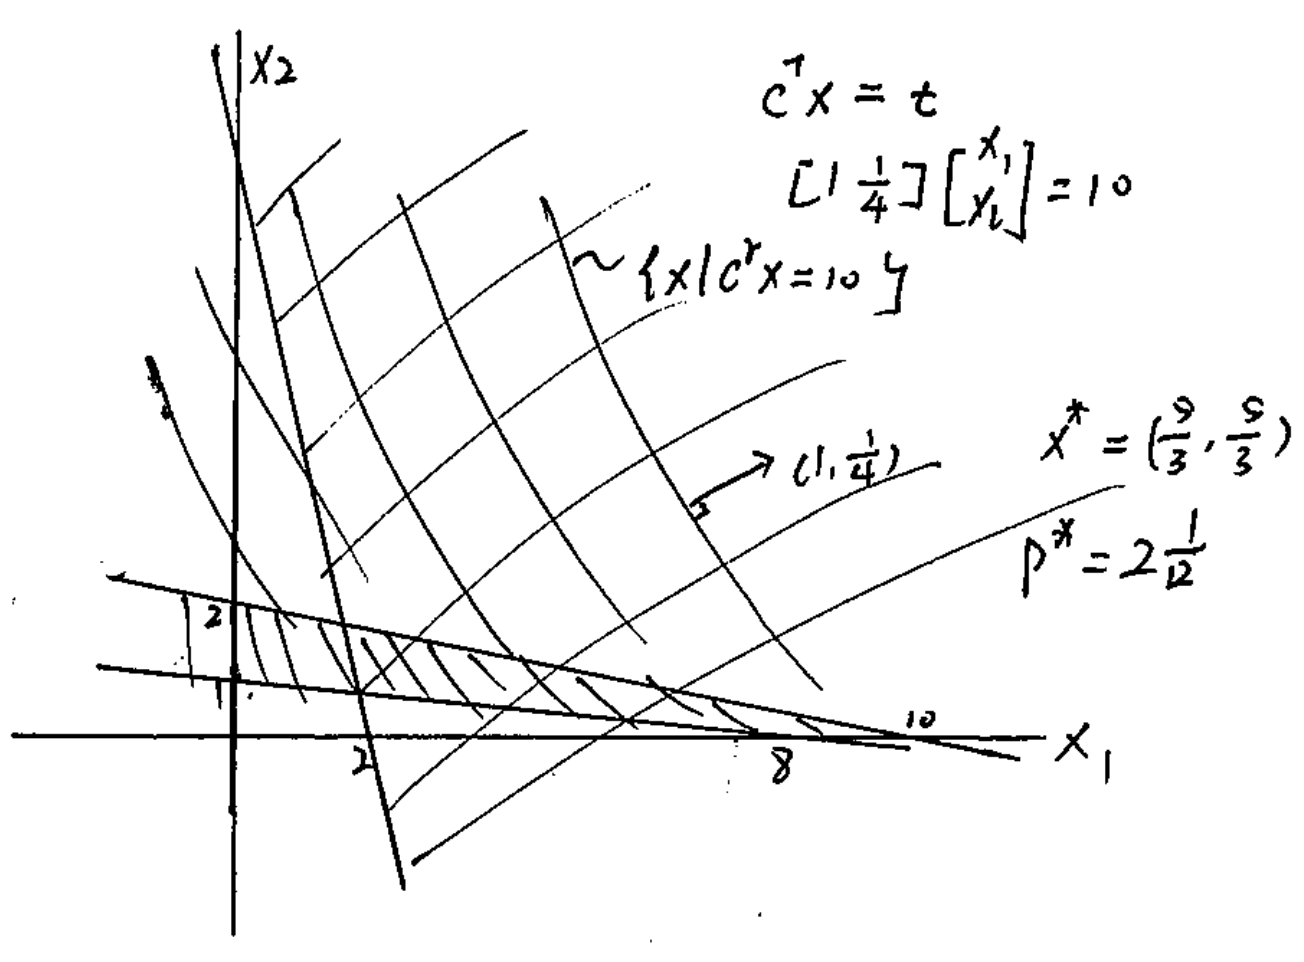
\includegraphics[width=2.1in,height=2.1in]{figures/ch06/figure5.png}
	%\caption{This is an inserted JPG graphic} 
	%\label{fig:graph} 
\end{figure}



\subsection{LP without constraints}

Consider the LP does not have constraints, so we have
\begin{align*}
	p^* &= \min c^{\trans}x+d\\
	x^* &= \arg \min_{x\in \reals^n} \quad c^{\trans}x+d
\end{align*}

\vspace{0.5cm}
Situation 1: $c = 0 \in \reals^n$
\begin{align*}
	p^* &= \min_{x\in \reals^n} \quad d=d\\
	x^* &= \arg \min_{x\in \reals^n} \quad d = \reals^n
\end{align*}

Situation 2: $c \neq 0 \in \reals^n$
\begin{align*}
	p^* &= -\infty\quad \text{by convention if no minimum}\\
	x(\alpha) &= -\alpha c \quad \alpha \geq 0\\
	c^{\trans}x + d &= c^{\trans}(-\alpha c) + d = \alpha - \alpha c^{\trans}c = \alpha - \alpha\Vert c\Vert^2_2\\
	x^* &\text{doesn't exist}
\end{align*}

Thus, for unconstrained LP we conclude that
$$
%\label{eq6}
p^*=\left\{
\begin{aligned}
d &  & \text{if } c=0 \\
-\infty &  & \text{otherwise}
\end{aligned}
\right.
%\label{eq6}
\qquad
x^*=\left\{
\begin{aligned}
\reals^n & &\text{if } c=0 \\
\text{doesn't exist} &  & \text{otherwise}
\end{aligned}
\right.
$$

Let's think about the geometry of cost function:
$$
F_0(x) =c^{\trans}x + d
$$
where $F_0(x)$ is the objective function and it turns out that it is also an affine function.

Recall that the level set for $F_0(x)$, 
\begin{align*}
	c_{F_0}(t) &=\{ x\in \reals^n | F_0(x) = c^{\trans}x + d = t \}\\
	&= \{x\in \reals^n | C^{\trans}x = (t-d) \}
\end{align*}

Obviously, the level set for $F_0(x)$ defines a hyperplane, and when $t=d$ it defines a subspace(go through the origin). Let's consider two level sets, for $t_1$ and $t_2$,

\begin{figure}
	\centering
	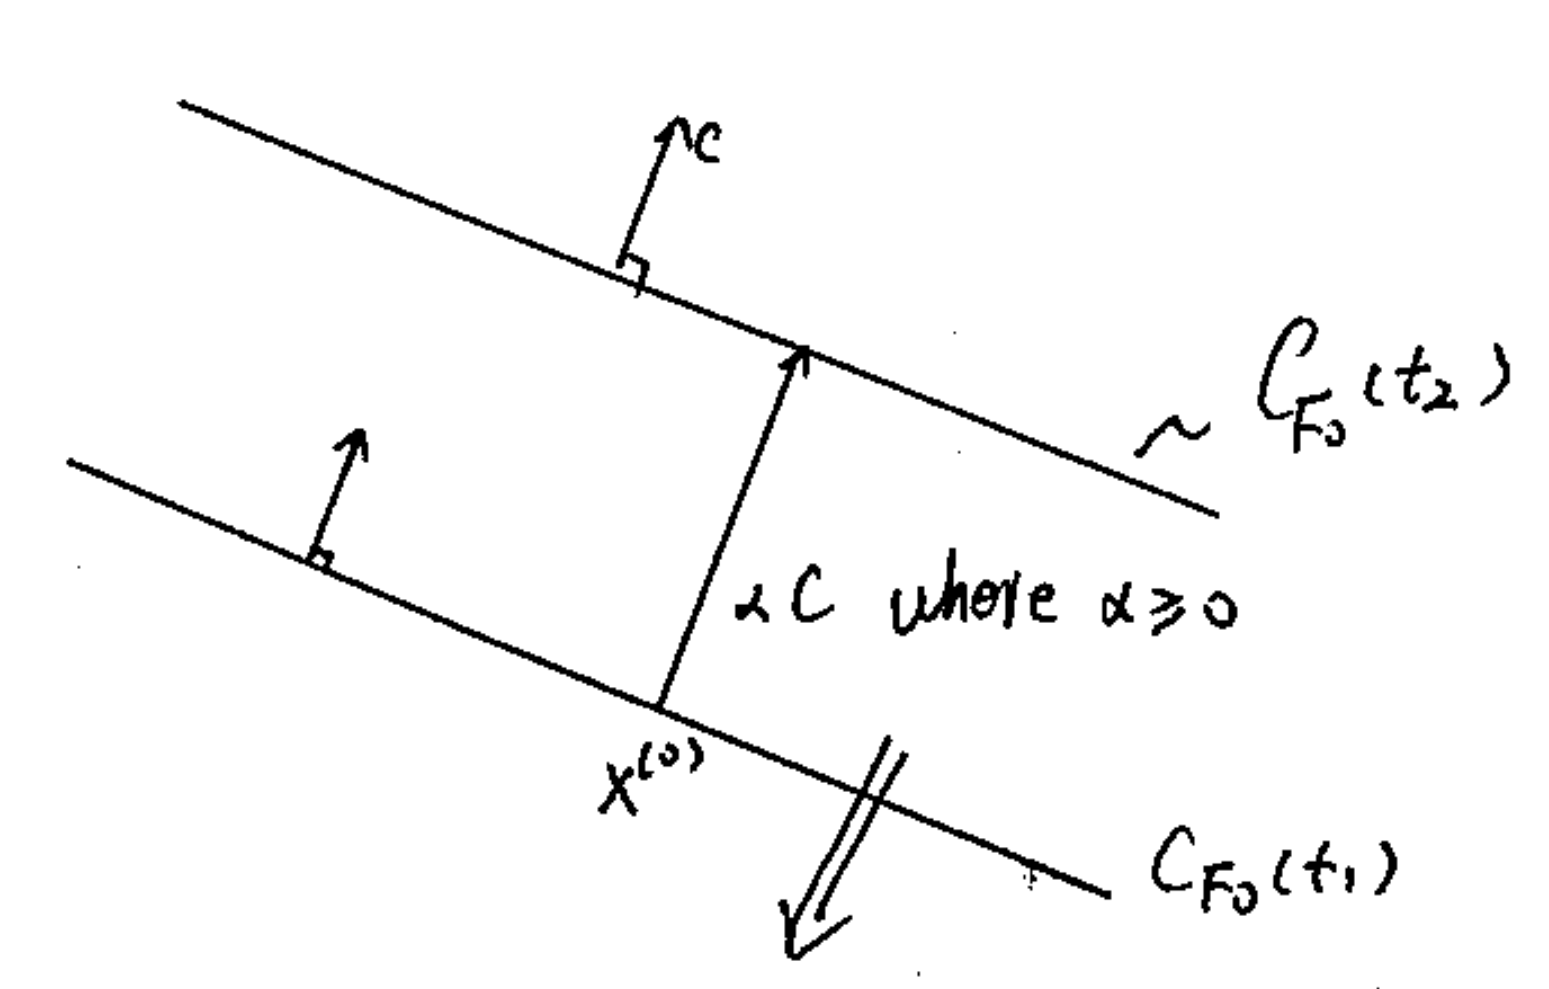
\includegraphics[width=2.1in,height=2.1in]{figures/ch07/figure1012_1.png}
	%\caption{This is an inserted JPG graphic} 
	%\label{fig:graph} 
\end{figure}

Note that $c$ is the normal vector to $x$. Let's find the relationship between $t_1$ and $t_2$:

Approach (1)
\begin{align*}
	t_2 &= c^{\trans}(x^{(0)}+\alpha c) + d\\
	t_1 &= c^{\trans}x^{(0)} + d\\
	t_2 - t_1 &= [c^{\trans}x^{(0)} + d + \alpha \Vert c\Vert ^2] - c^{\trans}x^{(0)} = \alpha \Vert c \Vert^2
\end{align*}
So apparently $t_2>t_1$.

Approach (2)
\begin{equation*}
	\nabla F_0(x) =
	\begin{bmatrix}
		\frac{\sigma}{\sigma x_1}(c^{\trans}x+d)\\
		\vdots\\
		\frac{\sigma}{\sigma x_n}(c^{\trans}x+d)
	\end{bmatrix} = 
	\begin{bmatrix}
		c_1\\
		c_2\\
		\vdots\\
		c_n
	\end{bmatrix} = c
\end{equation*}

The gradient points out that the direction of $c$ is the direction of increase in $F_0(x)$. In fact, we could show that the direction of the gradient evaluated at a certain point, is the direction that the value of function increases more rapidly(remind yourself what you have learned in Calculus).

Hence, to minimize the objective function, we go in opposite direction of the gradient, that is, we should go as far as possible along the direction of $-c$ (unless $c=0$).


\vspace{0.5cm}
Now, let's turn back to LP with following constraints as we specified before:
\begin{align*}
	Ax &= b\\
	Gx &\leq h
\end{align*}

Interesting results and interpretation for these two kind of constraints:

(1) $Ax=b$ (Equality constraints): force $x^*$ into an affine set
$$\{x\in \reals^n|Ax = b \} =  \cap^q_{i=1}\{x\in \reals^n|<\alpha^{(i)}, x> = b_i \}$$

(2) $Gx\leq h$ (Inequality constraints): force $x^*$ to be in an intersection of half-spaces
$$\{x\in \reals^n|Gx \leq h \} =  \cap^q_{i=1}\{x\in \reals^n| <g^{(i)}, x> \leq h_i \}$$

(3) The feasible set: intersection of half-spaces and hyperplanes
$$
S = \left(\cap^q_{i=1}\{x\in \reals^n | <\alpha^{(i)}, x> = b_i \}\right) \cap \left(\cap^m_{i=1}\{x\in \reals^n | <g^{(i)}, x> \leq h_i \}\right)
$$


A few remarks:
\begin{itemize}
	\item Concepts of polyhedron and polytope.
	
	\item Ax = b $\rightarrow$ $Ax \leq b$, $Ax \geq b$
\end{itemize}



\begin{example}
	\begin{align*}A &= 
		\begin{bmatrix}
			1 & 1
		\end{bmatrix}
		b = 
		\begin{bmatrix}
			2
		\end{bmatrix}\\
		G &= 
		\begin{bmatrix}
			-1 & 0\\
			0 & -1
		\end{bmatrix}
		h = 
		\begin{bmatrix}
			0\\
			0
		\end{bmatrix}\\
		Ax &= b \rightarrow x_1 + x_2 = 2\\
		Gx &\leq h \rightarrow x_1 \geq 0, x_2\geq 0
	\end{align*}
	
	
	\begin{figure}
		\centering
		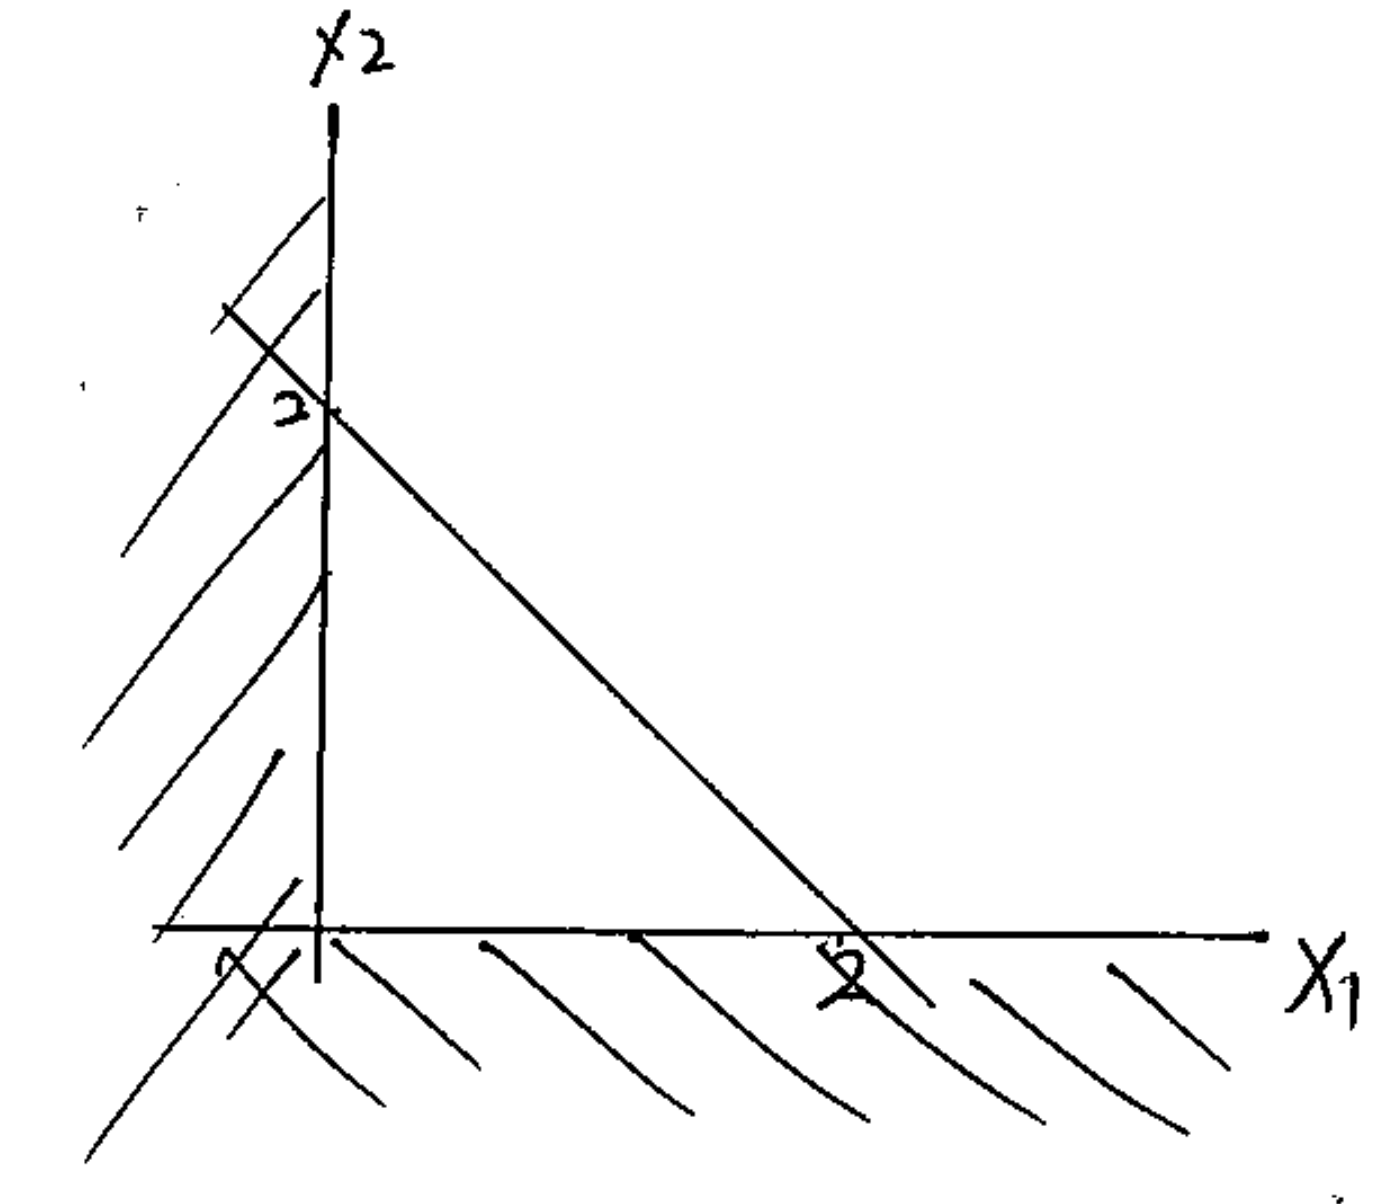
\includegraphics[width=2.1in,height=2.1in]{figures/ch07/figure1012_2.png}
		%\caption{This is an inserted JPG graphic} 
		%\label{fig:graph} 
	\end{figure}
\end{example}








\begin{example}
	Generally, equality constraints move you from a higher dimensional geometry in $\reals^n$ to a slice, which is a lower dimensional geometry. See the following example of losing 1 dimension per linearly independent constraint:
	
	
	\begin{align*}
		A =
		\begin{bmatrix}
			1&1&1
		\end{bmatrix}
	\end{align*}
	\begin{equation*}
		B= 
		\begin{bmatrix}
			1\\
		\end{bmatrix}
	\end{equation*}
	
	\begin{figure}
		\centering
		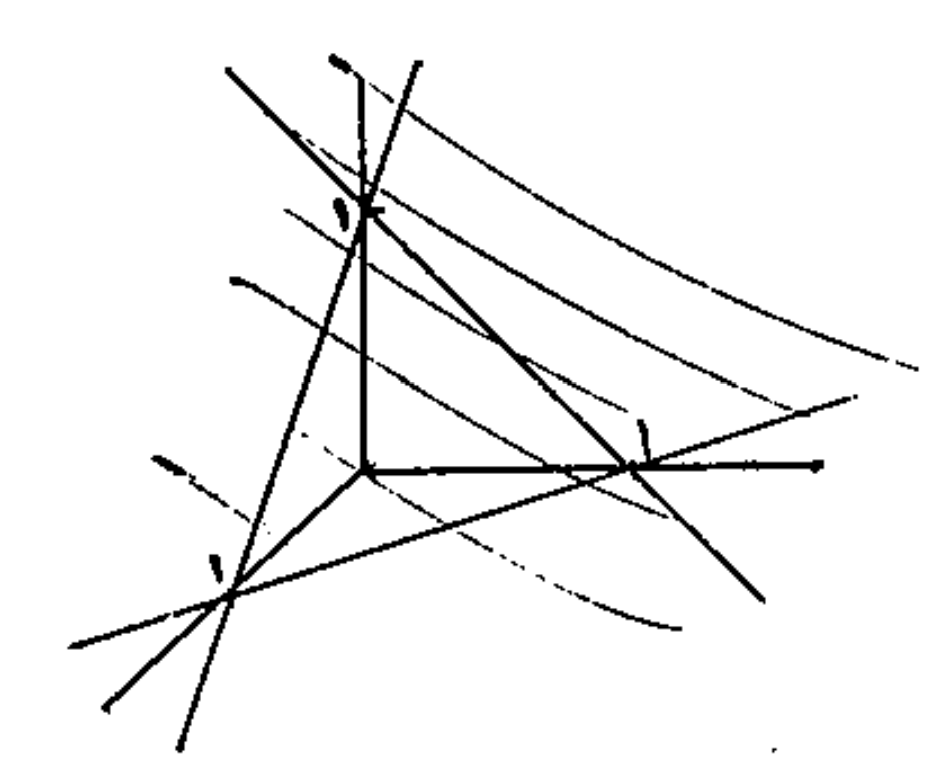
\includegraphics[width=2.1in,height=2.1in]{figures/ch07/figure1012_3.png}
		%\caption{This is an inserted JPG graphic} 
		%\label{fig:graph} 
	\end{figure}
\end{example}

\begin{example}
	In some cases, there may be no intersection between hyperplane:
	
	\begin{equation*}
		\begin{bmatrix}
			1&1\\
			1&1
		\end{bmatrix}
		\begin{bmatrix}
			x_1\\
			x_2
		\end{bmatrix}=
		\begin{bmatrix}
			1\\
			2
		\end{bmatrix}
	\end{equation*}
	
	\begin{figure}
		\centering
		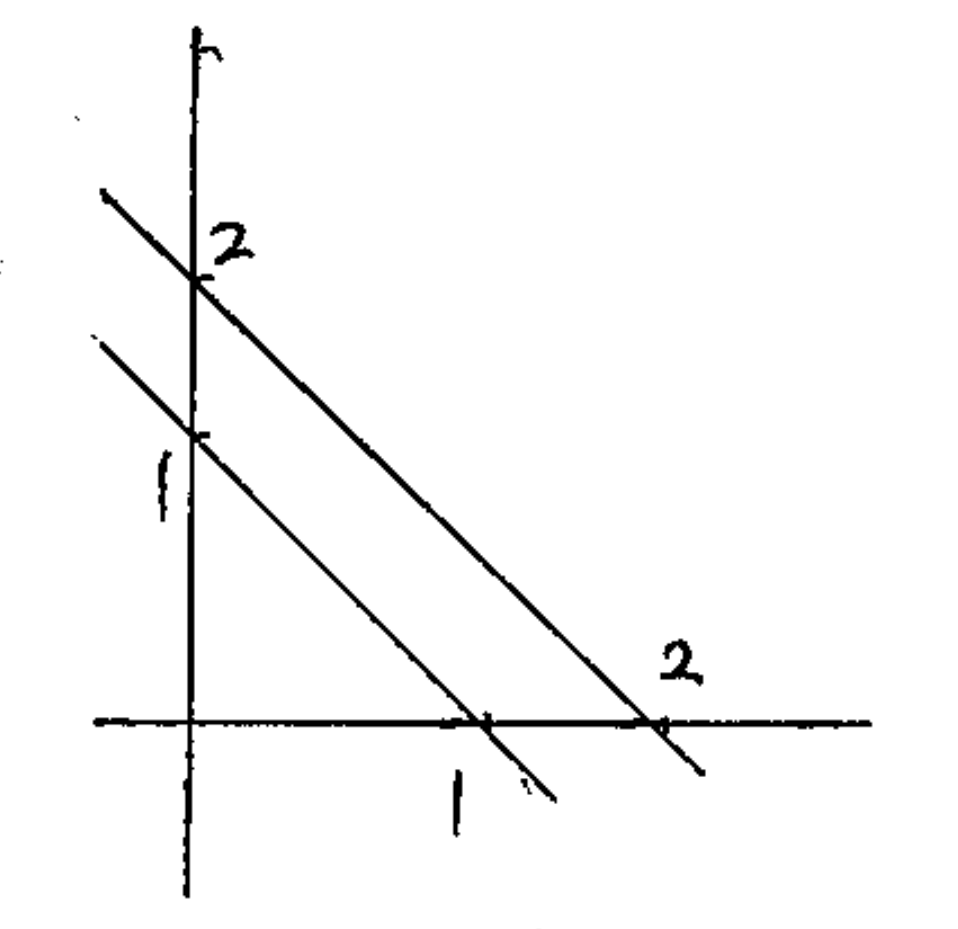
\includegraphics[width=2.1in,height=2.1in]{figures/ch07/figure1012_4.png}
		%\caption{This is an inserted JPG graphic} 
		%\label{fig:graph} 
	\end{figure}
	So the  feasible set is empty, $S = \emptyset$.
	
	\vspace{0.3cm}
	This situation may also happen with inequalities constraints:
	\begin{align*}
		\begin{bmatrix}
			-1&0\\
			1&0
		\end{bmatrix}
		\begin{bmatrix}
			x_1\\
			x_2
		\end{bmatrix}&\leq
		\begin{bmatrix}
			0\\
			-1
		\end{bmatrix}\\
		S &= \emptyset
	\end{align*}
	
\end{example}



\begin{example}
	Generally, to facilitate sketch will often just sketch inequity constraints:
	
	\begin{align*}
		\begin{bmatrix}
			-1 & 0\\
			0 & -1\\
			\frac{1}{2} & -1\\
			1 & 1
		\end{bmatrix}
		\begin{bmatrix}
			x_1\\
			x_2
		\end{bmatrix}
		&\leq 
		\begin{bmatrix}
			0\\
			0\\
			1\\
			3
		\end{bmatrix}\\
	\end{align*}
	
	So we have
	$$x_1 \geq 0$$
	$$x_2 \geq 0$$
	$$x_2 \geq -1 + \frac{1}{2}x_1$$
	$$x_2 \leq 3 - x_1$$
	
	Sketch the feasible set:
	
	\begin{figure}
		\centering
		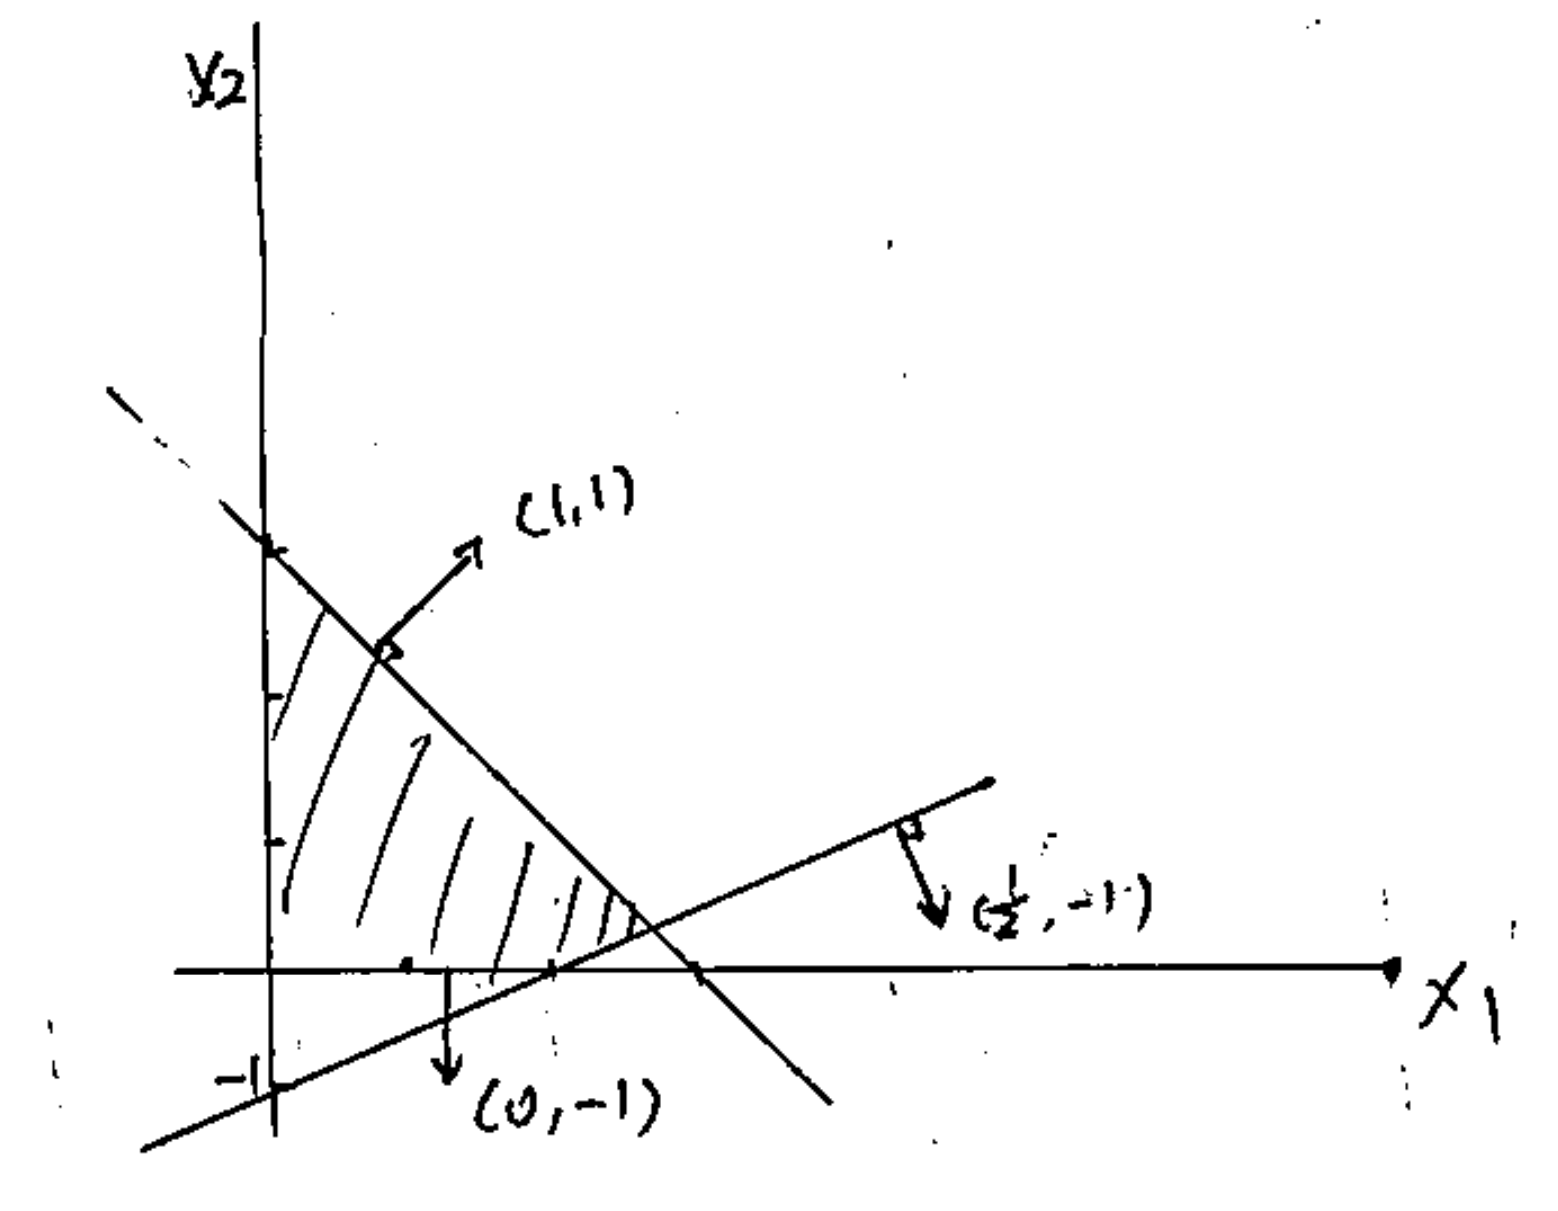
\includegraphics[width=2.1in,height=2.1in]{figures/ch07/figure1012_5.png}
		%\caption{This is an inserted JPG graphic} 
		%\label{fig:graph} 
	\end{figure}
\end{example}

The rows of matrix $G$ are the normal directions of the hyperplanes that define the half-spaces, and the normal directions point outward from the feasible set.


\begin{example}
	Let's combine all these things together, liner objective function, linear equality constraints and linear inequity constraints.
	
	\begin{figure}
		\centering
		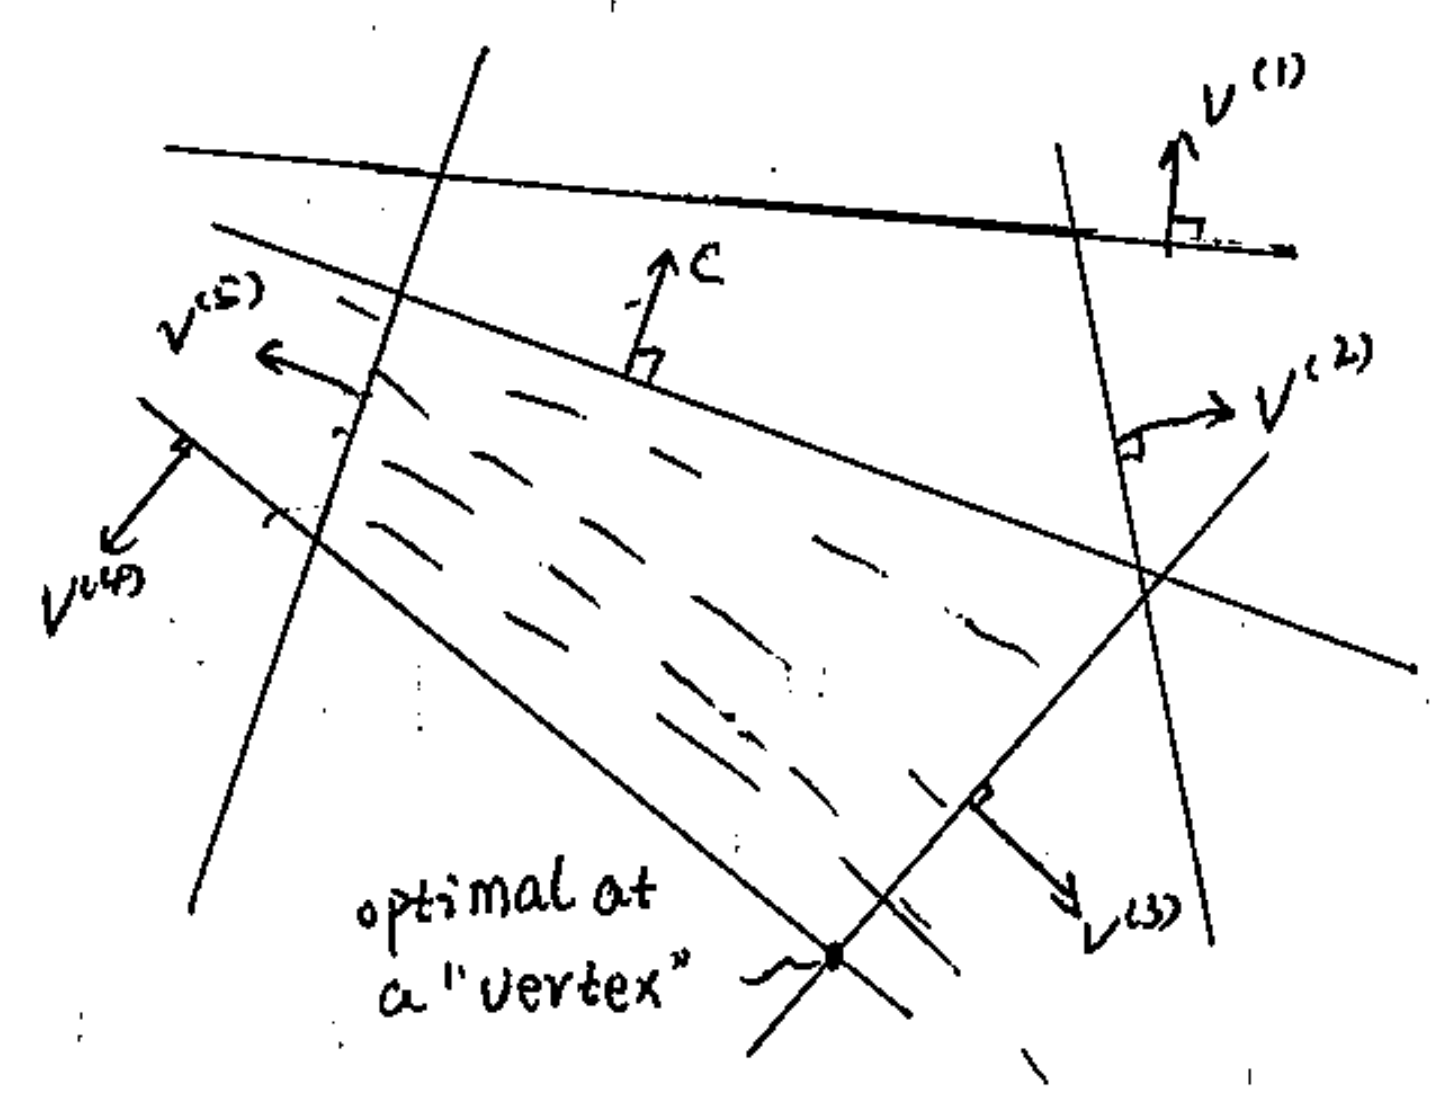
\includegraphics[width=2.1in,height=2.1in]{figures/ch07/figure1012_6.png}
		%\caption{This is an inserted JPG graphic} 
		%\label{fig:graph} 
	\end{figure}
	
	What's optimum? Looks like $x^*=v^{(3)}$.
	
	
	\vspace{0.5cm}
	We may also have a facet with the feasible set 
	$$S = \{x\in \reals^3 | x_1 +x_2+x_3 = 1, x_1 \geq 0, x_2\geq 0,x_3\geq 0\}$$
	
	
	\begin{figure}
		\centering
		\includegraphics[width=2.1in,height=2.1in]{figures/ch07/figure1012_7.png}
		%\caption{This is an inserted JPG graphic} 
		%\label{fig:graph} 
	\end{figure}
	
	So there are various possibilities here for $p^*$ and  $x^* $:
	
	\begin{itemize}
		\item 1) $x^*$ is unique, $p^*$ finite
		
		\item 2) $x^*$ is not unique, $p^*$ finite. 
		
		\item 3) There is no $x^*$:
		
		\quad a) $S = \emptyset$ (Feasible set is empty), constraint $p^* = \infty$. So we say that this LP problem is infeasible.
		
		\quad b) $S$ is unbounded \& no minimum, constraint $p^* = -\infty$
	\end{itemize}
	
	
	\begin{figure}
		\centering
		\includegraphics[width=2.1in,height=2.1in]{figures/ch07/figure1012_8.png}
		%\caption{This is an inserted JPG graphic} 
		%\label{fig:graph} 
	\end{figure}
	
	Active constraints: An optimal solution that lies at the intersection point of two constraints causes both of those constraints to be considered active
	
	Inactive constraints: If any of the constraint lines do not pass through the optimal point, those constraints are called inactive.
	
	In this example(see picture above) constraints g(1) and g(2) are active at optimum.
	
	Note that, we could improve(decrease) the cost if:
	$$c^{\trans}(x^{(0)} + \bigtriangleup) + d < c^{\trans}x^{(0)} + d$$
	That is, $\langle c, \bigtriangleup\rangle < 0$, the angle between displacement vector $\bigtriangleup$ and normal vector $c$ is an obtuse angle(see the picture above).
\end{example}





\vspace{0.5cm}
Some observations:
\begin{itemize}
	\item If you are at a vertex(doesn't have to be optimum). 
	
	\item Any "move" that keeps you feasible must also let you move into the feasible set 
	
	$\rightarrow$ opposite vector that define active constraints.
	
	\begin{equation*}
		v - \alpha g^{(1)} - \beta g^{(2)}, \quad \alpha, \beta \geq 0
	\end{equation*}
	
	\item Are these any choices of $\alpha, \beta$ that decrease the cost?
	\begin{align*}
		c^{\trans}(v - \alpha g^{(1)} - \beta g^{(2)}) + d &\leq c^{\trans}x + d\\
		-\alpha \langle c, g^{(1)}\rangle  - \beta \langle c, g^{(2)}\rangle &\leq 0
	\end{align*}
\end{itemize}

If:

1) $\langle c, g^{(1)}\rangle < 0$

2) $\langle c, g^{(2)}\rangle < 0$

no more into feasible set will decrease the cost.\\ 

\vspace{0.5cm}
Condition for optimality:

A feasible vertex $v$: $v\in\{x|Gx \leq h \}$ is an optimal solution to LP with cost $F_0(x) = c^{\trans}x + d$ if $c^{\trans}g^{(i)} < 0$, $\forall i\in$ active set.\\

\begin{figure}
	\centering
	\includegraphics[width=2.1in,height=2.1in]{figures/ch07/figure1012_9.png}
	%\caption{This is an inserted JPG graphic} 
	%\label{fig:graph} 
\end{figure}


\subsection{Simplex Algorithm}
Simplex algorithm:
\begin{itemize}
	\item 1) Start from a feasible vertex;
	
	\item 2) Identify direction of cost decrease along an edge;
	
	\item 3) Move on that direction until any further more would violate a previously inactive constraints.
	
	\item 4) Stop + add that new constraint(s) to active set.
	
	\item 5) Repeat
\end{itemize}




%\begin{equation*}
%\{x|Gx\leq h \}
%\end{equation*}


%\begin{figure}
%	\centering
%	\includegraphics[width=2.1in,height=2.1in]{figures/ch07/figure1016_1.png}
%\caption{This is an inserted JPG graphic} 
%\label{fig:graph} 
%\end{figure}


%If $x =v^{(a)}$, constraints, constraints 1\&2 active, 3 is inactive.

%\begin{align*}
%<g^{(1)}, v^{(a)}> &= h_1\\
%<g^{(2)}, v^{(a)}> &= h_2\\
%<g^{(3)}, v^{(a)}> &< h_3
%\end{align*}

%At $x = v^{(b)}$, constraints 2\&3 active, 1 is inactive.\\

%1) Define a vertex $v$:

%\begin{itemize}
%	\item a) $v\in S$ is a vertex if cannot express $v = \lambda u +(1-\lambda)w$, $u, w\in S$, $\lambda \in [0,1]$

%	\item b) There exists a cost vector $c\in \reals^n$ s.t. $v$ is unique solution to an LP with cost vector $c$.

%	\item c) Algebraic characterization of vertices in terms of $A, b, G, h$. $S = \{x|Ax \leq b, Gx\leq h \}$
%\end{itemize}



%2) Define / Find directions along edges of polyhedron that keep you in the feasible set.

%3) How far can you go in direction that decrease cost until "leave" feasible set?


\begin{example}
	Consider the problem:
	\begin{align*}
		&min \Vert Ax - b\Vert_{\infty}\\
		&s.t. Gx \leq h
	\end{align*}
	
	Recall that $\Vert u\Vert_{\infty} = max_{i\in [n]}|u_i|$,
	\begin{figure}
		\centering
		\includegraphics[width=2.1in,height=2.1in]{figures/ch07/figure1016_2.png}
		%\caption{This is an inserted JPG graphic} 
		%\label{fig:graph} 
	\end{figure}
	
	Introduce a helper(auxiliary) variable $t\in \reals$ which corresponding to the value of the norm, so the we convert the original problem into following problem:	
	\begin{align*}
		min &\qquad t\\
		s.t. &Ax - b\leq t\textbf{1}\\
		&Ax - b\geq (-t)\textbf{1}\\
		&Gx \leq h
	\end{align*}
\end{example}


\begin{example}
	Consider the problem:
	\begin{align*}
		\min_x &\Vert Ax - b\Vert _1, \qquad A\in \reals^{q\times n}\\
		s.t. &Gx\leq h
	\end{align*}
	\begin{figure}
		\centering
		\includegraphics[width=2.1in,height=2.1in]{figures/ch07/figure1016_3.png}
		%\caption{This is an inserted JPG graphic} 
		%\label{fig:graph} 
	\end{figure}
	
	Recall the definition of $L_1$ norm:
	\begin{equation*}
		\Vert u\Vert_1 = \sum^q_{i=1} |u_i|
	\end{equation*}
	
	%	\begin{figure}
	%		\centering
	%		\includegraphics[width=2.1in,height=2.1in]{figures/ch07/figure1016_4.png}
	%		%\caption{This is an inserted JPG graphic} 
	%		%\label{fig:graph} 
	%	\end{figure}
	
	Let's introduce the helper vector $t\in \reals^q$,
	\begin{align*}
		\min_{x,t} &\sum^q_{i=1}t_i\\
		s.t. \quad&Gx \leq h\\
		&Ax -b \leq t\\
		&Ax -b \geq -t
	\end{align*}
	
\end{example}



\begin{example}
	Consider following problem:
	\begin{align*}
		min \quad max_{i\in [q]} &(c^{(i)^{\trans}}x + d_i)\\
		s.t. &Gx\leq h
	\end{align*}
	This case is similar to the $L_\infty$ norm case due to the inner max function, but it is one-sided(no lower bound). So we could convert the original one to the following:
	\begin{align*}
		min  &\qquad t\\
		s.t. &(c^{(i)^{\trans}}x + d_i)\leq t,\quad \forall i\in [q]\\
		&Gx\leq h
	\end{align*}
	\begin{marginfigure}
		\centering
		\includegraphics[width=2.1in,height=2.1in]{figures/ch07/figure1016_5.png}
		%\caption{This is an inserted JPG graphic} 
		%\label{fig:graph} 
	\end{marginfigure}
\end{example}

Remark:

In above three examples, the decision variables in initial formulation are $x\in \reals^n$, but in reformulation they become:

Example 7.6: $(x, t) \in \reals^n \times \reals$

Example 7.7: $(x, t) \in \reals^n \times \reals^n$

Example 7.8: $(x, t) \in \reals^n \times \reals$



\begin{example}
	Finding the largest $L_2$ ball that fits in a polytope.
	
	Let $p = \{x\in \reals^n| Gx\leq h \}$,
	
	\begin{figure}
		\centering
		\includegraphics[width=2.1in,height=2.1in]{figures/ch07/figure1016_6.png}
		%\caption{This is an inserted JPG graphic} 
		%\label{fig:graph} 
	\end{figure}
\end{example}

It turns out that, this problem can be formulated as an LP problem. \

Note that:
\begin{itemize}
	\item A sphere is fully parameterized by its center $x_c$ and its radius $r$
	
	\item A sphere $(x_c, r)$ fits in $p$ if: $x_c + u \in p$, $\forall u \quad s.t. \Vert u\Vert _2\leq r$
\end{itemize}

\vspace{0.3cm}
Now, let's formulate as an LP. To accomplish this, observe that 

$x_c+u \in p$ means that $g^{(i)^{\trans}}(x_c + u) \leq h_i,\quad \forall i\in [q]$, $\forall u$ s.t. $\Vert u\Vert _2\leq r$.

\vspace{0.2cm}
Examine the constraint $g^{({i})^{\trans}}x_c + g^{({i})^{\trans}}u \leq h_i$ at a time:

As for $g^{({i})^{\trans}}u$, what's the direction of $u$ in order to make this term large as possible? It turns out, $u$ must be aligned with $g^{(i)}$, the same direction with $g^{(i)}$.

Furthermore, what's the value of $u$ that is aligned with $g^{(i)}$ and satisfies  $\vert u\vert_2=r?$ It should be:
$$u^*=\frac{g^{(1)}}{\Vert g^{(1)}\Vert }r$$


So, if the following is satisfied:
$$g^{(i)^{\trans}}[x_c + u^*] \leq h_i$$\
Then constraint $i$ will be satisfied for all $u$ such that $\vert u\vert \leq r$.

Substituting in $u^*$, the constraints become:
$$g^{(i)^{\trans}} x_c + \Vert g^{(i)}\Vert_2 r\leq h_i$$
Note that the constraint is linear in $x_c$ and $r$.

The problem of finding the largest sphere becomes the following:
\begin{align*}
	\max \quad & r\\
	s.t.\quad &g^{(i)^{\trans}}x_c + r \Vert g^{(i)}\Vert _2\leq h_i \qquad \forall i\in [q]
\end{align*}


Remarks:

(1) Optimal value $(x_c, r)\in \reals^{n+1}$.

(2) $x_c$ is a variable that does not enter the objective.

(3) Possibly no solution if $p$ is an empty set.

(4) Constraints and objective are linear in optimal variable so it is an LP problem.

(5)Transformed some quadratic-like problem (quadratic as a sphere is involved) into an LP, because we were able to identify which direction of $u$ the worst case for each constraint.






\newpage

\section{Quadratic program(QP)}

A quadratic programming problem is formulated in a general way as follows
\begin{align*}
p^* = \min_{x\in \reals^n}\quad &\frac{1}{2}x^{\trans}Hx + c^{\trans}x + d\\
 s.t.\quad &Ax = b\\
 &Gx\leq h
\end{align*}

The feasible set(feasible region) is illustrated as follows
\begin{figure}
	\centering
	\includegraphics[width=2.1in,height=2.1in]{figures/ch07/figure1016_a.png}
	%\caption{This is an inserted JPG graphic} 
	%\label{fig:graph} 
\end{figure}

\subsection{Connection between LS problem and QP problem}
Recall the lest square problem we have studied, it turns out that we can convert the least square problem into a QP problem.
\begin{align*}
\Vert Ax - y\Vert _2^2 &= (Ax - y)^{\trans}(Ax - y)\\
&= x^{\trans}A^{\trans}Ax - 2y^{\trans}Ax + y^{\trans}y\\
&= \frac{1}{2}x^{\trans}(2A^{\trans}A)x - 2y^{\trans}Ax + \Vert y\Vert _2^2
\end{align*}

However, for the converse case, we can not always manipulate the objective of a QP into a  LS problem.


\subsection{Equality constrained QPs: Substitute back to the objective}
A basic idea of solving such kind of problem is to substitute the equality constraints back to the objective function so that hopefully we can eliminate some variables(dimensions), and obtain an unconstrained QP problem.

Consider a formulation of such kind of problem,
\begin{align*}
p^* = min_{x\in \reals^n}\quad &\frac{1}{2}x^{\trans}Hx + c^{\trans}x + d\\
s.t.\quad &Ax = b
\end{align*}


\begin{figure}
	\centering
	\includegraphics[width=2.1in,height=2.1in]{figures/ch07/figure1016_b.png}
	%\caption{This is an inserted JPG graphic} 
	%\label{fig:graph} 
\end{figure}

The feasible set could be expressed as follows
$$\mathcal{A} =\{x | x = \bar{x} + \xi,\quad \text{where } \xi \in N(A) \}$$
where $\bar{x}$ is a particular solution to the equation $Ax=b$.

Let $N$ be a basis for $N(A)$, so that we can express $\xi \in N(A)$ as $\xi = Nz$, where $z\in \reals^k$, $k =\text{dim}(N(A)) \leq n$.

Substitute this expression for any feasible $x$ into the objective $F_0(\cdot)$
\begin{align*}
F_0(x) 
&= F_0(\bar{x} + \xi)\\
&= F(\bar{x} + Nz)\\
&= \frac{1}{2}(\bar{x} + Nz)^{\trans}H(\bar{x}+Nz) + c^{\trans}(\bar{x} + Nz) + d\\
&= \frac{1}{2}z^{\trans}[N^{\trans}HN]z + [c^{\trans}N + \bar{x}^{\trans}HN]z + [\frac{1}{2}\bar{x}^{\trans}H\bar{x} + c^{\trans}x + d] \\
&= \frac{1}{2}z^{\trans}\tilde{H}z + \tilde{c^{\trans}}z + \tilde{d}\\
\end{align*}
where we newly define $\tilde{H}$, $\tilde{c^{\trans}}$, and $\tilde{d}$ in the last equality. So now we have obtain an unconstrained QP problem which is formulated as
\begin{equation*}
p^* = min_{z\in \reals^k}\quad \frac{1}{2}z^{\trans}\tilde{H}z + \tilde{c^{\trans}}z + \tilde{d}
\end{equation*}

Hence, to summarize,

(1)We have got a newly lower-dimensional optimization problem since $k =\text{dim}(N(A)) \leq n $.

(2)The new problem is still a QP, but is an unconstrained QP.



\begin{example}{Markowitz Portfolio optimization/Mean/variance" analysis}  Harry Markowitz(1990 Nobel Prize)
	
	
	\textbf{Problem formulation}: 
	\begin{itemize}
		\item Objective: For a fixed level of (expected) returns, we want to minimize the variance of returns.
		
		\item There are $n$ stocks, and we only consider a single investment period\\
		
		\item Design an optimal investment strategy $p\in \reals^n$, where the component $p_i = $ is the weight of your total wealth invested in the stock $i$.
		
		\item We require $\sum^n_{i=1}p_i = 1$, that is, you must invest all your money.
		
		\item We also require $p_i \geq 0$, that is, you are only allowed to take long positions, and short selling is not allowed.
		
		\item Your total wealth is normalized to $1$. So $p_i$ is not only weight but also the amount of money you invest on stock $i$ now.
	\end{itemize} 
	
	\textbf{Return and Variance}:
	
	\begin{itemize}
		\item Let $x\in \reals^n$ be a random vector denotes the return of $n$ stocks, so component $x_i$ is the return on the $i$-th stock in one period. That is, if we invest 1 RMB in a stock at the beginning, we will get $x_i$ RMB back at the end of this period.

		\item Expected returns: $\bar{x_i} = \mathbb{E}[x_i]$. In general, it is a known estimator based on historical data.
		
		\item Your return (random) is $\sum^n_{i=1}p_ix_i = p^{\trans}x$
		
		\item Your expected return $\mathbb{E}[\sum^n_{i=1}p_ix_i] = \sum^n_{i=1}p_i\mathbb{E}[x_i] = \sum^n_{i=1}p_i\bar{x_i} = p^{\trans}\bar{x}$
		
		\item variance in your return:
		\begin{align*}
		var(p^{\trans}x) &=\mathbb{E}[(p^{\trans}x - p^{\trans}\bar{x})^2]\\
		&= \mathbb{E}[(p^{\trans}(x - x^{\trans}))^2]\\
		&= \mathbb{E}[p^{\trans}(x - \bar{x})(x - \bar{x})^{\trans}p]\\
		&= p^{\trans}\mathbb{E}[(x - \bar{x})(x - \bar{x})^{\trans}]p\\
		&= p^{\trans}\Sigma p
		\end{align*}
	\end{itemize}
	
	
	With above terminology and model formulation, given a mean return $\bar{x}$ and the covariance matrix of returns $\Sigma \in \reals^{n\times n}$, we want to find an optimal strategy/policy $p$ to minimize the risk(represent by variance) subject to same minimal returns.: 
	
	The problem is formulated as:
	\begin{align*}
	min_{p\in \reals^n}\quad &p^{\trans}\Sigma p\\
	s.t. \quad&p^{\trans}\bar{x}\geq r_{min}\\
	&\textbf{1}^{\trans}p = 1\\
	&p\geq 0
	\end{align*}
\end{example}



\subsection{Geometry of QP}
Consider the general form of QP
\begin{align*}
p^* = min_{x\in \reals^n}\quad &\frac{1}{2}x^{\trans}Hx + x^{\trans}x + d\\
s.t.\quad &Ax = b\\
&Gx\leq h
\end{align*}
Follow the same as LP, we would like to discuss the geometry of QP.

\begin{marginfigure}
	\centering
	\includegraphics[width=2.5in,height=3in]{figures/ch07/figure1112_01.png}
	\caption{Plot 1} 
	%\label{fig:graph} 
\end{marginfigure}


\begin{marginfigure}
	\centering
	\includegraphics[width=2.5in,height=3in]{figures/ch07/figure1112_02.png}
	\caption{Plot 2} 
	%\label{fig:graph} 
\end{marginfigure}


\begin{marginfigure}
	\centering
	\includegraphics[width=2.5in,height=3in]{figures/ch07/figure1112_03.png}
	\caption{Plot 3} 
	%\label{fig:graph} 
\end{marginfigure}

(1) Geometry of feasible set: The same as LP.

(2) Geometry of objective: Without loss of generality(w.l.o.g), we can assume that $H\in S^n$, i.e., $H$ is symmetric, since
\begin{align*}
x^{\trans}Hx 
&=\frac{1}{2}[x^{\trans}Hx + x^{\trans}H^{\trans}x]\\
&= \frac{1}{2}x^{\trans}(H+H^{\trans})x
\end{align*}
clearly $H$ is symmetric.\\

Recal that for symmetric matrices, we have

a) Eigenvalues: purely real eigenvalues (so we can arrange them in an order).

b) Eigenvectors: can be chosen to be $\perp$ and can always diagonalize $H$, i.e., we can write
$$H = \mathcal{U}\Lambda \mathbb{U}^{\trans}  = \sum^n_{i=1}\lambda_iu^{(i)}u^{(i)^{\trans}}$$

Consider following 3 different cases for the matrix $H$:
\begin{itemize}
	\item A) $H\in S^n$ but not PSD
	
	\begin{equation*}
	H = 
	\begin{bmatrix}
	1&0\\
	0&-2
	\end{bmatrix}
	\end{equation*}
	
	\item B) $H\in S^n_+$ but not PD
	\begin{equation*}
	H = 
	\begin{bmatrix}
	1&0\\
	0&0
	\end{bmatrix}
	\end{equation*}
	
	\item C) $H\in S^n_{++}$
	\begin{equation*}
	H = \begin{bmatrix}
	1&0\\
	0&2
	\end{bmatrix}
	\end{equation*}
\end{itemize}

%Now, let's look at visualization for cases A to C.

%If we only consider the quadratic term,
%$$F_0(x) =\frac{1}{2}x^{\trans}Hx$$
%Clearly, we have following results

Consider the 3 cases for $H$ given above and the following different objective functions, we plot these figures on r.h.s. for illustration.

Plot 1: $F_0(x) =\frac{1}{2}x^{\trans}Hx$

Plot 2: $F_0(x) =\frac{1}{2}x^{\trans}Hx + [0.5\quad 0.5]x$

Plot 3: $F_0(x) =\frac{1}{2}x^{\trans}Hx + [0.5\quad 0]x$


\vspace{0.5cm}
\textbf{Let's consider 3 different cases for a general QP problem.}

\textbf{Case A: } $H\in S^n$ but $H\notin S^n_+$ (Symmetric not PSD).

For such $H$, there must be an eigenvalue/vector pair $(\lambda, u)$ s.t. $\lambda < 0$.

Set $x_{\alpha} = \alpha u$ for some $\alpha \in \reals$, we have

\begin{align*}
F_0(\alpha u) &= \frac{1}{2}(\alpha u)^{\trans}H(\alpha u) + c^{\trans}(\alpha u) + d\\
&= \frac{{\alpha}^2}{2} u^{\trans}[\sum^n_{i=1}\lambda_i u^{(i)} u^{(i)^{\trans}}]u + \alpha c^{\trans}u + d\\
&= \frac{{\alpha}^2}{2}\lambda + \alpha <c,u> + d
\end{align*}

Since $\lambda<0$, let $\alpha \to \infty$ leads to an unbounded objective function, i.e., $p^* = -\infty$.



\vspace{0.3cm}
\textbf{Case B: } $H\in S_+^n$ but $H\notin S^n_{++}$ ($H$ is PSD but not PD)

$\rightarrow$ $H$ has at least 1 zero eigenvalue.\\

\vspace{0.3cm}
\textbf{Case B (i)} $H\in S_+^n$ but $H\notin S^n_{++}$ and $c \notin R(H)$.

There is a complement of $c$ in $R(H)^{\perp} = N(H^{\trans}) = N(H)$, and thus we can move in that direction without affecting $2^{nd}$ order term while driving $1^{st} $ order term to $-\infty$.

Let $c_{\Vert} = \prod_{R(H)}(c)$,  and $c_{\perp} = \prod_{N(H)}(c)$, where the first one is the component in $R(A)$ and second one is the component in $N(H)$.

Notice that $R(H)^{\perp}= N(H^{\trans}) = N(H)$, since $H$ is symmetric. By orthogonal decomposition lemma, there is an unique decomposition
$$c = c_{\Vert} + c_{\perp}$$

Now, let $x_{\alpha} =-\alpha c_{\perp}$, where $\alpha \in \reals_+$.
\begin{align*}
F_0(x_{\alpha}) 
&=\frac{{\alpha}^2}{2}c_{\perp}^{\trans}Hc_{\perp} + c^{\trans}(-\alpha c_{\perp}) + d\\
&= 0 - \alpha(c_{\Vert} + c_{\perp})^{\trans}c_{\perp} + d\\
&= -\alpha(c_{\Vert}^{\trans}c_{\perp} + c_{\perp}^{\trans}c_{\perp}) + d\\
&= -\alpha \Vert c_{\perp}\Vert^2_2 + d
\end{align*}

Hence the function is unbounded below since we could take $\alpha \to\infty$. Therefore,
$$p^*=-\infty$$



\vspace{0.3cm}
\textbf{Case B (ii)}  $H\in S_+^n$ but $H\notin S^n_{++}$ and $c \in R(H)$.

First, remind us of some results from previous chapter,
\begin{align*}
H 
&= \sum^n_{i=1}\lambda_i U^{(i)}U^{(i)^{\trans}} \\
&= \sum^r_{i=1}\lambda_i U^{(i)}U^{(i)^{\trans}}\\
&= U_r\Sigma Y_r^{\trans}
\end{align*}
and,
\begin{align*}
H^{\frac{1}{2}} &= U_r\Sigma^{\frac{1}{2}}U_r^{\trans}\\
H^{+} &= U_r\Sigma^{-1}U_r^{\trans}\\
(H^{\frac{1}{2}})^+ &= U_r\Sigma^{-\frac{1}{2}}U_r^{\trans}
\end{align*}

where 
$$\Sigma = 
\begin{bmatrix}
\sqrt{\lambda_1} &  & 0 \\
&\ddots&\\
0&&\sqrt{\lambda_r}
\end{bmatrix}
,\
\Sigma^{-\frac{1}{2}} =
\begin{bmatrix}
\frac{1}{\sqrt{\lambda_1}} &  & 0 \\
&\ddots&\\
0&&\frac{1}{\sqrt{\lambda_r}}
\end{bmatrix}
$$

Observe that
$$C\in R(H) = R(H^{\frac{1}{2}}) = R(H^+) = R\left((H^{\frac{1}{2}})^+\right)$$

Since $C\in R(H)$ and $R(H) = R(H^{\frac{1}{2}})$, there exists $y \in \reals^n$ such that
$$C = H^{\frac{1}{2}}y = H^{\frac{1}{2}}(y+\xi)$$

where $\xi \in N(H^{\frac{1}{2}})$. Note that choice of $y$ is not unique and the second equality due to $\rank(H)= r<n$. 

Explicitly, we have 
\begin{equation*}
C = (U_r\Sigma^{\frac{1}{2}}U_r^{\trans})y = \sum^r_{i=1}U^{(i)}\sqrt{\lambda_i}(U^{(i)^{\trans}}y)
\end{equation*}

Now, the question is, which $y$ we should pick? Let's pick the $y$ with min-norm, that is, 
\begin{align*}
y &=\arg\min_{\bar{y}\in\reals^n}\Vert \bar{y}\Vert_2\\
s.t\  C &= H^{\frac{1}{2}}\bar{y}
\end{align*}

It turns out that, this is an under determined and rank-deficient LS problem. So the solution to this question is given by
$$y = (H^{\frac{1}{2}})^+C = U_r \Sigma^{-\frac{1}{2}} U_r^{\trans} C$$


So, when $C = H^{\frac{1}{2}}y$, we can pick $y = (H^{\frac{1}{2}})^+C$. Let's look back at the objective to understanding such choice.
\begin{align*}
\frac{1}{2}x^{\trans}Hx + c^{\trans}x + d &= \frac{1}{2}x^{\trans}H^{\frac{1}{2}}H^{\frac{1}{2}}x+y^{\trans}H^{\frac{1}{2}}x + d\\
&= \frac{1}{2}\tilde{x}^{\trans}\tilde{x} + y^{\trans}\tilde{x} + d\\
&= \frac{1}{2}(\tilde{x}^{\trans}x+2y^{\trans}\tilde{x}+y^{\trans}y) - \frac{1}{2}y^{\trans}y + d \\
&= \frac{1}{2}\Vert\tilde{x}+y\Vert^2_2 - \frac{1}{2}\Vert y \Vert^2_2 + d &(*)
\end{align*}
In the second equality we let $\tilde{x} = H^{\frac{1}{2}} x$.

Apparently, we would like to set $\tilde{x} = -y$ to minimize $(*)$, and the question is, is this always possible? The answer is yes.

Since $y = (H^{\frac{1}{2}})^+C\in R((H^{\frac{1}{2}})^+) = R(H) = R(H^{\frac{1}{2}})$, and $\tilde{x}=H^{\frac{1}{}} x$ so $\tilde{x} \in R\left(H^{\frac{1}{2}}\right) = R(H)$. Since $x\in \reals^n$ is unconstrained, so we can choose $x$ to make $\tilde{x}$ equal to any element of $R(H)$, namely $y$. 

Thus, to minimize $(*)$ we set $\tilde{x} = -y$ where $\tilde{x} = H^{\frac{1}{2}}x$, and yields
\begin{align*}
F_0(x) \geq p^* &= d - \frac{1}{2}\Vert y \Vert_2^2\\
&= d - \frac{1}{2}y^{\trans}y\\
&= d - \frac{1}{2}C^{\trans}(H^{\frac{1}{2}})^+(H^{\frac{1}{2}})^+C\\
&= d - \frac{1}{2}C^{\trans}
\begin{bmatrix}
U_r
\end{bmatrix}
\begin{bmatrix}
\Sigma^{-\frac{1}{2}}]
\end{bmatrix}
\begin{bmatrix}
U_r^{\trans}
\end{bmatrix}
\begin{bmatrix}
U_r
\end{bmatrix}
\begin{bmatrix}
\Sigma^{-\frac{1}{2}}]
\end{bmatrix}
\begin{bmatrix}
U_r^{\trans}
\end{bmatrix}
\begin{bmatrix}
C
\end{bmatrix}\\
&= d - \frac{1}{2}C^{\trans}(U_r\Sigma^{-1}U^{\trans}_r)C\\
&= d - \frac{1}{2}C^{\trans}H^+C
\end{align*}

What is the minimizing choice of $x\in \reals^n$?

Since $y\in R(H) = R(H^{\frac{1}{2}})$ and $x\in \reals^n$ is free, we can satisfy equality and thus there are many solutions. 

We would like to pick min-norm solution for $x$, which is given by
\begin{align*}
x^* 
&= (H^{\frac{1}{2}})^+\tilde{x}\\
&= -(H^{\frac{1}{2}})^+y\\
&= -(H^{\frac{1}{2}})^+(H^{\frac{1}{2}})^+C\\
&= -H^+C
\end{align*}\\

\vspace{0.3cm}
\textbf{Case C}: $H\in S^n_{++}$ ($H$ is PD)

This is indeed a special case of case B(ii), and that's because

(1)$H\in S^n_{++}$, then it is also in $S^n_{+}$, and so all eigenvalues are non negative.

(2)$H\in S^n_{++}$, then $\rank(H) = n$ and thus $R(H)=\reals^n$, and certainly $C \in R(H)$.

From previous solution, we have
\begin{align*}
x 
&= -H^{+}C\\
&= -U_r \Sigma^{-1} U_r^{\trans} C\\
&= -U_r \Sigma^{-1} U_n^{\trans} C\\
&= - H^{-1} C
\end{align*}
So in this case $H^+ = H^{-1}$. The optimal value is given by
$$p^* = d - \frac{1}{2}C^{\trans}H^{-1}C$$


\textbf{Summary }

Consider the QP problem $p^* = min_{x\in \reals^n}\frac{1}{2}x^{\trans}Hx + c^{\trans}x + d$,
\begin{equation}
p^* = \left\{
\begin{array}{lr}
d - \frac{1}{2}c^{\trans}H^+c &\text{$H$ is PD, or, $H$ is PSD but not PD and $c \in R(H)$}\\
-\infty &\text{$H$ is not PSD, or, $H$ is PSD but not PD and $c\notin R(H)$}
\end{array}
\right.\nonumber
\end{equation}

\begin{equation}
x^* = \left\{
\begin{array}{lr}
-H^+c &\text{$H$ is PD, or, $H$ is PSD but not PD and $c \in R(H)$}\\
\text{not exist} &\text{$H$ is not PSD, or, $H$ is PSD but not PD and $c\notin R(H)$}
\end{array}
\right.\nonumber
\end{equation}

\vspace{0.5cm}
\subsection{Solving QPs via "active set" methods}

\begin{align*}
\min_{x\in \reals^2} \quad & (x_1 - 1)^2 + (x_2 - 2.5)^2 \\
s.t. \quad&
\begin{bmatrix}
-1&2\\
1&2\\
1&-2\\
-1&0\\
0&-1
\end{bmatrix}
\begin{bmatrix}
x_1\\
x_2
\end{bmatrix}
\leq
\begin{bmatrix}
2\\
6\\
2\\
0\\
0
\end{bmatrix}
\end{align*}

\begin{marginfigure}
	\centering
	\includegraphics[width=1.8in,height=1.8in]{figures/ch07/figure1021_1.png}
	%\caption{This is an inserted JPG graphic} 
	%\label{fig:graph} 
\end{marginfigure}

\begin{itemize}
	\item at optimum some subset of inequality constraints satisfied with equality "active" set
	
	\item Best "loose"
	
	\item If you know the active set or optimum, just solve an "equality"-constrained QP"
\end{itemize}
By illustrative example:

Step 1

Initialize at point $x^{(0)} = \begin{bmatrix}
2\\
0
\end{bmatrix}$, starting with initial "working set" of equality constraint(the fifth equality constraint):
$$w_0 = \{x|x_2 = 0 \}$$


Step 2
 \begin{align*}
\min_{x\in \reals^2} \quad
&
\frac{1}{2}x^{\trans}
\begin{bmatrix}
2&0\\
0&2
\end{bmatrix}
x + 
\begin{bmatrix}
-2 & -5
\end{bmatrix} 
+ (1 + 2.5^2)\\
s.t.\quad &
\begin{bmatrix}
0 & 1
\end{bmatrix}
x = 0
\end{align*}


Recall the linearly constrained QP problem, we need a basis for 
$N(\begin{bmatrix} 
0\\
1
\end{bmatrix}) 
= \{x|x = \alpha
\begin{bmatrix}
1\\
0
\end{bmatrix} \}$
in this case. Let
$N=
\begin{bmatrix}
1\\
0
\end{bmatrix}$,

$$\tilde{H} = N^{\trans}HN = 2$$
$$\tilde{C}^{\trans} = (c^{\trans}N + \bar{x}^{\trans} HN)= -2$$
$$\tilde{d}= (d+c^{\trans}x + \frac{1}{2}\bar{x}^{\trans}H\bar{x})=0$$


So we have converted the problem to :
\begin{align*}
z^* 
&= \arg\min_{z\in\reals} \frac{1}{2} z^{\trans}\tilde{H}z + \tilde{c}^{\trans}z + \tilde{d}\\
&= \arg\min_{z\in\reals} \frac{1}{2}2z^2 + (-2z)+ 0\\
&= \arg\min_{z\in\reals} z^2 - 2z
\end{align*}
Take the first derivative and set it to zero, we get $z^* = 1$.

So the optimum is:
\begin{equation*}
x^{(1)}= \bar{x}+ z^*N = 
\begin{bmatrix}
0\\
0
\end{bmatrix}
 + 1
\begin{bmatrix}
1\\
0
\end{bmatrix} = 
\begin{bmatrix}
1\\
0
\end{bmatrix}
\end{equation*}


Step 3

Note:

(1) At this point we recognize that the equality constraint $\{x|x_2=0\}$ is no longer "binding" because we just optimized along that set.

(2) We could drop the fifth constraint from "working set" left with $w_2 =\emptyset$

(3) We are facing with an unconstrained optimization problem. Clearly we would like to move to $x^{(1)} +\Delta = 
\begin{bmatrix}
1\\
0
\end{bmatrix}
+
\begin{bmatrix}
0\\
2.5
\end{bmatrix}
$.

(4) But there may be a "blocking" constraint in way. In this example, this is the first constraint $\{x|-x_1 +2x_2\leq 2 \}$

(5) Instead, we solve for the a step size $\gamma$ to make the constraint light, i.e., $g^{(i)T}(x^{(1)}+\gamma \Delta) = h_1$. 

So we have,
$$[-1\ 2] 
\begin{bmatrix}
1\\
0
\end{bmatrix}
+
\gamma
\begin{bmatrix}
0\\
2.5
\end{bmatrix}
=
2
\Leftrightarrow
\gamma= \frac{3}{5}
$$

$$
x^{(2)} = x^{(1)} +\frac{3}{5} \Delta =
\begin{bmatrix}
1\\
1.5
\end{bmatrix}
$$


Step 4

This time, $w_3 = \{x|
\begin{bmatrix}
-1& 2
\end{bmatrix}
\begin{bmatrix}
x_1\\
x_2
\end{bmatrix}
=2
\}$.

$$N(
\begin{bmatrix}
-1& 2
\end{bmatrix})
=
\{x|x=\alpha
\begin{bmatrix}
2\\
1
\end{bmatrix}\},
\quad
\bar{x}\in 
\{x|
\begin{bmatrix}
-1& 2
\end{bmatrix}
\begin{bmatrix}
x_1\\
x_2
\end{bmatrix}
=2
\}
$$

We pick $N=
\begin{bmatrix}
2\\
1
\end{bmatrix}
,\quad
\bar{x}=
\begin{bmatrix}
0\\
1
\end{bmatrix}
$.

$$\tilde{H} = N^{\trans}HN = 10$$
$$\tilde{C}^{\trans} = (c^{\trans}N + \bar{x}^{\trans} HN)= -7$$
$$\tilde{d}= (d+c^{\trans}x + \frac{1}{2}\bar{x}^{\trans}H\bar{x})=-4$$

\begin{align*}
z^* 
&= \arg\min_{z\in\reals} \frac{1}{2} z^{\trans}\tilde{H}z + \tilde{c}^{\trans}z + \tilde{d}\\
&= \arg\min_{z\in\reals} \frac{1}{2}10 z^2 + (-7z) - 4\\
&= \arg\min_{z\in\reals} 5z^2 - 7z -4
\end{align*}
Take the first derivative and set it to zero, we get $z^* = \frac{7}{10}$.

\begin{equation*}
x^{(3)}= \bar{x}+ z^*N = 
\begin{bmatrix}
0\\
1
\end{bmatrix}
+ 
\frac{7}{10}
\begin{bmatrix}
2\\
1
\end{bmatrix} = 
\begin{bmatrix}
1.4\\
1.7
\end{bmatrix}
\end{equation*}

Note $x^{(3)}$ is the global optimum so we end this algorithm here.



\vspace{0.5cm}
\subsection{Quadratically Constrained Quadratic Program (QCQP)}
Let's formulate such kind of problem first
\begin{align*}
\min_{x\in \reals^n} \quad &\frac{1}{2}x^{\trans}H_0 x + c_0^{\trans} x + d_0\\
s.t.\quad &\frac{1}{2}x^{\trans}H_ix + c^{\trans}_i x + d_i \leq 0  & i\in [m]\\
&\frac{1}{2} x^{\trans} \tilde{H}_ix + \tilde{c}_i^{\trans}x + \tilde{d}_i = 0 & i\in [q]
\end{align*}

\textbf{Note:}

\begin{itemize}
	\item If $H_i = 0, \forall i\in [n]$, $\tilde{H}_i = 0, \forall i\in [q]$, then we have a $QP$.
	
	\item Typically $H_0\geq 0$, $H_i\geq 0$, $i\in [m]$, and $\tilde{H}_i = 0$, $\forall i\in [q]$, in which case the problem is a convex optimization problem, and thus it is easy to solve as we will discuss in next chapter.
	
\end{itemize}

To see that why $\tilde{H}_i \neq 0$ makes things difficult, let's consider a single  equality constraint $q = 1$, and a scalar problem $x\in \reals$:
$$\tilde{H}_1 = 1 \quad \tilde{c}_i = 0 \quad \tilde{d}_i = -\frac{1}{2}$$
So the equality constraint becomes:
$$\frac{1}{2}x_1^2 + 0 - \frac{1}{2} = 0 \Leftrightarrow x_1^2 = 1 \Leftrightarrow x_1\in\{-1, 1\} $$
Notice that the feasible set is not a continuum of possibilities, i.e., it is a distinct set so the problem is "Combinatorial".





\begin{example}
Let's consider the QCQP with only three inequality constraints ($m=3$).
\begin{marginfigure}
	\centering
	\includegraphics[width=1.8in,height=1.8in]{figures/ch07/figure1021_2.png}
	\caption{Feasible set of constraint 1} 
	%\label{fig:graph} 
\end{marginfigure}

Constraint 1:

\begin{equation*}
H_1=\begin{bmatrix}
2 & 0 \\
0 &\frac{1}{2}
\end{bmatrix}
\qquad 
c_1^{\trans} = \begin{bmatrix}
0 & 0
\end{bmatrix}
\qquad 
d_1 = -1
\end{equation*}

So this constraint can be written as
\begin{align*}
\frac{1}{2}x^{\trans}H_1x + c_1^{\trans}x + d_1 \leq 0 &\Leftrightarrow 2x_1^2 + \frac{1}{2}x_2^2 \leq 2\\
&\Leftrightarrow\frac{x_1^2}{1} + \frac{x_2^2}{4}\leq 1
\end{align*}

It is obviously the feasible set of this constraint corresponds to an ellipse, and by computing the eigenvalues(lengths of major and minor axis) and eigenvectors(directions of major and minor axis) of $H_1$, we are able to draw such feasible set as on the r.h.s.

\begin{marginfigure}
	\centering
	\includegraphics[width=1.8in,height=1.8in]{figures/ch07/figure1021_3.png}
	\caption{Feasible set of constraint 2} 
	%\label{fig:graph} 
\end{marginfigure}

Constraint 2:
\begin{equation*}
H_2=
\begin{bmatrix}
0 & 0\\
0 & 0
\end{bmatrix}
\qquad
c_2^{\trans} = 
\begin{bmatrix}
-1 & 1
\end{bmatrix}
\qquad
d_2 = -1
\end{equation*}

So this constraint can be written as
\begin{equation*}
\begin{bmatrix}
-1 & 1
\end{bmatrix}x\leq 1\Leftrightarrow
\begin{bmatrix}
-1 & 1
\end{bmatrix}
\begin{bmatrix}
x_1\\
x_2
\end{bmatrix}\leq 1\Leftrightarrow x_2\leq 1 + x_1
\end{equation*}

The corresponding feasible set of this constraint is illustrated on r.h.s.

\begin{marginfigure}
	\centering
	\includegraphics[width=1.8in,height=1.8in]{figures/ch07/figure1021_4.png}
	\caption{Feasible set of constraint 3} 
	%\label{fig:graph} 
\end{marginfigure}

Constraint 3:
\begin{equation*}
H_3=
\begin{bmatrix}
0 & 0\\
0 & 2
\end{bmatrix}
\qquad
c_3^{\trans} = 
\begin{bmatrix}
-1 & 0
\end{bmatrix}
\qquad
d_3 = -1 
\end{equation*}

So this constraint can be written as
$$x^2_2 - x_1 - 1\leq 0$$
The corresponding feasible set of this constraint is illustrated on r.h.s.


Put all these 3 constraints together(i.e., find the intersection of above 3 feasible sets), so we can obtain the desired feasible set for this QCQP problem
\begin{marginfigure}
	\centering
	\includegraphics[width=1.8in,height=1.8in]{figures/ch07/figure1021_5.png}
	\caption{Feasible set for this QCQP} 
	%\label{fig:graph} 
\end{marginfigure}
\end{example}



%\chapter{Convexity}
%\label{ch.convex}
%%% Placeholder for chapter on convexity

%Below are notes for Oct23
\section{Linear/affine/convex/conic hulls \& sets}
Given a set of points $x^{(i)} \in \reals^n$, $i\in [m]$

\begin{equation*}
P = \{x^{(1)}, x^{(2)},..., x^{(m)} \}
\end{equation*}

Consider combinations of form $\sum^m_{i=1} \lambda_i x^{(i)}$

1) The "linear" hull: 

\begin{equation*}
\{x|x = \sum^m_{i=1} \lambda_i x^{(i)}, \lambda_i\in \reals, \forall i\in [m] \}
\end{equation*}

2) The "affine" hull: 

\begin{equation*}
\{x|x = \sum^m_{i=1} \lambda_i x^{(i)}, \lambda_i\in \reals, \sum^n_{i=1}\lambda_i = 1 \}
\end{equation*}


3) The "convex" hull: 

\begin{equation*}
\{x|x = \sum^m_{i=1} \lambda_i x^{(i)}, \lambda_i\in \reals, \lambda_i \geq 0, \sum^m_{i=1}\lambda_i = 1 \}
\end{equation*}


4) The "conic" hull: 

\begin{equation*}
\{x|x = \sum^m_{i=1} \lambda_i x^{(i)}, \lambda_i\in \reals, \lambda_i \geq 0 \}
\end{equation*}


\begin{center}
	\begin{tabular}{|c|c|c|}
	\hline  
   & $\lambda_i \geq 0$   & $\sum^m_{i=1}\lambda_i = 1$ \\
	\hline  
Linear&  no  & no \\
	\hline  
Affine&  no  &yes  \\
	\hline 
Covex&  yes  & yes \\
	\hline  
Conic&  yes  &  no\\
	\hline 
\end{tabular}
\end{center}



1) Linear Hull

Linear hull of $P = \text{span}\{x^{(1)},...,x^{(m)} \} =\text{span}(P)$

$\rightarrow$ smallest subspace that contains $P$.

2) Affine hull

Let $P = \{x^{(1)}, x^{(2)} \}$, 
\begin{align*}
x &= \lambda_1x^{(1)} + \lambda_2x^{(2)}\\
&= \lambda_1x^{(1)} + (1-\lambda)_1x^{(1)}\\
&= x^{(2)} + \lambda(x^{(1)} - x^{(2)})
\end{align*}
Hence, $aff(P) = x^{(2)} + \text{span}(x^{(1)} - x^{(2)})$.

\vspace{0.3cm}
Let $P = \{x^{(1)}, x^{(2)}, x^{(3)} \}$,
\begin{align*}
x &= \lambda_1x^{(1)} + \lambda_2x^{(2)} + \lambda_3x^{(3)}\\
&= (1 - \lambda_2 - \lambda_3)x^{(1)} + \lambda_2x^{(2)} + \lambda_3x^{(3)}\\
&= x^{(1)} + \lambda_2(x^{(2)} - x^{(1)}) + \lambda_3(x^{(3)} - x^{(1)})
\end{align*}
Hence,  $aff(P) = x^{(1)} + \text{span}(x^{(2)} - x^{(1)}) + \text{span}(x^{(3)} - x^{(1)})$.


\begin{marginfigure}
	\centering
	\includegraphics[width=1.8in,height=1.8in]{figures/ch08/figure1023_1.png}
	%\caption{This is an inserted JPG graphic} 
	%\label{fig:graph} 
\end{marginfigure}

3) Convex hulls

Let $P = \{x^{(1)},  x^{(2)}\}$,
\begin{align*}
x 
&= \lambda_1x^{(1)} + \lambda_2x^{(2)}\\
&= (1-\lambda)x^{(1)} + \lambda x^{(2)}\\
&= x^{(1)} + \lambda(x^{(2)} - x^{(1)})
\end{align*}


Let $P = \{x^{(1)},  x^{(2)}, x^{(3)} \}$,
\begin{align*}
x 
&= \lambda_1x^{(1)} + \lambda_2x^{(2)} + \lambda_3x^{(3)}\\
&= x^{(1)} + \lambda_2(x^{(2)} - x^{(1)}) + \lambda_3(x^{(3)} - x^{(1)})\\
&= x^{(1)} + \lambda \gamma(x^{(2)} - x^{(1)}) + (1 - \lambda)\gamma(x^{(3)} - x^{(1)})
\end{align*}


\begin{marginfigure}
	\centering
	\includegraphics[width=1.8in,height=1.8in]{figures/ch08/figure1023_2.png}
	%\caption{This is an inserted JPG graphic} 
	%\label{fig:graph} 
\end{marginfigure}

\begin{marginfigure}
	\centering
	\includegraphics[width=1.8in,height=1.8in]{figures/ch08/figure1023_3.png}
	%\caption{This is an inserted JPG graphic} 
	%\label{fig:graph} 
\end{marginfigure}

4) Conic hulls: $\sum^n_{i=1}\lambda_i x^{(i)}$, $\lambda_i \geq 0$, $\forall i\in [m]$

Let $P = \{x^{(1)}, x^{(2)} \}$,
\begin{align*}
x 
&= \lambda_1x^{(1)} + \lambda_2x^{(2)}\\
&= ( \lambda_1 + \lambda_2)[\frac{\lambda_1}{\lambda_1 + \lambda_2}x^{(1)} + \frac{\lambda_2}{\lambda_1 + \lambda_2}x^{(2)}]\\
&= \gamma[\lambda x^{(1)} + (1-\lambda)x^{(2)}]
\end{align*}

\begin{marginfigure}
	\centering
	\includegraphics[width=1.8in,height=1.8in]{figures/ch08/figure1023_4.png}
	%\caption{This is an inserted JPG graphic} 
	%\label{fig:graph} 
\end{marginfigure}

\subsection{Convex Sets}

\begin{definition}[Convex set]
	A subset $C\subseteq \reals^n$ is a "convex" set if $\forall x,y \in \mathcal{C}$, then $z\in \mathcal{C}$, $\forall z = \lambda x + (1-\lambda)y$, $\lambda \in [0,1]$
\end{definition}


\begin{definition}[Strictly Convex]
	A convex set is "strictly" convex if $\forall x,y \in \mathcal{C}$, $\forall \lambda \in (0,1)$, $z = \lambda x + (1-\lambda)y \in rel\,int(\mathcal{C})$(relative interior)
\end{definition}

Objects with straight edges are not strictly convex sets.

\begin{definition}[Cone]
	A set $\mathcal{C}\subseteq \reals^n $ is a cone if $\forall x\in \mathcal{C}$, then $\gamma x\in \mathcal{C}, \forall \gamma \geq 0$.
\end{definition}

\textbf{Some propositions:}

1) Hyper-planes are convex. 
\begin{proof}
Consider the hyper-plane defined as $H = \{x| a^Tx = b \}$, we pick arbitrary $x,y \in H$, and show that $z =\lambda x + (1-\lambda)y \in H$\ $\forall \lambda \in [0,1]$.
\begin{align*}
a^Tz &= a^T(\lambda x + (1-\lambda)y)\\
&= \lambda(a^Tx) + (1-\lambda)y\\
&= \lambda b + (1-\lambda)b\\
&= b
\end{align*}	
\end{proof}
	
2) Half-spaces are convex.
\begin{proof}
Consider the half-space defined as $\{x| a^Tx \leq b \}$, we use the similar proof of the hyper-planes case, except we will get an inequality at the end.
\begin{align*}
a^Tz &= a^T(\lambda x + (1-\lambda)y)\\
&= \lambda(a^Tx) + (1-\lambda)y\\
&\leq \lambda b + (1-\lambda)b\\
&\leq b
\end{align*}	
\end{proof}

3) If $C_1, \cdots, C_n$ are convex sets, then the set $\mathcal{C} = \cap^m_{i=1} C_i$ is convex.
\begin{proof}
First we pick any $x,y\in \mathcal{C}$, therefore we also have $x,y\in \mathcal{C}_i,\forall i\in [m]$, and we want to show that $z = \lambda x + (1 - \lambda)y$ is in the set $\mathcal{C}$.
		
Note that $x,y \in \mathcal{C_i} \forall i\in[m]$ implies that $z\in \mathcal{C}_i\forall i\in [m]$, since $\mathcal{C}_i$ is a convex set, $\forall i\in [m]$
		
Therefore,  $z\in \cap^m_{i=1}C_i = C$		
\end{proof}


Recall that in previous LP and QP problems, the feasible set 
$$\{x|Ax = b \}\cap \{x|Gx\leq b \} = \{\cap^q_{i=1}\{x|a^{(i)^T}x = b_i  \}\cap \{\cap^m_{i=1}\{x|g^{(i)^T}x \leq h_i \}$$
is the intersection of $m+q$ convex sets so it is a convex set.


4) Affine transformations:
	
If a map $F: \reals^n \rightarrow \reals^m$ is affine (i.e., $F(x) = Ax + b$) and $\mathcal{C} \subseteq \reals^n$ is convex, then the image of $\mathcal{C}$ under $F$ is convex.
$$F(\mathcal{C}) = \{F(x) | x\in \mathcal{C} \} \subseteq \reals^m$$

Conversely, the pre-image of a convex set $\tilde{e}$ in $\reals^m$ is also convex
$$\{x|F(x)\in \mathcal{C} \} \subseteq \reals^n$$.


\begin{marginfigure}
	\centering
	\includegraphics[width=1.8in,height=1.8in]{figures/ch08/figure1023_5.png}
	%\caption{This is an inserted JPG graphic} 
	%\label{fig:graph} 
\end{marginfigure}


5) Norm balls are convex (recall that a norm is defined as $\Vert  x\Vert_p = (\sum^n_{i=1}\vert  x_i\vert^p)^{\frac{1}{p}}$ for $p\geq 1$).

\begin{marginfigure}
	\centering
	\includegraphics[width=1.8in,height=1.8in]{figures/ch08/figure1023_6.png}
	%\caption{This is an inserted JPG graphic} 
	%\label{fig:graph} 
\end{marginfigure}

\begin{proof}
	Take any two points $u,v$ s.t. $\Vert u\Vert \leq 1$, $\Vert v\Vert \leq 1$, by utilizing the triangular inequality and scaling property of a norm, we show that
	\begin{align*}
	\Vert \lambda u+(1-\lambda)v\Vert &\leq \Vert \lambda u\Vert + \Vert (1-\lambda)v\Vert\\
	&= \vert \lambda \vert \Vert  u\Vert + \vert (1-\lambda) \vert \Vert  v\Vert\\
	&= \lambda\Vert  u\Vert + (1-\lambda)\Vert  v\Vert\\
	&\leq \lambda 1 + (1-\lambda)1\\
	&= 1
	\end{align*}
\end{proof}

\begin{example}
The ellipsoids defined as
\begin{equation*}
\xi(x_c, P) =\{x|(x - x_c)^TP^{-1}(x - x_c) \leq 1 \}
\end{equation*}
is a convex set, where $P\in S^n_{++}$.

\begin{proof}
	First recall that $l_2$ norm ball is convex, and consider following affine map
	$$F(u) = P^{\frac{1}{2}}u + x_c$$
	Therefore the set $\{F(u) | \Vert u\Vert_2 \leq 1 \}$ is convex. We show that this set is equivalent to a ellipsoid,
\begin{align*}
\{F(u) | \Vert u\Vert^2_2 \leq 1 \} &= \{x|x = P^{\frac{1}{2}}u+x_c, \Vert u\Vert^2 \leq 1 \}\\
&= \{x|x - x_c = P^{\frac{1}{2}}u, \Vert u\Vert^2 \leq 1 \}\\
&= \{x|P^{-\frac{1}{2}}(x - x_c) =u, \Vert u\Vert^2 \leq 1 \}\\
&= \{x|\Vert P^{-\frac{1}{2}}(x - x_c)\Vert^2_2 \leq 1 \}\\
&= \{x|(x - x_c)^TP^{-1}(x - x_c) \leq 1 \}
\end{align*}
Recall that in previous QP chapter, we intersect these shapes with polyhedron to get feasible set of QCQP.
\end{proof}
\end{example}

\begin{example}Consider the set
	$$\{x | \Vert Ax - b \Vert^2_2 \leq 1 \} = \{x | \Vert F(x) \Vert^2 \leq 1 \}$$
	where $F(x) = Ax - b$.

	This set is the pre-image(inverse image) of a convex set(norm ball is a convex set) under an affine function, and so it's convex.
\end{example}


%Above are notes for Oct23


%Below are notes for Oct30
%Consider an affine function $F(x) = Ax + b$, $A\in \reals^{m\times n}$, $b\in \reals^m$, $F:\reals^n \rightarrow \reals^m$
%
%Then:
%
%\begin{enumerate}
%	\item $\forall \mathcal{C}\subseteq \reals^n$ that are convex, the image of $\mathcal{C}$ under action of $F$ is a convex set in $\reals^m$:
%	
%	\begin{equation*}
%	F(\mathcal{C}) = \{F(x)\in \reals^m \vert x\in \mathcal{C} \}
%	\end{equation*}
%	
%	\item $\forall \mathcal{C}\subseteq \reals^m$ that are convex, the pre-image ("inverse image") of $\mathcal{C}$ under $F$: 
%	\begin{equation*}
%	F^{-1}(\mathcal{C}) = \{x| F(x)\in \mathcal{C} \}
%	\end{equation*}
%	is a convex set $\in \reals^n$
%\end{enumerate}
%
%Used (1) show:
%\begin{itemize}
%	\item all norm balls are convex sets.
%	
%	\item ellipsoids are convex sets.
%\end{itemize}
%
%\begin{example}
%	$\{x|\Vert Ax + b\Vert \leq 1 \}$ is a convex set$\rightarrow$ 
%	
%	Let $F(x) = Ax + b$(affine function)
%	
%	Let $\beta = \{x|\Vert x \Vert \leq 1 \}\in \reals^m$
%	
%	\begin{align*}
%	\{x|\Vert Ax+b\Vert\leq 1 \} &= \{x|\Vert F(x) \Vert\leq 1 \}\\
%	&= \{x|F(x) \leq \beta \}\\
%	&= F^{-1}(\beta)
%	\end{align*}
%\end{example}
%
%\vspace{0.5cm}

\vspace{0.5cm}
\subsection{Cones and generalized inequalities}
Recall that
$\mathcal{C}$ is a cone if $\forall x\in \mathcal{C}$ and $\theta \in \reals_{+}$(i,e. $\theta \geq 0$), $\theta x\in \mathcal{C}$.   

Important cones: PSD matrices
\begin{align*}
S^n &= \{x\in \reals^{n\times n}\ s.t.\ x = x^T \}\\
S^n_+ &= \{x\in S^{n}\ s.t.\ v^TXv \geq 0, \forall v\in \reals^n \}\\
S^n_{++} &= \{x\in S^{n}\ s.t.\ v^TXv > 0 ,\forall v\in \reals^n\}
\end{align*}

1) $S_+^n$ is a cone since $\forall x \in S_+^n$ and $\forall \theta \geq 0$:
$$v^T(\theta X)v = \theta v^TXv  > 0$$
We write:
\begin{align*}
X\in S^n_+ &\Leftrightarrow X\geq 0\\
X\in S^n_{++} &\Leftrightarrow X> 0
\end{align*}

2) $S_+^n$ is a convex cone.

Let $A\in S^n_+$, $B\in S^n_+$, and consider $\lambda A + (1-\lambda)B$ where $\lambda \in [0,1]$

$\rightarrow$ First note $(\lambda A + (1-\lambda)B)^T= \lambda A^T + (1-\lambda)B^T = \lambda A + (1-\lambda)B \in S^n$

$\rightarrow$ $v^T(\lambda A + (1-\lambda B)v) =\lambda(v^TAv) + (1-\lambda)(v^TBv)\geq 0$\\

 
3) $S^n_{++}$ is also a convex cone. 

The proof follows the same as previous case (2) except we replace than $\geq$ with $>$.

\vspace{0.3cm}
\textbf{Cones lead to "generalized" inequalities.}

We want to extend idea of orderings to $\reals^n$ (i.e., extend the comparison between two real numbers to two real vectors), and let's start with a "proper" cone $K\in \reals^n$. A proper cone $K$ is
\begin{itemize}
	\item closed, convex
	
	\item non-empty("solid")
	
	\item "pointed"(doesn't contain lines)
\end{itemize}


A proper cone $K$ defines a generalized inequality $\leq_K$: "less-than-or-equal to with respect to cone $K$".

Interpretation of $\leq_K$:
\begin{align*}
x\leq_K y &\Leftrightarrow 0\leq_K (y-x)\Leftrightarrow y - x \in K\\
x <_K &\Leftrightarrow y-x\in int(K)\ (\text{interior of} K)
\end{align*}

\begin{marginfigure}
	\centering
	\includegraphics[width=1.8in,height=1.8in]{figures/ch08/figure1030_1.png}
	%\caption{This is an inserted JPG graphic} 
	%\label{fig:graph} 
\end{marginfigure}


\begin{example}
	Let a proper cone $k = S^n_+$, which denote the ordering of matrices, whose elements of vector space are in $S^n$. So,
	$$X\leq_k Y\ \text{means}\ Y-X\in S^n_+$$
	
	$\rightarrow$ is it true that $v^T(Y-X)v \geq 0$, $\forall v$
	
	$\rightarrow$ are all eigenvalues non-negative
	
	Note: The interior of $S_+^n$ is $S^n_{++}$.
	
\end{example}

\vspace{0.3cm}
The following 2 generalized inequalities come up so often, so we assume that they are the default setting.
\begin{enumerate}
	\item If compare 2 vectors $x,y\in \reals^n$, we write $x\leq  y\Leftrightarrow x\leq_{\reals^n_{+}}y \Leftrightarrow y-x\in \reals^n_{+}$ 
	
	\item If compare 2 symmetric matrices, we write:
	\begin{align*}
	x\leq y &\Leftrightarrow x\leq_{S_+^n} y\Leftrightarrow y - x\in S^n_{++}\\
	x< y &\Leftrightarrow y - x\in S^n_{+}
	\end{align*}
\end{enumerate}

\begin{example}
$\{x\in \reals^n | x_1A_1 + x_2A_2 + ... + x_nA_n \leq B\}$, where $A_i\in S^m$ $B\in S^m$. The inequity here is called the "linear matrix inequality", and notice that $F(x) = B - \sum^n_{i=1}x_iA_i$ is an affine function of $x$. 

Hence,
\begin{align*}
\{x\in \reals^n | x_1A_1 + x_2A_2 + ... + x_nA_n \leq B\}
 &= \{x\in \reals^n | F(x)\geq 0\}\\
 &= \{x\in \reals^n | F(x)\in S^n_+ \}\\
 &=F^{-1}(S^n_+)
\end{align*}
So, it is a convex set.\\
\end{example}

\vspace{0.5cm}
\textbf{Properties of Convex Sets:}
\begin{marginfigure}
	\centering
	\includegraphics[width=1.8in,height=1.8in]{figures/ch08/figure1030_2.png}
	%\caption{This is an inserted JPG graphic} 
	%\label{fig:graph} 
\end{marginfigure}


\begin{enumerate}
	\item Separating hyperplane: 
	\begin{marginfigure}
		\centering
		\includegraphics[width=1.8in,height=1.8in]{figures/ch08/figure1030_3.png}
		%\caption{This is an inserted JPG graphic} 
		%\label{fig:graph} 
	\end{marginfigure}
	
	\begin{marginfigure}
		\centering
		\includegraphics[width=1.8in,height=1.8in]{figures/ch08/figure1030_4.png}
		%\caption{This is an inserted JPG graphic} 
		%\label{fig:graph} 
	\end{marginfigure}
	
	\begin{marginfigure}
		\centering
		\includegraphics[width=1.8in,height=1.8in]{figures/ch08/figure1030_5.png}
		%\caption{This is an inserted JPG graphic} 
		%\label{fig:graph} 
	\end{marginfigure}
	If $S,T$ are convex sets in $\reals^n$ and disjoint, i.e, $S\cap T = \emptyset$, then there exists an $a \in \reals^n$ and $b\in \reals$ s.t.	
	\begin{align*}
	a^Tx&\geq b, \forall x\in S\\
	a^Tx &<b, \forall x\in T                              
	\end{align*}
	Hence,
	 $$a^Ty - a^T x = a^T(y-x) \geq 0$$
	

	\item Supporting hyperplanes:


	If $S$ is a convex set, then $\forall x_0\in \delta \mathcal{S}$ (boundary of $S$) and $\forall x\in S$, $\exists a\in \reals^n$ such that 
	$$a^Tx \leq a^Tx_0\Leftrightarrow a^T(x - x_0)\leq 0$$

	
\end{enumerate}

\subsection{Convex Functions}
Let $F$ have a convex domain, then $F:\reals^n\rightarrow \reals$ is a convex function if $\forall x,y \in \text{dom} (F)$:
\begin{equation*}
F(\lambda x + (1-\lambda)y) \leq \lambda F(x) + (1-\lambda)F(y),\ \forall \lambda \in [0,1]
\end{equation*}
and $F$ is strictly convex if 
\begin{equation*}
F(\lambda x + (1-\lambda)y) < \lambda F(x) + (1-\lambda)F(y), \forall\ \lambda \in (0,1)
\end{equation*}

Note: $F$ is a "concave" function if $-F$ is convex.

\begin{marginfigure}
	\centering
	\includegraphics[width=1.5in,height=1.5in]{figures/ch08/figure1030_6.png}
	%\caption{This is an inserted JPG graphic} 
	%\label{fig:graph} 
\end{marginfigure}

Definition of convex:
	
\begin{marginfigure}
	\centering
	\includegraphics[width=1.5in,height=1.5in]{figures/ch08/figure1030_7.png}
	%\caption{This is an inserted JPG graphic} 
	%\label{fig:graph} 
\end{marginfigure}

\begin{marginfigure}
	\centering
	\includegraphics[width=1.5in,height=1.5in]{figures/ch08/figure1030_8.png}
	%\caption{This is an inserted JPG graphic} 
	%\label{fig:graph} 
\end{marginfigure}

\begin{marginfigure}
	\centering
	\includegraphics[width=1.5in,height=1.5in]{figures/ch08/figure1030_9.png}
	%\caption{This is an inserted JPG graphic} 
	%\label{fig:graph} 
\end{marginfigure}

\begin{marginfigure}
	\centering
	\includegraphics[width=1.5in,height=1.5in]{figures/ch08/figure1030_10.png}
	%\caption{This is an inserted JPG graphic} 
	%\label{fig:graph} 
\end{marginfigure}


\begin{equation*}
F(\lambda u + (1-\lambda)v) \leq \lambda F(u) + (1-\lambda)F(v)
\end{equation*}

And $F(\lambda u + (1-\lambda)v)$ can be written as $F(v + \lambda(u-v))$:

\begin{equation*}
F(\lambda u + (1-\lambda)v) \leq \lambda F(v) + \lambda(F(u)-F(v))
\end{equation*}

line segment connecting $(u,F(u))$ to $(v, F(v))$ always above bottom of bowl.


Sometimes define an "extended value" function

$$ \tilde{F}(x)=\left\{
\begin{array}{rcl}
F(x)       &      & \text{if } x\in dom(F)\\
\infty   &      & else
\end{array} \right. 
$$

\textbf{Examples of convex/concave functions:}

Refer to the figures on r.h.s.

	(1)Linear function and affine functions: they are both convex and concave.
	
	(2) $F(x)=x^2$ is convex, or generally, $F(x) = x^TAx + b^Tx + c$ (quadratic function) is convex.
	
	(3) $F(x) = \log x$ with $\text{dom}\ F = \reals_{++}$ is a concave function.
	
	(4) The norm function $\Vert x\Vert$ is convex.
	\begin{align*}
	\Vert \lambda x + (1-\lambda)y\Vert &\leq \Vert \lambda x\Vert + \Vert(1-\lambda)y\Vert\\
	&= \lambda \Vert x \Vert + (1-\lambda)\Vert y \Vert
	\end{align*}
	
	(5) $F(x)=\frac{1}{x}$ is convex on $\reals_{++}$, and is concave on $\reals_{--}$.
	
	
	
\vspace{0.5cm}
\begin{definition}[Epigraph]
Recall the epigraph of a function is defined as
\begin{equation*}
\text{epi}\ F = \{(x,t)|t\geq F(x), x\in \text{dom}\ F \}
\end{equation*}
\end{definition}

\begin{marginfigure}
	\centering
	\includegraphics[width=1.8in,height=1.8in]{figures/ch08/figure1030_11.png}
	%\caption{This is an inserted JPG graphic} 
	%\label{fig:graph} 
\end{marginfigure}

\begin{definition}
	$F$ is a convex function iff $\text{epi}\ F$ is a convex set
\end{definition}

\begin{definition}[Sublevel sets]
	$\mathcal{C}(\alpha) = \{x|F(x)\leq \alpha, x\in domF \}$.
	
	\begin{marginfigure}
	\centering
	\includegraphics[width=1.8in,height=1.8in]{figures/ch08/figure1030_12.png}
	%\caption{This is an inserted JPG graphic} 
	%\label{fig:graph} 
	\end{marginfigure}
\end{definition}

\begin{theorem}
	If $F$ is convex, its sub-level sets are all convex sets.
\end{theorem}
Note: The converse of this theorem is not true. If all sub-level sets of a function are convex sets, the function is "quasi-convex" but not necessarily convex.\\

\begin{marginfigure}
	\centering
	\includegraphics[width=1.8in,height=1.8in]{figures/ch08/figure1030_13.png}
	%\caption{This is an inserted JPG graphic} 
	%\label{fig:graph} 
\end{marginfigure}

\vspace{0.3cm}
\textbf{More examples on convex functions:}

1) Non-negative sums of convex functions are convex.

Let $F(x) =\sum^m_{i=1}a_iF_i(x)$, $F_i$ are convex function and $\text{dom}\ F = \cap^m_{i=1}\text{dom}\ F_i$. We show that such $F$ is a convex function
\begin{align*}
F(\lambda x + (1-\lambda)y) 
&= \sum^m_{i=1}a_iF_i(\lambda x + (1-\lambda)y)\\
&\leq \sum^m_{i=1}a_i[\lambda F_i(x) + (1-\lambda)F_i(y)]\\
&= \lambda[\sum^m_{i=1}a_iF_i(\lambda)] + (1-\lambda)[\sum^m_{i=1}a_iF_i(y)]\\
&= \lambda[F(x)] + (1-\lambda)[F(y)]
\end{align*}

2) Convex functions of affine transformations of variables is still a convex function.

Let $g(x) =F(Ax + b)$, where $F(\cdot)$ is convex, and thus $\text{dom}\ g = \{x|Ax + b \in\text{dom}\ F \}$. We show that function $g$ is convex in $x$
\begin{align*}
g(\lambda x + (1-\lambda)y) &= F(A(\lambda x + (1-\lambda)y) + b)\\
&= F(\lambda(Ax + b) + (1-\lambda)F(Ay+b))\\
&\leq \lambda F(Ax + b) + (1-\lambda)F(Ay+b)\\
&= \lambda g(\lambda) + (1-\lambda)g(y)
\end{align*}


3) The max of a pair of convex functions is a convex function:
\begin{equation*}
g(x) = \max\{F_1(x), F_2(x) \}
\end{equation*}


\begin{marginfigure}
	\centering
	\includegraphics[width=1.8in,height=1.8in]{figures/ch08/figure1030_14.png}
	%\caption{This is an inserted JPG graphic} 
	%\label{fig:graph} 
\end{marginfigure}
%Above are notes for Oct30




%Below are notes for Nov 4
\subsection{More examples}
Let's consider following three kinds of functions,
\begin{align*}
F(x) &=\sum\alpha_iF_i(x), \forall \alpha_i\geq 0\\
g(x) &= F(Ax + b)\\
g(x) &= max\{F_1(x), F_2(x) \}
\end{align*}

\begin{example}
\begin{align*}
F(x) 
&= \sum^{n}_{i=1}log(b_i - a_i^Tx)^{-1}\\
&=\sum^n_{i=1}-log(b_i - a_i^Tx)
\end{align*}
where $\lambda \in \reals^n$, $a_i\in \reals^n$, $b_i\in \reals$.

1) Note: $-log(\cdot)$ is a convex function, and 
$$\text{dom}-log(\cdot) = R_{++}$$
$$\text{dom}F = \{x|b_i - a_i^Tx >0, \forall i\in [m] \} =\{x|b_i - a_i^Tx \in \reals_{++}, \forall i\in [m]\}$$ 

So, the domain of this function is the inverse image of $\reals_{++}$ under an affine transformation, and therefore it is a convex set. 

2) Each function is a convex function and an affine transformation of $x$, therefore the sum of this functions is still a convex function.
\end{example}



\begin{example}
\begin{marginfigure}
	\centering
	\includegraphics[width=1.8in,height=1.8in]{figures/ch08/figure1104_1.png}
	%\caption{This is an inserted JPG graphic} 
	%\label{fig:graph} 
\end{marginfigure}

\begin{equation*}
F(x) = \sup_{y\in \mathcal{C}}\Vert y-x\Vert
\end{equation*}

Note that $\mathcal{C}$ not necessarily to be a convex set. 

\begin{enumerate}
	\item Function $y-x$ is an affine function w.r.t $x$ and therefore it is a convex function of $x$.
	
	\item $\Vert\cdot\Vert$ is a norm function, so it is a convex function of its argument. 
	
	\item F(x) = $\sup_{y\in \mathcal{C}}\Vert y-x\Vert$, $y\in \mathcal{C}$ is the basic max of a bunch of convex functions, each indexed by a $y\in \mathcal{C}$
\end{enumerate}
\end{example}



\begin{example}
\begin{equation*}
F(x) =\inf_{y\in \mathcal{C}}\Vert y-x\Vert
\end{equation*}

$\rightarrow$ Generally this function is NOT convex in $x$.

$\rightarrow$ If the set $\mathcal{C}$ is a convex set, then this function is convex in $x$. 
\end{example}




\begin{theorem}[Projection theorem]
 If $h(x, y)$ is convex in $(x,y)$, then $F(x) = \inf_yh(x,y)$ is convex in $x$.
\end{theorem}

\begin{marginfigure}
	\centering
	\includegraphics[width=1.8in,height=1.8in]{figures/ch08/figure1104_2.png}
	%\caption{This is an inserted JPG graphic} 
	%\label{fig:graph} 
\end{marginfigure}

Idea: Shine light along $y$-axis, and get the shadow on $x-z$ plane, which is an epi $F$ and it is a convex set. 

\begin{proof}
	Since $h(x,y)$ is convex in 
	$\begin{bmatrix}
	x\\
	y
	\end{bmatrix}
	\in \text{dom}\ h$,
	\begin{equation*}
	\text{epi}\ h = \{(x,y,t)|t\geq h(x,y), \begin{bmatrix}
	x\\
	y
	\end{bmatrix}\in \text{dom}\ h \}
	\end{equation*}
	$\rightarrow$ That's the black bowl in the graph. 
	
	Now consider:
	\begin{equation*}
	F(x) = \inf_{y:
		\begin{bmatrix}
		x&y
		\end{bmatrix}^T
		\in \text{dom}\ h}
	\ h(x,y)
	\end{equation*}
	So the domain is given by
	\begin{align*}
	\text{dom}\ F &= \{x|\exists\ y\ s.t. (x,y)\in \text{dom}\ h \}\\
	&= \{\begin{bmatrix}
	1&0
	\end{bmatrix}
	\begin{bmatrix}
	x\\
	y
	\end{bmatrix} 
	\vert
	\begin{bmatrix}
	x\\
	y
	\end{bmatrix}\in \text{dom}\ h \}
	\end{align*}
	
	Note that this domain is an affine map of all points in a convex set, and therefore \text{dom} F is a convex set.
	
	Consider the epigraph of $F$,
\begin{align*}
\text{epi}\ F 
&= \{(x,t)|t\geq \inf_{y:
	\begin{bmatrix}
	x&y
	\end{bmatrix}^T
}
\in \text{dom}\ h, x\in \text{dom}\ f \}\\
&= \{
\begin{bmatrix}
1&0&1
\end{bmatrix}
\begin{bmatrix}
x\\
y\\
t
\end{bmatrix}
\vert t\geq h(x,y), 
\begin{bmatrix}
x\\
y
\end{bmatrix}\in \text{dom}\ h \}
\end{align*}

So this set is a convex set, and since it is the epigraph of $F$, $F$ must be a convex function. 

\end{proof}


\begin{example}
The function
\begin{equation*}
F(x) = \inf_{y\in\mathcal{C}}\Vert x-y\Vert
\end{equation*}
is a convex function if $\mathcal{C}$ is a convex set. 

\begin{enumerate}
	\item $x-y$ is affine in $x$
	
	\item $\Vert\cdot\Vert$ is a convex function for all norms.
	
	\item Apply projection theorem where $\text{dom}\ h = \{\begin{bmatrix}
	x\\
	y
	\end{bmatrix}\vert x\in \reals^n, y\in \mathcal{C} \}$ is a convex set and $x$ is unconstrained. 
\end{enumerate}
\end{example}


\subsection{Characterizing Convexity by Restricting to a Line}

\begin{theorem} $F: \reals^n \rightarrow \reals$ is convex iff $g:\reals \rightarrow \reals$ is convex (in $t$) where $g(t) =F(x_0 + tv)$. For all choices of $x_0\in \text{dom}\ F$, $v\in \reals^n$, $t\in \reals$ s.t. $x_0+tv\in \text{dom}\ F$
\end{theorem}
\begin{itemize}
	\item $g(t)$ is function restricted to a line/slice
	
	\item If all possible slices convex then so is $F$.
\end{itemize}

Note: need $x_0+tv\in \text{dom}\ F$, also note $\text{dom}\ F$ is a convex set. 

\begin{equation*}
g(t) = g_{x_0, v}(t) = F(x_0+tv)
\end{equation*}

\begin{equation*}
\text{dom}(g_{x_0, v}) = \{t|x_0+tv \in \text{dom}F \}
\end{equation*}

Therefore $\text{dom}(g_{x_0, v})$ is convex set for all $x_0, v$.\\

\begin{proof}
	
First, we show that, if $F$ is convex then $g$ is convex. 
\begin{align*}
\forall t_1, t_2\in \text{dom}\ g, \lambda\in [0,1]\\
g(\lambda t_1 +(1-\lambda)t_2) &= F(x_0+[\lambda t_1+(1-\lambda)t_2]v)\\
&= F(\lambda[x_0 +t, v]+(1-\lambda)[x_0+t_2v])\\
&\leq \lambda F(x_0+t_1 v)+(1-\lambda)F(x_0+t_2v)\\
&=\lambda g(t_1) + (1-\lambda)g(t_2)
\end{align*}

Second, we show that if $g$ is convex in $t$, $\forall(x_0, v)$, then $F$ is convex. 

Pick arbitrary $x,y\in \text{dom}\ F$, let $x_0 =x$, $v=(y-x)$, consider $g_{x_0, v}(t)$ for $t\in[0,1]$:
\begin{align*}
g_{x_0, v}(t) &= F(x_0+tv)\\
&= F(x+t(y-x))\\
&= F((1-t)x+ty)
\end{align*}
Since $g_{x_0, v}$ is convex in $t$, so $F$ is convex in $t$. ($t$ plays role of $\lambda$)

\end{proof}




\begin{example}
\begin{equation*}
F(x) =\log\det (x^{-1})
\end{equation*}
Note:

(1) $\text{dom}\ F = S^n_{++}$ $\Leftrightarrow$ PD matrices.

(2) $S^n_{++} \subset S^n \leftarrow$ vector space of $n\times n$ symmetric matrices. 

To show this function $F$ is a convex function, we will show it is convex for all "lines".

line in $S^n$: $x_0 + tH$ where $x_0$ is a symmetric PD matrix, $t\in \reals$ and $H$ is symmetric matrix in $S^n$. So $x_0 + tH$ is a family of symmetric matrices.

\begin{marginfigure}
	\centering
	\includegraphics[width=1.8in,height=1.8in]{figures/ch08/figure1104_3.png}
	%\caption{This is an inserted JPG graphic} 
	%\label{fig:graph} 
\end{marginfigure}
\end{example}

Notice that $x_0\in S^n_{++}$, so $x_0^{-1}$exists and also $x_0^{\frac{1}{2}}$ exists. 
\begin{align*}
g(t) 
&= \log\det (x_0+tH)^{-1}\\
&= \log\det [(x_0^{\frac{1}{2}}x_0^{\frac{1}{2}}+tx_0^{\frac{1}{2}}x_0^{-\frac{1}{2}}+Hx_0^{-\frac{1}{2}}x_0^{\frac{1}{2}})^{-1}]\\
&= \log\det [x_0^{-\frac{1}{2}}(I+tx_0^{-\frac{1}{2}}Hx_0^{-\frac{1}{2}})^{-1}x_0^{-\frac{1}{2}}]\\
&= \log\det x_0^{-1} + \log\det[(I+tx_0^{-\frac{1}{2}}Hx_0^{-\frac{1}{2}})^{-1}]\\
&= \log\det x_0^{-1}+\log(\det(I+tM)^{-1})\\
&= \log\det x_0^{-1}+\log[\prod^n_{i=1}(1+t\lambda_i)^{-1}]\\
&= \log\det x_0^{-1} - \sum_{i=1}^n\log(1+t\lambda_i)
\end{align*}
In above inequalities we have utilized the property that $\det(AB) = \det(A)\cdot\det(B)$ and the determinant of a matrix equals to the product of its eigenvalues. 

Also, notice that
$$(I+tM)v = v+t\lambda v = (1+t\lambda)v$$
so the eigenvalues of $(I+tM)$ are $1+t\lambda_i$.\\

Note:
\begin{enumerate}
	\item $1+t\lambda_i$ is an affine map in $t$.
	
	\item Function $-log(\cdot)$ is convex.
	
	\item Combine above results, since it is a sum of convex functions, $g(t)$ is convex in $t$ (and thus $F(x)$ is convex in $x$).
\end{enumerate}


%Above are notes for Nov 4



\vspace{0.5cm}
\begin{example}
Consider the function of finding the max eigenvalue,
$$F(x) = \lambda_{\max}(x)$$
where $\text{dom}\ F = S^n$, and this function $F$ is convex.

We illustrate this fact by two parts.

(a) First, we have
$$\lambda_{\max}(x) = \max_{v:\Vert v\Vert = 1}v^TXv$$
By eigen-decomposition of symmetric matrices,
\begin{align*}
v^TXv 
&= v^TQ\Lambda Q^Tv \\
&= \tilde{v}^T\Lambda \tilde{v}\\
&= \sum^n_{i=1}(\tilde{v}_i)^2\lambda_i \\
&\leq \lambda_{max}(X)
\end{align*}

(b) Express $x$ as following
\begin{equation*}
v^T(\alpha x_1 + \beta x_2)v = \alpha v^Tx_1v + \beta v^Tx_2v
\end{equation*}

So $v^TXv$ is linear in $X$, and therefore $F(x)$ is the $\max$ of a bunch of functions that are linear in $X$, and thus it is convex.
\end{example}

\vspace{0.3cm}
\textbf{Two more examples}
\begin{enumerate}
	\item $F(x) = \sigma_{\max} (x)$ is convex on $\text{dom}\ F =\reals^{n\times m}$.
	
	\item $F(x) = (\det X)^{\frac{1}{n}}$, is concave on $\text{dom}\ F = S^n_{++}$
\end{enumerate}

\vspace{0.5cm}
\subsection{"First-order" condition}

\begin{theorem}
	A differentiable function $F$ ($\text{dom}\ F$ is open and gradients exist everywhere in domain F is convex if and only if $\forall x,y\in \text{dom}\ F$:
	\begin{equation*}
	F(y)\geq F(x) + \triangledown F(x)^T(y-x) \,\,\,\,\,  (*)
	\end{equation*}
	and if strictly convex if $(*)$ is a strict inequality for all $x\neq y$.
	
	\begin{marginfigure}
	\centering
	\includegraphics[width=1.8in,height=1.8in]{figures/ch08/figure1106_1.png}
	%\caption{This is an inserted JPG graphic} 
	%\label{fig:graph} 
	\end{marginfigure}
	
	$\rightarrow$ First-order Taylor approximation is everywhere an under-estimator of $F$.
	
	$\rightarrow$ There is a tangent plane that is a supporting hyperplane of epi $F$.
\end{theorem}

First, assume $F$ is convex, and we show that $(*)$ holds. 

Pick $(x,y)$ by define convex function,
$$F((1-\lambda)x+\lambda y) \leq (1-\lambda)F(x) + \lambda F(y)$$

Rearrange yields
$$\frac{F(x+\lambda(y-x)) - F(x)}{\lambda} \leq F(y) - F(x)$$

Let $\lambda \rightarrow 0$ and observe that
$$lim_{\lambda\rightarrow 0} \frac{F(x+\lambda(y-x)) - F(x)}{\lambda} = \triangledown F(x)^T(y-x)$$
Therefore,
$$\triangledown F(x)^T(y-x)\leq F(y) - F(x)$$
(You can also do above procedure in 1-dimension, try it by yourself).



Secondly, we assume $(*)$ holds and show that $F$ is convex.

Take any $(x,y)\in \text{dom}\ F$, then $\forall \lambda\in[0,1]$, $z= \lambda x + (1-\lambda)y \in \text{dom}\ F$ since $\text{dom}\ F$ is convex.

Using $(*)$ for 2 times we get:
\begin{align*}
F(x) &\geq F(z) + \triangledown F(x)^T(x-z)\\
F(y) &\geq F(z) + \triangledown F(x)^T(y-z)
\end{align*} 
Compute
\begin{align*}
\lambda F(x)+(1-\lambda)F(y) &\geq F(z) + \triangledown F(z)^T[\lambda (x-z)+(1-\lambda)(y-z)]\\
&= F(z) + \triangledown F(z)^T[\lambda x - \lambda z + y - z - \lambda y +\lambda z]\\
&= F(z) + \triangledown F(z)^T[\lambda x + (1-\lambda)y - z]\\
&= F(z) + \triangledown F(z)^T[z - z]\\
&= F(z)\\
&= F(\lambda x + (1-\lambda )y)
\end{align*}


\vspace{0.3cm}
\textbf{Connect $1^{st}-$order condition with $\text{epi}\ F$}

Recall $(x,t)\in \text{epi}\ F$ if $t\geq F(x)$

$1^{st}-$order condition: $\forall x,y \in \text{dom}\ F$, $F(y)\geq F(x) + \triangledown F(x)^T(y-x)$

\begin{marginfigure}
	\centering
	\includegraphics[width=1.8in,height=1.8in]{figures/ch08/figure1106_2.png}
	%\caption{This is an inserted JPG graphic} 
	%\label{fig:graph} 
\end{marginfigure}

Consider and $(y,t)\in \text{epi}\ F$:
\begin{align*}
t &\geq F(y) \geq F(x) + \triangledown F(x)^T(y-x)\\
\Leftrightarrow 0 &\geq F(x) - t + \triangledown F(x)^T(y-x)\\
&= \begin{bmatrix}
\triangledown F(x)^T & -1
\end{bmatrix}\begin{bmatrix}
y-x\\
t -F(x)
\end{bmatrix}\\
&= \begin{bmatrix}
\triangledown F(x)^T  & -1
\end{bmatrix}\begin{bmatrix}
y\\
t
\end{bmatrix} + (-\triangledown F(x)^Tx + F(x))
\end{align*}

\begin{marginfigure}
	\centering
	\includegraphics[width=1.8in,height=1.8in]{figures/ch08/figure1106_3.png}
	%\caption{This is an inserted JPG graphic} 
	%\label{fig:graph} 
\end{marginfigure}

\subsection{"Second-order" condition}

\begin{theorem}
	If $F$ is everywhere twice differentiable, then $F$ is convex if and only if its Hessian $\triangledown^2F(x)\geq 0$ (i.e., PSD) for all $x\in \text{dom}\ F$.
\end{theorem}

\begin{proof}

Similarly, we prove this theorem in two steps.

Firstly, assume $F$ convex, and we show that $\triangledown^2F(x)\geq 0$.

Let $x_o \in \text{dom}\ F$(any point), $v\in \reals^n$(a direction), then $z = x_0 + \lambda v$ is in $\text{dom}\ F$ if $\lambda > 0$ sufficiently small. 

By Taylor approximation, 
$$F(z) = F(x_0) + \triangledown F(x_))^T(\lambda v) + \frac{1}{2}(\lambda_v)^T\triangledown^2F(x_0)\lambda v + O(\lambda^3)$$

Rearrange yields 
$$\frac{1}{2}\lambda^2v^T\triangledown^2F(x_0)v+O(\lambda^3) = F(z) - F(x_0) - \triangledown F(x_0)^T(\lambda v)$$

The right-hand side is $\geq 0$ by first-order-convexity result.

Continuing, divide through by $\lambda^2$ to get:
$$\frac{1}{2}v^T\triangledown^2F(x_0)v + \frac{O(\lambda^3)}{\lambda^2} \geq 0$$

In above equation, $O(\lambda^3)$ means this is $\leq M\lambda^3$ (Big-O notation), so $\frac{O(\lambda^3)}{\lambda^2} \leq M\lambda$.

Letting $\lambda\rightarrow 0$, we get 
$$\frac{1}{2}v^T\triangledown^2F(x_0)v\geq 0$$
So $\triangledown^2F(x_0)$ is PSD for all $x_0 \in \text{dom}f$, since $v\in \reals^n$ can be chosen arbitrarily.


\vspace{0.3cm}
Secondly, assume $\triangledown^2F(x_0)\geq 0, \forall x_0\in \text{dom}\ F$, and show that $F$ is convex.

Apply Taylor approximation with remainder $\forall x,y\in \text{dom}\ F$, 
$$F(y) =F(x) + \triangledown F(x)^T(y-x) + \frac{1}{2}(y-x)^T\triangledown^2F(z)(y-x)$$
where Hessian is evaluated at some $z$ between $x$ and $y$(Mean value theorem).

Since $\triangledown^2F(z)\geq 0$, we have
$$F(y) \geq F(x) + \triangledown F(x)^T (y-x)$$
Then we could go back to $1^{st}-$order-condition, which is true for $\forall x,y$. So $F$ must be convex. 
\end{proof}



Here we can give some examples:

\begin{enumerate}
	\item $F(x) = x^2$, $\text{dom}f = \reals$, $F''(x) = 2 > 0$, $\forall x\in \reals$(strictly convex)
	
	\item $F(x) = x^3$, $\text{dom}f = \reals$, $F'(x) = 3x^2$, $F''(x) = 6x$, but if set $demf = \reals_+$ then $f$ is convex.
	
	\item $F(x) = x^{\alpha}$, $\text{dom}f = \reals_+$, $F''(x) = \alpha(\alpha - 1)x^{\alpha - 2}$ where $\alpha(\alpha - 1) > 0$ if $\alpha > 1$ or $\alpha < 0$ and $\alpha(\alpha - 1) < 0$ if $0<\alpha < 1$. $x^{\alpha - 2}\geq 0$ since $\text{dom}f = \reals_+$
	
	\begin{marginfigure}
	\centering
	\includegraphics[width=1.8in,height=1.8in]{figures/ch08/figure1106_4.png}
	%\caption{This is an inserted JPG graphic} 
	%\label{fig:graph} 
	\end{marginfigure}
	
	\item $F(x) = log_ex$, $\text{dom}f = \reals_{++}$, $F'(x) = \frac{1}{x}$, $F''(x) = -\frac{1}{x^2}<0$, concave.
	
	\item $F(x) = xlog_e(x)$, $\text{dom}f = \reals_{++}$, $\frac{\alpha^2}{\alpha x^2}F(x) = \frac{\alpha}{\alpha x}[log_e(x) + \frac{x}{x}] = \frac{1}{x} > 0$, convex
	
	\item $F(x) = e^{\alpha x}$, $\text{dom}f = \reals$, $F''(x) = \alpha^2 e^{\alpha x}$
	
	\item $F(x) = \frac{1}{2}x^THx + c^Tx + d$, 
	\begin{align*}
	\triangledown F(x) &= \frac{1}{2}(H+H^T)x + c = \tilde{H}x + c\\
	\triangledown^2F(x) &= \tilde{H}
	\end{align*}
	If $\tilde{H}\geq 0$, then convex; If $\tilde{H}\leq 0$, then concave.
	
	If neither PSD or negative semi-definite, then neither. 
\end{enumerate}

\begin{example}
	\begin{align*}
	F(x,y) &= x^2 + y^2 + 3xy \\
	&= \begin{bmatrix}
	x&y
	\end{bmatrix}\begin{bmatrix}
	1&\frac{3}{2}\\
	\frac{3}{2} & 1
	\end{bmatrix}\begin{bmatrix}
	x\\
	y
	\end{bmatrix}\\
	&=\frac{1}{2}\begin{bmatrix}
	x&y
	\end{bmatrix}\begin{bmatrix}
	2&3\\
	3 & 2
	\end{bmatrix}\begin{bmatrix}
	x\\
	y
	\end{bmatrix}\\
	\det(\begin{bmatrix}
	2&3\\
	3&2
	\end{bmatrix} - \lambda I) &= \det\begin{bmatrix}
	2-\lambda & 3\\
	3 & 2-\lambda
	\end{bmatrix}\\
	&= (2-\lambda)^2 - 9\\
	&= (\lambda - 5)(\lambda + 1)
	\end{align*}
	Try $-45^{\circ}$ line, will see slice is not convex.
	
	\begin{equation*}
	F(x,-x) = x^2 + (-x)^2 + 3x(-x) = 2x^2 - 3x^2 = -x^2
	\end{equation*}
	
\end{example}

\begin{example}
	Geometric mean $\sqrt{x_1x_2} = F(x_1x_2)$, $\text{dom}f = \reals_+ \times \reals_+$.
	
	\begin{equation*}
	\triangledown^2F(x) = -\frac{\sqrt{x_1x_2}}{y}\begin{bmatrix}
	\frac{1}{x^2_1} & -\frac{1}{x_1x_2}\\
	-\frac{1}{x_1x_2} & \frac{1}{x^2_2}
	\end{bmatrix}
	\end{equation*}
	
	1) Calculate eigenvalues
	
	2) Use definition
	\begin{align*}
	v^T\triangledown^2F(x)v &= -\frac{\sqrt{x_1x_2}}{2}[\frac{v_1^2}{x_1^2} - \frac{2v_1v_2}{x_1x_2} + \frac{v_2^2}{x^2_2}]\\
	&= -\frac{\sqrt{x_1x_2}}{2}(\frac{v_1}{x_1} -\frac{v_2}{x_2}) \leq 0
	\end{align*}
	
	Concave in $(x_1, x_2)$, $F(x) = (\prod^n_{i=1}x_i)^{\frac{1}{n}}$ is concave in $x\in \reals^n$
\end{example}

\subsection{Consequence of convexity conditions for differentiable $F$}

\quad By $1^{st}-$order, if $F$ is convex, then:
$$F(y)\geq F(x) + \triangledown F(x)^T(y-x), \forall x,y\in \text{dom}\ F$$

What if $\triangledown F(x^*) = 0 \in \reals^n$ for some $x^*\in \text{dom}\ F$? We may have
$$F(y)\geq F(x^*) + \triangledown F(x^*)^T(y-x^*)=F(x^*) $$
So if you can find an $x^*\in \text{dom}\ F$ s.t. $\triangledown F(x^*) = 0$ then that is a global minimum.

%Above are notes for Nov 6



%Below are notes for Nov 11

\subsection{Local minima vs Gloal minima}

\begin{marginfigure}
	\centering
	\includegraphics[width=1.8in,height=1.8in]{figures/ch08/figure1111_1.png}
	%\caption{This is an inserted JPG graphic} 
	%\label{fig:graph} 
\end{marginfigure}

\begin{definition}
	$x^*$ is a local minimum of $F$ if $\exists \epsilon >0\ s.t. \forall x$, where $|x - x^*| < \epsilon$, $F(x) \geq F(x^*)$
\end{definition}

\begin{theorem}
	Suppose $F$ is twice differentiable (not necessarily to be convex), then we have
	
	(1) If $x^*$ is a local optimum, then $\triangledown F(x^*) = 0$ and $\triangledown^2F(x^*)\geq 0$.
	
	(2) If $\triangledown F(x^*) = 0$ and $\triangledown^2F(x^*)> 0$, then $x^*$ is a local minimum. 
\end{theorem}

%Consider:
%
%\begin{align*}
%&F(x) = x^3 \quad \text{at} \quad x = 0\\
%&F'(x) = 3x^2 \quad \text{at} \quad F'(0) = 0\\
%&F''(x) = 6x \quad \text{at} \quad F''(0) = 0
%\end{align*}

(1) 
\begin{proof}
	Let $x^*$ be a local optimum, consider any $v$:
	\begin{equation*}
	lim_{t\rightarrow 0^+}\frac{F(x^* + tv) - F(x^*)}{t} = \triangledown F(x^*)^Tv\geq 0
	\end{equation*}
	It's greater than $0$ since $x^*$ is local minimum.
	
	This implies that $\triangledown F(x^*) = 0$ because $v$ is arbitrary. 
	
	E.g. If $\triangledown F(x^*) \neq 0$, then take $V = -\triangledown F(x^*)$ and we would get a negative one unless $\triangledown F(x^*) = 0$
	
Consider the second derivative,
\begin{align*}
lim_{t\rightarrow 0^+}\frac{F(x^* + tv) - F(x^*)}{t^2} &= lim_{t\rightarrow 0^+} \frac{F(x^*) + \triangledown F(x^*)^T(tv) + \frac{1}{2}(tv)^T\triangledown F(x^*)(tv) + o(t^2) - F(x^*)}{t^2}\\
&= lim_{t\rightarrow 0^+} \frac{1}{2}v^T\triangledown^2F(x^*)v+\frac{\sigma(t^2)}{t^2}\\
&= \frac{1}{2}v^T\triangledown^2F(x^*)v \\
&\geq 0
\end{align*}

Since $v$ is arbitrary and by definition of PSD, $\triangledown^2 F(x^*) \geq 0$

\end{proof}
For twice differentiable functions, what we are told here is: $x^*$ is a local optimum $\Rightarrow$ $\triangledown F(x^*) = 0$ and $\triangledown^2F(x^*)\geq 0$.\\

Furthermore, if the function $F$ is convex, we may have

$\Rightarrow$ $\triangledown^2F(x)\geq0, \forall x\in \text{dom}F$

$\Rightarrow$ $\triangledown F(x^*) = 0$ $\Rightarrow$ $x^*$ is global optimum.

Put together to say: If $F$ is convex, then the local optimum is also the global optimum.\\

\vspace{0.3cm}
(2)
\begin{proof}
	If $\triangledown F(x^*) = 0$ and $\triangledown^2 F(x^*) > 0$, then $x^*$ is local optimum.
	
	Again, use Taylor expansion: 
	\begin{align*}
	F(x) &= F(x^* + tv) \\
	&= F(x^*) + \triangledown F(x^*)^T(tv) + \frac{1}{2}(tv)^T\triangledown^2F(x^*)(tv) + o(\Vert v \Vert^2)\\
	&= F(x^*) + \frac{1}{2}t^2v^T\triangledown^2F(x^*)v + o(\Vert v \Vert^2)
	\end{align*}
	$\Rightarrow$ If $t$ is sufficiently small, the quadratic term \text{dom}inates the $o(\Vert tv \Vert^2)$ term.
	
	$\Rightarrow$ Any paint in neighborhood sufficiently small (meaning $t$ sufficiently small) has evaluation larger than $F(x^*)$.
	
	$\Rightarrow$ $x^*$ is local optimum. 
\end{proof}

\textbf{Remarks: }
\begin{enumerate}
	\item It is possible that there is no local or global optima.
	
	\begin{marginfigure}
	\centering
	\includegraphics[width=1.8in,height=1.8in]{figures/ch08/figure1111_2.png}
	%\caption{This is an inserted JPG graphic} 
	%\label{fig:graph} 
	\end{marginfigure}
	
	This graph is on $\inf\,\, F(x) = 0$ but there is no $x\in \text{dom}F = \reals$ achieves $F(x) = 0$.
	
	\item The above story is for unconstrained optimization problem.
	
	\begin{marginfigure}
	\centering
	\includegraphics[width=1.8in,height=1.8in]{figures/ch08/figure1111_3.png}
	%\caption{This is an inserted JPG graphic} 
	%\label{fig:graph} 
	\end{marginfigure}
	
\end{enumerate}






\vspace{0.5cm}
\subsection{Composition of Functions}

Let $F(x) = h(g(x))$ where $g: \reals^n \rightarrow \reals$ and $h: \reals\rightarrow \reals$. Then $F: \reals^n\rightarrow \reals$ is convex if:



\begin{enumerate}
	\item $g$ is convex, $h$ is convex and non-decreasing. Or,
	
	\item $g$ is concave, $h$ is convex and non-increasing.
\end{enumerate}

\begin{marginfigure}
	\centering
	\includegraphics[width=1.8in,height=1.8in]{figures/ch08/figure1111_4.png}
	%\caption{This is an inserted JPG graphic} 
	%\label{fig:graph} 
\end{marginfigure}

\begin{marginfigure}
	\centering
	\includegraphics[width=1.8in,height=1.8in]{figures/ch08/figure1111_5.png}
	%\caption{This is an inserted JPG graphic} 
	%\label{fig:graph} 
\end{marginfigure}

Prove: For differentiable functions, can also prove for non-differentiable. 

(i)

\begin{itemize}
	\item $F'(x) = h'(g(x))g'(x)$.
	
	\item $F''(x) = h''(g(x))g'(x)g'(x) + h'(g(x))g''(x) \geq 0$ 
\end{itemize}



Note: Doing derivative for $n=1$ without loss of generality because we showed a convex function must be convex along all lines. 



(ii) 
\begin{equation*}
F''(x) = h''(g(x))(g'(x))^2 + h'(g(x))g''(x) \geq 0
\end{equation*}

Can extend to multiple dimensions.
\begin{align*}
&g:\reals^n\rightarrow \reals^k, h:\reals^k\rightarrow \reals\\
F(x) &= h(g(x))\\
&= h(g_1(x) g_2(x)...g_k(x)) \text{is convex}
\end{align*}

$\cdot$ $g$ is convex and $h$ is convex and non-decreasing in each of its arguments. 



\begin{example}
	
	Consider $F(x) = \exp(g(x)) = h(g(x))$, where $g(x)$ is convex. 
	
	Apparently we could let $h(\cdot) = \exp(\cdot)$, and since it is convex and non-decreasing, $F(x)$ is convex. 
\end{example}


\begin{example}
	
	We say that, $F(x) = \frac{1}{g(x)}$ is convex if $g(x)$ is concave and positive, $\forall x$. 
	
	$F(x) = h(g(x))$ where $h(x) = \frac{1}{x}$ and $\text{dom}\ h = \reals_{++}$, and thus $h$ is convex.
	
	Note that $h$ is convex and $h(x) = \frac{1}{x}$ is non-increasing on $\reals_{++}$, so if $g(\cdot)$ is concave, then $F$ is a convex function.
\end{example}


\begin{example}
	We say that, $F(x) = -\sum^k_{i=1}log(-F_i(x))$ is convex on $\{x\vert F_i(x)<0\ \forall i\in \{1,\cdots,k \}  \}$ if the $F_i$ are all convex.
	
	Consider the domain of this $F$, note that for each $F_i(x)<0\Leftrightarrow -F_i(x) >0$, so $\text{dom}\ F = \cap^k_{i=1}\{x\vert F_i(x) <0 \}$. It is the intersection of sublevel sets of convex functions, and therefore it is a convex set.
		
	Since $F(x) = \sum^k_{i=1} -log(-F_i(x))$ is the positive sum of convex functions, it is convex eventually.
\end{example}


%\chapter{First and second order methods}
%\label{ch.algs}
%%% Placeholder for chapter on algorithms



%----------------------------------------------------------------------------------------

\backmatter

%----------------------------------------------------------------------------------------
%	BIBLIOGRAPHY
%----------------------------------------------------------------------------------------

\bibliography{bibliography} % Use the bibliography.bib file for the bibliography
\bibliographystyle{plainnat} % Use the plainnat style of referencing

%----------------------------------------------------------------------------------------

\printindex % Print the index at the very end of the document

\end{document}
